\documentclass[11pt,oneside,openany]{book}

% ---------------------------------------------------------------------------
% PAGE GEOMETRY & TYPOGRAPHY
% ---------------------------------------------------------------------------
\usepackage[a4paper,top=2.4cm,bottom=2.5cm,left=2.3cm,right=2.3cm,headheight=16pt]{geometry}
\usepackage[T1]{fontenc}
\usepackage[utf8]{inputenc}
\usepackage{lmodern}
\usepackage{microtype}
\usepackage{emptypage}

% ---------------------------------------------------------------------------
% MATHEMATICS & SYMBOLS
% ---------------------------------------------------------------------------
\usepackage{amsmath,amssymb,amsfonts,bm}
\usepackage{mathtools}
\usepackage{mathrsfs}

% ---------------------------------------------------------------------------
% GRAPHICS, TABLES & LISTS
% ---------------------------------------------------------------------------
\usepackage{graphicx}
\graphicspath{{figures/}{images/}}
\usepackage{xcolor}
\usepackage{tikz}
\usetikzlibrary{arrows.meta,positioning,calc,decorations.pathmorphing,patterns}
\usepackage{booktabs}
\usepackage{array}
\usepackage{longtable}
\usepackage{multicol}
\usepackage{enumitem}
\usepackage{caption}
\captionsetup{font=small,labelfont={bf,color=navyblue},width=0.92\textwidth}
\usepackage{epigraph}

% ---------------------------------------------------------------------------
% COLOR PALETTE (Authoritative Academic Palette)
% ---------------------------------------------------------------------------
\definecolor{navyblue}{HTML}{142A4A}
\definecolor{accentcrimson}{HTML}{8C1D40}
\definecolor{forestgreen}{HTML}{1E5631}
\definecolor{ambergold}{HTML}{B87333}
\definecolor{slateink}{HTML}{1F2937}
\definecolor{lightgraybg}{HTML}{F8FAFC}
\definecolor{borderblue}{HTML}{2E5B88}
\definecolor{softgreen}{HTML}{F0FDF4}
\definecolor{softred}{HTML}{FEF2F2}
\definecolor{softblue}{HTML}{F0F7FF}
\definecolor{softamber}{HTML}{FFFBEB}

% ---------------------------------------------------------------------------
% CALLOUT BOXES (tcolorbox)
% ---------------------------------------------------------------------------
\usepackage{tcolorbox}
\tcbuselibrary{skins,breakable}

% Definition Box
\newtcolorbox{definitionbox}[1]{
  enhanced, breakable, colback=softblue, colframe=navyblue,
  boxrule=0.7pt, leftrule=4pt, arc=2pt, left=10pt, right=10pt, top=7pt, bottom=7pt,
  fonttitle=\sffamily\bfseries\small,
  title={\textsc{Definition} \enspace\textperiodcentered\enspace #1},
  coltitle=white, colbacktitle=navyblue
}

% Fundamental Law / Theorem Box
\newtcolorbox{lawbox}[1]{
  enhanced, breakable, colback=softgreen, colframe=forestgreen,
  boxrule=0.7pt, leftrule=4pt, arc=2pt, left=10pt, right=10pt, top=7pt, bottom=7pt,
  fonttitle=\sffamily\bfseries\small,
  title={\textsc{Fundamental Principle} \enspace\textperiodcentered\enspace #1},
  coltitle=white, colbacktitle=forestgreen
}

% Worked Example Box (Numbered per chapter)
\newtcolorbox[auto counter, number within=chapter]{workedexample}[1]{
  enhanced, breakable, colback=lightgraybg, colframe=borderblue,
  boxrule=0.6pt, leftrule=3.5pt, arc=2pt, left=10pt, right=10pt, top=8pt, bottom=8pt,
  fonttitle=\sffamily\bfseries\small,
  title={\textsc{Worked Example \thechapter.\thetcbcounter} \enspace\textperiodcentered\enspace #1},
  coltitle=white, colbacktitle=borderblue
}

% Historical Spotlight Box
\newtcolorbox{historicalbox}[1]{
  enhanced, breakable, colback=softamber, colframe=ambergold,
  boxrule=0.6pt, leftrule=3.5pt, arc=2pt, left=10pt, right=10pt, top=7pt, bottom=7pt,
  fonttitle=\sffamily\bfseries\small,
  title={\textsc{Historical Spotlight} \enspace\textperiodcentered\enspace #1},
  coltitle=white, colbacktitle=ambergold
}

% Common Pitfall / Caution Box
\newtcolorbox{cautionbox}[1][Common Pitfall \& Misconception]{
  enhanced, breakable, colback=softred, colframe=accentcrimson,
  boxrule=0.6pt, leftrule=3.5pt, arc=2pt, left=10pt, right=10pt, top=6pt, bottom=6pt,
  fonttitle=\sffamily\bfseries\small,
  title={\textsc{#1}},
  coltitle=white, colbacktitle=accentcrimson
}

% Chapter Overview Box
\newtcolorbox{chapterintro}{
  enhanced, breakable, colback=white, colframe=navyblue!40, boxrule=0.5pt,
  leftrule=4pt, arc=0pt, left=11pt, right=11pt, top=8pt, bottom=8pt
}

% ---------------------------------------------------------------------------
% HEADERS, FOOTERS & TITLES
% ---------------------------------------------------------------------------
\usepackage{titlesec}
\usepackage{fancyhdr}
\usepackage{tocloft}

\titleformat{\chapter}[display]
  {\normalfont\sffamily\bfseries\color{navyblue}}
  {\filleft\Large\textsc{\chaptertitlename}~\thechapter}
  {8pt}
  {\Huge\filright}
  [\vspace{6pt}{\color{navyblue!40}\titlerule[1.2pt]}]
\titlespacing*{\chapter}{0pt}{-10pt}{28pt}

\titleformat{\section}
  {\normalfont\sffamily\bfseries\Large\color{navyblue}}
  {\thesection}{0.8em}{}
\titlespacing*{\section}{0pt}{2.2ex plus .4ex}{1.0ex}

\titleformat{\subsection}
  {\normalfont\sffamily\bfseries\large\color{navyblue!85}}
  {\thesubsection}{0.7em}{}

\titleformat{\part}[display]
  {\normalfont\sffamily\bfseries\color{navyblue}\centering}
  {\LARGE\textsc{\partname}~\thepart}
  {14pt}
  {\fontsize{30}{36}\selectfont}

\pagestyle{fancy}
\fancyhf{}
\fancyhead[L]{\small\sffamily\color{slateink!70}\nouppercase{\leftmark}}
\fancyhead[R]{\small\sffamily\color{slateink!70}\thepage}
\fancyfoot[C]{\small\sffamily\color{slateink!60}Principles of Classical Mechanics: Mechanics of a Material Point}
\renewcommand{\headrulewidth}{0.4pt}
\renewcommand{\headrule}{\hbox to\headwidth{\color{navyblue!25}\leaders\hrule height \headrulewidth\hfill}}
\fancypagestyle{plain}{\fancyhf{}\fancyfoot[C]{\small\sffamily\color{slateink!60}\thepage}%
  \renewcommand{\headrulewidth}{0pt}}

\renewcommand{\chaptermark}[1]{\markboth{\thechapter.\ #1}{}}

\renewcommand{\cftchapfont}{\sffamily\bfseries\color{navyblue}}
\renewcommand{\cftchappagefont}{\sffamily\bfseries\color{navyblue}}
\renewcommand{\cftsecfont}{\sffamily}
\renewcommand{\cftsecpagefont}{\sffamily}
\setcounter{tocdepth}{2}

% ---------------------------------------------------------------------------
% HYPERREF & CITATIONS
% ---------------------------------------------------------------------------
\usepackage[colorlinks=true,linkcolor=navyblue,urlcolor=accentcrimson,citecolor=navyblue,
            pdftitle={Principles of Classical Mechanics: Mechanics of a Material Point},
            pdfauthor={Abderraouf Boudjema}]{hyperref}
\usepackage{xurl}
\usepackage{cleveref}

% ---------------------------------------------------------------------------
% MATH MACROS
% ---------------------------------------------------------------------------
\newcommand{\dd}{\mathrm{d}}
\newcommand{\ihat}{\hat{\imath}}
\newcommand{\jhat}{\hat{\jmath}}
\newcommand{\khat}{\hat{k}}
\newcommand{\ur}{\vec{u}_r}
\newcommand{\ut}{\vec{u}_\theta}
\newcommand{\uphi}{\vec{u}_\phi}
\newcommand{\un}{\vec{u}_n}
\newcommand{\utt}{\vec{u}_t}
\newcommand{\ub}{\vec{u}_b}
\newcommand{\vzero}{\vec{0}}
\newcommand{\norm}[1]{\left\lVert #1 \right\rVert}
\newcommand{\abs}[1]{\left\lvert #1 \right\rvert}
\DeclareMathOperator{\grad}{grad}
\DeclareMathOperator{\divg}{div}
\DeclareMathOperator{\rot}{rot}
\newcommand{\eqdef}{\overset{\mathrm{def}}{=}}

\setlength{\parindent}{0pt}
\setlength{\parskip}{0.65em}

% ===========================================================================
% DOCUMENT
% ===========================================================================
\begin{document}

% ---------------------------------------------------------------------------
% TITLE PAGE
% ---------------------------------------------------------------------------
\begin{titlepage}
\thispagestyle{empty}
\begin{tikzpicture}[remember picture,overlay]
  \fill[navyblue] (current page.north west) rectangle ([yshift=-5.8cm]current page.north east);
  \fill[accentcrimson] ([yshift=-5.8cm]current page.north west) rectangle ([yshift=-6.02cm]current page.north east);
  \node[anchor=north west, text=white, font=\sffamily\bfseries\small\scshape]
    at ([xshift=2.2cm,yshift=-1.9cm]current page.north west) {UNIVERSITY TEXTBOOK SERIES IN THEORETICAL PHYSICS};
  \node[anchor=north west, text=white, font=\sffamily\bfseries\fontsize{38}{44}\selectfont]
    at ([xshift=2.2cm,yshift=-2.7cm]current page.north west) {PRINCIPLES OF};
  \node[anchor=north west, text=white, font=\sffamily\bfseries\fontsize{38}{44}\selectfont]
    at ([xshift=2.2cm,yshift=-4.0cm]current page.north west) {CLASSICAL MECHANICS};
  \node[anchor=north west, text=white, font=\sffamily\Large]
    at ([xshift=2.2cm,yshift=-5.1cm]current page.north west) {Volume I: Mechanics of a Material Point};
\end{tikzpicture}

\vspace*{6.0cm}
\begin{flushleft}
{\sffamily\bfseries\color{navyblue}\fontsize{24}{29}\selectfont A Comprehensive University Treatise}\\[12pt]
{\sffamily\color{accentcrimson}\Large Theory, Historical Roots, and Extensive Worked Examples}\\[22pt]
{\large A complete rigorous journey through kinematics, Newton's laws, non-inertial frames,\\[3pt]
energy theorems, potential wells, oscillations, gravitation, and collisions.}\\[14pt]
{\normalsize Features rich historical illustrations from Galileo, Newton, Kepler, Coriolis, and Foucault,\\[2pt]
along with dozens of thoroughly solved real-world physical models.}
\end{flushleft}

\vfill
\begin{flushleft}
{\sffamily\bfseries\large Abderraouf Boudjema}\\[4pt]
{\sffamily\color{slateink!70}Department of Physics $\cdot$ First Edition}\\[2pt]
{\sffamily\color{slateink!70}\today}
\end{flushleft}
\end{titlepage}

\frontmatter
\pagestyle{plain}

% ---------------------------------------------------------------------------
% PREFACE
% ---------------------------------------------------------------------------
\chapter*{Preface}
\addcontentsline{toc}{chapter}{Preface}
\markboth{Preface}{}

Classical mechanics is the cornerstone of all physical sciences. From the trajectory of an electron in an electromagnetic field to the orbital rendezvous of interplanetary probes, the principles established by Galileo, Newton, and their successors provide our primary conceptual vocabulary for describing change in the physical world.

This textbook is designed as a rigorous, self-contained, and comprehensive university course in the \textbf{Mechanics of a Material Point} (\emph{mécanique d'un point matériel}). It is addressed to undergraduate students in physics, mathematics, and engineering, as well as educators seeking a unified source that balances deep physical intuition with uncompromising mathematical clarity.

\section*{Guiding Principles of This Textbook}

\begin{enumerate}[leftmargin=1.8em,itemsep=5pt]
  \item \textbf{Physical Intuition and Historical Context.} Physics is not a static list of dry equations; it is a dramatic human endeavor. Throughout this volume, historical spotlight boxes trace how fundamental concepts emerged---from Galileo's experiments on inclined planes to Newton's mathematical synthesis, Coriolis's rotating frames, and Foucault's monumental demonstration at the Paris Panthéon.
  \item \textbf{Uncompromising Mathematical Rigor.} Derivations are presented completely from first principles. Coordinate basis vectors are differentiated explicitly, vector operators ($\grad, \divg, \rot$) are motivated physically, and differential equations are solved systematically rather than asserted.
  \item \textbf{Abundant and Detailed Worked Examples.} Concepts are immediately put into practice. Every chapter features a substantial suite of fully worked examples covering canonical exam paradigms, delicate physical subtleties, and real-world astronomical and engineering challenges.
  \item \textbf{Visual and Diagrammatic Richness.} High-resolution authentic historical portraits, classic experiment engravings from Wikimedia Commons, and precision vector diagrams accompany the mathematical text to solidify geometrical and physical understanding.
\end{enumerate}

\section*{Pedagogical Organization}

The textbook is divided into five cohesive parts:
\begin{itemize}[leftmargin=1.5em,itemsep=3pt]
  \item \textbf{Part I: Mathematical Foundations and Kinematics (Chapters 1--6)} builds the operational language of space, time, dimensional analysis, vector geometry, curvilinear coordinates, and relative frames of reference.
  \item \textbf{Part II: Newtonian Dynamics and Forces (Chapters 7--9)} explores Newton's laws, fundamental interactions, solid and fluid friction, and relative dynamics in accelerating and rotating frames.
  \item \textbf{Part III: Energy, Stability, and Oscillations (Chapters 10--13)} develops line integrals of work, potential energy, conservative fields, 1D energy landscapes, small oscillations, and damped/forced resonance.
  \item \textbf{Part IV: Central Forces, Gravitation, and Collisions (Chapters 14--15)} covers the angular momentum theorem, Kepler's laws, orbital mechanics, planetary transfers, center of mass, and collision dynamics.
  \item \textbf{Appendices} provide an operational mathematical reference, tables of fundamental constants, and astronomical data.
\end{itemize}

\tableofcontents

\mainmatter
\pagestyle{fancy}

\part{Mathematical Foundations and Kinematics}

\chapter{Physical Space, Time, and Dimensional Analysis}
\label{ch:foundations}

\begin{chapterintro}
\textbf{Chapter Objectives:} In this opening chapter, we establish the foundational ontology of classical mechanics. You will master the SI metric standard; formulate rigorous dimensional equations; apply the Buckingham $\Pi$ theorem to discover physical scaling laws without solving differential equations; and develop intuitive order-of-magnitude estimation skills essential for theoretical and experimental physics.
\end{chapterintro}

\section{The Physical Framework of Classical Mechanics}

Classical point mechanics models the physical universe as a collection of idealized particles moving through a continuous, three-dimensional Euclidean space $\mathbb{R}^3$ parametrized by an absolute, uniformly flowing time parameter $t \in \mathbb{R}$.

\begin{definitionbox}{The Material Point (Classical Particle)}
A \textbf{material point} (or \emph{point particle}) is an idealized mathematical body whose spatial dimensions are negligible compared to the characteristic geometric scales of its trajectory and environment, but which nevertheless possesses a finite non-zero inertial mass $m > 0$.
\end{definitionbox}

Whether an object can be treated as a point particle depends not on its intrinsic size, but on the \textbf{scale of the physical phenomenon} under study:
\begin{itemize}[leftmargin=1.4em,itemsep=3pt]
  \item The Earth has a mean diameter of $12\,742\ \mathrm{km}$, yet when computing its orbital trajectory around the Sun (orbital radius $R \approx 1.50\times 10^8\ \mathrm{km}$), its diameter represents less than $0.008\%$ of the orbital span; treating Earth as a material point yields predictions accurate to parts in a million.
  \item Conversely, when studying the precession of the equinoxes, oceanic tidal bulges, or atmospheric circulation, the finite extension and non-spherical mass distribution of Earth are central, requiring rigid body and continuum mechanics.
\end{itemize}

\begin{historicalbox}{Galileo Galilei and the Mathematical Language of Nature}
\begin{minipage}{0.28\textwidth}
\centering
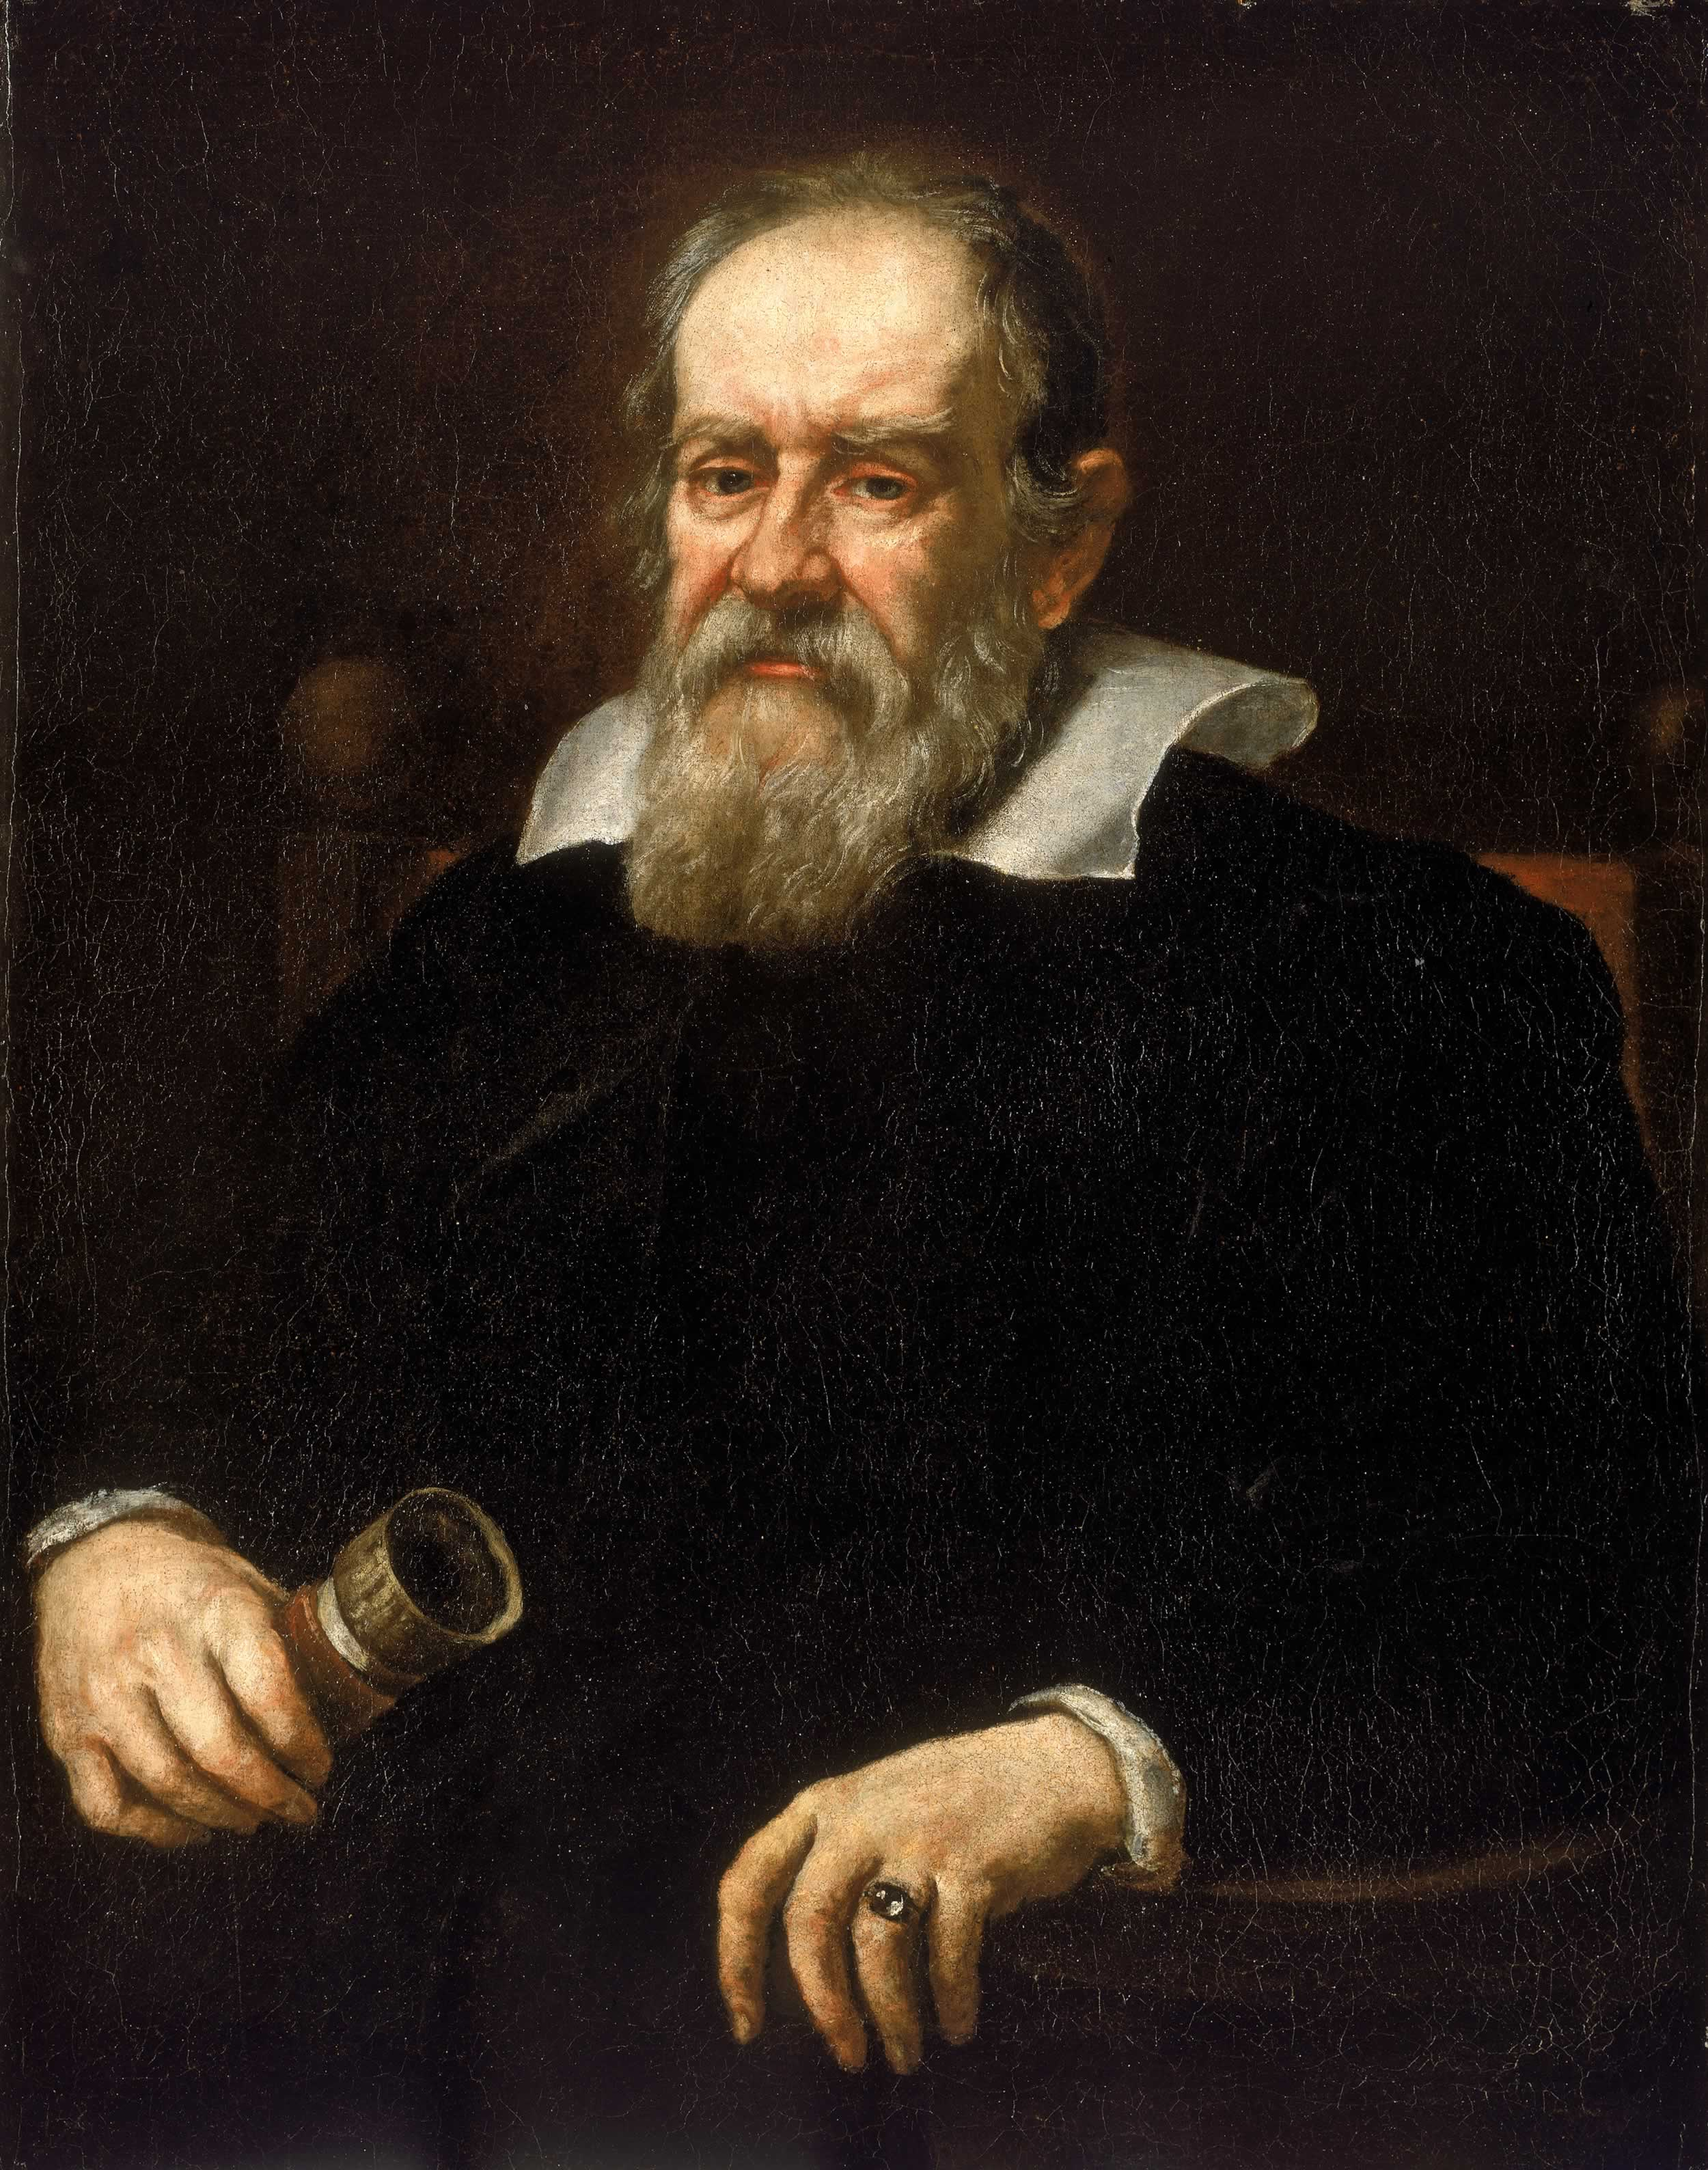
\includegraphics[width=0.95\textwidth]{images/galileo.jpg}
\captionof{figure}{Galileo Galilei (1564--1642), portrait by Justus Sustermans (1636, Uffizi Gallery).}
\end{minipage}\hfill
\begin{minipage}{0.68\textwidth}
In his 1623 treatise \emph{Il Saggiatore} (The Assayer), Galileo Galilei declared that the grand book of the universe ``cannot be understood unless one first learns to comprehend the language and read the letters in which it is composed. It is written in the language of mathematics, and its characters are triangles, circles and other geometric figures.''

By rolling bronze spheres down polished wooden inclines and measuring time with water clocks and his own pulse, Galileo dismantled the Aristotelian dogma that heavy bodies fall faster than light ones. He demonstrated that in the absence of air resistance, all bodies accelerate at identical rates, establishing kinematics as an exact experimental science.
\end{minipage}
\end{historicalbox}

\section{Physical Quantities, Dimensions, and Units}

A physical quantity $Q$ is defined as the product of a numerical magnitude $\{Q\}$ and an agreed physical measurement unit $[Q]$:
\[
Q = \{Q\}\times [Q].
\]
Mechanics is uniquely built upon three independent base dimensions:
\begin{center}
\renewcommand{\arraystretch}{1.3}
\begin{tabular}{@{}llll@{}}
\toprule
\textbf{Base Physical Dimension} & \textbf{Dimensional Symbol} & \textbf{SI Base Unit} & \textbf{Unit Symbol} \\
\midrule
Length & $\mathsf{L}$ & metre & $\mathrm{m}$ \\
Mass & $\mathsf{M}$ & kilogram & $\mathrm{kg}$ \\
Time & $\mathsf{T}$ & second & $\mathrm{s}$ \\
\bottomrule
\end{tabular}
\end{center}

All other mechanical quantities possess derived dimensions expressed as monomials:
\[
[Q] = \mathsf{L}^\alpha\,\mathsf{M}^\beta\,\mathsf{T}^\gamma, \qquad \alpha, \beta, \gamma \in \mathbb{Q}.
\]

\begin{lawbox}{Principle of Dimensional Homogeneity (Fourier, 1822)}
Any physically meaningful equation relating physical quantities $A, B, C, \dots$:
\[
f(A, B, C, \dots) = 0
\]
must be algebraically invariant under arbitrary scale transformations of the fundamental base units. Consequently, all additive terms on both sides of any valid physical equation must possess \textbf{strictly identical dimensions}.
\end{lawbox}

\section{The Buckingham $\Pi$ Theorem}

Dimensional analysis is far more than a sanity check: it is an analytical technique capable of revealing non-trivial functional dependencies when exact differential equations are unknown or intractable.

\begin{lawbox}{Buckingham $\Pi$ Theorem}
If a physical relationship involves $n$ dimensional physical variables $q_1, q_2, \dots, q_n$ that can be expressed in terms of $k$ independent fundamental dimensions, the relationship can be formulated as a function of $p = n - k$ independent \textbf{dimensionless groups} $\Pi_1, \Pi_2, \dots, \Pi_p$:
\[
\Phi(\Pi_1, \Pi_2, \dots, \Pi_{n-k}) = 0.
\]
In the special case where $n - k = 1$, the dimensionless group $\Pi_1$ must equal a pure universal constant: $\Pi_1 = C = \text{const}$.
\end{lawbox}

\section{Extensive Worked Examples}

\begin{workedexample}{G.~I.~Taylor's Blast Wave Analysis of the Trinity Nuclear Test}
In 1950, British fluid dynamicist G.~I.~Taylor published the explosive energy of the classified 1945 Trinity atomic explosion using only unclassified declassified photographs of the expanding fireball radius $R(t)$ at known time intervals $t$.
Assume the fireball radius $R$ depends solely on the total released explosive energy $E$, the ambient air density $\rho$, and the elapsed time $t$ since detonation.
(a) Determine the functional dependence $R(t, E, \rho)$ using dimensional analysis.
(b) From photographic data, at $t = 0.025\ \mathrm{s}$, the fireball radius was $R = 140\ \mathrm{m}$. Taking ambient air density $\rho \approx 1.25\ \mathrm{kg\,m^{-3}}$ and the dimensionless constant $C \approx 1.03$, calculate the blast energy $E$ in joules and kilotons of TNT ($1\ \text{kt TNT} \approx 4.184\times 10^{12}\ \mathrm{J}$).

\paragraph{Solution.}

(a) We list the variables and their dimensional formulas:
\begin{align*}
[R] &= \mathsf{L}, \\
[t] &= \mathsf{T}, \\
[\rho] &= \mathsf{M\,L^{-3}}, \\
[E] &= \mathsf{M\,L^2\,T^{-2}}.
\end{align*}
The total number of variables is $n = 4$ ($R, t, \rho, E$). The number of independent base dimensions involved is $k = 3$ ($\mathsf{L}, \mathsf{M}, \mathsf{T}$).
By the Buckingham $\Pi$ theorem, there exists $n - k = 4 - 3 = 1$ unique dimensionless group:
\[
\Pi_1 = R^\alpha\,t^\beta\,\rho^\gamma\,E^\delta.
\]
We set the overall dimension of $\Pi_1$ to unity:
\[
[\Pi_1] = \mathsf{L}^0\,\mathsf{M}^0\,\mathsf{T}^0 = (\mathsf{L})^\alpha\,(\mathsf{T})^\beta\,(\mathsf{M\,L^{-3}})^\gamma\,(\mathsf{M\,L^2\,T^{-2}})^\delta.
\]
Grouping base dimensions:
\[
\mathsf{L}^{\alpha - 3\gamma + 2\delta}\,\mathsf{M}^{\gamma + \delta}\,\mathsf{T}^{\beta - 2\delta} = \mathsf{L}^0\,\mathsf{M}^0\,\mathsf{T}^0.
\]
This yields a system of three linear equations:
\begin{align*}
\mathsf{M}:\quad & \gamma + \delta = 0 \implies \gamma = -\delta, \\
\mathsf{T}:\quad & \beta - 2\delta = 0 \implies \beta = 2\delta, \\
\mathsf{L}:\quad & \alpha - 3\gamma + 2\delta = 0 \implies \alpha - 3(-\delta) + 2\delta = 0 \implies \alpha = -5\delta.
\end{align*}
Choosing $\delta = 1$ gives $\alpha = -5$, $\beta = 2$, $\gamma = -1$. Hence:
\[
\Pi_1 = \frac{E\,t^2}{\rho\,R^5} = C = \text{constant.}
\]
Solving for the fireball radius $R(t)$:
\[
\boxed{R(t) = C^{1/5}\left(\frac{E}{\rho}\right)^{1/5} t^{2/5}.}
\]
The fireball radius expands as $t^{2/5}$!

(b) Solving for the blast energy $E$:
\[
E = \frac{1}{C}\frac{\rho\,R^5}{t^2}.
\]
With $R = 140\ \mathrm{m}$, $t = 0.025\ \mathrm{s}$, $\rho = 1.25\ \mathrm{kg\,m^{-3}}$, and $C \approx (1.03)^5 \approx 1.16$:
\begin{align*}
R^5 &= (140)^5 = 5.37824\times 10^{10}\ \mathrm{m^5}, \\
t^2 &= (0.025)^2 = 6.25\times 10^{-4}\ \mathrm{s^2}.
\end{align*}
Substituting:
\[
E = \frac{1}{1.16}\times\frac{1.25\times 5.37824\times 10^{10}}{6.25\times 10^{-4}} = \frac{1}{1.16}\times 1.0756\times 10^{14} \approx 9.27\times 10^{13}\ \mathrm{J}.
\]
In kilotons of TNT:
\[
E_{\text{TNT}} = \frac{9.27\times 10^{13}\ \mathrm{J}}{4.184\times 10^{12}\ \mathrm{J/kt}} \approx \mathbf{22.2\ \mathrm{kt\ TNT}.}
\]
Taylor's dimensional result stunned the US government because the actual classified yield was $20 \pm 2\ \mathrm{kt\ TNT}$---accurate to within $10\%$ using only elementary dimensional scaling!
\end{workedexample}

\begin{workedexample}{Phase Speed of Surface Water Waves: Deep vs Shallow Regimes}
Surface water waves propagate across a body of water of depth $h$ under gravity $g$, density $\rho$, and surface tension $\sigma$.
(a) For gravity-dominated waves ($\sigma \to 0$) where wavelength is $\lambda$, list the relevant variables for phase speed $v$.
(b) Derive the scaling of $v$ for \textbf{deep water waves} ($\lambda \ll h$, depth is irrelevant).
(c) Derive the scaling of $v$ for \textbf{shallow water waves} ($\lambda \gg h$, depth $h$ dominates over $\lambda$).

\paragraph{Solution.}

(a) In gravity-dominated waves, phase velocity $v$ can depend on wavelength $\lambda$, depth $h$, gravitational acceleration $g$, and fluid density $\rho$.
Dimensions:
\[
[v] = \mathsf{L\,T^{-1}}, \quad [\lambda] = \mathsf{L}, \quad [h] = \mathsf{L}, \quad [g] = \mathsf{L\,T^{-2}}, \quad [\rho] = \mathsf{M\,L^{-3}}.
\]
Notice that $\rho$ is the sole variable containing the mass dimension $\mathsf{M}$. To maintain dimensional homogeneity, $\rho$ must have exponent zero ($\rho^0$). Hence mass density plays no role in gravity wave velocity!

(b) \textbf{Deep water regime} ($\lambda \ll h$): The bottom is so far down that wave disturbances cannot reach it, meaning $h$ cannot enter the formula. The velocity depends only on $g$ and $\lambda$:
\[
v \propto g^\alpha\,\lambda^\beta \implies \mathsf{L\,T^{-1}} = (\mathsf{L\,T^{-2}})^\alpha\,(\mathsf{L})^\beta = \mathsf{L}^{\alpha + \beta}\,\mathsf{T}^{-2\alpha}.
\]
Equating exponents:
\[
\mathsf{T}:\ -2\alpha = -1 \implies \alpha = \frac{1}{2}, \qquad \mathsf{L}:\ \alpha + \beta = 1 \implies \beta = 1 - \frac{1}{2} = \frac{1}{2}.
\]
Therefore:
\[
\boxed{v_{\text{deep}} \propto \sqrt{g\lambda}.}
\]
Longer waves travel faster! (This dispersion causes ocean swells from distant storms to arrive well ahead of shorter choppy waves; the exact hydrodynamic factor from Airy wave theory is $\sqrt{g\lambda/2\pi}$).

(c) \textbf{Shallow water regime} ($\lambda \gg h$): For very long waves (such as ocean tsunamis), the wavelength is huge compared to ocean depth ($h \approx 4\ \mathrm{km} \ll \lambda \approx 200\ \mathrm{km}$). Thus $\lambda$ drops out and depth $h$ governs:
\[
v \propto g^\alpha\,h^\gamma \implies \alpha = \frac{1}{2},\quad \gamma = \frac{1}{2} \implies \boxed{v_{\text{shallow}} = \sqrt{gh}.}
\]
Shallow water waves are \textbf{non-dispersive}: all wavelengths travel at the identical speed $\sqrt{gh}$! For mean ocean depth $h = 4000\ \mathrm{m}$:
\[
v_{\text{tsunami}} = \sqrt{9.81\times 4000} = \sqrt{39240} \approx 198\ \mathrm{m\,s^{-1}} \approx \mathbf{713\ \mathrm{km\,h^{-1}}.}
\]
A tsunami crosses open oceans at the speed of a passenger jet aircraft.
\end{workedexample}

\begin{workedexample}{Stokes' Law vs Newton's Quadratic Drag Scaling}
A sphere of radius $R$ moves at steady speed $v$ through a fluid of dynamic viscosity $\eta$ ($[\eta] = \mathsf{M\,L^{-1}\,T^{-1}}$) and density $\rho$ ($[\rho] = \mathsf{M\,L^{-3}}$).
(a) For creeping laminar flow at very low Reynolds number ($v R \rho / \eta \ll 1$), inertia of the fluid is negligible ($\rho \to 0$). Derive the dependence of drag force $F_d$ on $R, v, \eta$.
(b) For high-speed turbulent flow ($v R \rho / \eta \gg 1$), viscosity is negligible ($\eta \to 0$). Derive the dependence of $F_d$ on $R, v, \rho$.

\paragraph{Solution.}

(a) \textbf{Laminar regime ($\rho \to 0$)}: $F_d = C_1\,\eta^\alpha\,R^\beta\,v^\gamma$.
Dimensions:
\[
[F_d] = \mathsf{M\,L\,T^{-2}} = (\mathsf{M\,L^{-1}\,T^{-1}})^\alpha\,(\mathsf{L})^\beta\,(\mathsf{L\,T^{-1}})^\gamma = \mathsf{M}^\alpha\,\mathsf{L}^{-\alpha + \beta + \gamma}\,\mathsf{T}^{-\alpha - \gamma}.
\]
Matching powers:
\begin{align*}
\mathsf{M}:\quad & \alpha = 1, \\
\mathsf{T}:\quad & -\alpha - \gamma = -2 \implies -1 - \gamma = -2 \implies \gamma = 1, \\
\mathsf{L}:\quad & -\alpha + \beta + \gamma = 1 \implies -1 + \beta + 1 = 1 \implies \beta = 1.
\end{align*}
Thus:
\[
\boxed{F_d \propto \eta\,R\,v.}
\]
The drag force is strictly \textbf{linear in velocity} and linear in size! (George Stokes' exact analytical solution gives $F_d = 6\pi\eta R v$).

(b) \textbf{Turbulent regime ($\eta \to 0$)}: $F_d = C_2\,\rho^a\,R^b\,v^c$.
Dimensions:
\[
\mathsf{M\,L\,T^{-2}} = (\mathsf{M\,L^{-3}})^a\,(\mathsf{L})^b\,(\mathsf{L\,T^{-1}})^c = \mathsf{M}^a\,\mathsf{L}^{-3a + b + c}\,\mathsf{T}^{-c}.
\]
Matching powers:
\begin{align*}
\mathsf{M}:\quad & a = 1, \\
\mathsf{T}:\quad & -c = -2 \implies c = 2, \\
\mathsf{L}:\quad & -3a + b + c = 1 \implies -3(1) + b + 2 = 1 \implies b = 2.
\end{align*}
Thus:
\[
\boxed{F_d \propto \rho\,R^2\,v^2.}
\]
Because the frontal cross-sectional area is $S = \pi R^2$, this is standard \textbf{quadratic aerodynamic drag}:
\[
F_d = \frac{1}{2}C_d\,\rho\,S\,v^2.
\]
The drag scales with the square of speed and the square of size!
\end{workedexample}

\chapter{Vector Calculus and Differential Geometry of Trajectories}
\label{ch:vectors}

\begin{chapterintro}
\textbf{Chapter Objectives:} In this chapter, we develop the mathematical machinery of vectors and vector fields that governs classical mechanics. You will master the geometry of scalar, vector, and triple products; understand Poisson's kinematic formula for rotating frames; and wield the differential vector operators ($\grad, \divg, \rot$) to determine whether physical force fields are conservative.
\end{chapterintro}

\section{Vector Algebra in Three Dimensions}

Let $\mathcal{E}^3$ be three-dimensional Euclidean space. An orthonormal Cartesian frame is defined by a fixed origin $O$ and an ordered triplet of mutually orthogonal unit vectors $(\ihat, \jhat, \khat)$ satisfying:
\[
\ihat\cdot\ihat = \jhat\cdot\jhat = \khat\cdot\khat = 1, \qquad \ihat\cdot\jhat = \jhat\cdot\khat = \khat\cdot\ihat = 0, \qquad \ihat\times\jhat = \khat.
\]

\begin{figure}[htbp]
\centering
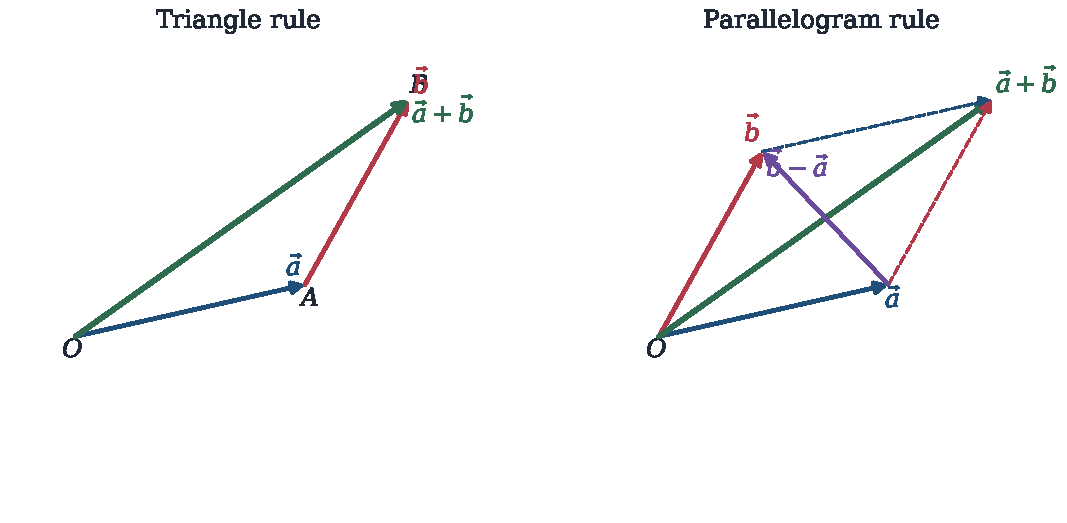
\includegraphics[width=0.74\textwidth]{figures/01_vector_addition.pdf}
\caption{Vector addition and scalar multiplication in Euclidean space. The triangle and parallelogram constructions illustrate $\vec{A} + \vec{B}$.}
\label{fig:vector_addition}
\end{figure}

Any vector $\vec{A}$ can be uniquely resolved into its Cartesian scalar components:
\[
\vec{A} = A_x\,\ihat + A_y\,\jhat + A_z\,\khat.
\]
The Euclidean norm (magnitude) is:
\[
\norm{\vec{A}} = A = \sqrt{\vec{A}\cdot\vec{A}} = \sqrt{A_x^2 + A_y^2 + A_z^2}.
\]

\section{Products of Vectors}

\begin{figure}[htbp]
\centering
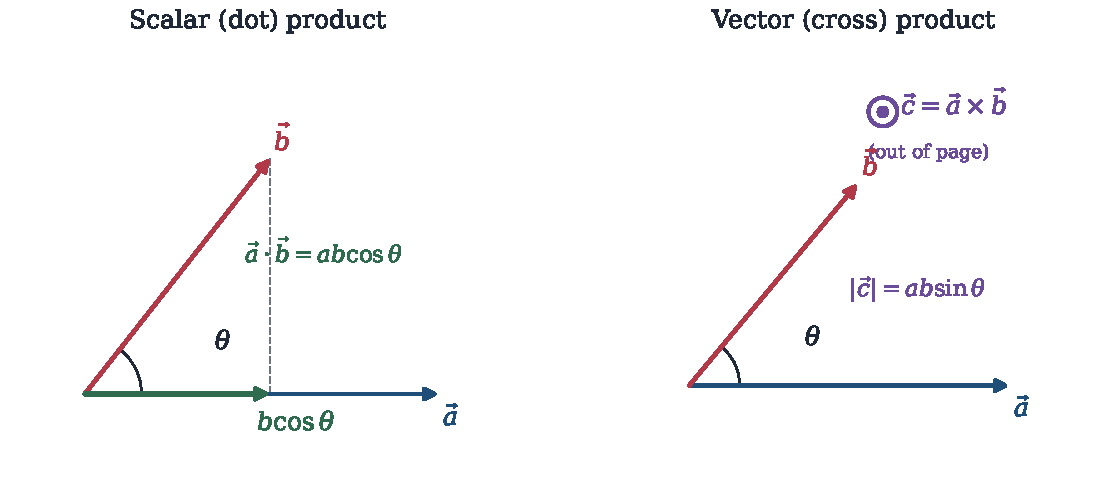
\includegraphics[width=0.78\textwidth]{figures/03_dot_cross.pdf}
\caption{The scalar product $\vec{A}\cdot\vec{B} = AB\cos\theta$ measures collinear projection; the vector product $\vec{A}\times\vec{B}$ yields an orthogonal vector of magnitude $AB\sin\theta$ representing the oriented area of the spanned parallelogram.}
\label{fig:dot_cross}
\end{figure}

\begin{definitionbox}{The Scalar Product (Dot Product)}
The scalar product of two vectors $\vec{A}$ and $\vec{B}$ separated by angle $\theta \in [0, \pi]$ is:
\[
\boxed{\vec{A}\cdot\vec{B} = \norm{\vec{A}}\,\norm{\vec{B}}\cos\theta = A_x B_x + A_y B_y + A_z B_z.}
\]
Two non-zero vectors are orthogonal if and only if $\vec{A}\cdot\vec{B} = 0$.
\end{definitionbox}

\begin{definitionbox}{The Vector Product (Cross Product)}
The vector product $\vec{A}\times\vec{B}$ is a vector orthogonal to both $\vec{A}$ and $\vec{B}$, oriented by the right-hand rule, with magnitude equal to the area of the parallelogram spanned by $\vec{A}$ and $\vec{B}$:
\[
\norm{\vec{A}\times\vec{B}} = \norm{\vec{A}}\,\norm{\vec{B}}\sin\theta.
\]
In Cartesian components, it is expressed as a formal determinant:
\[
\boxed{\vec{A}\times\vec{B} = \begin{vmatrix} \ihat & \jhat & \khat \\ A_x & A_y & A_z \\ B_x & B_y & B_z \end{vmatrix} = (A_y B_z - A_z B_y)\ihat + (A_z B_x - A_x B_z)\jhat + (A_x B_y - A_y B_x)\khat.}
\]
The cross product is anticommutative: $\vec{B}\times\vec{A} = -\vec{A}\times\vec{B}$.
\end{definitionbox}

\begin{lawbox}{The Triple Products and the BAC--CAB Identity}
\begin{itemize}[leftmargin=1.4em,itemsep=3pt]
  \item \textbf{Scalar Triple Product}: $\vec{A}\cdot(\vec{B}\times\vec{c}) = \det[\vec{A}, \vec{B}, \vec{C}]$ represents the oriented volume of the parallelepiped spanned by the three vectors. It is invariant under cyclic permutations:
        \[
        \vec{A}\cdot(\vec{B}\times\vec{C}) = \vec{B}\cdot(\vec{C}\times\vec{A}) = \vec{C}\cdot(\vec{A}\times\vec{B}).
        \]
  \item \textbf{Vector Triple Product (BAC--CAB Rule)}:
        \[
        \boxed{\vec{A}\times(\vec{B}\times\vec{C}) = (\vec{A}\cdot\vec{C})\vec{B} - (\vec{A}\cdot\vec{B})\vec{C}.}
        \]
\end{itemize}
\end{lawbox}

\section{Vector Functions of Time and Poisson's Formula}

When a vector $\vec{A}(t)$ varies with time, its derivative is defined by the standard limit:
\[
\frac{\dd\vec{A}}{\dd t} = \lim_{\Delta t \to 0} \frac{\vec{A}(t + \Delta t) - \vec{A}(t)}{\Delta t} = \dot{A}_x\,\ihat + \dot{A}_y\,\jhat + \dot{A}_z\,\khat.
\]
Differentiating products yields Leibniz rules:
\begin{align*}
\frac{\dd}{\dd t}(\phi\vec{A}) &= \dot{\phi}\vec{A} + \phi\dot{\vec{A}}, \\
\frac{\dd}{\dd t}(\vec{A}\cdot\vec{B}) &= \dot{\vec{A}}\cdot\vec{B} + \vec{A}\cdot\dot{\vec{B}}, \\
\frac{\dd}{\dd t}(\vec{A}\times\vec{B}) &= \dot{\vec{A}}\times\vec{B} + \vec{A}\times\dot{\vec{B}} \quad \text{(order preserved!).}
\end{align*}

\begin{lawbox}{Poisson's Kinematic Formula for Rotating Vectors}
Let $\vec{u}(t)$ be a unit vector of constant length ($\norm{\vec{u}(t)} \equiv 1$).
Then $\vec{u}\cdot\vec{u} = 1$. Differentiating with respect to time:
\[
\frac{\dd}{\dd t}(\vec{u}\cdot\vec{u}) = 2\vec{u}\cdot\frac{\dd\vec{u}}{\dd t} = 0 \implies \frac{\dd\vec{u}}{\dd t} \perp \vec{u}.
\]
Every derivative of a constant-length vector is strictly orthogonal to the vector itself!
Consequently, for any rotating rigid frame with angular velocity vector $\vec{\Omega}$, the rate of change of any vector $\vec{A}$ attached to that frame satisfies:
\[
\boxed{\frac{\dd\vec{A}}{\dd t} = \vec{\Omega}\times\vec{A}.}
\]
\end{lawbox}

\section{Differential Operators in Physics}

In field theories of mechanics, forces are functions of position $\vec{r}$. We define the formal vector differential operator \textbf{del} (nabla):
\[
\vec{\nabla} \equiv \frac{\partial}{\partial x}\ihat + \frac{\partial}{\partial y}\jhat + \frac{\partial}{\partial z}\khat.
\]

\begin{definitionbox}{Gradient, Divergence, and Curl}
\begin{itemize}[leftmargin=1.4em,itemsep=3pt]
  \item \textbf{Gradient} of a scalar field $f(x, y, z)$:
        \[
        \grad f = \vec{\nabla} f = \frac{\partial f}{\partial x}\ihat + \frac{\partial f}{\partial y}\jhat + \frac{\partial f}{\partial z}\khat.
        \]
        $\vec{\nabla} f$ points in the direction of steepest spatial increase of $f$, and its magnitude is the directional derivative in that direction.
  \item \textbf{Divergence} of a vector field $\vec{V}(x, y, z)$:
        \[
        \divg \vec{V} = \vec{\nabla}\cdot\vec{V} = \frac{\partial V_x}{\partial x} + \frac{\partial V_y}{\partial y} + \frac{\partial V_z}{\partial z}.
        \]
        $\vec{\nabla}\cdot\vec{V}$ measures the net flux of $\vec{V}$ emanating per unit volume from a point (sources and sinks).
  \item \textbf{Curl (Rotationnel)} of a vector field $\vec{V}(x, y, z)$:
        \[
        \rot \vec{V} = \vec{\nabla}\times\vec{V} = \begin{vmatrix} \ihat & \jhat & \khat \\ \partial/\partial x & \partial/\partial y & \partial/\partial z \\ V_x & V_y & V_z \end{vmatrix}.
        \]
        $\vec{\nabla}\times\vec{V}$ measures the microscopic circulation or vortex density of the vector field.
\end{itemize}
\end{definitionbox}

\begin{lawbox}{The Irrotational Gradient Identity}
For any twice continuously differentiable scalar function $f(x, y, z)$:
\[
\boxed{\vec{\nabla}\times(\vec{\nabla} f) = \vzero.}
\]
\textbf{Physical Meaning:} Every gradient field is automatically curl-free (irrotational).
Conversely, by Poincaré's Lemma, if a force field $\vec{F}$ is curl-free in a simply-connected domain ($\vec{\nabla}\times\vec{F} = \vzero$), then there exists a potential energy function $E_p(\vec{r})$ such that $\vec{F} = -\vec{\nabla} E_p$.
\end{lawbox}

\section{Extensive Worked Examples}

\begin{workedexample}{The BAC--CAB Expansion and Jacobi Identity}
(a) Prove the BAC--CAB identity $\vec{A}\times(\vec{B}\times\vec{C}) = (\vec{A}\cdot\vec{C})\vec{B} - (\vec{A}\cdot\vec{B})\vec{C}$.
(b) Deduce the \textbf{Jacobi Identity} for the cross product:
\[
\vec{A}\times(\vec{B}\times\vec{C}) + \vec{B}\times(\vec{C}\times\vec{A}) + \vec{C}\times(\vec{A}\times\vec{B}) = \vzero.
\]

\paragraph{Solution.}

(a) Without loss of generality, choose Cartesian coordinates such that $\vec{B}$ lies along the $x$-axis: $\vec{B} = B_x\ihat$, and $\vec{C}$ lies in the $xy$-plane: $\vec{C} = C_x\ihat + C_y\jhat$.
Let $\vec{A} = A_x\ihat + A_y\jhat + A_z\khat$.
The inner cross product is:
\[
\vec{B}\times\vec{C} = (B_x\ihat)\times(C_x\ihat + C_y\jhat) = B_x C_y(\ihat\times\jhat) = B_x C_y\,\khat.
\]
Now compute $\vec{A}\times(\vec{B}\times\vec{C})$:
\begin{align*}
\vec{A}\times(B_x C_y\,\khat) &= (A_x\ihat + A_y\jhat + A_z\khat)\times(B_x C_y\,\khat) \\
&= A_x B_x C_y(\ihat\times\khat) + A_y B_x C_y(\jhat\times\khat) \\
&= -A_x B_x C_y\,\jhat + A_y B_x C_y\,\ihat.
\end{align*}
Now compute the right-hand side $(\vec{A}\cdot\vec{C})\vec{B} - (\vec{A}\cdot\vec{B})\vec{C}$:
\begin{align*}
\vec{A}\cdot\vec{C} &= A_x C_x + A_y C_y, \\
\vec{A}\cdot\vec{B} &= A_x B_x.
\end{align*}
Thus:
\begin{align*}
(\vec{A}\cdot\vec{C})\vec{B} - (\vec{A}\cdot\vec{B})\vec{C} &= (A_x C_x + A_y C_y)(B_x\ihat) - (A_x B_x)(C_x\ihat + C_y\jhat) \\
&= A_x B_x C_x\ihat + A_y B_x C_y\ihat - A_x B_x C_x\ihat - A_x B_x C_y\jhat \\
&= A_y B_x C_y\ihat - A_x B_x C_y\jhat.
\end{align*}
Both expressions are identical! Since the statement is coordinate-independent, the BAC--CAB rule is proven in full generality.

(b) Applying the BAC--CAB rule cyclically to all three permutations:
\begin{align*}
\vec{A}\times(\vec{B}\times\vec{C}) &= (\vec{A}\cdot\vec{C})\vec{B} - (\vec{A}\cdot\vec{B})\vec{C}, \\
\vec{B}\times(\vec{C}\times\vec{A}) &= (\vec{B}\cdot\vec{A})\vec{C} - (\vec{B}\cdot\vec{C})\vec{A}, \\
\vec{C}\times(\vec{A}\times\vec{B}) &= (\vec{C}\cdot\vec{B})\vec{A} - (\vec{C}\cdot\vec{A})\vec{B}.
\end{align*}
Adding all three equations:
Since the dot product is symmetric ($\vec{A}\cdot\vec{C} = \vec{C}\cdot\vec{A}$, $\vec{A}\cdot\vec{B} = \vec{B}\cdot\vec{A}$, $\vec{B}\cdot\vec{C} = \vec{C}\cdot\vec{B}$), every positive term cancels with an identical negative term:
\[
\boxed{\vec{A}\times(\vec{B}\times\vec{C}) + \vec{B}\times(\vec{C}\times\vec{A}) + \vec{C}\times(\vec{A}\times\vec{B}) = \vzero.}
\]
This Jacobi identity confirms that the 3D cross product forms a formal Lie algebra $\mathfrak{so}(3)$ isomorphic to the group of physical rotations!
\end{workedexample}

\begin{workedexample}{Gradient and Curl of Central Force Fields}
Let $\vec{r} = x\ihat + y\jhat + z\khat$ be the position vector, with magnitude $r = \norm{\vec{r}} = \sqrt{x^2 + y^2 + z^2}$, and unit vector $\ur = \vec{r}/r$.
(a) Show that $\vec{\nabla} r = \ur$.
(b) Show that $\vec{\nabla} f(r) = f'(r)\ur$.
(c) Show that any central force field $\vec{F}(\vec{r}) = f(r)\ur$ is irrotational: $\vec{\nabla}\times\vec{F} = \vzero$.
(d) Find the potential energy $E_p(r)$ for Newton's gravitational force $\vec{F}(\vec{r}) = -\frac{GMm}{r^2}\ur$.

\paragraph{Solution.}

(a) Compute the partial derivatives of $r = \sqrt{x^2 + y^2 + z^2}$:
\[
\frac{\partial r}{\partial x} = \frac{2x}{2\sqrt{x^2 + y^2 + z^2}} = \frac{x}{r}, \quad \frac{\partial r}{\partial y} = \frac{y}{r}, \quad \frac{\partial r}{\partial z} = \frac{z}{r}.
\]
Therefore:
\[
\vec{\nabla} r = \frac{\partial r}{\partial x}\ihat + \frac{\partial r}{\partial y}\jhat + \frac{\partial r}{\partial z}\khat = \frac{x}{r}\ihat + \frac{y}{r}\jhat + \frac{z}{r}\khat = \frac{\vec{r}}{r} = \boxed{\ur.}
\]

(b) Applying the chain rule to an arbitrary scalar function $f(r)$:
\[
\frac{\partial f}{\partial x} = \frac{\dd f}{\dd r}\frac{\partial r}{\partial x} = f'(r)\frac{x}{r}.
\]
Assembling the gradient:
\[
\vec{\nabla} f(r) = f'(r)\left(\frac{x}{r}\ihat + \frac{y}{r}\jhat + \frac{z}{r}\khat\right) = \boxed{f'(r)\,\ur.}
\]

(c) We compute the curl of $\vec{F} = f(r)\ur = \frac{f(r)}{r}\vec{r}$.
Using the vector identity $\vec{\nabla}\times(\phi\vec{A}) = \phi(\vec{\nabla}\times\vec{A}) + (\vec{\nabla}\phi)\times\vec{A}$ with $\phi = \frac{f(r)}{r}$ and $\vec{A} = \vec{r}$:
First, compute $\vec{\nabla}\times\vec{r}$:
\[
\vec{\nabla}\times\vec{r} = \begin{vmatrix} \ihat & \jhat & \khat \\ \partial/\partial x & \partial/\partial y & \partial/\partial z \\ x & y & z \end{vmatrix} = (0 - 0)\ihat + (0 - 0)\jhat + (0 - 0)\khat = \vzero.
\]
Second, compute the gradient of the scalar factor $\phi(r)$:
\[
\vec{\nabla}\phi(r) = \phi'(r)\ur.
\]
Now substitute into the identity:
\[
\vec{\nabla}\times\left( \frac{f(r)}{r}\vec{r} \right) = \frac{f(r)}{r}(\vzero) + \left( \phi'(r)\ur \right)\times\vec{r} = \phi'(r)(\ur\times\vec{r}).
\]
Since $\vec{r} = r\ur$, the cross product is:
\[
\ur\times\vec{r} = r(\ur\times\ur) = \vzero.
\]
Therefore:
\[
\boxed{\vec{\nabla}\times\vec{F} = \vzero.}
\]
Every central force field is strictly \textbf{curl-free (conservative)}!

(d) For Newton's gravitational force:
\[
\vec{F}(r) = -\frac{GMm}{r^2}\ur.
\]
Since $\vec{F} = -\vec{\nabla} E_p = -E_p'(r)\ur$:
\[
-E_p'(r) = -\frac{GMm}{r^2} \implies E_p'(r) = \frac{GMm}{r^2}.
\]
Integrating with standard reference at infinity ($E_p(\infty) = 0$):
\[
E_p(r) = -\int_\infty^r \frac{GMm}{r'^2}\dd r' = -\left[ -\frac{GMm}{r'} \right]_\infty^r = \boxed{-\frac{GMm}{r}.}
\]
\end{workedexample}

\chapter{One-Dimensional Kinematics and Motion with Drag}
\label{ch:kinematics_1d}

\begin{chapterintro}
\textbf{Chapter Objectives:} In this chapter, we develop the differential and integral calculus of one-dimensional motion. You will master the inversion of acceleration functions $a(t)$, $a(v)$, and $a(x)$; read kinematic graphs; solve motion under linear and quadratic fluid resistance; derive terminal velocities; and prove why vertical projectiles spend more time descending than ascending.
\end{chapterintro}

\section{Fundamental Definitions of 1D Motion}

Consider a particle constrained to move along a straight line chosen as the $x$-axis.
\begin{itemize}[leftmargin=1.4em,itemsep=3pt]
  \item \textbf{Position}: $x(t) \in \mathbb{R}$ relative to origin $O$.
  \item \textbf{Displacement}: $\Delta x = x(t_2) - x(t_1)$.
  \item \textbf{Instantaneous Velocity}:
        \[
        \boxed{v(t) = \lim_{\Delta t\to 0}\frac{\Delta x}{\Delta t} = \frac{\dd x}{\dd t} = \dot{x}(t).}
        \]
  \item \textbf{Instantaneous Acceleration}:
        \[
        \boxed{a(t) = \lim_{\Delta t\to 0}\frac{\Delta v}{\Delta t} = \frac{\dd v}{\dd t} = \frac{\dd^2 x}{\dd t^2} = \ddot{x}(t).}
        \]
\end{itemize}

\begin{figure}[htbp]
\centering
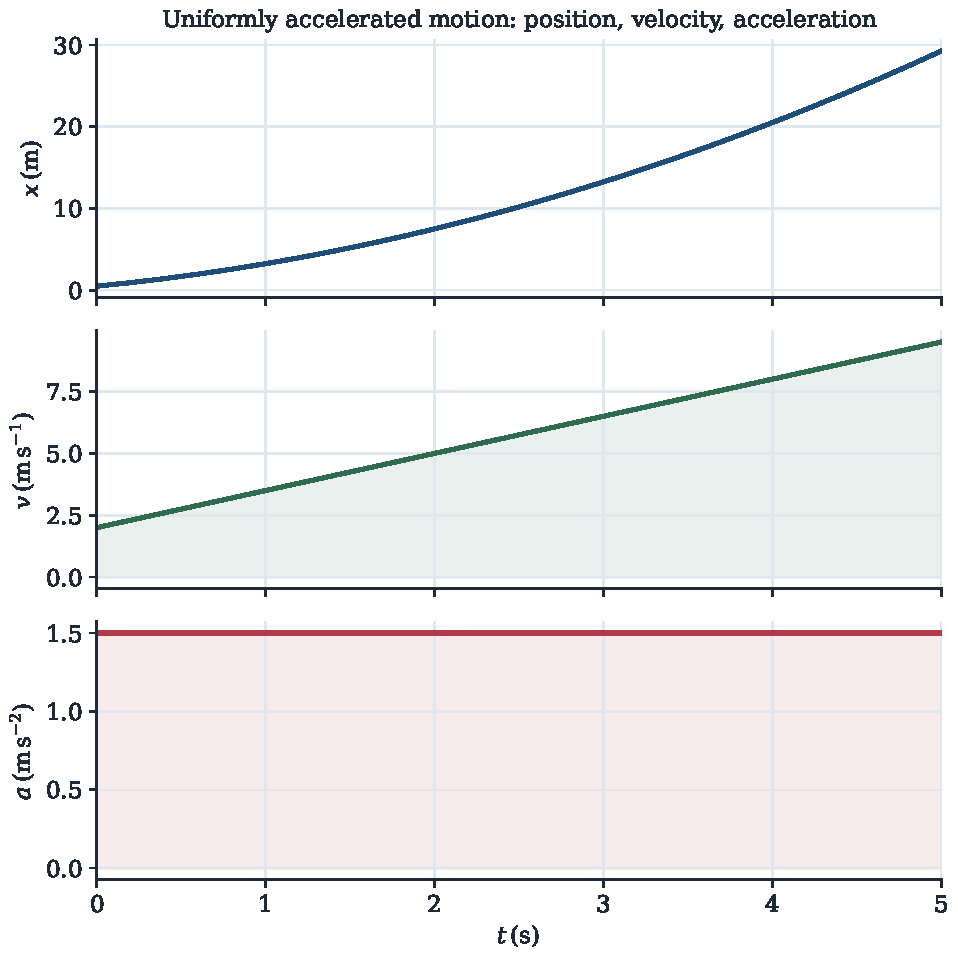
\includegraphics[width=0.88\textwidth]{figures/05_motion_graphs.pdf}
\caption{Kinematic graphs in 1D. The velocity is the slope of $x(t)$; the displacement is the area under $v(t)$; the acceleration is the slope of $v(t)$.}
\label{fig:motion_graphs}
\end{figure}

\section{The Three Standard Integration Protocols}

In general physical problems, acceleration is not constant but depends on time $t$, velocity $v$, or position $x$:

\begin{center}
\renewcommand{\arraystretch}{1.4}
\begin{tabular}{@{}lll@{}}
\toprule
\textbf{Given Acceleration} & \textbf{Separation of Variables} & \textbf{Integral Formula} \\
\midrule
$a = a(t)$ & $\dd v = a(t)\,\dd t$ & $v(t) = v_0 + \int_0^t a(t')\,\dd t'$ \\
$a = a(v)$ & $\dd t = \frac{\dd v}{a(v)}, \quad \dd x = \frac{v\,\dd v}{a(v)}$ & $t(v) = \int_{v_0}^v \frac{\dd v'}{a(v')}, \quad x(v) = x_0 + \int_{v_0}^v \frac{v'\,\dd v'}{a(v')}$ \\
$a = a(x)$ & $v\,\dd v = a(x)\,\dd x$ & $v^2(x) = v_0^2 + 2\int_{x_0}^x a(x')\,\dd x'$ \\
\bottomrule
\end{tabular}
\end{center}

\begin{lawbox}{The Chain Rule Identity for Acceleration}
By the chain rule:
\[
\boxed{a = \frac{\dd v}{\dd t} = \frac{\dd v}{\dd x}\frac{\dd x}{\dd t} = v\frac{\dd v}{\dd x} = \frac{\dd}{\dd x}\left(\frac{1}{2}v^2\right).}
\]
This timeless relation connects acceleration directly to spatial displacement without reference to time.
\end{lawbox}

\section{Motion with Fluid Resistance}

\begin{figure}[htbp]
\centering
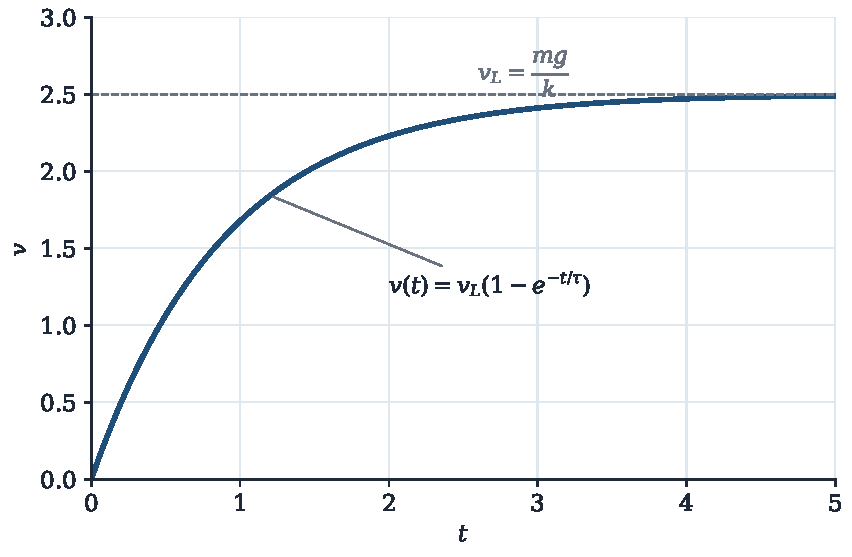
\includegraphics[width=0.74\textwidth]{figures/19_terminal_velocity.pdf}
\caption{Vertical fall under gravity with drag. The velocity asymptotically approaches terminal velocity $v_t$ where drag balances weight.}
\label{fig:terminal_velocity}
\end{figure}

When a body moves through a fluid, it experiences a resistive drag force opposing its velocity:
\begin{itemize}[leftmargin=1.4em,itemsep=3pt]
  \item \textbf{Linear (Stokes) Drag} ($F_d = -b v$): Operates at low velocities and tiny scales (pollen grains, mist droplets, oil droplets in Millikan's experiment).
  \item \textbf{Quadratic (Newton) Drag} ($F_d = -c v^2$): Operates at macroscopic scales and everyday speeds (baseballs, skydivers, automobiles, airplanes).
\end{itemize}

\section{Extensive Worked Examples}

\begin{workedexample}{Vertical Fall with Linear Drag (Exact Solution)}
A particle of mass $m$ is released from rest at $t = 0$ in a gravitational field $g$ subject to a linear viscous drag force $F_d = -b v$.
(a) Write the differential equation of motion and identify the characteristic velocity $v_t$ and time scale $\tau$.
(b) Solve for the instantaneous velocity $v(t)$.
(c) Integrate $v(t)$ to obtain the position $z(t)$.
(d) Examine the short-time ($t \ll \tau$) and long-time ($t \gg \tau$) limits.

\paragraph{Solution.}

(a) Orient the vertical $z$-axis downward, so gravity is $+mg$ and drag is $-bv$.
Newton's second law:
\[
m\frac{\dd v}{\dd t} = mg - bv \implies \frac{\dd v}{\dd t} = g - \frac{b}{m}v = -\frac{b}{m}\left(v - \frac{mg}{b}\right).
\]
Define the \textbf{characteristic time constant} $\tau$ and \textbf{terminal velocity} $v_t$:
\[
\boxed{\tau = \frac{m}{b}}, \qquad \boxed{v_t = \frac{mg}{b} = g\tau.}
\]
Then the equation becomes:
\[
\frac{\dd v}{\dd t} = -\frac{1}{\tau}(v - v_t).
\]

(b) Separating variables:
\[
\frac{\dd v}{v - v_t} = -\frac{\dd t}{\tau}.
\]
Integrating with initial condition $v(0) = 0$:
\[
\int_0^v \frac{\dd v'}{v' - v_t} = -\frac{1}{\tau}\int_0^t \dd t' \implies \ln\left(\frac{v - v_t}{-v_t}\right) = -\frac{t}{\tau} \implies 1 - \frac{v}{v_t} = e^{-t/\tau}.
\]
Solving for $v(t)$:
\[
\boxed{v(t) = v_t\left(1 - e^{-t/\tau}\right).}
\]

(c) Integrating $v(t) = \frac{\dd z}{\dd t}$ with $z(0) = 0$:
\[
z(t) = \int_0^t v_t\left(1 - e^{-t'/\tau}\right)\dd t' = v_t\left[ t' + \tau e^{-t'/\tau} \right]_0^t = \boxed{v_t t - v_t\tau\left(1 - e^{-t/\tau}\right).}
\]

(d) \textbf{Asymptotic limits:}
\begin{itemize}[leftmargin=1.4em,itemsep=2pt]
  \item \textbf{Short-time limit ($t \ll \tau$)}: Expand the exponential $e^{-t/\tau} \approx 1 - \frac{t}{\tau} + \frac{t^2}{2\tau^2}$:
  \[
  v(t) = v_t\left[ 1 - \left(1 - \frac{t}{\tau} + \frac{t^2}{2\tau^2}\right) \right] \approx v_t\frac{t}{\tau} = (g\tau)\frac{t}{\tau} = gt.
  \]
  \[
  z(t) \approx v_t t - v_t\tau\left[ \frac{t}{\tau} - \frac{t^2}{2\tau^2} \right] = v_t t - v_t t + \frac{1}{2}\frac{v_t}{\tau}t^2 = \frac{1}{2}gt^2.
  \]
  At initial times, drag is negligible, recovering pure vacuum free fall!
  \item \textbf{Long-time limit ($t \gg \tau$)}: The exponential term decays to zero ($e^{-t/\tau} \to 0$):
  \[
  v(t) \to v_t = \text{const}, \qquad z(t) \to v_t t - v_t\tau.
  \]
  The particle moves at constant terminal velocity $v_t$, with a spatial delay $v_t\tau$ representing the initial acceleration phase.
\end{itemize}
\end{workedexample}

\begin{workedexample}{Vertical Fall with Quadratic Drag (Hyperbolic Solution)}
A skydiver of mass $m$ falls from rest under quadratic aerodynamic drag $F_d = -c v^2$.
(a) Determine the terminal velocity $v_t$.
(b) Integrate the equation of motion using separation of variables to show:
\[
v(t) = v_t\tanh\left(\frac{gt}{v_t}\right).
\]
(c) Find the distance fallen $z(t)$ and the timeless relation $v(z)$.

\paragraph{Solution.}

(a) Downward equation of motion:
\[
m\frac{\dd v}{\dd t} = mg - cv^2.
\]
At terminal velocity, acceleration vanishes:
\[
mg - cv_t^2 = 0 \implies \boxed{v_t = \sqrt{\frac{mg}{c}}.}
\]
Rewriting the equation of motion using $c/m = g/v_t^2$:
\[
\frac{\dd v}{\dd t} = g\left(1 - \frac{v^2}{v_t^2}\right).
\]

(b) Separating variables:
\[
\frac{\dd v}{1 - (v/v_t)^2} = g\,\dd t.
\]
Using the standard integral $\int \frac{\dd u}{1 - u^2} = \operatorname{artanh}(u)$:
\[
v_t\int_0^{v/v_t} \frac{\dd u}{1 - u^2} = gt \implies v_t\operatorname{artanh}\left(\frac{v}{v_t}\right) = gt.
\]
Taking the hyperbolic tangent of both sides:
\[
\boxed{v(t) = v_t\tanh\left(\frac{gt}{v_t}\right).}
\]
Since $\tanh(x) \to 1$ as $x \to \infty$, the speed smoothly approaches $v_t$. At $t = 2v_t/g$, $\tanh(2) \approx 0.964$: the skydiver reaches over $96\%$ of terminal velocity in roughly two time constants.

(c) Distance fallen:
\[
z(t) = \int_0^t v(t')\dd t' = v_t\int_0^t \tanh\left(\frac{gt'}{v_t}\right)\dd t'.
\]
Using $\int \tanh(ax)\dd x = \frac{1}{a}\ln\cosh(ax)$:
\[
\boxed{z(t) = \frac{v_t^2}{g}\ln\cosh\left(\frac{gt}{v_t}\right).}
\]
For the spatial relation $v(z)$, use $v\frac{\dd v}{\dd z} = g\left(1 - \frac{v^2}{v_t^2}\right)$:
\[
\frac{v\,\dd v}{1 - v^2/v_t^2} = g\,\dd z.
\]
Let $w = 1 - v^2/v_t^2 \implies \dd w = -\frac{2v}{v_t^2}\dd v$:
\[
-\frac{v_t^2}{2}\int_1^{1 - v^2/v_t^2} \frac{\dd w}{w} = gz \implies -\frac{v_t^2}{2}\ln\left(1 - \frac{v^2}{v_t^2}\right) = gz.
\]
Exponentiating:
\[
1 - \frac{v^2}{v_t^2} = e^{-2gz/v_t^2} \implies \boxed{v(z) = v_t\sqrt{1 - e^{-2gz/v_t^2}}.}
\]
\end{workedexample}

\begin{workedexample}{Asymmetry of Ascent and Descent under Quadratic Drag}
A projectile is fired vertically upward with initial speed $v_0$ in air with quadratic drag $c v^2$.
(a) Find the maximum height $H$ reached by the projectile.
(b) Find the time of ascent $t_{\text{up}}$.
(c) The projectile falls back down from height $H$ to the ground. Find its landing speed $v_{\text{land}}$ and time of descent $t_{\text{down}}$.
(d) Prove that $t_{\text{down}} > t_{\text{up}}$: the projectile always spends more time coming down than going up!

\paragraph{Solution.}

(a) During ascent (upward $y$-axis): both gravity and drag point downward:
\[
m\frac{\dd v}{\dd t} = -mg - cv^2 = -mg\left(1 + \frac{v^2}{v_t^2}\right).
\]
Using $v\frac{\dd v}{\dd y} = -g\left(1 + \frac{v^2}{v_t^2}\right)$ from $(y=0, v=v_0)$ to $(y=H, v=0)$:
\[
\int_{v_0}^0 \frac{v\,\dd v}{1 + v^2/v_t^2} = -g\int_0^H \dd y \implies \left[ \frac{v_t^2}{2}\ln\left(1 + \frac{v^2}{v_t^2}\right) \right]_{v_0}^0 = -gH.
\]
\[
-\frac{v_t^2}{2}\ln\left(1 + \frac{v_0^2}{v_t^2}\right) = -gH \implies \boxed{H = \frac{v_t^2}{2g}\ln\left(1 + \frac{v_0^2}{v_t^2}\right).}
\]

(b) For time of ascent:
\[
\frac{\dd v}{\dd t} = -g\left(1 + \frac{v^2}{v_t^2}\right) \implies \int_{v_0}^0 \frac{\dd v}{1 + (v/v_t)^2} = -g\int_0^{t_{\text{up}}}\dd t.
\]
Using $\int \frac{\dd u}{1 + u^2} = \arctan(u)$:
\[
v_t\left[ 0 - \arctan\left(\frac{v_0}{v_t}\right) \right] = -gt_{\text{up}} \implies \boxed{t_{\text{up}} = \frac{v_t}{g}\arctan\left(\frac{v_0}{v_t}\right).}
\]

(c) During descent from rest at height $H$:
From Example 3.2, the landing speed satisfies $v_{\text{land}} = v_t\sqrt{1 - e^{-2gH/v_t^2}}$.
Substitute $e^{-2gH/v_t^2} = \frac{1}{1 + v_0^2/v_t^2}$:
\[
v_{\text{land}} = v_t\sqrt{1 - \frac{1}{1 + v_0^2/v_t^2}} = v_t\sqrt{\frac{v_0^2/v_t^2}{1 + v_0^2/v_t^2}} = \boxed{\frac{v_0}{\sqrt{1 + v_0^2/v_t^2}} < v_0.}
\]
The landing speed is strictly smaller than the launch speed due to dissipated mechanical energy!
For descent time, from $v(t) = v_t\tanh(gt/v_t)$:
\[
\tanh\left(\frac{gt_{\text{down}}}{v_t}\right) = \frac{v_{\text{land}}}{v_t} = \frac{v_0/v_t}{\sqrt{1 + v_0^2/v_t^2}}.
\]
Using the identity $\operatorname{artanh}\left(\frac{x}{\sqrt{1+x^2}}\right) = \operatorname{arsinh}(x)$:
\[
\boxed{t_{\text{down}} = \frac{v_t}{g}\operatorname{arsinh}\left(\frac{v_0}{v_t}\right).}
\]

(d) To compare $t_{\text{up}}$ and $t_{\text{down}}$, define $\xi = v_0/v_t > 0$:
\[
t_{\text{up}} = \frac{v_t}{g}\arctan(\xi), \qquad t_{\text{down}} = \frac{v_t}{g}\operatorname{arsinh}(\xi).
\]
For any $\xi > 0$, we have:
\[
\operatorname{arsinh}(\xi) = \ln\left(\xi + \sqrt{1+\xi^2}\right) > \arctan(\xi).
\]
(Indeed, $\frac{\dd}{\dd\xi}\operatorname{arsinh}\xi = \frac{1}{\sqrt{1+\xi^2}} > \frac{1}{1+\xi^2} = \frac{\dd}{\dd\xi}\arctan\xi$ for all $\xi > 0$, and both are zero at $\xi=0$).
Therefore:
\[
\boxed{t_{\text{down}} > t_{\text{up}}.}
\]
The projectile \textbf{always takes longer to fall down than to rise}!
On the way up, gravity and drag cooperate (both pull downward, producing large decelerations $> g$). On the way down, drag opposes gravity (deceleration is $< g$). Consequently, average speed during descent is lower, requiring a longer transit time.
\end{workedexample}

\chapter{Two- and Three-Dimensional Kinematics, Projectiles, and Circles}
\label{ch:kinematics_2d3d}

\begin{chapterintro}
\textbf{Chapter Objectives:} In this chapter, we extend kinematics to multi-dimensional trajectories. You will master the principle of independent orthogonal motions; derive the Cartesian equations, range, and vertex of projectile paths; compute the Parabola of Safety separating reachable and unreachable domains; analyze circular motion and centripetal acceleration; and construct velocity hodographs.
\end{chapterintro}

\section{Planar Motion in Cartesian Coordinates}

When a particle moves in a plane, its instantaneous state is described by position vector $\vec{r}(t) = x(t)\ihat + y(t)\jhat$.
The velocity and acceleration are:
\[
\vec{v}(t) = \dot{x}\ihat + \dot{y}\jhat, \qquad \vec{a}(t) = \ddot{x}\ihat + \ddot{y}\jhat.
\]
The magnitude of velocity (speed) is $v = \norm{\vec{v}} = \sqrt{\dot{x}^2 + \dot{y}^2}$, and the direction of motion makes an angle $\theta(t)$ with the horizontal:
\[
\tan\theta(t) = \frac{\dot{y}(t)}{\dot{x}(t)}.
\]

\begin{lawbox}{Galilean Independence of Orthogonal Motions}
Motion along the horizontal $x$-axis and vertical $y$-axis are dynamically and kinematically \textbf{independent}. The time parameter $t$ serves as the sole coupling link between orthogonal coordinate components.
\end{lawbox}

\section{Classical Projectile Motion without Air Resistance}

\begin{figure}[htbp]
\centering
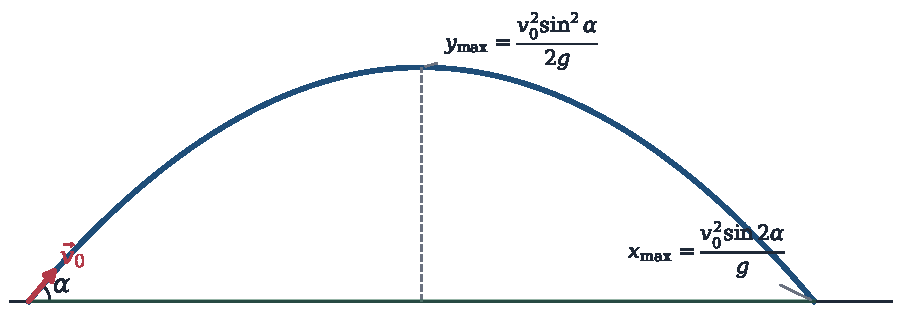
\includegraphics[width=0.78\textwidth]{figures/06_projectile.pdf}
\caption{Parabolic projectile trajectory launched with speed $v_0$ at angle $\alpha$. Velocity vectors $\vec{v}(t)$ remain tangent to the curve, while acceleration $\vec{a} = -g\jhat$ is constant throughout.}
\label{fig:projectile}
\end{figure}

A projectile launched from origin $(0,0)$ with initial speed $v_0$ at launch angle $\alpha$ subject only to uniform gravity $\vec{g} = -g\jhat$ satisfies:
\[
\ddot{x}(t) = 0, \qquad \ddot{y}(t) = -g.
\]
Integrating with initial velocity $\vec{v}_0 = v_0\cos\alpha\,\ihat + v_0\sin\alpha\,\jhat$:
\begin{align*}
v_x(t) &= v_0\cos\alpha = \text{const}, \qquad & x(t) &= v_0\cos\alpha\,t, \\
v_y(t) &= v_0\sin\alpha - gt, \qquad & y(t) &= v_0\sin\alpha\,t - \frac{1}{2}gt^2.
\end{align*}
Eliminating $t = \frac{x}{v_0\cos\alpha}$ yields the \textbf{Cartesian trajectory}:
\[
\boxed{y(x) = x\tan\alpha - \frac{g}{2v_0^2\cos^2\alpha}x^2.}
\]
Since $1/\cos^2\alpha = 1 + \tan^2\alpha$, this can be written as:
\[
\boxed{y(x) = x\tan\alpha - \frac{g x^2}{2v_0^2}\left(1 + \tan^2\alpha\right).}
\]
This is a parabola opening downwards with vertex at:
\[
x_H = \frac{v_0^2\sin(2\alpha)}{2g}, \qquad H_{\max} = \frac{v_0^2\sin^2\alpha}{2g}.
\]
The horizontal range $R$ on level ground ($y = 0, x \ne 0$) is:
\[
\boxed{R = \frac{v_0^2\sin(2\alpha)}{g}.}
\]
\begin{itemize}[leftmargin=1.4em,itemsep=2pt]
  \item Maximum range occurs at $\alpha = 45^\circ$, where $R_{\max} = \frac{v_0^2}{g}$.
  \item Complementary launch angles $\alpha$ and $90^\circ - \alpha$ yield identical horizontal ranges, since $\sin(2(90^\circ - \alpha)) = \sin(180^\circ - 2\alpha) = \sin(2\alpha)$.
\end{itemize}

\section{Circular Motion and Kinematics of Rotation}

\begin{figure}[htbp]
\centering
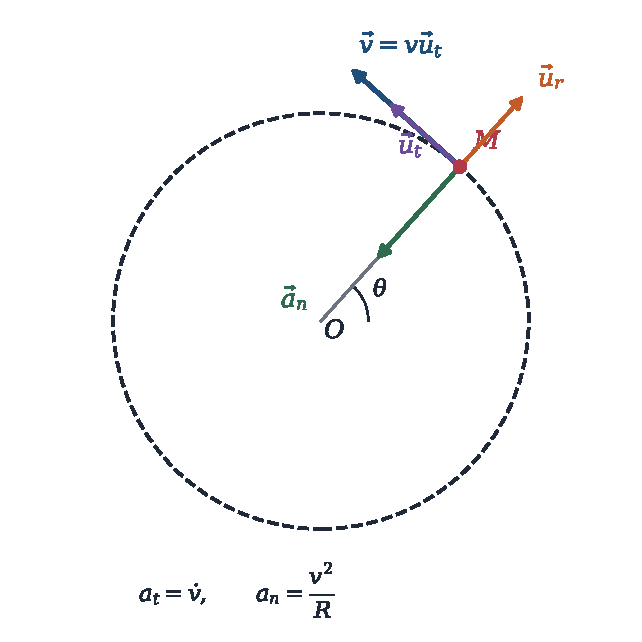
\includegraphics[width=0.74\textwidth]{figures/07_circular_motion.pdf}
\caption{Uniform circular motion of radius $R$. The velocity is strictly tangential $\vec{v} = v\ut$, while the acceleration is purely centripetal $\vec{a} = -\frac{v^2}{R}\ur = -\omega^2 R\ur$.}
\label{fig:circular_motion}
\end{figure}

For a particle moving on a circle of radius $R$, its position is specified by angular coordinate $\theta(t)$:
\[
\vec{r}(t) = R\cos\theta(t)\,\ihat + R\sin\theta(t)\,\jhat.
\]
Differentiating with respect to time:
\[
\vec{v}(t) = R\dot{\theta}\left( -\sin\theta\,\ihat + \cos\theta\,\jhat \right) = R\omega\,\ut,
\]
where $\omega = \dot{\theta} = \frac{\dd\theta}{\dd t}$ is the \textbf{angular velocity} (in $\mathrm{rad\,s^{-1}}$), and linear speed is $v = R\omega$.

Differentiating once more yields the acceleration:
\[
\vec{a}(t) = \frac{\dd}{\dd t}(R\omega\ut) = R\dot{\omega}\,\ut + R\omega\frac{\dd\ut}{\dd t} = R\alpha\,\ut + R\omega(-\omega\ur),
\]
where $\alpha = \dot{\omega} = \ddot{\theta}$ is the \textbf{angular acceleration}.
Thus, the acceleration cleanly splits into two perpendicular components:
\[
\boxed{\vec{a} = \vec{a}_t + \vec{a}_n = R\alpha\,\ut - \omega^2 R\,\ur = R\ddot{\theta}\,\ut - \frac{v^2}{R}\ur.}
\]
\begin{itemize}[leftmargin=1.4em,itemsep=2pt]
  \item The \textbf{tangential acceleration} $a_t = R\alpha = \frac{\dd v}{\dd t}$ changes the \emph{speed} (rate of motion).
  \item The \textbf{centripetal (normal) acceleration} $a_n = \frac{v^2}{R} = \omega^2 R$ points toward the center of curvature and changes the \emph{direction} of the velocity vector.
\end{itemize}

\section{Extensive Worked Examples}

\begin{workedexample}{The Parabola of Safety (Envelope of All Trajectories)}
A coastal defense battery fires shells at a fixed muzzle speed $v_0$, but can vary the launch angle $\alpha \in [0, \pi/2]$ arbitrarily in the vertical plane.
Find the boundary curve in the $(x, y)$ plane that separates points that can be hit by shells from points that are safe from bombardment.

\paragraph{Solution.}

A target at coordinates $(x, y)$ can be hit if and only if there exists at least one real physical launch angle $\alpha$ whose trajectory passes through $(x, y)$.
Recall the trajectory equation expressed in terms of $T \equiv \tan\alpha$:
\[
y = x T - \frac{gx^2}{2v_0^2}(1 + T^2).
\]
Multiply by $\frac{2v_0^2}{gx^2}$ and rearrange into standard quadratic form for $T$:
\[
\frac{gx^2}{2v_0^2}T^2 - x T + \left(y + \frac{gx^2}{2v_0^2}\right) = 0.
\]
This is a quadratic equation $A T^2 + B T + C = 0$ in the unknown $T = \tan\alpha$, with coefficients:
\[
A = \frac{gx^2}{2v_0^2}, \qquad B = -x, \qquad C = y + \frac{gx^2}{2v_0^2}.
\]
Real physical solutions for launch angle $\alpha$ exist if and only if the discriminant $\Delta$ is non-negative:
\[
\Delta = B^2 - 4AC \ge 0.
\]
Evaluating the discriminant:
\[
\Delta = (-x)^2 - 4\left(\frac{gx^2}{2v_0^2}\right)\left(y + \frac{gx^2}{2v_0^2}\right) = x^2 - \frac{2gx^2}{v_0^2}y - \left(\frac{gx^2}{v_0^2}\right)^2 \ge 0.
\]
Dividing by $x^2 > 0$:
\[
1 - \frac{2gy}{v_0^2} - \frac{g^2 x^2}{v_0^4} \ge 0 \implies \frac{2gy}{v_0^2} \le 1 - \frac{g^2 x^2}{v_0^4}.
\]
Multiplying by $\frac{v_0^2}{2g}$:
\[
\boxed{y \le \frac{v_0^2}{2g} - \frac{g}{2v_0^2}x^2.}
\]
The boundary separating hit points ($\Delta > 0$, where two distinct trajectory angles exist: low trajectory and high lob trajectory) from unreachable points ($\Delta < 0$) is the \textbf{Parabola of Safety}:
\[
\boxed{y_{\text{safety}}(x) = H_0 - \frac{x^2}{4H_0}, \quad \text{where } H_0 = \frac{v_0^2}{2g}.}
\]
Every point outside this bounding paraboloid of revolution is completely immune to bombardment.
\end{workedexample}

\begin{workedexample}{Projectile Range on an Inclined Plane}
A projectile is fired with speed $v_0$ at angle $\alpha$ above the horizontal onto a hillside that slopes upward at a constant angle $\beta < \alpha$.
(a) Find the flight time $t_f$ until the projectile strikes the hill.
(b) Calculate the distance $d(\alpha)$ measured along the slope of the hill.
(c) Find the optimal launch angle $\alpha_{\text{opt}}$ that maximizes $d$, and find the maximum range along the incline.

\paragraph{Solution.}

(a) Align a tilted coordinate frame with the $x'$-axis pointing up the incline (angle $\beta$) and $y'$-axis normal to the incline.
In this tilted frame:
\begin{itemize}[leftmargin=1.4em,itemsep=2pt]
  \item Gravity components: $g_{x'} = -g\sin\beta$, $g_{y'} = -g\cos\beta$.
  \item Launch angle relative to incline: $\theta_0 = \alpha - \beta$.
  \item Initial velocity: $v_{x'0} = v_0\cos(\alpha - \beta)$, $v_{y'0} = v_0\sin(\alpha - \beta)$.
\end{itemize}
The motion perpendicular to the incline is:
\[
y'(t) = v_0\sin(\alpha - \beta)t - \frac{1}{2}g\cos\beta\,t^2.
\]
Impact occurs when $y'(t_f) = 0$ ($t_f \ne 0$):
\[
\boxed{t_f = \frac{2v_0\sin(\alpha - \beta)}{g\cos\beta}.}
\]

(b) The distance along the incline is $d = x'(t_f)$:
\[
x'(t) = v_0\cos(\alpha - \beta)t - \frac{1}{2}g\sin\beta\,t^2.
\]
Substituting $t_f$:
\begin{align*}
d &= v_0\cos(\alpha - \beta)\left(\frac{2v_0\sin(\alpha - \beta)}{g\cos\beta}\right) - \frac{1}{2}g\sin\beta\left(\frac{2v_0\sin(\alpha - \beta)}{g\cos\beta}\right)^2 \\
&= \frac{2v_0^2\sin(\alpha - \beta)}{g\cos^2\beta}\left[ \cos(\alpha - \beta)\cos\beta - \sin(\alpha - \beta)\sin\beta \right].
\end{align*}
Using the angle addition identity $\cos(A+B) = \cos A\cos B - \sin A\sin B$ with $A = \alpha - \beta$ and $B = \beta$:
\[
\cos(\alpha - \beta)\cos\beta - \sin(\alpha - \beta)\sin\beta = \cos((\alpha - \beta) + \beta) = \cos\alpha.
\]
Thus:
\[
\boxed{d(\alpha) = \frac{2v_0^2}{g\cos^2\beta}\sin(\alpha - \beta)\cos\alpha.}
\]
Using product-to-sum: $2\sin A\cos B = \sin(A+B) + \sin(A-B)$:
\[
2\sin(\alpha - \beta)\cos\alpha = \sin(2\alpha - \beta) - \sin\beta.
\]
Therefore:
\[
\boxed{d(\alpha) = \frac{v_0^2}{g\cos^2\beta}\left[ \sin(2\alpha - \beta) - \sin\beta \right].}
\]

(c) Since $\beta$ is fixed, $d(\alpha)$ is maximized when $\sin(2\alpha - \beta) = 1$:
\[
2\alpha_{\text{opt}} - \beta = 90^\circ \implies \boxed{\alpha_{\text{opt}} = 45^\circ + \frac{\beta}{2}.}
\]
The optimal launch angle bisects the angle between the incline and the vertical!
The maximum range along the incline is:
\[
d_{\max} = \frac{v_0^2}{g\cos^2\beta}(1 - \sin\beta) = \frac{v_0^2(1 - \sin\beta)}{g(1 - \sin^2\beta)} = \frac{v_0^2(1 - \sin\beta)}{g(1 - \sin\beta)(1 + \sin\beta)} = \boxed{\frac{v_0^2}{g(1 + \sin\beta)}.}
\]
For flat ground ($\beta = 0$), this recovers $\alpha_{\text{opt}} = 45^\circ$ and $d_{\max} = v_0^2/g$.
\end{workedexample}

\begin{workedexample}{The Velocity Hodograph of Projectile Motion}
The \textbf{hodograph} of a motion is the trajectory traced by the tip of the velocity vector $\vec{v}(t)$ in velocity space with coordinates $(v_x, v_y)$.
(a) For a projectile in gravity $\vec{g} = -g\jhat$, sketch the hodograph.
(b) Show that the hodograph is a vertical straight line traversed at constant speed.
(c) Deduce that for any motion with constant acceleration $\vec{a}_0$, the hodograph is a straight line along $\vec{a}_0$.

\paragraph{Solution.}

(a) The velocity vector of a projectile is:
\[
v_x(t) = v_0\cos\alpha = \text{const}, \qquad v_y(t) = v_0\sin\alpha - gt.
\]
In the velocity plane $(v_x, v_y)$, the $v_x$ coordinate never changes ($v_x \equiv v_{x0}$), while the $v_y$ coordinate decreases linearly with time.
Thus, the hodograph is a \textbf{vertical straight line} at distance $v_x = v_0\cos\alpha$ from the $v_y$-axis.

(b) The position vector in velocity space is $\vec{v}(t)$. Its velocity of transit along the hodograph is:
\[
\vec{w}_{\text{hodograph}} = \frac{\dd\vec{v}}{\dd t} = \vec{a}(t) = -g\jhat.
\]
The speed of travel along the hodograph line is constant and equals the gravitational acceleration:
\[
\norm{\vec{w}} = g = 9.81\ \mathrm{m\,s^{-2}} = \text{constant.}
\]

(c) In general, for any particle under constant acceleration $\vec{a}_0$:
\[
\vec{v}(t) = \vec{v}_0 + \vec{a}_0 t.
\]
This is the parametric vector equation of a straight line in velocity space passing through $\vec{v}_0$ parallel to $\vec{a}_0$, traversed with uniform speed $\norm{\vec{a}_0}$. Sir William Rowan Hamilton originally used the hodograph to discover that the velocity locus of planetary orbits is an exact circle!
\end{workedexample}

\chapter{Curvilinear Coordinates and Intrinsic Frames}
\label{ch:curvilinear}

\begin{chapterintro}
\textbf{Chapter Objectives:} When trajectories exhibit natural geometric symmetries, Cartesian coordinates become cumbersome. In this chapter, you will master the intrinsic Frenet-Serret frame $(\vec{u}_t, \vec{u}_n, \vec{u}_b)$; calculate radii of curvature; and derive the fundamental velocity and acceleration vectors in plane polar, cylindrical, and spherical coordinates.
\end{chapterintro}

\section{The Intrinsic Frame of Frenet-Serret}

\begin{figure}[htbp]
\centering
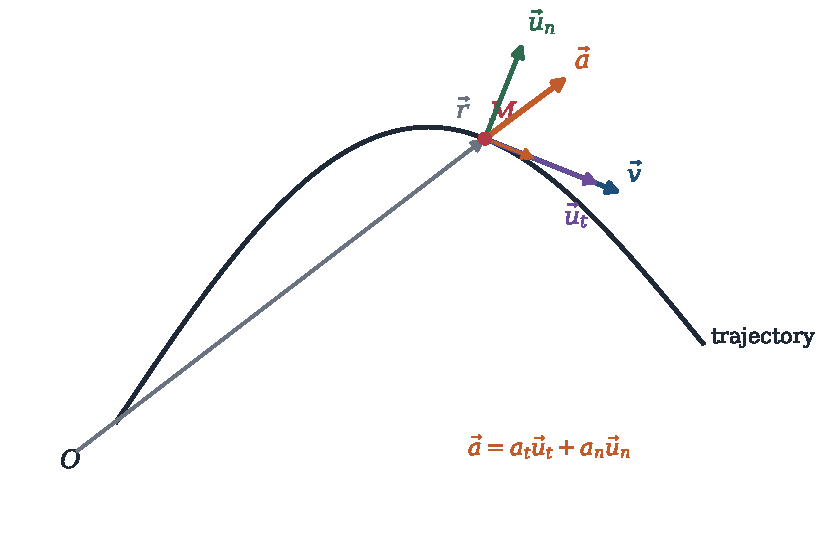
\includegraphics[width=0.74\textwidth]{figures/04_trajectory_frame.pdf}
\caption{The intrinsic Frenet-Serret frame moving along a curved trajectory. Tangent unit vector $\vec{u}_t$ is collinear with velocity, while normal unit vector $\vec{u}_n$ points toward the center of curvature.}
\label{fig:trajectory_frame}
\end{figure}

Let a trajectory curve $\mathcal{C}$ be parametrized by its \textbf{curvilinear abscissa (arc length)} $s(t)$ measured from a reference point $A$:
\[
\dd s = \norm{\dd\vec{r}} = \sqrt{\dd x^2 + \dd y^2 + \dd z^2}.
\]
At any regular point on $\mathcal{C}$, the local moving orthonormal \textbf{Frenet-Serret frame} $(\vec{u}_t, \vec{u}_n, \vec{u}_b)$ is constructed as follows:
\begin{enumerate}[leftmargin=1.5em,itemsep=3pt]
  \item \textbf{Unit Tangent Vector $\vec{u}_t$}:
        \[
        \boxed{\vec{u}_t = \frac{\dd\vec{r}}{\dd s} = \frac{\dd\vec{r}/\dd t}{\dd s/\dd t} = \frac{\vec{v}}{v}.}
        \]
        The velocity is always purely tangential: $\vec{v}(t) = v(t)\,\vec{u}_t$.
  \item \textbf{Unit Principal Normal $\vec{u}_n$ and Radius of Curvature $R$}:
        Since $\vec{u}_t\cdot\vec{u}_t = 1$, its spatial derivative $\frac{\dd\vec{u}_t}{\dd s}$ is strictly orthogonal to $\vec{u}_t$. The \textbf{curvature} $\kappa = 1/R$ and unit principal normal $\vec{u}_n$ are defined by:
        \[
        \boxed{\frac{\dd\vec{u}_t}{\dd s} = \kappa\,\vec{u}_n = \frac{1}{R}\,\vec{u}_n,}
        \]
        where $R$ is the local \textbf{radius of curvature} of the trajectory and $\vec{u}_n$ points into the concave side toward the center of curvature.
  \item \textbf{Unit Binormal Vector $\vec{u}_b$}:
        \[
        \vec{u}_b = \vec{u}_t\times\vec{u}_n.
        \]
\end{enumerate}

\begin{lawbox}{Acceleration in the Frenet-Serret Frame}
Differentiating the velocity $\vec{v} = v\,\vec{u}_t$ with respect to time using the chain rule $\frac{\dd\vec{u}_t}{\dd t} = \frac{\dd s}{\dd t}\frac{\dd\vec{u}_t}{\dd s} = v\left(\frac{1}{R}\vec{u}_n\right)$:
\[
\vec{a}(t) = \frac{\dd}{\dd t}\left(v\,\vec{u}_t\right) = \frac{\dd v}{\dd t}\vec{u}_t + v\frac{\dd\vec{u}_t}{\dd t} = \frac{\dd v}{\dd t}\vec{u}_t + v\left(v\frac{1}{R}\vec{u}_n\right).
\]
Therefore:
\[
\boxed{\vec{a} = a_t\,\vec{u}_t + a_n\,\vec{u}_n = \frac{\dd v}{\dd t}\vec{u}_t + \frac{v^2}{R}\vec{u}_n.}
\]
Notice that the binormal component of acceleration is identically zero ($a_b \equiv 0$); acceleration always lies in the \textbf{osculating plane} spanned by $\vec{u}_t$ and $\vec{u}_n$.
\end{lawbox}

\section{Plane Polar Coordinates $(r, \theta)$}

\begin{figure}[htbp]
\centering
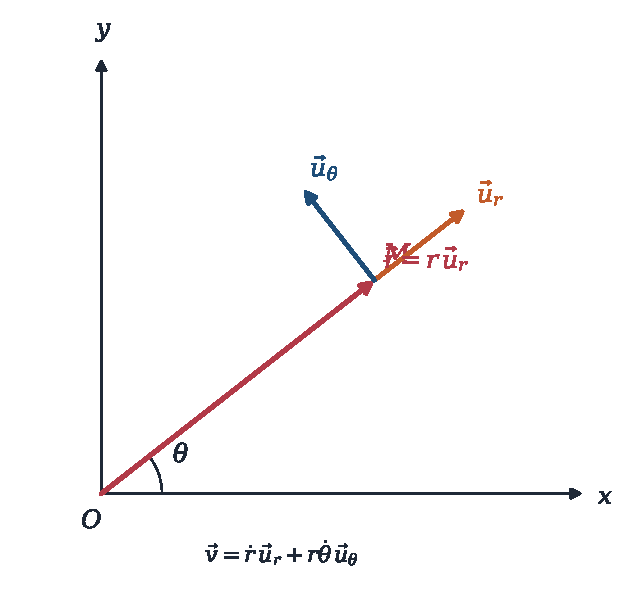
\includegraphics[width=0.74\textwidth]{figures/08_polar_basis.pdf}
\caption{Plane polar basis $(\ur, \ut)$. As the polar angle $\theta$ changes, the unit vectors rotate according to $\dot{\ur} = \dot{\theta}\ut$ and $\dot{\ut} = -\dot{\theta}\ur$.}
\label{fig:polar_basis}
\end{figure}

The position of a particle in the $xy$-plane is specified by radial distance $r = \norm{\vec{OM}}$ and polar angle $\theta$ measured counterclockwise from the positive $x$-axis:
\[
x = r\cos\theta, \qquad y = r\sin\theta.
\]
The orthonormal basis vectors are:
\[
\ur = \cos\theta\,\ihat + \sin\theta\,\jhat, \qquad \ut = -\sin\theta\,\ihat + \cos\theta\,\jhat.
\]
Differentiating with respect to time:
\[
\boxed{\frac{\dd\ur}{\dd t} = \dot{\theta}\,\ut}, \qquad \boxed{\frac{\dd\ut}{\dd t} = -\dot{\theta}\,\ur.}
\]

\begin{lawbox}{Kinematics in Plane Polar Coordinates}
\begin{itemize}[leftmargin=1.4em,itemsep=3pt]
  \item \textbf{Position}:
        \[
        \vec{r} = r\,\ur.
        \]
  \item \textbf{Velocity}:
        \[
        \boxed{\vec{v} = \dot{r}\,\ur + r\dot{\theta}\,\ut = v_r\,\ur + v_\theta\,\ut.}
        \]
  \item \textbf{Acceleration}:
        Differentiating $\vec{v}$:
        \[
        \vec{a} = \ddot{r}\ur + \dot{r}(\dot{\theta}\ut) + \dot{r}\dot{\theta}\ut + r\ddot{\theta}\ut + r\dot{\theta}(-\dot{\theta}\ur).
        \]
        Grouping components:
        \[
        \boxed{\vec{a} = (\ddot{r} - r\dot{\theta}^2)\ur + (r\ddot{\theta} + 2\dot{r}\dot{\theta})\ut = a_r\,\ur + a_\theta\,\ut.}
        \]
        Notice that the transverse component can be written compactly as:
        \[
        \boxed{a_\theta = \frac{1}{r}\frac{\dd}{\dd t}\left(r^2\dot{\theta}\right).}
        \]
        The term $-r\dot{\theta}^2$ is the centripetal acceleration, while $2\dot{r}\dot{\theta}$ is the kinematic \textbf{Coriolis term} in polar coordinates.
\end{itemize}
\end{lawbox}

\section{Cylindrical and Spherical Coordinates}

\begin{figure}[htbp]
\centering
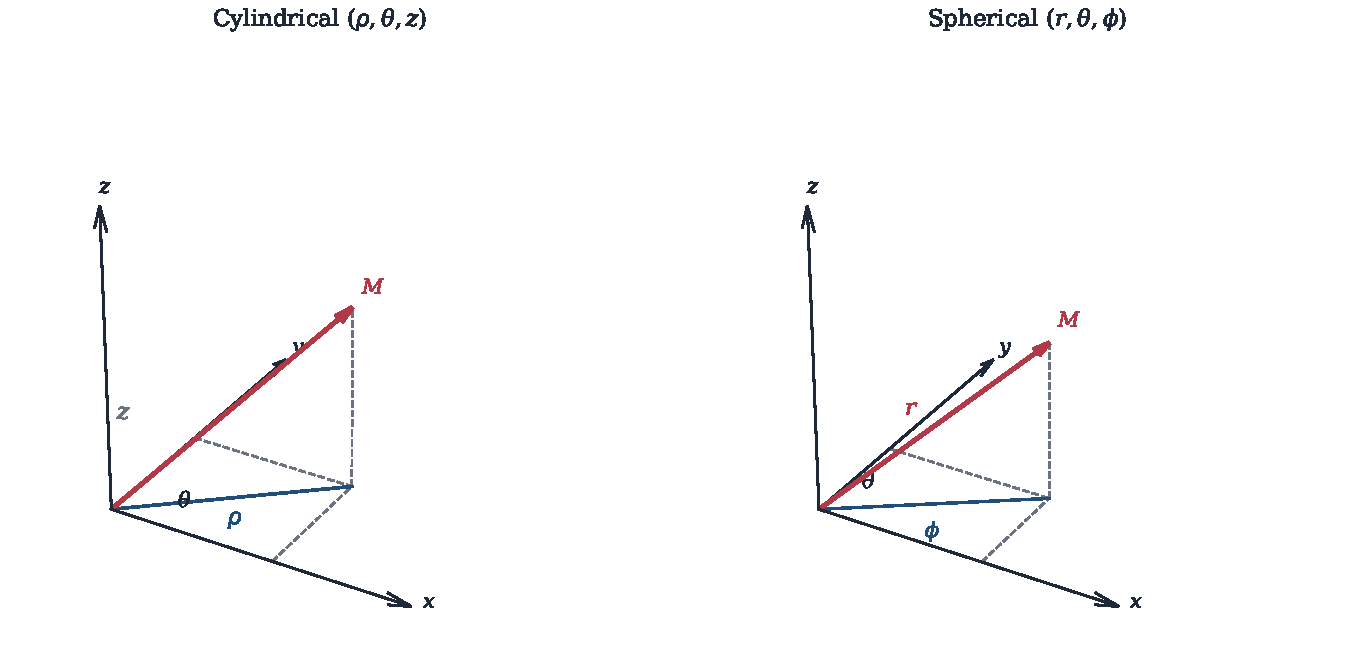
\includegraphics[width=0.82\textwidth]{figures/09_cyl_spherical.pdf}
\caption{Cylindrical coordinates $(\rho, \theta, z)$ and Spherical coordinates $(r, \theta, \phi)$ with their respective local moving coordinate frames.}
\label{fig:cyl_spherical}
\end{figure}

\subsection{Cylindrical Coordinates $(\rho, \theta, z)$}
\begin{align*}
\vec{r} &= \rho\,\vec{u}_\rho + z\,\khat, \\
\vec{v} &= \dot{\rho}\,\vec{u}_\rho + \rho\dot{\theta}\,\ut + \dot{z}\,\khat, \\
\vec{a} &= (\ddot{\rho} - \rho\dot{\theta}^2)\vec{u}_\rho + \frac{1}{\rho}\frac{\dd(\rho^2\dot{\theta})}{\dd t}\ut + \ddot{z}\,\khat.
\end{align*}

\subsection{Spherical Coordinates $(r, \theta, \phi)$}
Here $r \ge 0$ is the radial distance, $\theta \in [0, \pi]$ is the colatitude (polar angle from $+z$), and $\phi \in [0, 2\pi)$ is the azimuthal angle:
\[
x = r\sin\theta\cos\phi, \qquad y = r\sin\theta\sin\phi, \qquad z = r\cos\theta.
\]
The velocity vector is:
\[
\boxed{\vec{v} = \dot{r}\,\ur + r\dot{\theta}\,\ut + r\sin\theta\dot{\phi}\,\uphi.}
\]
The acceleration vector components are:
\begin{align}
a_r &= \ddot{r} - r\dot{\theta}^2 - r\sin^2\theta\dot{\phi}^2, \\
a_\theta &= r\ddot{\theta} + 2\dot{r}\dot{\theta} - r\sin\theta\cos\theta\dot{\phi}^2, \\
a_\phi &= r\sin\theta\ddot{\phi} + 2\sin\theta\dot{r}\dot{\phi} + 2r\cos\theta\dot{\theta}\dot{\phi} = \frac{1}{r\sin\theta}\frac{\dd}{\dd t}\left(r^2\sin^2\theta\dot{\phi}\right).
\end{align}

\section{Extensive Worked Examples}

\begin{workedexample}{Radius of Curvature of a Parabolic Projectile Path}
For a projectile fired with speed $v_0$ at angle $\alpha$, the acceleration is $\vec{a} = -g\jhat$ everywhere.
(a) At the highest point (apex) of the trajectory, find the speed $v_{\text{apex}}$ and the radius of curvature $R_{\text{apex}}$.
(b) At the launch point $(0,0)$, find the tangential acceleration $a_t$ and the radius of curvature $R_{\text{launch}}$.
(c) Deduce the general formula for the radius of curvature $R(t)$ at any instant $t$.

\paragraph{Solution.}

(a) At the apex, the vertical velocity is zero ($v_y = 0$). The velocity is purely horizontal:
\[
\vec{v}_{\text{apex}} = (v_0\cos\alpha)\ihat \implies v_{\text{apex}} = v_0\cos\alpha.
\]
Since velocity is horizontal, the unit tangent is $\vec{u}_t = \ihat$.
The acceleration is purely vertical: $\vec{a} = -g\jhat$.
Because $\vec{a}\perp\vec{v}$, the tangential acceleration is zero: $a_t = 0$.
The entire acceleration is normal (centripetal):
\[
a_n = g.
\]
From the Frenet acceleration relation $a_n = \frac{v^2}{R}$:
\[
g = \frac{v_{\text{apex}}^2}{R_{\text{apex}}} \implies \boxed{R_{\text{apex}} = \frac{v_{\text{apex}}^2}{g} = \frac{v_0^2\cos^2\alpha}{g}.}
\]

(b) At the launch point:
The initial velocity is $\vec{v}_0 = v_0\cos\alpha\,\ihat + v_0\sin\alpha\,\jhat$, with speed $v_0$.
The unit tangent vector is:
\[
\vec{u}_t = \cos\alpha\,\ihat + \sin\alpha\,\jhat.
\]
The tangential acceleration is the projection of $\vec{a} = -g\jhat$ onto $\vec{u}_t$:
\[
a_t = \vec{a}\cdot\vec{u}_t = (-g\jhat)\cdot(\cos\alpha\,\ihat + \sin\alpha\,\jhat) = \boxed{-g\sin\alpha.}
\]
The normal acceleration is obtained from $a^2 = a_t^2 + a_n^2$:
\[
a_n = \sqrt{a^2 - a_t^2} = \sqrt{g^2 - (-g\sin\alpha)^2} = g\sqrt{1 - \sin^2\alpha} = \boxed{g\cos\alpha.}
\]
The radius of curvature at launch is:
\[
a_n = \frac{v_0^2}{R_{\text{launch}}} \implies \boxed{R_{\text{launch}} = \frac{v_0^2}{a_n} = \frac{v_0^2}{g\cos\alpha}.}
\]

(c) At any arbitrary instant $t$:
The speed is $v(t) = \sqrt{(v_0\cos\alpha)^2 + (v_0\sin\alpha - gt)^2}$.
The cross product $\norm{\vec{v}\times\vec{a}}$ provides an elegant shortcut:
\[
\vec{v}\times\vec{a} = (v_x\ihat + v_y\jhat)\times(-g\jhat) = -g v_x\,\khat \implies \norm{\vec{v}\times\vec{a}} = g v_x = g v_0\cos\alpha.
\]
On the other hand, in the Frenet frame $\vec{v} = v\vec{u}_t$ and $\vec{a} = a_t\vec{u}_t + a_n\vec{u}_n$:
\[
\norm{\vec{v}\times\vec{a}} = \norm{v\vec{u}_t\times(a_t\vec{u}_t + a_n\vec{u}_n)} = v a_n = v\left(\frac{v^2}{R}\right) = \frac{v^3}{R}.
\]
Equating the two expressions:
\[
\frac{v^3}{R} = g v_0\cos\alpha \implies \boxed{R(t) = \frac{v^3(t)}{g v_0\cos\alpha} = \frac{\left[ (v_0\cos\alpha)^2 + (v_0\sin\alpha - gt)^2 \right]^{3/2}}{g v_0\cos\alpha}.}
\]
At $t = 0$, $R(0) = \frac{v_0^3}{g v_0\cos\alpha} = \frac{v_0^2}{g\cos\alpha}$; at apex ($v_y = 0$), $R = \frac{(v_0\cos\alpha)^3}{g v_0\cos\alpha} = \frac{v_0^2\cos^2\alpha}{g}$. Exact agreement!
\end{workedexample}

\begin{workedexample}{Particle Moving on a Circular Helix}
A particle moves along a vertical circular helix of radius $R$ and pitch $2\pi h$ according to:
\[
\vec{r}(t) = R\cos(\omega t)\,\ihat + R\sin(\omega t)\,\jhat + (c\omega t)\,\khat,
\]
where $\omega$ and $c$ are positive constants.
(a) Find the velocity vector $\vec{v}(t)$ and speed $v$.
(b) Determine the Frenet unit vectors $\vec{u}_t, \vec{u}_n, \vec{u}_b$.
(c) Calculate the radius of curvature $R_c$ and the torsion $\tau$ of the helix.

\paragraph{Solution.}

(a) Differentiating position with respect to time:
\[
\vec{v}(t) = \dot{\vec{r}}(t) = -R\omega\sin(\omega t)\,\ihat + R\omega\cos(\omega t)\,\jhat + c\omega\,\khat.
\]
The speed is constant:
\[
\boxed{v = \norm{\vec{v}} = \sqrt{(-R\omega\sin\omega t)^2 + (R\omega\cos\omega t)^2 + (c\omega)^2} = \omega\sqrt{R^2 + c^2} = \text{const}.}
\]

(b) Frenet vectors:
\begin{itemize}[leftmargin=1.4em,itemsep=2pt]
  \item Unit tangent:
  \[
  \vec{u}_t = \frac{\vec{v}}{v} = \frac{1}{\sqrt{R^2 + c^2}}\left[ -R\sin(\omega t)\,\ihat + R\cos(\omega t)\,\jhat + c\,\khat \right].
  \]
  \item Acceleration:
  \[
  \vec{a}(t) = \dot{\vec{v}}(t) = -R\omega^2\cos(\omega t)\,\ihat - R\omega^2\sin(\omega t)\,\jhat + 0\,\khat = -R\omega^2\left[ \cos(\omega t)\,\ihat + \sin(\omega t)\,\jhat \right].
  \]
  Since speed is constant ($v = \text{const}$), the tangential acceleration is zero: $a_t = \dot{v} = 0$.
  Thus $\vec{a} = a_n\vec{u}_n$. Since $\norm{\vec{a}} = R\omega^2$, the unit principal normal is:
  \[
  \vec{u}_n = \frac{\vec{a}}{\norm{\vec{a}}} = \boxed{-\cos(\omega t)\,\ihat - \sin(\omega t)\,\jhat.}
  \]
  The principal normal points horizontally directly toward the central axis of the cylinder!
  \item Unit binormal:
  \begin{align*}
  \vec{u}_b &= \vec{u}_t\times\vec{u}_n = \frac{1}{\sqrt{R^2 + c^2}}\begin{vmatrix} \ihat & \jhat & \khat \\ -R\sin\omega t & R\cos\omega t & c \\ -\cos\omega t & -\sin\omega t & 0 \end{vmatrix} \\
  &= \frac{1}{\sqrt{R^2 + c^2}}\left[ c\sin(\omega t)\,\ihat - c\cos(\omega t)\,\jhat + (R\sin^2\omega t + R\cos^2\omega t)\khat \right] \\
  &= \boxed{\frac{1}{\sqrt{R^2 + c^2}}\left[ c\sin(\omega t)\,\ihat - c\cos(\omega t)\,\jhat + R\,\khat \right].}
  \end{align*}
\end{itemize}

(c) Curvature and radius of curvature:
\[
a_n = \frac{v^2}{R_c} \implies R\omega^2 = \frac{\omega^2(R^2 + c^2)}{R_c} \implies \boxed{R_c = \frac{R^2 + c^2}{R} = R\left(1 + \frac{c^2}{R^2}\right).}
\]
Notice that $R_c > R$: the curvature of a helix is always strictly less than the curvature of its base circle!

For torsion $\tau$: from the third Frenet-Serret formula $\frac{\dd\vec{u}_b}{\dd s} = -\tau\vec{u}_n$:
\[
\frac{\dd\vec{u}_b}{\dd t} = \frac{c\omega}{\sqrt{R^2 + c^2}}\left[ \cos(\omega t)\,\ihat + \sin(\omega t)\,\jhat \right] = -\frac{c\omega}{\sqrt{R^2 + c^2}}\vec{u}_n.
\]
Since $\frac{\dd\vec{u}_b}{\dd t} = v\frac{\dd\vec{u}_b}{\dd s} = -v\tau\vec{u}_n$:
\[
v\tau = \frac{c\omega}{\sqrt{R^2 + c^2}} \implies \left(\omega\sqrt{R^2 + c^2}\right)\tau = \frac{c\omega}{\sqrt{R^2 + c^2}} \implies \boxed{\tau = \frac{c}{R^2 + c^2}.}
\]
Both the curvature and the torsion of a circular helix are constant everywhere along its length.
\end{workedexample}

\chapter{Relative Motion and Kinematics in Moving Frames}
\label{ch:relative}

\begin{chapterintro}
\textbf{Chapter Objectives:} All motion in physics is relative to an observer's frame of reference. In this chapter, you will master the operator relation connecting time derivatives between fixed and rotating frames; prove the classical laws of velocity and acceleration composition; and unveil the kinematic origin of the Coriolis acceleration $2\vec{\Omega}\times\vec{v}_r$.
\end{chapterintro}

\section{Reference Frames and the Moving Basis}

Let $\mathcal{R}(O, \ihat, \jhat, \khat)$ be a reference frame assumed fixed (inertial), and let $\mathcal{R}'(O', \ihat', \jhat', \khat')$ be a secondary reference frame moving with respect to $\mathcal{R}$.
The motion of $\mathcal{R}'$ relative to $\mathcal{R}$ is completely specified by:
\begin{enumerate}[leftmargin=1.5em,itemsep=2pt]
  \item The translational position and velocity of its origin: $\vec{OO'}(t)$ and $\vec{v}_{\mathcal{R}}(O') = \left(\frac{\dd\vec{OO'}}{\dd t}\right)_{\mathcal{R}}$.
  \item Its instantaneous \textbf{angular velocity vector} $\vec{\Omega}_{\mathcal{R}'/\mathcal{R}}(t)$ characterizing the rotation of its basis vectors $(\ihat', \jhat', \khat')$.
\end{enumerate}

\begin{figure}[htbp]
\centering
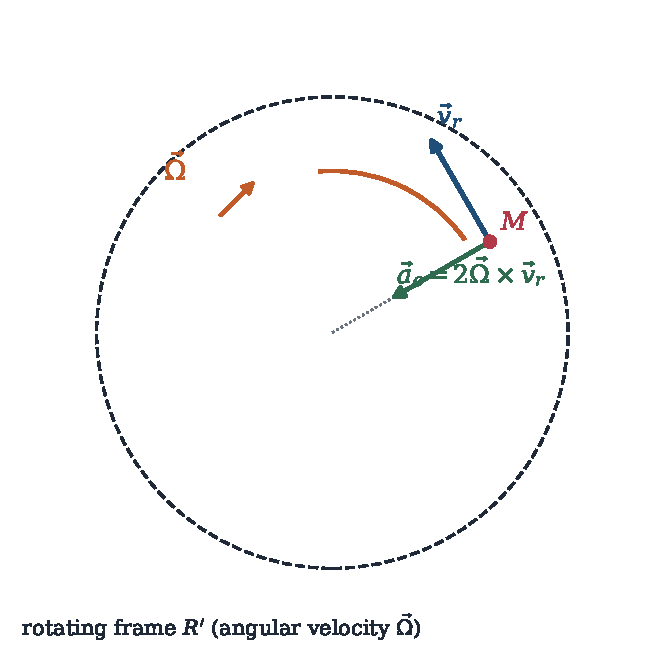
\includegraphics[width=0.74\textwidth]{figures/10_rotating_frame.pdf}
\caption{A particle $M$ observed from both a fixed frame $\mathcal{R}$ and a moving rotating frame $\mathcal{R}'$ with angular velocity $\vec{\Omega}$.}
\label{fig:relative_frame}
\end{figure}

\begin{historicalbox}{Gaspard-Gustave de Coriolis (1792--1843)}
\begin{minipage}{0.28\textwidth}
\centering
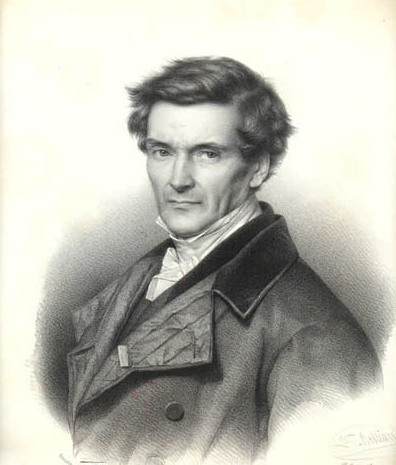
\includegraphics[width=0.95\textwidth]{images/coriolis.jpg}
\captionof{figure}{Gaspard-Gustave de Coriolis (1792--1843), French mathematician and mechanical engineer.}
\end{minipage}\hfill
\begin{minipage}{0.68\textwidth}
Trained at the École Polytechnique, Coriolis was investigating the efficiency of waterwheels, rotating turbines, and mechanical engines with spinning components when he published his landmark 1835 paper \emph{``Sur les équations du mouvement relatif des systèmes de corps''}.

Coriolis demonstrated mathematically that an observer located on a rotating platform detects a subtle supplementary acceleration $2\vec{\Omega}\times\vec{v}_r$ acting on any moving object. Though originally derived for industrial machinery, the Coriolis acceleration became the key to understanding global meteorology, trade winds, cyclonic storms, and oceanic currents.
\end{minipage}
\end{historicalbox}

\section{The Fundamental Kinematic Derivative Operator}

Let $\vec{A}(t) = A_x'\ihat' + A_y'\jhat' + A_z'\khat'$ be an arbitrary vector.
Its time derivative as evaluated by an observer stationary in $\mathcal{R}'$ is:
\[
\left(\frac{\dd\vec{A}}{\dd t}\right)_{\mathcal{R}'} \equiv \dot{A}_x'\ihat' + \dot{A}_y'\jhat' + \dot{A}_z'\khat'.
\]
However, for an observer in $\mathcal{R}$, the basis vectors $(\ihat', \jhat', \khat')$ also rotate according to Poisson's relation $\dot{\vec{u}}' = \vec{\Omega}\times\vec{u}'$:
\[
\left(\frac{\dd\vec{A}}{\dd t}\right)_{\mathcal{R}} = \left(\dot{A}_x'\ihat' + \dot{A}_y'\jhat' + \dot{A}_z'\khat'\right) + \left(A_x'\frac{\dd\ihat'}{\dd t} + A_y'\frac{\dd\jhat'}{\dd t} + A_z'\frac{\dd\khat'}{\dd t}\right).
\]
Substituting $\frac{\dd\vec{u}'}{\dd t} = \vec{\Omega}\times\vec{u}'$:
\[
A_x'(\vec{\Omega}\times\ihat') + A_y'(\vec{\Omega}\times\jhat') + A_z'(\vec{\Omega}\times\khat') = \vec{\Omega}\times\left(A_x'\ihat' + A_y'\jhat' + A_z'\khat'\right) = \vec{\Omega}\times\vec{A}.
\]
We arrive at the fundamental operator identity:
\[
\boxed{\left(\frac{\dd\vec{A}}{\dd t}\right)_{\mathcal{R}} = \left(\frac{\dd\vec{A}}{\dd t}\right)_{\mathcal{R}'} + \vec{\Omega}\times\vec{A}.}
\]

\section{Composition of Velocities}

The absolute position of a particle $M$ is $\vec{r} = \vec{OM} = \vec{OO'} + \vec{r}'$, where $\vec{r}' = \vec{O'M}$.
Differentiating with respect to time in frame $\mathcal{R}$:
\[
\vec{v}_a \equiv \left(\frac{\dd\vec{OM}}{\dd t}\right)_{\mathcal{R}} = \left(\frac{\dd\vec{OO'}}{\dd t}\right)_{\mathcal{R}} + \left(\frac{\dd\vec{r}'}{\dd t}\right)_{\mathcal{R}}.
\]
Applying the operator identity to $\vec{r}'$:
\[
\left(\frac{\dd\vec{r}'}{\dd t}\right)_{\mathcal{R}} = \left(\frac{\dd\vec{r}'}{\dd t}\right)_{\mathcal{R}'} + \vec{\Omega}\times\vec{r}' = \vec{v}_r + \vec{\Omega}\times\vec{r}'.
\]
Therefore:
\[
\boxed{\vec{v}_a = \vec{v}_r + \vec{v}_e,}
\]
where:
\begin{itemize}[leftmargin=1.4em,itemsep=3pt]
  \item $\vec{v}_a = \left(\frac{\dd\vec{OM}}{\dd t}\right)_{\mathcal{R}}$ is the \textbf{absolute velocity} (observed in fixed frame $\mathcal{R}$);
  \item $\vec{v}_r = \left(\frac{\dd\vec{O'M}}{\dd t}\right)_{\mathcal{R}'}$ is the \textbf{relative velocity} (observed in moving frame $\mathcal{R}'$);
  \item $\vec{v}_e = \vec{v}(O') + \vec{\Omega}\times\vec{r}'$ is the \textbf{velocity of transport} (\emph{vitesse d'entraînement}), representing the velocity in $\mathcal{R}$ of the geometric point of $\mathcal{R}'$ coincident with $M$ at that instant.
\end{itemize}

\section{Composition of Accelerations and the Coriolis Term}

Differentiating the absolute velocity $\vec{v}_a = \vec{v}_r + \vec{v}(O') + \vec{\Omega}\times\vec{r}'$ in frame $\mathcal{R}$:
\begin{align*}
\vec{a}_a &= \left(\frac{\dd\vec{v}_a}{\dd t}\right)_{\mathcal{R}} = \left(\frac{\dd\vec{v}_r}{\dd t}\right)_{\mathcal{R}} + \left(\frac{\dd\vec{v}(O')}{\dd t}\right)_{\mathcal{R}} + \left(\frac{\dd\vec{\Omega}}{\dd t}\right)_{\mathcal{R}}\times\vec{r}' + \vec{\Omega}\times\left(\frac{\dd\vec{r}'}{\dd t}\right)_{\mathcal{R}} \\
&= \left[\left(\frac{\dd\vec{v}_r}{\dd t}\right)_{\mathcal{R}'} + \vec{\Omega}\times\vec{v}_r\right] + \vec{a}(O') + \dot{\vec{\Omega}}\times\vec{r}' + \vec{\Omega}\times\left[\vec{v}_r + \vec{\Omega}\times\vec{r}'\right].
\end{align*}
Combining terms:
\[
\boxed{\vec{a}_a = \vec{a}_r + \vec{a}_e + \vec{a}_c,}
\]
where:
\begin{align}
\vec{a}_r &= \left(\frac{\dd^2\vec{r}'}{\dd t^2}\right)_{\mathcal{R}'} \quad \text{(\textbf{Relative Acceleration})}, \\
\vec{a}_e &= \vec{a}(O') + \dot{\vec{\Omega}}\times\vec{r}' + \vec{\Omega}\times(\vec{\Omega}\times\vec{r}') \quad \text{(\textbf{Transport Acceleration})}, \\
\vec{a}_c &= 2\,\vec{\Omega}\times\vec{v}_r \quad \text{(\textbf{Coriolis Acceleration})}.
\end{align}

\begin{lawbox}{Properties of the Coriolis Acceleration $\vec{a}_c = 2\vec{\Omega}\times\vec{v}_r$}
\begin{enumerate}[leftmargin=1.5em,itemsep=2pt]
  \item \textbf{Kinematic Origin}: $\vec{a}_c$ arises from two distinct physical sources of equal magnitude $\vec{\Omega}\times\vec{v}_r$:
  \begin{itemize}[leftmargin=1.2em]
    \item The rotation of the relative velocity vector $\vec{v}_r$ as seen from $\mathcal{R}$: $\vec{\Omega}\times\vec{v}_r$.
    \item The change in transport velocity $\vec{\Omega}\times\vec{r}'$ as the particle moves to a new position $\dd\vec{r}' = \vec{v}_r\dd t$: $\vec{\Omega}\times\vec{v}_r$.
  \end{itemize}
  \item \textbf{Velocity Dependency}: If the particle is stationary in the relative frame ($\vec{v}_r = \vzero$), the Coriolis acceleration is identically zero ($\vec{a}_c = \vzero$).
  \item \textbf{Orthogonality}: $\vec{a}_c$ is always perpendicular to the relative velocity ($\vec{a}_c\cdot\vec{v}_r = 0$) and perpendicular to the rotation axis ($\vec{a}_c\cdot\vec{\Omega} = 0$).
\end{enumerate}
\end{lawbox}

\section{Extensive Worked Examples}

\begin{workedexample}{Bug Crawling Radially on a Rotating Turntable}
A horizontal turntable rotates about its central vertical axis at constant angular velocity $\vec{\Omega} = \omega\khat$.
A beetle crawls along a straight radial line painted on the turntable at constant relative speed $u$ outward from the center: $r'(t) = ut$.
(a) Determine the relative velocity $\vec{v}_r$ and relative acceleration $\vec{a}_r$.
(b) Determine the velocity of transport $\vec{v}_e$ and acceleration of transport $\vec{a}_e$.
(c) Determine the Coriolis acceleration $\vec{a}_c$.
(d) Calculate the absolute acceleration $\vec{a}_a$ and verify by differentiating the absolute position in polar coordinates.

\paragraph{Solution.}

(a) In the rotating frame $\mathcal{R}'(O, \ur, \ut, \khat)$ attached to the turntable:
\[
\vec{r}'(t) = ut\,\ur.
\]
The relative velocity is:
\[
\vec{v}_r = \left(\frac{\dd\vec{r}'}{\dd t}\right)_{\mathcal{R}'} = \dot{r}'\ur = \boxed{u\,\ur.}
\]
Since $u = \text{const}$, the relative acceleration is:
\[
\vec{a}_r = \left(\frac{\dd\vec{v}_r}{\dd t}\right)_{\mathcal{R}'} = \boxed{\vzero.}
\]

(b) For transport kinematics (with $O'=O \implies \vec{a}(O')=\vzero$, and $\dot{\vec{\Omega}}=\vzero$):
\[
\vec{v}_e = \vec{\Omega}\times\vec{r}' = (\omega\khat)\times(ut\,\ur) = \omega ut(\khat\times\ur) = \boxed{\omega ut\,\ut.}
\]
The transport acceleration is the centripetal acceleration of the turntable surface:
\[
\vec{a}_e = \vec{\Omega}\times(\vec{\Omega}\times\vec{r}') = (\omega\khat)\times(\omega ut\,\ut) = \omega^2 ut(\khat\times\ut) = \boxed{-\omega^2 ut\,\ur.}
\]

(c) The Coriolis acceleration is:
\[
\vec{a}_c = 2\,\vec{\Omega}\times\vec{v}_r = 2(\omega\khat)\times(u\,\ur) = 2\omega u(\khat\times\ur) = \boxed{2\omega u\,\ut.}
\]
Notice that $\vec{a}_c$ points forward along the tangential direction of rotation!

(d) The total absolute acceleration is the vector sum:
\[
\vec{a}_a = \vec{a}_r + \vec{a}_e + \vec{a}_c = \vzero - \omega^2 ut\,\ur + 2\omega u\,\ut = \boxed{-\omega^2 r\,\ur + 2\omega u\,\ut.}
\]
\textbf{Verification via polar coordinates in fixed frame $\mathcal{R}$:}
The particle has polar coordinates $r(t) = ut$, $\theta(t) = \omega t$.
Thus $\dot{r} = u, \ddot{r} = 0, \dot{\theta} = \omega, \ddot{\theta} = 0$.
The polar acceleration formula gives:
\begin{align*}
a_r &= \ddot{r} - r\dot{\theta}^2 = 0 - (ut)\omega^2 = -\omega^2 r, \\
a_\theta &= r\ddot{\theta} + 2\dot{r}\dot{\theta} = r(0) + 2(u)(\omega) = 2\omega u.
\end{align*}
Thus $\vec{a}_a = -\omega^2 r\,\ur + 2\omega u\,\ut$, matching the composition of accelerations theorem identically!
\end{workedexample}

\begin{workedexample}{Apparent Wind on a Fast Racing Sailboat}
A racing catamaran sails due North at a speed of $v_b = 20.0\ \mathrm{knots} \approx 10.3\ \mathrm{m\,s^{-1}}$ relative to the water.
A true atmospheric wind blows from the West at $v_w = 12.0\ \mathrm{knots} \approx 6.17\ \mathrm{m\,s^{-1}}$ (pointing due East).
(a) Determine the magnitude and direction of the \textbf{apparent wind} $\vec{v}_{\text{app}}$ experienced by the sailors aboard the catamaran.
(b) If the boat accelerates to $v_b = 30.0\ \mathrm{knots}$, calculate the new apparent wind speed and angle.

\paragraph{Solution.}

(a) Set up Cartesian coordinates with $\ihat$ pointing East and $\jhat$ pointing North.
The velocity of the boat relative to the water (moving frame $\mathcal{R}'$) is:
\[
\vec{v}_b = v_b\,\jhat = 20.0\,\jhat\ \mathrm{knots}.
\]
The true wind velocity relative to the water (fixed frame $\mathcal{R}$) is:
\[
\vec{v}_{\text{true}} = v_w\,\ihat = 12.0\,\ihat\ \mathrm{knots}.
\]
By the velocity addition theorem, $\vec{v}_{\text{true}} = \vec{v}_{\text{app}} + \vec{v}_b$.
Therefore, the apparent wind observed aboard the boat is:
\[
\vec{v}_{\text{app}} = \vec{v}_{\text{true}} - \vec{v}_b = 12.0\,\ihat - 20.0\,\jhat\ \mathrm{knots}.
\]
Magnitude:
\[
v_{\text{app}} = \sqrt{(12.0)^2 + (-20.0)^2} = \sqrt{144 + 400} = \sqrt{544} \approx \mathbf{23.3\ \mathrm{knots}} \approx 12.0\ \mathrm{m\,s^{-1}}.
\]
Direction angle $\theta$ measured from the bow (North, $-\jhat$ direction):
\[
\tan\theta = \frac{v_{\text{app}, x}}{\abs{v_{\text{app}, y}}} = \frac{12.0}{20.0} = 0.600 \implies \theta = \arctan(0.600) \approx \mathbf{31.0^\circ.}
\]
The sailors feel a strong $23.3\ \mathrm{knot}$ wind coming from $31^\circ$ off the starboard bow!

(b) When boat speed increases to $v_b = 30.0\ \mathrm{knots}$:
\[
\vec{v}_{\text{app}} = 12.0\,\ihat - 30.0\,\jhat\ \mathrm{knots}.
\]
\[
v_{\text{app}} = \sqrt{12.0^2 + 30.0^2} = \sqrt{144 + 900} = \sqrt{1044} \approx \mathbf{32.3\ \mathrm{knots}}.
\]
Angle:
\[
\tan\theta = \frac{12.0}{30.0} = 0.400 \implies \theta = \arctan(0.400) \approx \mathbf{21.8^\circ.}
\]
As the boat accelerates, the apparent wind shifts closer to the bow (the wind ``comes forward''), requiring the crew to sheet the sails in tightly like an aircraft wing.
\end{workedexample}


\part{Newtonian Dynamics and Non-Inertial Frames}

\chapter{Newton's Laws of Motion and Dynamics Fundamentals}
\label{ch:newton_laws}

\begin{chapterintro}
\textbf{Chapter Objectives:} In 1687, Isaac Newton published the axioms that founded modern physics. In this chapter, you will study the precise operational definitions of inertia, force, and mass; master the construction of rigorous Free-Body Diagrams (FBDs); understand the conservation of linear momentum stemming from the third law; and solve multi-body systems, inclines, and Atwood machines.
\end{chapterintro}

\section{The Axioms of Classical Dynamics}

\begin{historicalbox}{Sir Isaac Newton and the Principia (1687)}
\begin{minipage}{0.28\textwidth}
\centering
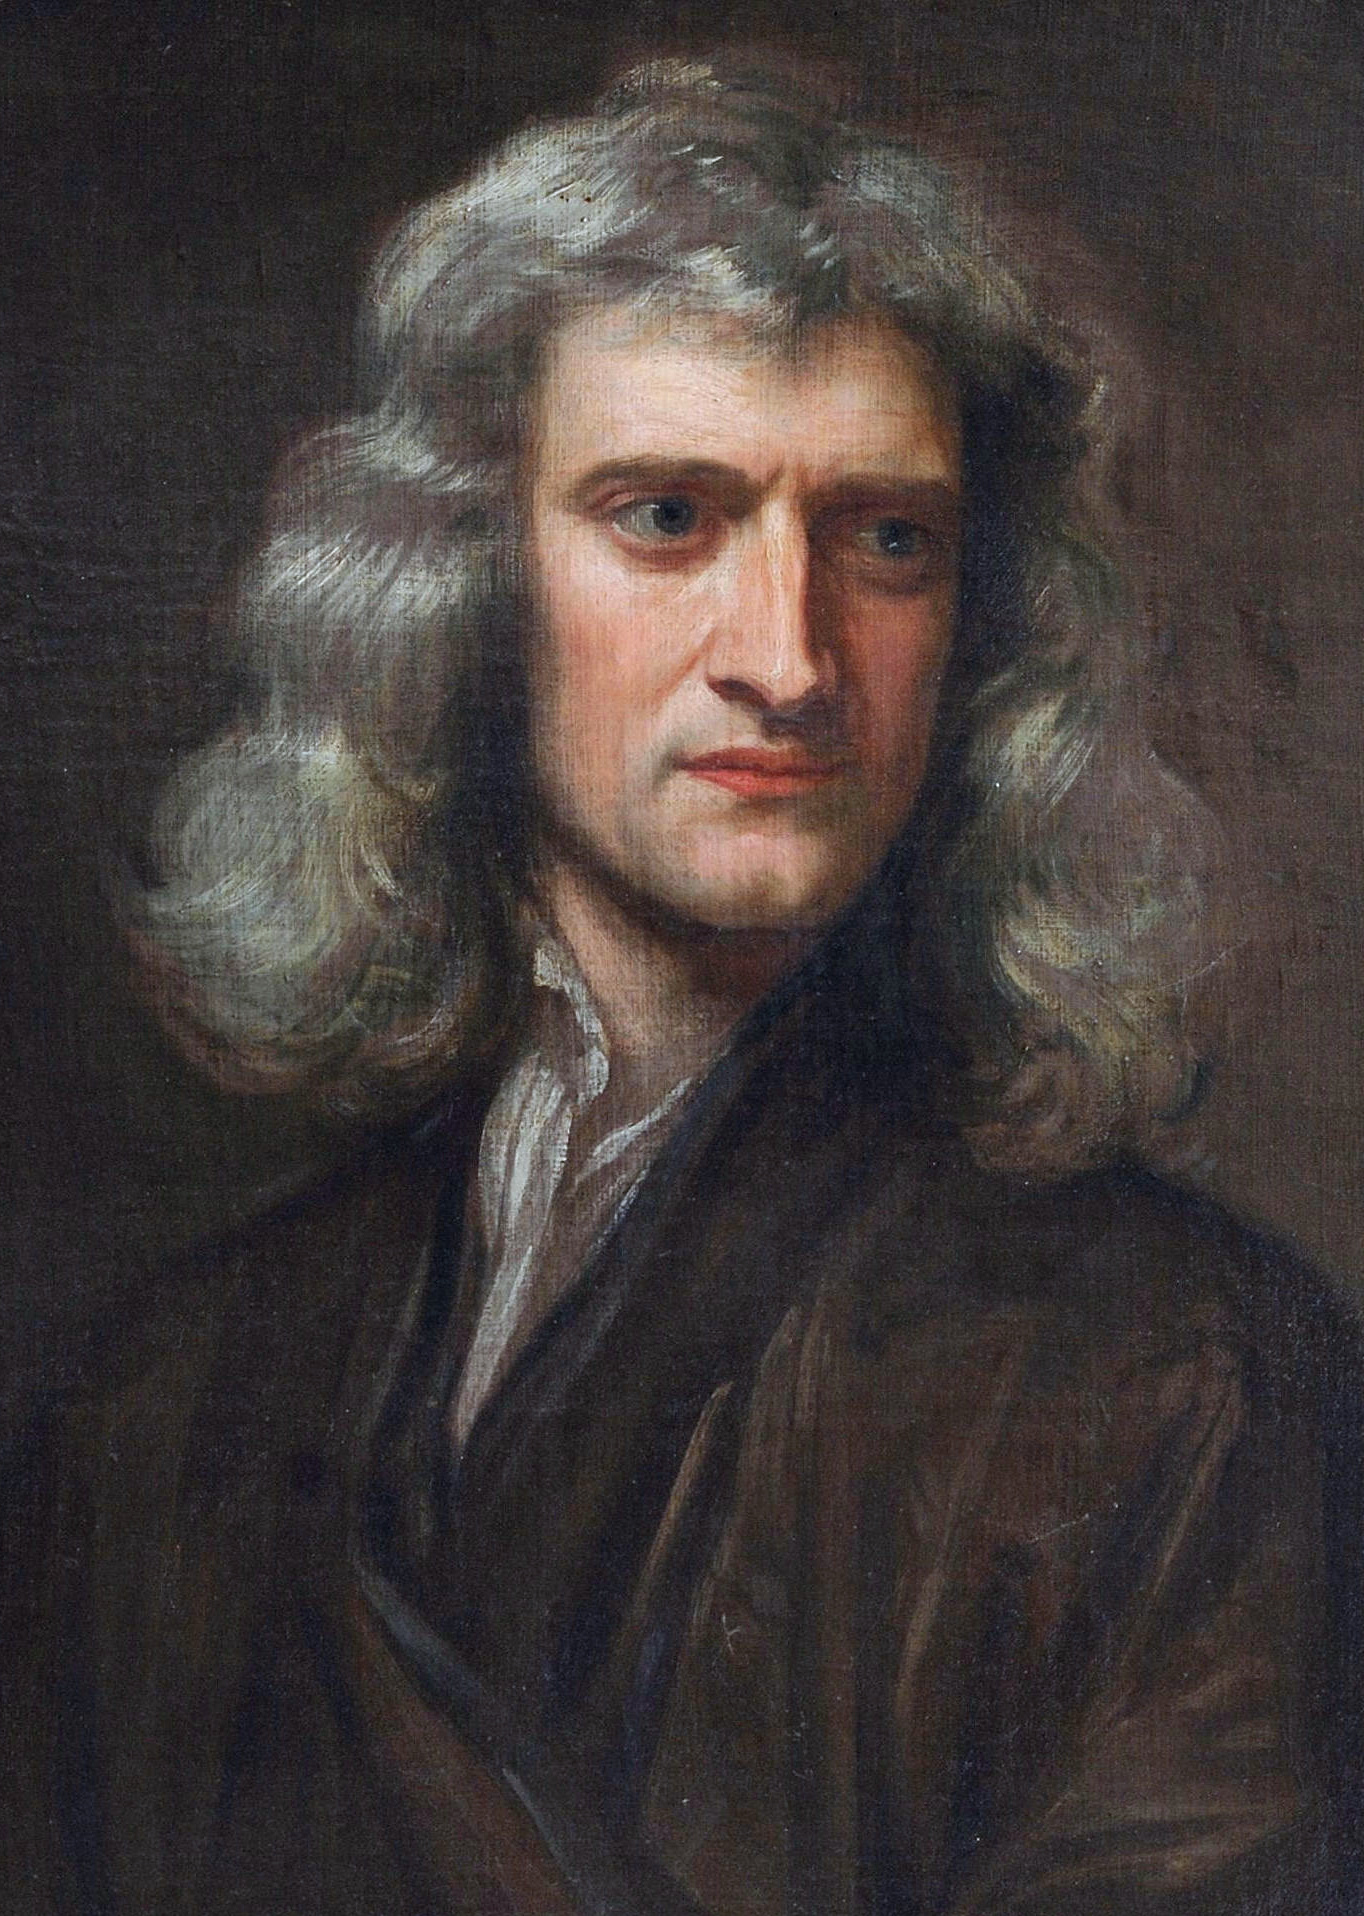
\includegraphics[width=0.92\textwidth]{images/newton.jpg}
\vspace{4pt}
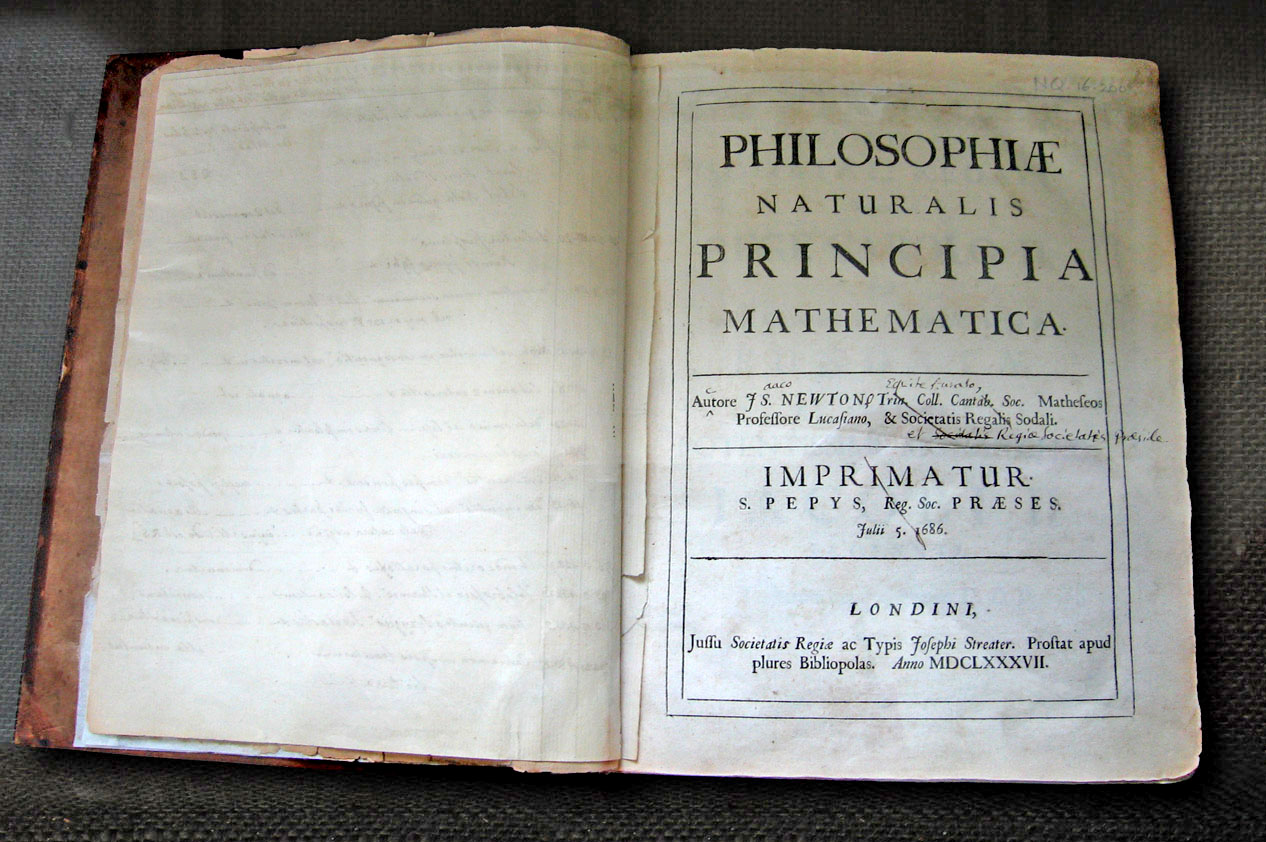
\includegraphics[width=0.92\textwidth]{images/principia.jpg}
\captionof{figure}{Isaac Newton (1642--1727) by Godfrey Kneller (1689), and the title page of \emph{Philosophiae Naturalis Principia Mathematica} (1687).}
\end{minipage}\hfill
\begin{minipage}{0.68\textwidth}
While isolated in Woolsthorpe Manor during the Great Plague of 1665--1666, Isaac Newton invented the calculus of fluxions, formulated the universal law of gravitation, and established the three laws of motion.

Encouraged and financed by astronomer Edmond Halley, Newton published his masterpiece \emph{Philosophiae Naturalis Principia Mathematica} in July 1687. The treatise unified terrestrial mechanics (falling apples, tides, pendulums) and celestial mechanics (Kepler's planetary ellipses) under a single mathematical framework, inaugurating the scientific revolution.
\end{minipage}
\end{historicalbox}

\begin{lawbox}{Newton's First Law (The Law of Inertia)}
There exist reference frames, called \textbf{inertial (or Galilean) reference frames}, in which any material point not subjected to external net forces (or subjected to forces whose vector sum is zero) preserves its state of rest or of uniform rectilinear motion:
\[
\sum\vec{F} = \vzero \implies \vec{v} = \text{constant vector.}
\]
\end{lawbox}

The First Law is not a mere special case of the Second Law: it asserts the \textbf{physical existence} of inertial reference frames, against which accelerations can be objectively measured.

\begin{definitionbox}{Linear Momentum}
The \textbf{linear momentum} $\vec{p}$ of a material point of inertial mass $m$ moving with velocity $\vec{v}$ is:
\[
\boxed{\vec{p} = m\,\vec{v}.}
\]
Momentum has dimensions $[\vec{p}] = \mathsf{M\,L\,T^{-1}}$ and is measured in $\mathrm{kg\,m\,s^{-1}} = \mathrm{N\,s}$.
\end{definitionbox}

\begin{lawbox}{Newton's Second Law (Fundamental Law of Dynamics)}
In an inertial reference frame, the net force $\sum\vec{F}$ acting on a material point is equal to the time rate of change of its linear momentum:
\[
\boxed{\sum\vec{F} = \frac{\dd\vec{p}}{\dd t}.}
\]
When the mass $m$ of the particle is constant ($m = \text{const}$):
\[
\boxed{\sum\vec{F} = m\frac{\dd\vec{v}}{\dd t} = m\,\vec{a}.}
\]
\end{lawbox}

\begin{lawbox}{Newton's Third Law (Law of Action and Reaction)}
Whenever body $1$ exerts a force $\vec{F}_{1\to 2}$ on body $2$, body $2$ simultaneously exerts an equal and opposite force $\vec{F}_{2\to 1}$ on body $1$:
\[
\boxed{\vec{F}_{2\to 1} = -\vec{F}_{1\to 2}.}
\]
Furthermore, for point particles interacting via central forces, both forces act along the common line connecting the two particles (\emph{strong form} of the third law).
\end{lawbox}

\begin{cautionbox}
\textbf{Action and reaction never cancel each other!} Because $\vec{F}_{1\to 2}$ acts exclusively on body $2$ while $\vec{F}_{2\to 1}$ acts exclusively on body $1$, they appear in separate Free-Body Diagrams. They cancel only when computing the total internal force on the combined system $(1 + 2)$.
\end{cautionbox}

\section{The Free-Body Diagram (FBD) Protocol}

To apply Newton's second law successfully, follow this rigorous algorithm:
\begin{enumerate}[leftmargin=1.6em,itemsep=3pt]
  \item \textbf{Isolate the body}: Mentally detach the chosen material point from all surrounding objects.
  \item \textbf{Inventory all external forces}:
        \begin{itemize}[leftmargin=1.2em]
          \item Field forces (acting at a distance): Gravity $\vec{P} = m\vec{g}$.
          \item Contact forces (from physical touch): Normal force $\vec{N}$ (perpendicular to surface), friction $\vec{f}$ (tangential), string tension $\vec{T}$ (pulling along string).
        \end{itemize}
  \item \textbf{Choose coordinate axes wisely}: Align one axis parallel to the expected direction of acceleration (or along the incline).
  \item \textbf{Project and solve}: Write $\sum F_x = m a_x$ and $\sum F_y = m a_y$.
\end{enumerate}

\begin{figure}[htbp]
\centering
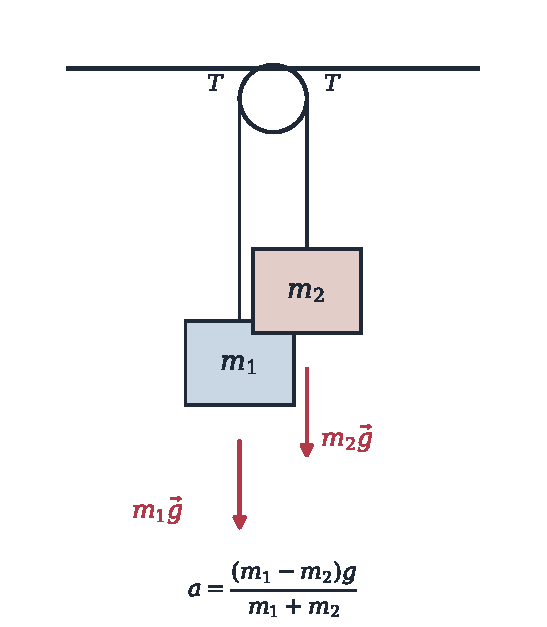
\includegraphics[width=0.65\textwidth]{figures/12_atwood.pdf}
\caption{The Atwood Machine. Two masses $m_1$ and $m_2$ suspended over an ideal frictionless pulley.}
\label{fig:atwood}
\end{figure}

\section{Extensive Worked Examples}

\begin{workedexample}{The Atwood Machine (Precision Measurement of $g$)}
In 1784, English mathematician George Atwood designed an apparatus to measure gravitational acceleration $g$ by diluting it using two connected masses $m_1$ and $m_2$ ($m_1 > m_2$) connected by an inextensible light cord passing over an ideal frictionless pulley.
(a) Draw the FBD for each mass and find the downward acceleration $a$ of mass $m_1$.
(b) Find the tension $T$ in the cord.
(c) For $m_1 = 1.050\ \mathrm{kg}$ and $m_2 = 1.000\ \mathrm{kg}$, compute $a$ and $T$.

\paragraph{Solution.}

(a) Let the downward direction be positive for $m_1$, and upward positive for $m_2$.
Because the cord is inextensible and taut, both masses have identical acceleration magnitude $a$:
\begin{itemize}[leftmargin=1.4em,itemsep=2pt]
  \item For $m_1$: Gravity pulls down ($+m_1 g$), tension pulls up ($-T$):
        \[
        m_1 g - T = m_1 a.
        \]
  \item For $m_2$: Tension pulls up ($+T$), gravity pulls down ($-m_2 g$):
        \[
        T - m_2 g = m_2 a.
        \]
\end{itemize}
Adding the two equations eliminates the unknown tension $T$:
\[
(m_1 g - T) + (T - m_2 g) = (m_1 + m_2)a \implies (m_1 - m_2)g = (m_1 + m_2)a.
\]
Solving for the acceleration:
\[
\boxed{a = \frac{m_1 - m_2}{m_1 + m_2}g.}
\]
Notice that by choosing $m_1 \approx m_2$, the acceleration $a$ can be made arbitrarily small, allowing precise timing with simple clocks!

(b) Substituting $a$ back into the $m_2$ equation:
\[
T = m_2(g + a) = m_2\left( g + \frac{m_1 - m_2}{m_1 + m_2}g \right) = m_2 g\left( \frac{m_1 + m_2 + m_1 - m_2}{m_1 + m_2} \right).
\]
Therefore:
\[
\boxed{T = \frac{2 m_1 m_2}{m_1 + m_2}g.}
\]
Notice that $T$ is the \textbf{harmonic mean} of the two weights: $T = 2\frac{P_1 P_2}{P_1 + P_2}$.

(c) Numerical evaluation:
Mass difference: $m_1 - m_2 = 1.050 - 1.000 = 0.050\ \mathrm{kg}$.
Total mass: $m_1 + m_2 = 1.050 + 1.000 = 2.050\ \mathrm{kg}$.
\[
a = \frac{0.050}{2.050}\times 9.81 = \frac{1}{41}\times 9.81 \approx \mathbf{0.239\ \mathrm{m\,s^{-2}}.}
\]
Tension:
\[
T = \frac{2(1.050)(1.000)}{2.050}\times 9.81 = \frac{2.100}{2.050}\times 9.81 \approx \mathbf{10.05\ \mathrm{N}.}
\]
The acceleration is diluted by a factor of 41 compared to free fall, making motion easily observable by human eyes.
\end{workedexample}

\begin{workedexample}{Connected Masses on a Smooth Double Incline}
Two masses $m_1$ and $m_2$ sit on a smooth triangular wedge with incline angles $\alpha$ and $\beta$. They are connected by a light cord passing over a smooth pulley at the apex.
(a) Find the condition for static equilibrium.
(b) Find the acceleration $a$ if the system is released from rest.
(c) Find the tension $T$ in the cord during motion.

\paragraph{Solution.}

(a) Set the coordinate $s$ along the string, positive in the direction where $m_1$ slides down its incline and $m_2$ slides up its incline:
\begin{itemize}[leftmargin=1.4em,itemsep=2pt]
  \item Along incline 1: $m_1 g\sin\alpha - T = m_1 a$.
  \item Along incline 2: $T - m_2 g\sin\beta = m_2 a$.
\end{itemize}
For static equilibrium ($a = 0$):
\[
T = m_1 g\sin\alpha = m_2 g\sin\beta \implies \boxed{m_1\sin\alpha = m_2\sin\beta.}
\]
This iconic equilibrium condition was discovered by Flemish engineer Simon Stevin in 1586 using his famous \emph{clootcrans} (wreath of spheres) thought experiment!

(b) Adding the two equations of motion:
\[
m_1 g\sin\alpha - m_2 g\sin\beta = (m_1 + m_2)a \implies \boxed{a = g\frac{m_1\sin\alpha - m_2\sin\beta}{m_1 + m_2}.}
\]
If $m_1\sin\alpha > m_2\sin\beta$, $m_1$ accelerates down incline 1; if $m_1\sin\alpha < m_2\sin\beta$, $m_2$ accelerates down incline 2.

(c) Tension during motion:
\[
T = m_2 g\sin\beta + m_2 a = m_2 g\sin\beta + m_2 g\frac{m_1\sin\alpha - m_2\sin\beta}{m_1 + m_2}.
\]
Bringing to a common denominator:
\[
T = \frac{m_2 g(m_1\sin\beta + m_2\sin\beta + m_1\sin\alpha - m_2\sin\beta)}{m_1 + m_2} = \boxed{\frac{m_1 m_2 g(\sin\alpha + \sin\beta)}{m_1 + m_2}.}
\]
\end{workedexample}

\begin{workedexample}{Tension Distribution along a Heavy Accelerating Rope}
A heavy vertical rope of uniform linear density $\lambda = M/L$ and length $L$ is pulled vertically upward by a force $F_0$ applied at its top end ($y = L$).
(a) Find the upward acceleration $a$ of the rope.
(b) Determine the internal tension $T(y)$ at a distance $y \in [0, L]$ from the bottom free end.
(c) Where is the rope most likely to snap?

\paragraph{Solution.}

(a) The entire rope has mass $M$ and total weight $P = Mg$.
Applying Newton's second law to the rope as a single body:
\[
F_0 - Mg = Ma \implies \boxed{a = \frac{F_0}{M} - g.}
\]
For upward acceleration, $F_0 > Mg$.

(b) To find the internal tension $T(y)$ at height $y$, make a cross-sectional cut at height $y$ and isolate the lower segment from $0$ to $y$:
\begin{itemize}[leftmargin=1.4em,itemsep=2pt]
  \item Mass of the lower segment: $m(y) = \lambda y = M\frac{y}{L}$.
  \item Weight of the lower segment: $P(y) = m(y)g = \lambda y g$.
  \item Upward force acting on the cut face from the upper segment: tension $T(y)$.
  \item Acceleration of the lower segment: $a = \frac{F_0}{M} - g$ (same as the whole rope).
\end{itemize}
Applying Newton's second law to the lower segment:
\[
T(y) - m(y)g = m(y)a \implies T(y) = m(y)(g + a).
\]
Substitute $g + a = \frac{F_0}{M}$:
\[
T(y) = \left(M\frac{y}{L}\right)\left(\frac{F_0}{M}\right) = \boxed{F_0\frac{y}{L}.}
\]
The tension varies \textbf{linearly} from $0$ at the bottom free end to $F_0$ at the top:
\begin{itemize}[leftmargin=1.4em,itemsep=2pt]
  \item At the bottom free end ($y = 0$): $T(0) = 0$ (no mass suspended below).
  \item At the midpoint ($y = L/2$): $T(L/2) = \frac{1}{2}F_0$.
  \item At the top support ($y = L$): $T(L) = F_0$.
\end{itemize}

(c) Because tension is maximum at the very top ($y = L$), any heavy accelerating rope, cable, or elevator hoist line is \textbf{always most vulnerable to snapping at its uppermost attachment point}.
\end{workedexample}

\chapter{Contact Forces, Solid Friction, and Mechanical Constraints}
\label{ch:friction_constraints}

\begin{chapterintro}
\textbf{Chapter Objectives:} Contact forces transmit the interactions that prevent matter from interpenetrating. In this chapter, you will master the Amontons-Coulomb laws of dry friction; construct the friction cone; derive the exponential Capstan formula for ropes wound around cylinders; analyze banked turns; and solve multi-tier stacked body problems with static and kinetic thresholds.
\end{chapterintro}

\section{The Nature of Contact Forces}

When two physical bodies touch, the microscopic electrostatic repulsion between electron clouds in their outer atomic layers prevents interpenetration. At the macroscopic scale, this distributed contact stress is resolved into two orthogonal components:
\[
\boxed{\vec{R} = \vec{N} + \vec{f},}
\]
where:
\begin{itemize}[leftmargin=1.4em,itemsep=3pt]
  \item $\vec{N}$ is the \textbf{Normal Force}, perpendicular to the contact tangent plane, preventing interpenetration ($N \ge 0$).
  \item $\vec{f}$ is the \textbf{Frictional Force}, parallel to the contact tangent plane, opposing relative sliding.
\end{itemize}

\begin{figure}[htbp]
\centering
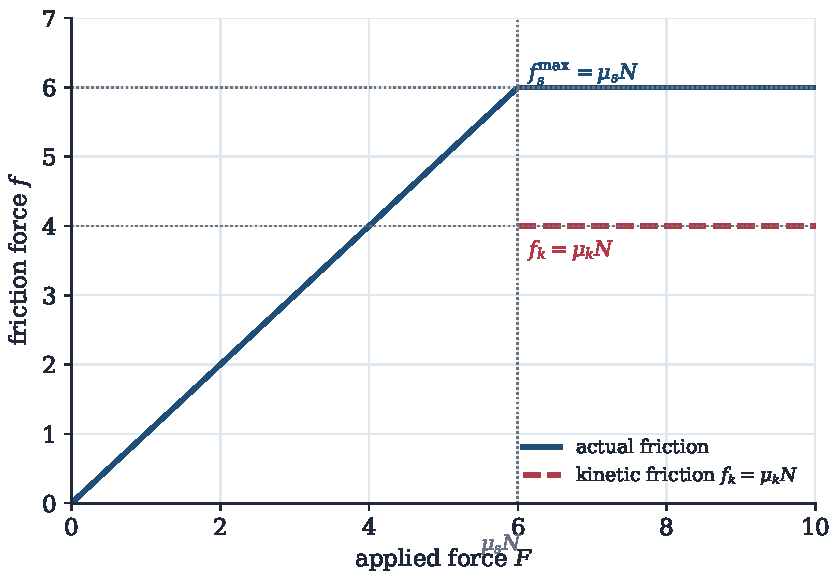
\includegraphics[width=0.74\textwidth]{figures/13_friction.pdf}
\caption{The classic friction response curve. As tangential force $F$ increases, static friction matches it identically until the peak $\mu_s N$. Once sliding begins, kinetic friction drops to the constant level $\mu_k N$.}
\label{fig:friction_curve}
\end{figure}

\section{The Amontons-Coulomb Laws of Dry Friction}

Formulated experimentally by Guillaume Amontons (1699) and refined by Charles-Augustin de Coulomb (1781):
\begin{lawbox}{Coulomb's Laws of Solid Friction}
\begin{enumerate}[leftmargin=1.5em,itemsep=3pt]
  \item \textbf{Static Friction ($v_{\text{rel}} = 0$)}: Prevents the initiation of sliding. It acts as an adjustable constraint force matching the applied tangential load up to a sharp threshold:
        \[
        \boxed{f_s \le \mu_s\,N,}
        \]
        where $\mu_s$ is the dimensionless \textbf{coefficient of static friction}.
  \item \textbf{Kinetic Friction ($v_{\text{rel}} \ne 0$)}: Resists established sliding motion, oriented strictly opposite to the relative velocity:
        \[
        \boxed{\vec{f}_k = -\mu_k\,N\,\frac{\vec{v}_{\text{rel}}}{\norm{\vec{v}_{\text{rel}}}},}
        \]
        where $\mu_k$ is the \textbf{coefficient of kinetic friction}. In virtually all physical material pairings, $\mu_k < \mu_s$.
  \item \textbf{Area Independence}: To a remarkable approximation, $f$ is independent of the apparent geometric contact area between the surfaces.
\end{enumerate}
\end{lawbox}

\begin{figure}[htbp]
\centering
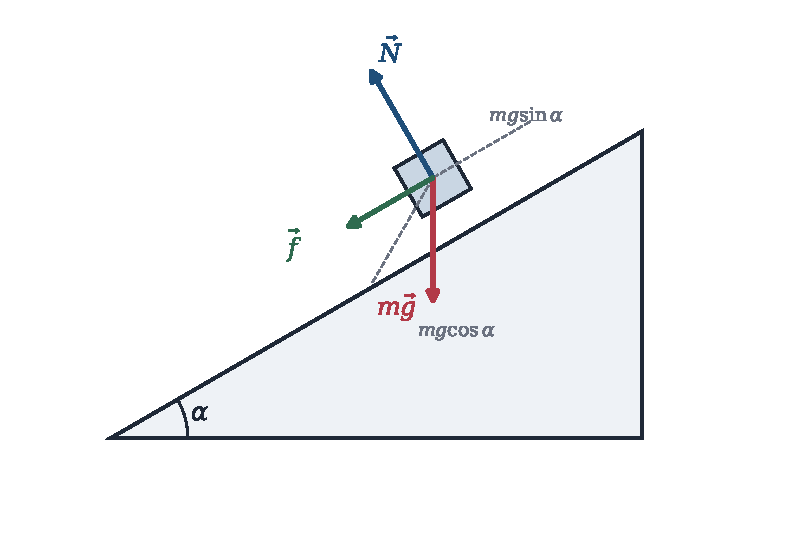
\includegraphics[width=0.74\textwidth]{figures/11_incline_fbd.pdf}
\caption{Free-Body Diagram of a block on a rough incline of angle $\alpha$. Normal force $N = mg\cos\alpha$ and friction $f$ oppose gravity's downhill pull $mg\sin\alpha$.}
\label{fig:incline_fbd}
\end{figure}

\begin{definitionbox}{The Friction Cone and Angle of Repose}
The total contact reaction vector $\vec{R} = \vec{N} + \vec{f}$ makes an angle $\phi$ with the normal:
\[
\tan\phi = \frac{f}{N}.
\]
At the threshold of impending motion ($f = \mu_s N$), the angle reaches its maximum value $\phi_s$:
\[
\boxed{\tan\phi_s = \mu_s.}
\]
The cone of half-angle $\phi_s$ around the normal is the \textbf{Friction Cone}. If the resultant applied external load falls inside this cone, sliding is physically impossible regardless of how large the force is!
The \textbf{angle of repose} $\alpha_c$ of an incline is precisely $\alpha_c = \phi_s = \arctan\mu_s$.
\end{definitionbox}

\section{Extensive Worked Examples}

\begin{workedexample}{Minimum Force to Pull a Crate on a Rough Floor}
A heavy crate of mass $m$ rests on a rough horizontal floor with static friction coefficient $\mu_s$. A rope pulls the crate with force $\vec{F}$ inclined at angle $\theta$ above the horizontal.
(a) Find the magnitude of force $F(\theta)$ required to initiate motion.
(b) Find the optimal pulling angle $\theta_{\text{opt}}$ that minimizes the required pulling force $F$, and calculate $F_{\min}$.

\paragraph{Solution.}

(a) Set up horizontal and vertical axes:
\begin{align*}
\text{Vertical balance:}\quad & N + F\sin\theta - mg = 0 \implies N = mg - F\sin\theta, \\
\text{Horizontal balance:}\quad & F\cos\theta - f_s = 0 \implies f_s = F\cos\theta.
\end{align*}
Sliding begins when static friction reaches its maximum threshold $f_s = \mu_s N$:
\[
F\cos\theta = \mu_s(mg - F\sin\theta) = \mu_s mg - \mu_s F\sin\theta.
\]
Rearranging terms:
\[
F(\cos\theta + \mu_s\sin\theta) = \mu_s mg \implies \boxed{F(\theta) = \frac{\mu_s mg}{\cos\theta + \mu_s\sin\theta}.}
\]

(b) To minimize $F(\theta)$, we maximize the denominator $D(\theta) = \cos\theta + \mu_s\sin\theta$.
Differentiating with respect to $\theta$:
\[
D'(\theta) = -\sin\theta + \mu_s\cos\theta = 0 \implies \boxed{\tan\theta_{\text{opt}} = \mu_s.}
\]
The optimal pulling angle is precisely equal to the \textbf{angle of friction} $\phi_s$!
At this optimal angle:
\[
\cos\theta_{\text{opt}} = \frac{1}{\sqrt{1 + \mu_s^2}}, \qquad \sin\theta_{\text{opt}} = \frac{\mu_s}{\sqrt{1 + \mu_s^2}}.
\]
The maximum denominator value is:
\[
D(\theta_{\text{opt}}) = \frac{1}{\sqrt{1 + \mu_s^2}} + \frac{\mu_s^2}{\sqrt{1 + \mu_s^2}} = \frac{1 + \mu_s^2}{\sqrt{1 + \mu_s^2}} = \sqrt{1 + \mu_s^2}.
\]
Therefore, the absolute minimum force required is:
\[
\boxed{F_{\min} = \frac{\mu_s mg}{\sqrt{1 + \mu_s^2}} = mg\sin\phi_s.}
\]
Pulling slightly upward reduces the normal force $N$, which dramatically reduces friction, requiring much less effort than pulling horizontally ($F(0) = \mu_s mg$).
\end{workedexample}

\begin{workedexample}{The Capstan Equation (Belt Friction)}
A flexible rope is wrapped around a fixed rough horizontal cylinder of circular cross-section with coefficient of friction $\mu$. The rope subtends a total contact wrap angle $\theta$ (in radians).
A tension $T_1$ is applied to one end.
Prove the celebrated \textbf{Eytelwein--Capstan Formula} for the maximum holding tension $T_2$ at the other end before slipping:
\[
T_2 = T_1\,e^{\mu\theta}.
\]

\paragraph{Solution.}

Isolate an infinitesimal segment of the rope subtending an angle $\dd\theta$:
\begin{itemize}[leftmargin=1.4em,itemsep=2pt]
  \item Tension at angle $\theta$: $T$.
  \item Tension at angle $\theta + \dd\theta$: $T + \dd T$.
  \item Normal reaction from the cylinder: $\dd N$ directed radially outward.
  \item Maximum static friction force: $\dd f = \mu\,\dd N$ directed along the tangent opposing slipping.
\end{itemize}
Projecting forces along the radial and tangential directions:
\begin{align*}
\text{Radial:}\quad & \dd N - (T + \dd T)\sin\left(\frac{\dd\theta}{2}\right) - T\sin\left(\frac{\dd\theta}{2}\right) = 0.
\end{align*}
For infinitesimal angles, $\sin(\dd\theta/2) \approx \dd\theta/2$:
\[
\dd N = 2T\frac{\dd\theta}{2} + \dd T\frac{\dd\theta}{2} \approx T\,\dd\theta.
\]
(The second-order term $\dd T\dd\theta$ is discarded).

Projecting along the tangential direction:
\begin{align*}
\text{Tangential:}\quad & (T + \dd T)\cos\left(\frac{\dd\theta}{2}\right) - T\cos\left(\frac{\dd\theta}{2}\right) - \dd f = 0.
\end{align*}
With $\cos(\dd\theta/2) \approx 1$ and $\dd f = \mu\,\dd N$:
\[
\dd T = \dd f = \mu\,\dd N.
\]
Substitute $\dd N = T\,\dd\theta$:
\[
\dd T = \mu\,T\,\dd\theta \implies \frac{\dd T}{T} = \mu\,\dd\theta.
\]
Integrating across the entire wrap angle from $\theta = 0$ (tension $T_1$) to angle $\theta$ (tension $T_2$):
\[
\int_{T_1}^{T_2} \frac{\dd T}{T} = \mu\int_0^\theta \dd\theta' \implies \ln\left(\frac{T_2}{T_1}\right) = \mu\theta.
\]
Exponentiating both sides yields the famous \textbf{Capstan Equation}:
\[
\boxed{T_2 = T_1\,e^{\mu\theta}.}
\]
\textbf{Remarkable Physical Consequence:}
Because of the exponential dependence, friction grows extraordinarily fast with the number of turns $n$ ($\theta = 2\pi n$).
For a rope on an iron bollard with $\mu = 0.40$ wrapped $3$ full turns ($n = 3 \implies \theta = 6\pi \approx 18.85\ \mathrm{rad}$):
\[
\frac{T_2}{T_1} = e^{0.40\times 18.85} = e^{7.54} \approx \mathbf{1882.}
\]
A single sailor holding the line with a gentle force of $T_1 = 50\ \mathrm{N}$ (about $5\ \mathrm{kg}$ of pull) can hold a massive ship exerting $T_2 = 1882\times 50 \approx \mathbf{94\,100\ \mathrm{N}}$ (equivalent to nearly $10$ metric tons)!
\end{workedexample}

\begin{workedexample}{Maximum Cornering Speed on a Banked Highway}
A civil engineer designs a highway curve of radius $R = 200\ \mathrm{m}$ banked at an angle $\theta = 15.0^\circ$. The coefficient of static friction between car tires and the road surface is $\mu_s = 0.500$.
(a) Find the \textbf{rated speed} $v_0$ for which no friction is needed to negotiate the turn safely.
(b) Find the maximum speed $v_{\max}$ before the car slips up the bank.
(c) Find the minimum speed $v_{\min}$ below which the car slides down the bank.

\paragraph{Solution.}

(a) Rated speed ($f = 0$):
Gravity pulls down ($-mg$), and the normal force $\vec{N}$ provides both vertical support and horizontal centripetal acceleration:
\begin{align*}
N\cos\theta &= mg, \\
N\sin\theta &= m\frac{v_0^2}{R}.
\end{align*}
Dividing gives $\tan\theta = \frac{v_0^2}{gR}$:
\[
\boxed{v_0 = \sqrt{gR\tan\theta}.}
\]
Computing:
\[
v_0 = \sqrt{(9.81)(200)\tan 15.0^\circ} = \sqrt{1962\times 0.2679} = \sqrt{525.7} \approx \mathbf{22.9\ \mathrm{m\,s^{-1}}} \approx 82.5\ \mathrm{km\,h^{-1}}.
\]

(b) Maximum speed $v_{\max}$ (impending slip up the bank):
Friction points down the incline: $f_s = \mu_s N$.
Equations of motion:
\begin{align*}
\text{Vertical:}\quad & N\cos\theta - \mu_s N\sin\theta = mg \implies N(\cos\theta - \mu_s\sin\theta) = mg, \\
\text{Horizontal:}\quad & N\sin\theta + \mu_s N\cos\theta = m\frac{v_{\max}^2}{R} \implies N(\sin\theta + \mu_s\cos\theta) = m\frac{v_{\max}^2}{R}.
\end{align*}
Dividing the two equations:
\[
\frac{v_{\max}^2}{gR} = \frac{\sin\theta + \mu_s\cos\theta}{\cos\theta - \mu_s\sin\theta} = \frac{\tan\theta + \mu_s}{1 - \mu_s\tan\theta}.
\]
Solving for $v_{\max}$:
\[
\boxed{v_{\max} = \sqrt{gR\left( \frac{\tan\theta + \mu_s}{1 - \mu_s\tan\theta} \right)}.}
\]
Numerical calculation:
\[
\frac{0.2679 + 0.500}{1 - (0.500)(0.2679)} = \frac{0.7679}{1 - 0.1340} = \frac{0.7679}{0.8660} \approx 0.8867.
\]
\[
v_{\max} = \sqrt{1962\times 0.8867} = \sqrt{1739.7} \approx \mathbf{41.7\ \mathrm{m\,s^{-1}}} \approx \mathbf{150\ \mathrm{km\,h^{-1}}.}
\]

(c) Minimum speed $v_{\min}$ (impending slip down the bank):
Friction points up the incline: $\mu_s \to -\mu_s$:
\[
\boxed{v_{\min} = \sqrt{gR\left( \frac{\tan\theta - \mu_s}{1 + \mu_s\tan\theta} \right)}.}
\]
Since $\mu_s = 0.500 > \tan 15^\circ = 0.268$, static friction can hold the car even at rest ($v = 0$); hence $\mathbf{v_{\min} = 0\ \mathrm{m\,s^{-1}}}$.
The car will not slide down even if stopped in an icy traffic jam.
\end{workedexample}

\chapter{Dynamics in Non-Inertial Reference Frames}
\label{ch:noninertial_text}

\begin{chapterintro}
\textbf{Chapter Objectives:} When studying phenomena on the rotating Earth or in accelerating vehicles, we observe from non-inertial frames. In this chapter, you will master the fundamental equation of relative dynamics; calculate centrifugal and Coriolis fictitious forces; understand plumb line deflections and the flattening of the Earth; explain why cyclones spin counter-clockwise in the Northern hemisphere; and solve the precession of the Foucault pendulum.
\end{chapterintro}

\section{The Equation of Relative Dynamics}

In an inertial frame $\mathcal{R}$, Newton's second law is strictly valid: $m\vec{a}_a = \sum\vec{F}_{\text{real}}$.
Substituting the kinematic composition of accelerations $\vec{a}_a = \vec{a}_r + \vec{a}_e + \vec{a}_c$:
\[
m\left(\vec{a}_r + \vec{a}_e + \vec{a}_c\right) = \sum\vec{F}_{\text{real}}.
\]
Rearranging to isolate the relative acceleration $\vec{a}_r$ as seen by the moving observer:
\[
\boxed{m\vec{a}_r = \sum\vec{F}_{\text{real}} + \vec{F}_{ie} + \vec{F}_{ic}}
\]
where the two \textbf{fictitious (inertial) forces} are:
\begin{align}
\vec{F}_{ie} &= -m\vec{a}_e \quad \text{(\textbf{Inertial Force of Transport / Centrifugal Force})}, \\
\vec{F}_{ic} &= -m\vec{a}_c = -2m\,\vec{\Omega}\times\vec{v}_r \quad \text{(\textbf{Coriolis Force})}.
\end{align}

\begin{historicalbox}{Léon Foucault and the Panthéon Demonstration (1851)}
\begin{minipage}{0.30\textwidth}
\centering
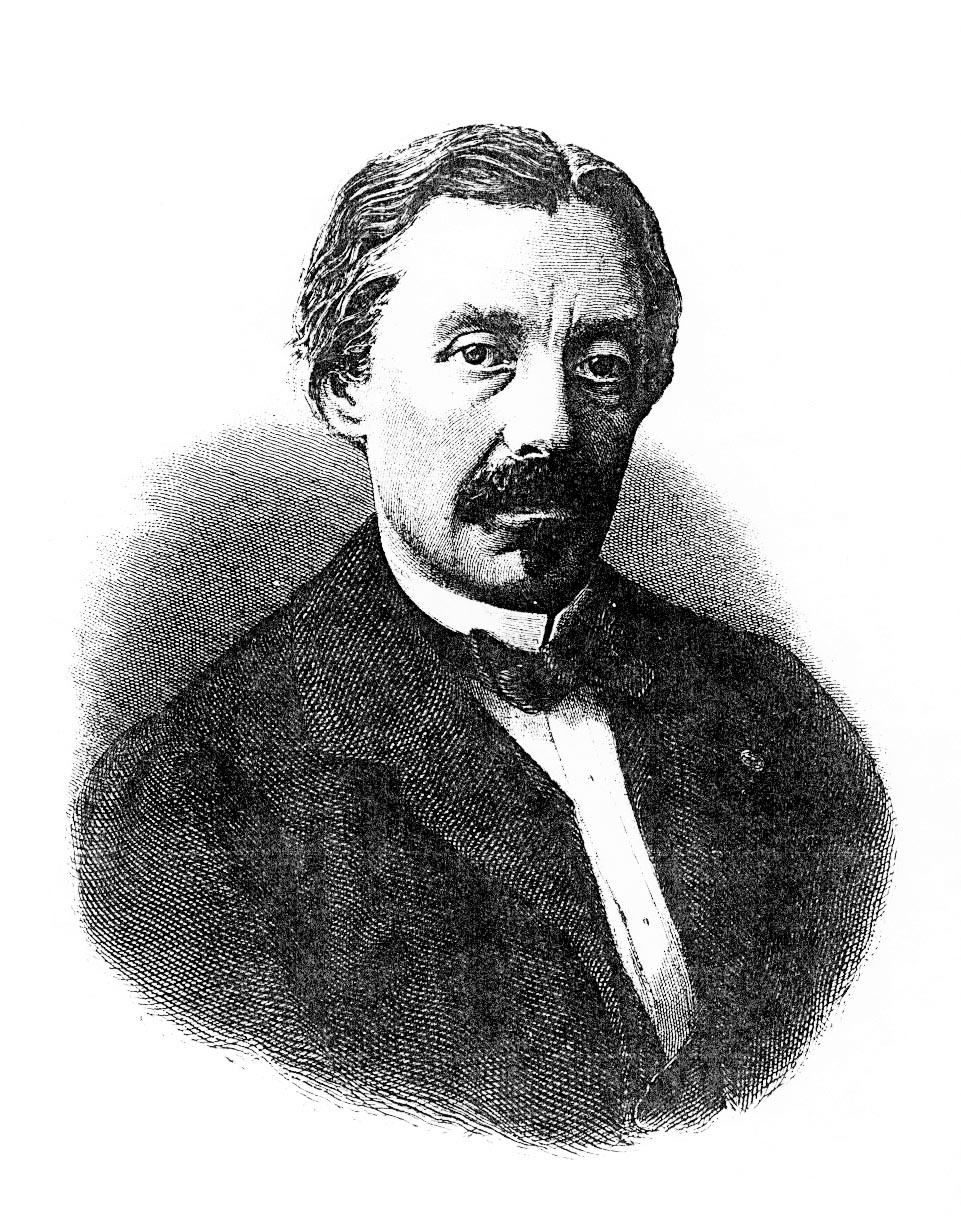
\includegraphics[width=0.92\textwidth]{images/foucault.jpg}
\vspace{4pt}
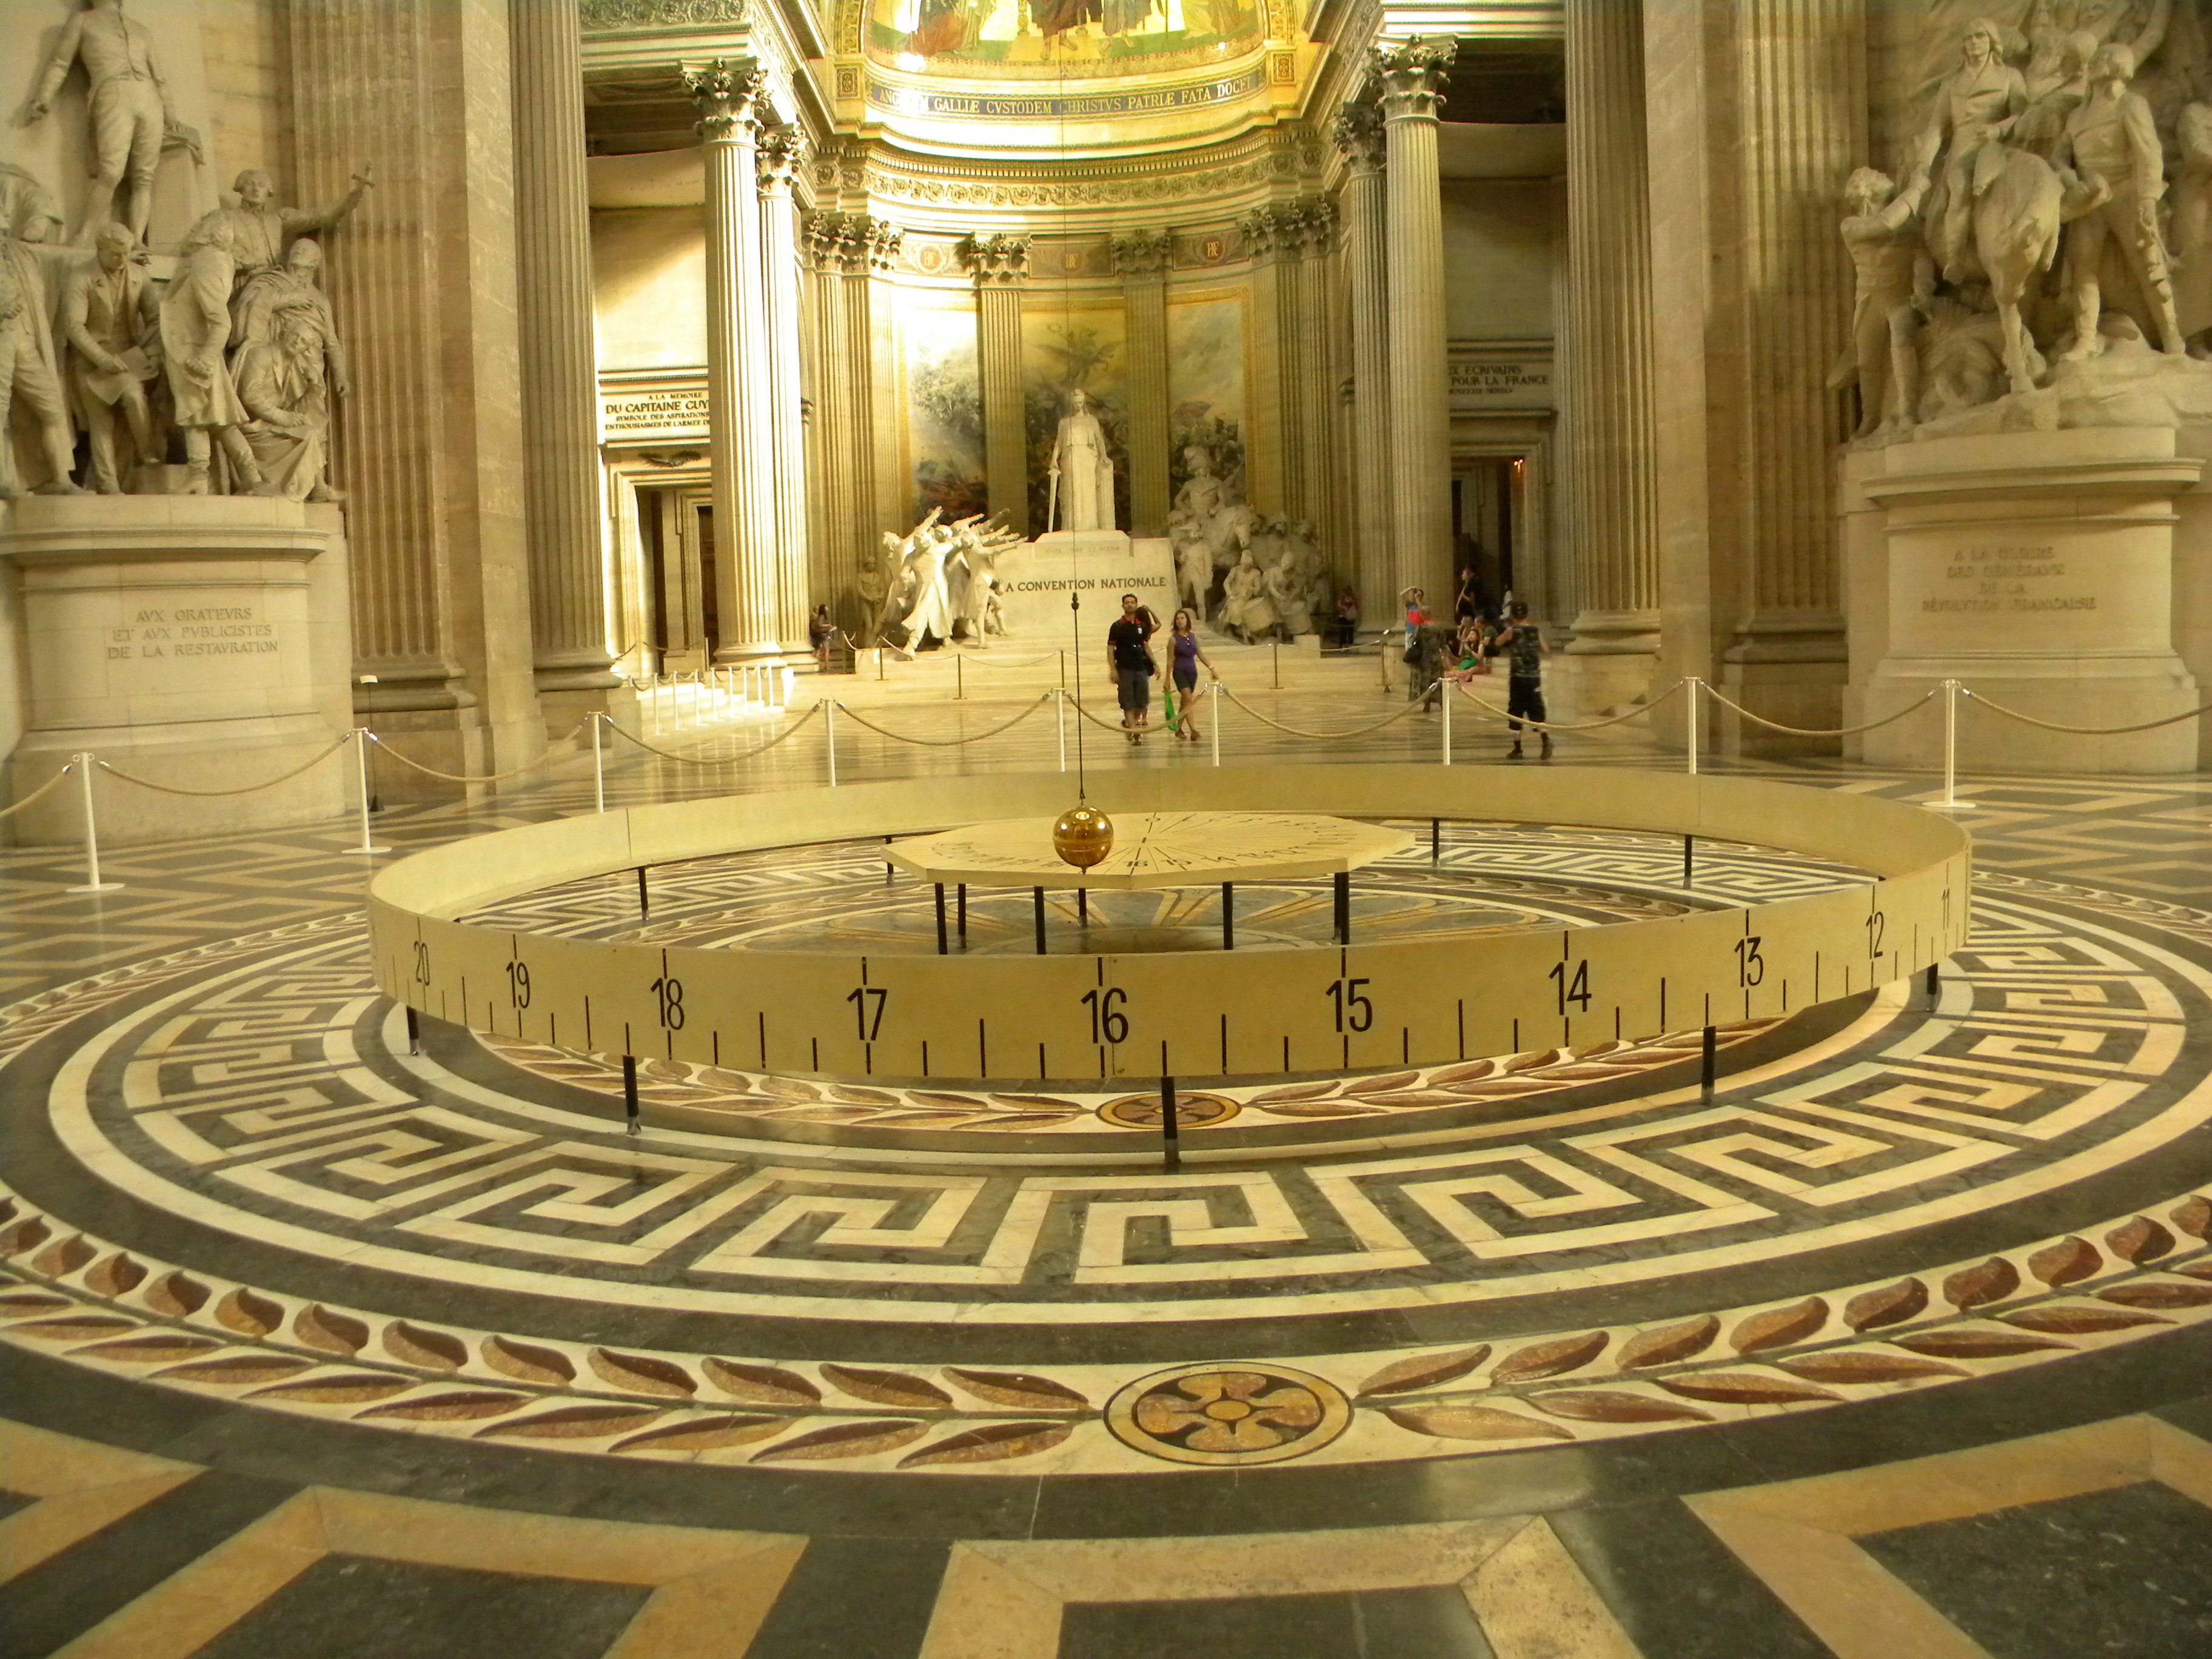
\includegraphics[width=0.92\textwidth]{images/foucault_pendulum.jpg}
\captionof{figure}{Léon Foucault (1819--1868), and the Foucault Pendulum suspended beneath the dome of the Panthéon in Paris.}
\end{minipage}\hfill
\begin{minipage}{0.66\textwidth}
In January 1851, French physicist Léon Foucault suspended a $28\ \mathrm{kg}$ brass-coated lead sphere from a $67\ \mathrm{m}$ steel wire inside the dome of the Panthéon in Paris. A spike on the bob traced lines in sand spread on the floor.

Before a mesmerized crowd, the plane of swing visibly rotated clockwise at roughly $11^\circ$ per hour, taking $31.8$ hours for a complete revolution. Foucault had devised the first purely dynamic, laboratory-based proof of Earth's rotation that did not require celestial observations: ``You are invited to see the Earth turn.''
\end{minipage}
\end{historicalbox}

\section{Centrifugal Force and Apparent Terrestrial Weight}

On the rotating Earth ($\vec{\Omega} = \Omega\khat$ with $\Omega \approx 7.292\times 10^{-5}\ \mathrm{rad\,s^{-1}}$), a body at rest relative to the surface ($\vec{v}_r = \vzero$) experiences zero Coriolis force.
However, it experiences the outward \textbf{centrifugal force}:
\[
\vec{F}_{\text{cf}} = -m\vec{\Omega}\times(\vec{\Omega}\times\vec{r}) = m\Omega^2 r_\perp\,\ur = m\Omega^2 R_E\cos\lambda\,\ur,
\]
where $\lambda$ is latitude and $r_\perp = R_E\cos\lambda$ is the distance to the polar axis.
The measured \textbf{apparent weight} is the resultant of true gravitational attraction and the centrifugal force:
\[
\boxed{\vec{P}_{\text{app}} = m\vec{g}_{\text{eff}} = m\vec{g}_0 + \vec{F}_{\text{cf}}.}
\]
\begin{itemize}[leftmargin=1.4em,itemsep=2pt]
  \item At the poles ($\lambda = \pm 90^\circ$): $r_\perp = 0 \implies \vec{F}_{\text{cf}} = \vzero$. Apparent gravity equals true gravity ($g_{\text{eff}} \approx 9.832\ \mathrm{m\,s^{-2}}$).
  \item At the equator ($\lambda = 0^\circ$): $\vec{F}_{\text{cf}}$ points directly opposite to gravity, reducing apparent weight by $\Omega^2 R_E \approx 0.034\ \mathrm{m\,s^{-2}}$ ($g_{\text{eff}} \approx 9.780\ \mathrm{m\,s^{-2}}$).
  \item At intermediate latitudes: $\vec{g}_{\text{eff}}$ is tilted slightly toward the equator, deflecting a hanging plumb line by up to $\theta \approx 6\ \text{arcminutes}$ from the true geometric center of Earth.
\end{itemize}

\section{Meteorological Consequences of the Coriolis Force}

\begin{figure}[htbp]
\centering
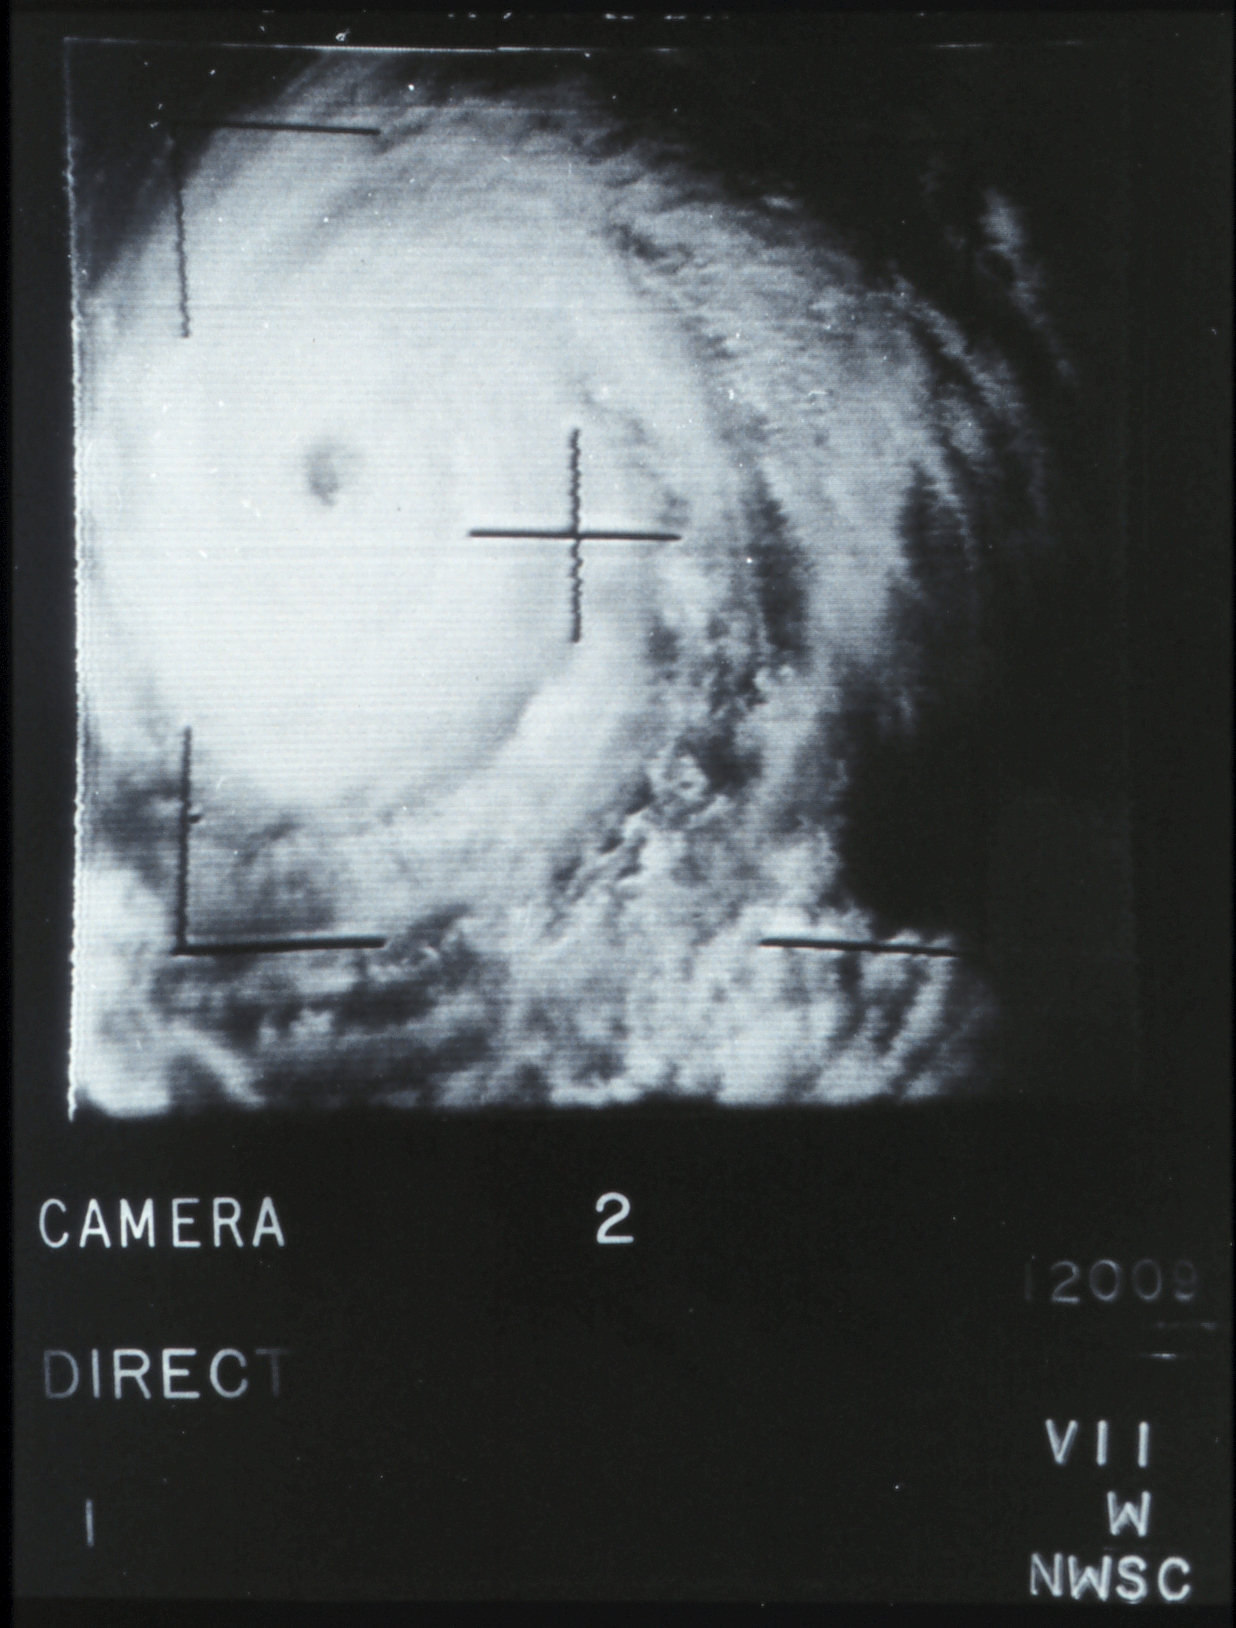
\includegraphics[width=0.62\textwidth]{images/cyclone_coriolis.jpg}
\caption{Early satellite photograph of a tropical cyclone displaying the classic counter-clockwise spiral in the Northern Hemisphere induced by the Coriolis deflection of inward-flowing air masses.}
\label{fig:cyclone}
\end{figure}

In the Northern hemisphere, Earth's angular velocity vector has an upward vertical component $\Omega_z = \Omega\sin\lambda > 0$.
The horizontal Coriolis force acting on horizontal air velocity $\vec{v}_r$ is:
\[
\vec{F}_{\text{Cor, horiz}} = -2m(\Omega\sin\lambda\khat)\times\vec{v}_r = 2m\Omega\sin\lambda(\vec{v}_r\times\khat).
\]
\begin{lawbox}{Buys Ballot's Law of Meteorology}
In the Northern hemisphere, the Coriolis force deflects every moving body \textbf{to its right}; in the Southern hemisphere, it deflects every moving body \textbf{to its left}.
When air rushes inward toward a low-pressure center (cyclone), this rightward deflection causes the inward streams to circulate \textbf{counter-clockwise} in the North, forming hurricanes and typhoons.
\end{lawbox}

\section{Extensive Worked Examples}

\begin{workedexample}{The Parabolic Liquid Telescope Mirror}
A cylindrical container filled with a reflective liquid (such as liquid mercury or molten gallium alloy) rotates about its central vertical axis at constant angular velocity $\omega$.
(a) In the rotating frame of the liquid, set up cylindrical coordinates $(r, \theta, z)$ and show that the effective gravity is $\vec{g}_{\text{eff}} = \omega^2 r\ur - g\khat$.
(b) Derive the equation of the free surface $z(r) = z_0 + \frac{\omega^2 r^2}{2g}$.
(c) Show that this surface forms a perfect parabolic mirror with focal length $f = \frac{g}{2\omega^2}$.
(d) For an astronomical telescope with focal length $f = 6.00\ \mathrm{m}$, compute the required rotation rate $\omega$ and rotational period in rpm.

\paragraph{Solution.}

(a) In the rotating frame $\mathcal{R}'$, the fluid is at rest ($\vec{v}_r = \vzero$, $\vec{F}_{\text{Cor}} = \vzero$).
The forces acting on a fluid element of mass $\dd m = \rho\,\dd V$ are:
\begin{itemize}[leftmargin=1.4em,itemsep=2pt]
  \item True gravity: $\dd\vec{P} = -(\dd m)g\khat$.
  \item Centrifugal force: $\dd\vec{F}_{\text{cf}} = +(\dd m)\omega^2 r\,\ur$.
\end{itemize}
The effective acceleration of gravity in $\mathcal{R}'$ is:
\[
\boxed{\vec{g}_{\text{eff}} = \frac{\dd\vec{P} + \dd\vec{F}_{\text{cf}}}{\dd m} = \omega^2 r\,\ur - g\khat.}
\]

(b) At hydrostatic equilibrium in $\mathcal{R}'$, the fluid pressure gradient satisfies $\vec{\nabla} p = \rho\vec{g}_{\text{eff}}$.
Along the free surface open to the atmosphere, $p \equiv p_{\text{atm}} = \text{const}$, so $\dd p = \vec{\nabla} p\cdot\dd\vec{r} = 0$:
\[
\rho\vec{g}_{\text{eff}}\cdot\dd\vec{r} = 0 \implies \vec{g}_{\text{eff}}\perp\dd\vec{r}.
\]
In cylindrical coordinates, $\dd\vec{r} = \dd r\,\ur + r\dd\theta\,\ut + \dd z\,\khat$:
\[
(\omega^2 r\,\ur - g\khat)\cdot(\dd r\,\ur + \dd z\,\khat) = 0 \implies \omega^2 r\,\dd r - g\,\dd z = 0.
\]
Separating variables:
\[
\dd z = \frac{\omega^2}{g}r\,\dd r.
\]
Integrating with $z(0) = z_0$:
\[
\boxed{z(r) = z_0 + \frac{\omega^2 r^2}{2g}.}
\]
The free surface is an exact \textbf{paraboloid of revolution}!

(c) From classical optics, a parabolic mirror described by $z(r) = \frac{r^2}{4f}$ focuses all incoming parallel on-axis light rays to a single point at focal length $f$.
Comparing coefficients:
\[
\frac{1}{4f} = \frac{\omega^2}{2g} \implies \boxed{f = \frac{g}{2\omega^2}.}
\]
The focal length is determined solely by the rotation speed $\omega$ and gravity!

(d) For $f = 6.00\ \mathrm{m}$:
\[
\omega = \sqrt{\frac{g}{2f}} = \sqrt{\frac{9.81}{2(6.00)}} = \sqrt{\frac{9.81}{12.0}} = \sqrt{0.8175} \approx \mathbf{0.904\ \mathrm{rad\,s^{-1}}.}
\]
Rotational speed in revolutions per minute:
\[
N = \frac{\omega\times 60}{2\pi} = \frac{0.904\times 60}{2\pi} \approx \mathbf{8.63\ \mathrm{rpm}.}
\]
A gentle rotation of under $9$ rpm creates a giant $6$-meter focal length optical mirror for astronomical observatories at a fraction of the cost of polishing glass!
\end{workedexample}

\begin{workedexample}{Analytical Solution of the Foucault Pendulum}
A simple pendulum of length $L$ and bob mass $m$ is suspended at latitude $\lambda$. For small horizontal oscillations ($z \approx 0$), the string tension is $T \approx mg$.
(a) Write the horizontal equations of motion in the rotating Earth frame:
\begin{align*}
\ddot{x} - 2\omega_z\dot{y} + \omega_0^2 x &= 0, \\
\ddot{y} + 2\omega_z\dot{x} + \omega_0^2 y &= 0,
\end{align*}
where $\omega_0 = \sqrt{g/L}$ and $\omega_z = \Omega\sin\lambda$.
(b) Introduce the complex coordinate $\zeta(t) = x(t) + \mathrm{i}y(t)$ and solve for $\zeta(t)$ with initial release $\zeta(0) = x_0, \dot{\zeta}(0) = 0$.
(c) Prove that the plane of oscillation rotates with angular velocity $\Omega_F = -\Omega\sin\lambda$.

\paragraph{Solution.}

(a) Set up local axes: $x$ pointing East, $y$ pointing North, $z$ pointing vertically upward (Zenith).
Earth's rotation vector is $\vec{\Omega} = \Omega\cos\lambda\jhat + \Omega\sin\lambda\khat$.
For small oscillations, the restoring force from the string has horizontal components:
\[
F_{x,\text{rest}} \approx -mg\frac{x}{L} = -m\omega_0^2 x, \qquad F_{y,\text{rest}} \approx -mg\frac{y}{L} = -m\omega_0^2 y.
\]
The Coriolis force on horizontal velocity $\vec{v}_r = \dot{x}\ihat + \dot{y}\jhat$ is:
\[
\vec{F}_{\text{Cor}} = -2m\vec{\Omega}\times\vec{v}_r = -2m\begin{vmatrix} \ihat & \jhat & \khat \\ 0 & \Omega\cos\lambda & \Omega\sin\lambda \\ \dot{x} & \dot{y} & 0 \end{vmatrix} = 2m(\Omega\sin\lambda\dot{y})\ihat - 2m(\Omega\sin\lambda\dot{x})\jhat + 2m(\Omega\cos\lambda\dot{x})\khat.
\]
Defining $\omega_z = \Omega\sin\lambda$, Newton's second law along $x$ and $y$ gives:
\begin{align*}
m\ddot{x} &= -m\omega_0^2 x + 2m\omega_z\dot{y} \implies \boxed{\ddot{x} - 2\omega_z\dot{y} + \omega_0^2 x = 0,} \\
m\ddot{y} &= -m\omega_0^2 y - 2m\omega_z\dot{x} \implies \boxed{\ddot{y} + 2\omega_z\dot{x} + \omega_0^2 y = 0.}
\end{align*}

(b) Multiply the second equation by $\mathrm{i}$ and add it to the first:
\[
(\ddot{x} + \mathrm{i}\ddot{y}) + 2\omega_z(\mathrm{i}\dot{x} - \dot{y}) + \omega_0^2(x + \mathrm{i}y) = 0.
\]
Notice that $\mathrm{i}\dot{x} - \dot{y} = \mathrm{i}(\dot{x} + \mathrm{i}\dot{y}) = \mathrm{i}\dot{\zeta}$.
Thus:
\[
\boxed{\ddot{\zeta} + 2\mathrm{i}\omega_z\dot{\zeta} + \omega_0^2\zeta = 0.}
\]
Substitute the trial solution $\zeta(t) = e^{-\mathrm{i}\omega_z t} u(t)$:
\[
\dot{\zeta} = e^{-\mathrm{i}\omega_z t}(\dot{u} - \mathrm{i}\omega_z u), \qquad \ddot{\zeta} = e^{-\mathrm{i}\omega_z t}(\ddot{u} - 2\mathrm{i}\omega_z\dot{u} - \omega_z^2 u).
\]
Substituting into the differential equation:
\[
e^{-\mathrm{i}\omega_z t}\left[ (\ddot{u} - 2\mathrm{i}\omega_z\dot{u} - \omega_z^2 u) + 2\mathrm{i}\omega_z(\dot{u} - \mathrm{i}\omega_z u) + \omega_0^2 u \right] = 0.
\]
The cross-terms cancel identically:
\[
\ddot{u} + (\omega_0^2 + \omega_z^2)u = 0.
\]
Since $\omega_z \approx 10^{-5}\ \mathrm{rad\,s^{-1}} \ll \omega_0 \approx 1\ \mathrm{rad\,s^{-1}}$, $\omega_0^2 + \omega_z^2 \approx \omega_0^2$.
The solution for $u(t)$ with $u(0) = x_0, \dot{u}(0) = 0$ is $u(t) = x_0\cos(\omega_0 t)$.
Therefore, the exact complex solution is:
\[
\boxed{\zeta(t) = x_0\cos(\omega_0 t)\,e^{-\mathrm{i}\omega_z t}.}
\]

(c) Decomposing into real and imaginary parts using Euler's formula $e^{-\mathrm{i}\omega_z t} = \cos(\omega_z t) - \mathrm{i}\sin(\omega_z t)$:
\begin{align*}
x(t) &= x_0\cos(\omega_0 t)\cos(\omega_z t), \\
y(t) &= -x_0\cos(\omega_0 t)\sin(\omega_z t).
\end{align*}
This represents rapid simple harmonic oscillations of frequency $\omega_0$ along a straight line that \textbf{rotates clockwise} with steady angular frequency:
\[
\boxed{\Omega_F = -\omega_z = -\Omega\sin\lambda.}
\]
The period of a complete $360^\circ$ rotation is:
\[
\boxed{T_F = \frac{2\pi}{\abs{\Omega_F}} = \frac{24\ \mathrm{h}}{\sin\lambda}.}
\]
At the North Pole ($\lambda = 90^\circ$), $T_F = 24.0\ \mathrm{h}$; at the Panthéon in Paris ($\lambda = 48^\circ 51'$), $T_F = \frac{24}{\sin 48.85^\circ} \approx \mathbf{31.9\ \mathrm{h}}$.
\end{workedexample}


\part{Energy Principles, Potential Wells, and Oscillations}

\chapter{Work, Power, and the Work-Energy Theorem}
\label{ch:work_energy}

\begin{chapterintro}
\textbf{Chapter Objectives:} In this chapter, we bridge Newton's differential equations of motion and scalar conservation laws. You will learn to formulate work rigorously as a curvilinear line integral along a trajectory; define instantaneous power; derive the Work-Energy (Kinetic Energy) theorem from first principles in both inertial and non-inertial frames; and apply scalar energy techniques to solve constrained mechanical systems including the vertical loop-the-loop and spherical dome detachment.
\end{chapterintro}

\section{Work as a Curvilinear Line Integral}

Newton's second law $\vec{F} = m\,\dd\vec{v}/\dd t$ provides a vector relationship linking force directly to acceleration. However, integrating this vector differential equation along arbitrary spatial paths is often analytically intractable. By projecting Newton's law onto the instantaneous direction of motion, we obtain a scalar formulation of fundamental generality: the concept of \textbf{mechanical work}.

\begin{definitionbox}{Elementary Mechanical Work}
Let a material point $M$ move under the action of a force $\vec{F}$ through an infinitesimal displacement $\dd\vec{r}$. The \textbf{elementary mechanical work} $\delta W$ performed by $\vec{F}$ is defined as the scalar product:
\begin{equation}
\delta W \eqdef \vec{F} \cdot \dd\vec{r}.
\end{equation}
In the SI system, work is measured in \textbf{joules} ($\mathrm{J}$), where $1\ \mathrm{J} = 1\ \mathrm{N\cdot m} = 1\ \mathrm{kg\cdot m^2\cdot s^{-2}}$.
\end{definitionbox}

The symbol $\delta W$ (rather than $\dd W$) is deliberately employed to emphasize that work is an \emph{inexact differential}: work represents a quantity of energy transferred along a specific trajectory, not the change in an intrinsic state property of the particle.

\begin{figure}[htbp]
\centering
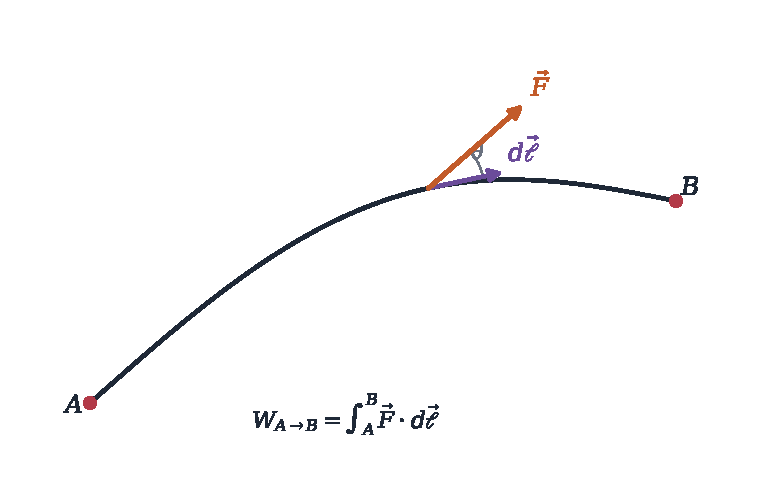
\includegraphics[width=0.74\textwidth]{figures/18_work_path.pdf}
\caption{Curvilinear trajectory $\mathcal{C}$ between states $A$ and $B$. The elementary work $\delta W = \vec{F}\cdot\dd\vec{r} = F_t\,\dd s$ represents the projection of the instantaneous force along the tangential unit vector $\utt$ multiplied by the arc length element $\dd s$.}
\label{fig:work_path}
\end{figure}

In different coordinate systems, the elementary work assumes distinctive explicit forms:
\begin{itemize}[leftmargin=1.5em,itemsep=4pt]
  \item \textbf{Cartesian coordinates:} With $\vec{F} = F_x\,\ihat + F_y\,\jhat + F_z\,\khat$ and $\dd\vec{r} = \dd x\,\ihat + \dd y\,\jhat + \dd z\,\khat$:
  \begin{equation}
  \delta W = F_x\,\dd x + F_y\,\dd y + F_z\,\dd z.
  \end{equation}
  \item \textbf{Frenet-Serret intrinsic coordinates:} Decomposing $\vec{F} = F_t\,\utt + F_n\,\un + F_b\,\ub$ and noting that $\dd\vec{r} = \utt\,\dd s$:
  \begin{equation}
  \delta W = (F_t\,\utt + F_n\,\un + F_b\,\ub) \cdot \utt\,\dd s = F_t\,\dd s.
  \end{equation}
  \emph{Key physical insight:} Normal and binormal forces ($\vec{F}_\perp = F_n\un + F_b\ub$) perform strictly zero mechanical work at every instant because they are perpendicular to the velocity vector $\vec{v} = \dot{s}\utt$.
  \item \textbf{Plane polar coordinates:} With $\vec{F} = F_r\,\ur + F_\theta\,\ut$ and $\dd\vec{r} = \dd r\,\ur + r\,\dd\theta\,\ut$:
  \begin{equation}
  \delta W = F_r\,\dd r + F_\theta\,r\,\dd\theta.
  \end{equation}
\end{itemize}

\begin{definitionbox}{Total Work Along a Finite Trajectory}
The total work performed by a force field $\vec{F}$ as the particle moves along a prescribed continuous path $\mathcal{C}$ from initial point $A$ to final point $B$ is the curvilinear line integral:
\begin{equation}
W_{A \to B} \eqdef \int_{\mathcal{C},\, A}^B \vec{F} \cdot \dd\vec{r} = \int_{t_A}^{t_B} \vec{F}(t) \cdot \vec{v}(t)\,\dd t.
\end{equation}
\end{definitionbox}

Depending on the sign of the scalar product $\vec{F}\cdot\dd\vec{r} = F\,\dd s\,\cos\alpha$:
\begin{enumerate}[leftmargin=1.4em,itemsep=3pt]
  \item \textbf{Motive work ($W > 0$):} $0 \le \alpha < \pi/2$. The force accelerates the particle and increases its kinetic energy.
  \item \textbf{Resistive work ($W < 0$):} $\pi/2 < \alpha \le \pi$. The force opposes motion and drains kinetic energy (e.g., dynamic friction, aerodynamic drag).
  \item \textbf{Zero work ($W = 0$):} $\alpha = \pi/2$. The force is orthogonal to displacement at all times (e.g., normal reaction of a frictionless surface, tension in an inextensible fixed pendulum, magnetic Lorentz force $\vec{F} = q(\vec{v}\times\vec{B})$).
\end{enumerate}

\section{Instantaneous and Average Power}

While work quantifies the cumulative energy delivered over a trajectory, engineering applications demand knowledge of the \textbf{rate} at which energy is transferred.

\begin{definitionbox}{Mechanical Power}
The \textbf{instantaneous power} $\mathcal{P}(t)$ delivered by a force $\vec{F}$ acting on a particle moving with velocity $\vec{v}$ is the time derivative of work:
\begin{equation}
\mathcal{P}(t) \eqdef \frac{\delta W}{\dd t} = \vec{F} \cdot \frac{\dd\vec{r}}{\dd t} = \vec{F} \cdot \vec{v}.
\end{equation}
The SI unit of power is the \textbf{watt} ($\mathrm{W}$), defined as $1\ \mathrm{W} = 1\ \mathrm{J\cdot s^{-1}} = 1\ \mathrm{kg\cdot m^2\cdot s^{-3}}$.
\end{definitionbox}

The average power over a finite time interval $\Delta t = t_B - t_A$ is the ratio of total work to elapsed time:
\begin{equation}
\langle \mathcal{P} \rangle \eqdef \frac{W_{A \to B}}{\Delta t} = \frac{1}{t_B - t_A} \int_{t_A}^{t_B} \mathcal{P}(t)\,\dd t.
\end{equation}

\begin{historicalbox}{James Prescott Joule and the Mechanical Equivalent of Heat}
\begin{minipage}{0.28\textwidth}
\centering
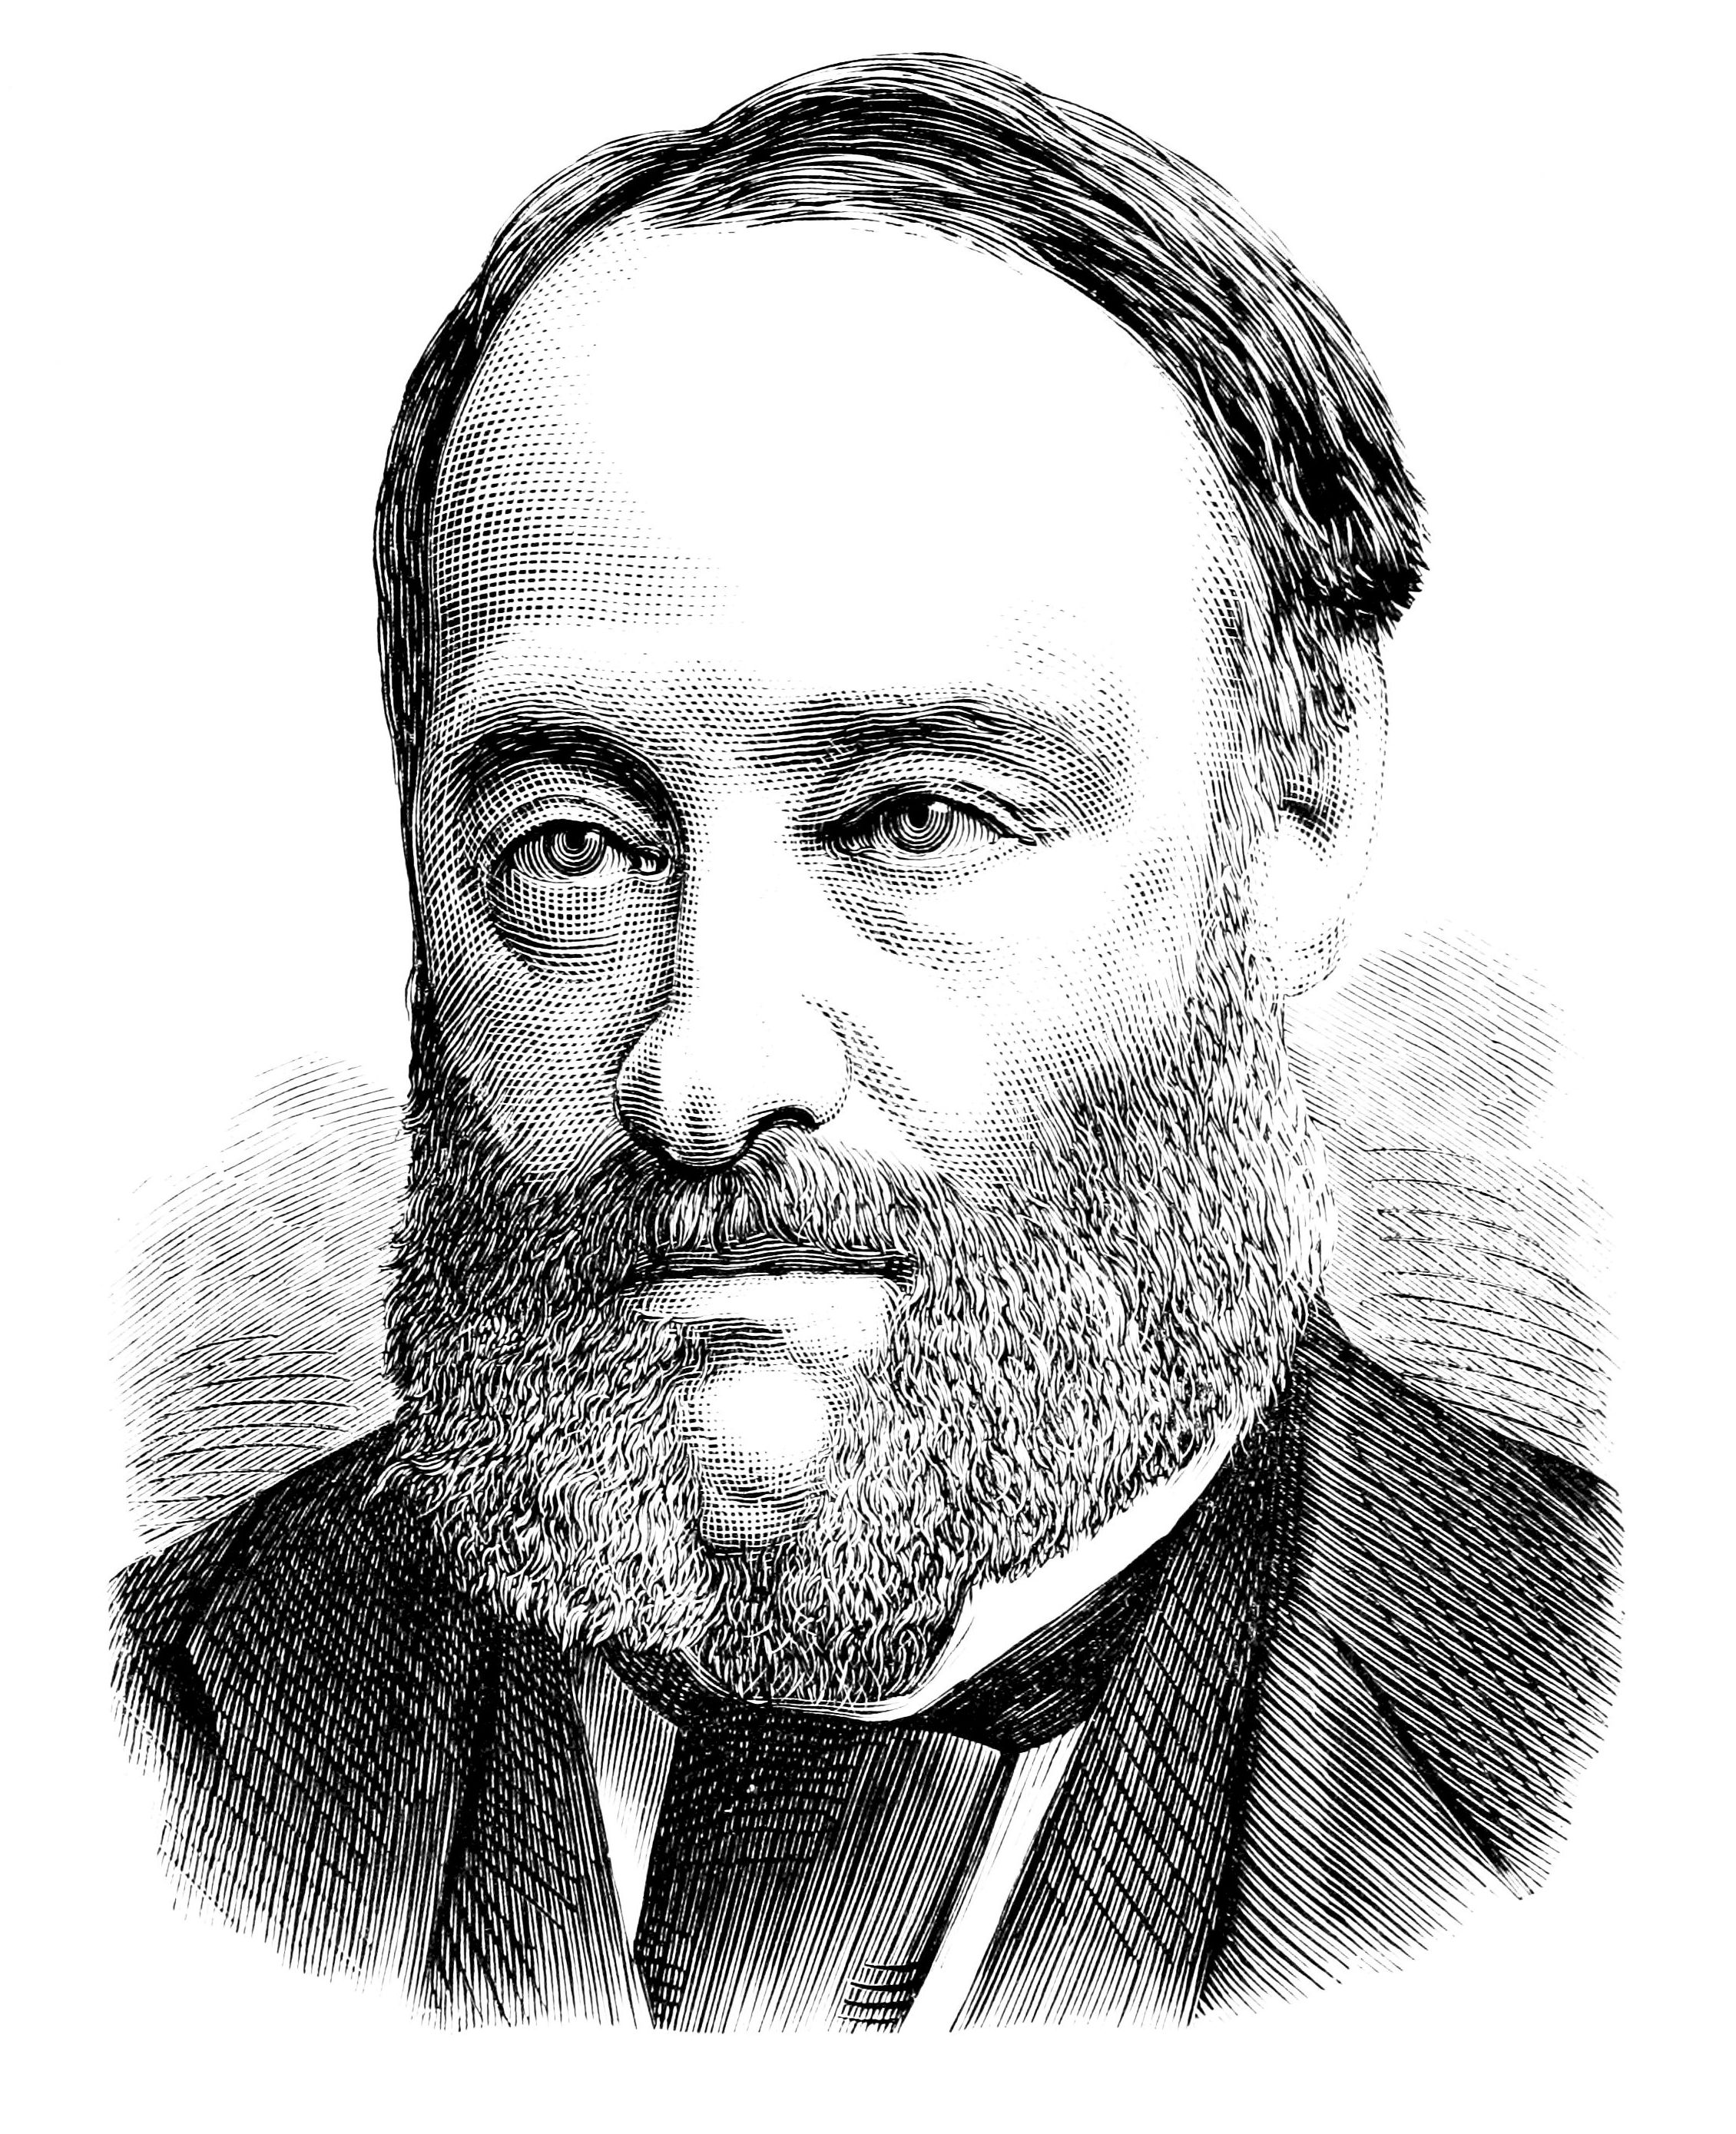
\includegraphics[width=0.92\textwidth]{images/joule.jpg}
\captionof{figure}{James Prescott Joule (1818--1889), portrait by John Collier (1882).}
\end{minipage}\hfill
\begin{minipage}{0.68\textwidth}
In the 1840s, the English physicist and brewer James Prescott Joule conducted meticulous experiments using falling weights to drive paddle wheels immersed in thermally insulated water tanks. 

By measuring the precise mechanical work performed by the descending weights ($\Delta W = mgh$) and the resulting infinitesimal temperature rise of the water, Joule established that mechanical work and thermal energy are interchangeable manifestations of a single universal quantity: \textbf{energy}. His canonical value ($4.18\ \mathrm{J\cdot cal^{-1}}$) shattered the caloric fluid theory and laid the empirical foundation for the First Law of Thermodynamics and the principle of conservation of energy.
\end{minipage}
\end{historicalbox}

\section{Kinetic Energy and the Work-Energy Theorem}

We now establish the mathematical connection between the total work done by all forces and the kinematic state of the particle.

\begin{definitionbox}{Kinetic Energy of a Material Point}
The \textbf{kinetic energy} $E_k$ (also denoted $K$ or $T$) of a point particle of inertial mass $m$ moving at speed $v = \norm{\vec{v}}$ in an inertial reference frame $\mathcal{R}$ is defined as:
\begin{equation}
E_k \eqdef \frac{1}{2} m v^2 = \frac{1}{2} m (\vec{v} \cdot \vec{v}) = \frac{\norm{\vec{p}}^2}{2m}.
\end{equation}
Kinetic energy is an intrinsically positive scalar quantity ($E_k \ge 0$), vanishing if and only if the particle is instantaneously at rest in $\mathcal{R}$.
\end{definitionbox}

\begin{lawbox}{The Work-Energy Theorem (Kinetic Energy Theorem)}
In an inertial frame of reference $\mathcal{R}$, the change in kinetic energy of a material point between any two positions $A$ and $B$ along its trajectory equals the algebraic sum of the work performed by \textbf{all} forces (conservative, non-conservative, internal, and external) acting on the particle:
\begin{equation}
\Delta E_k = E_k(B) - E_k(A) = W_{A \to B}^{\text{net}} = \sum_i W_{A \to B}(\vec{F}_i).
\end{equation}
In differential form, the instantaneous rate of change of kinetic energy equals the net instantaneous power:
\begin{equation}
\frac{\dd E_k}{\dd t} = \mathcal{P}_{\text{net}}(t) = \vec{F}_{\text{net}} \cdot \vec{v}.
\end{equation}
\end{lawbox}

\paragraph{First-Principles Mathematical Proof.}
Let $\vec{F}_{\text{net}} = \sum_i \vec{F}_i$. According to Newton's second law, $\vec{F}_{\text{net}} = m \frac{\dd\vec{v}}{\dd t}$. Differentiating the scalar kinetic energy with respect to time yields:
\[
\frac{\dd E_k}{\dd t} = \frac{\dd}{\dd t}\left(\frac{1}{2} m \vec{v}\cdot\vec{v}\right) = \frac{1}{2}m\left( \frac{\dd\vec{v}}{\dd t}\cdot\vec{v} + \vec{v}\cdot\frac{\dd\vec{v}}{\dd t} \right) = m \vec{v}\cdot\frac{\dd\vec{v}}{\dd t}.
\]
Substituting Newton's law $m\,\dd\vec{v}/\dd t = \vec{F}_{\text{net}}$:
\[
\frac{\dd E_k}{\dd t} = \vec{F}_{\text{net}} \cdot \vec{v} = \mathcal{P}_{\text{net}}(t).
\]
Multiplying by $\dd t$ yields the differential identity $\dd E_k = \vec{F}_{\text{net}}\cdot\dd\vec{r} = \delta W_{\text{net}}$. Integrating both sides along the trajectory from $t_A$ to $t_B$ gives:
\[
\int_{A}^B \dd E_k = E_k(B) - E_k(A) = \int_{A}^B \vec{F}_{\text{net}} \cdot \dd\vec{r} = W_{A \to B}^{\text{net}},
\]
completing the rigorous proof. $\blacksquare$

\subsection{Work-Energy Theorem in Non-Inertial Frames}

In a non-inertial frame of reference $\mathcal{R}'$, Newton's second law includes inertial fictitious forces:
\[
m\vec{a}_r = \vec{F}_{\text{real}} + \vec{F}_{\text{ie}} + \vec{F}_{\text{ic}},
\]
where $\vec{F}_{\text{ie}} = -m\vec{a}_e$ is the entrainment force and $\vec{F}_{\text{ic}} = -2m(\vec{\Omega}\times\vec{v}_r)$ is the Coriolis force.

Projecting onto the relative velocity $\vec{v}_r$:
\[
\frac{\dd E_k'}{\dd t} = m\vec{v}_r \cdot \vec{a}_r = \vec{F}_{\text{real}} \cdot \vec{v}_r + \vec{F}_{\text{ie}} \cdot \vec{v}_r + \vec{F}_{\text{ic}} \cdot \vec{v}_r.
\]
Crucially, the Coriolis force is identically perpendicular to the relative velocity:
\[
\vec{F}_{\text{ic}} \cdot \vec{v}_r = -2m (\vec{\Omega} \times \vec{v}_r) \cdot \vec{v}_r \equiv 0.
\]
\begin{lawbox}{Work of Inertial Forces}
The Coriolis force performs \textbf{strictly zero mechanical work} in all non-inertial frames:
\begin{equation}
\mathcal{P}_{\text{Coriolis}} \equiv 0, \qquad W_{\text{Coriolis}} \equiv 0.
\end{equation}
The Work-Energy theorem in a non-inertial frame $\mathcal{R}'$ reads:
\begin{equation}
\Delta E_k' = W^{\text{real}} + W_{\text{ie}},
\end{equation}
where $W_{\text{ie}} = \int \vec{F}_{\text{ie}}\cdot\dd\vec{r}'$ is the work of entrainment forces (e.g., the centrifugal force).
\end{lawbox}

\begin{cautionbox}[Common Pitfall: The Inexactness of Work]
Never write ``$\Delta W = W_B - W_A$''. Work is \emph{not} a property possessed by a body. A body possesses mass, momentum, and energy, but it \emph{does not} possess work. Work is an energy flux in transit across the system boundary during a process. The notation $W_{A\to B}$ denotes the integrated integral along a specified path.
\end{cautionbox}

\section{Comprehensive Worked Examples}

\begin{workedexample}{The Vertical Loop-the-Loop Roller Coaster}
A small block of mass $m$ slides from rest down a frictionless track that terminates in a circular vertical loop of radius $R$. The block is released from an initial height $h$ above the lowest point of the track $O$. Gravity $\vec{g} = -g\,\khat$ acts vertically downward.
\begin{enumerate}[leftmargin=1.4em,itemsep=3pt]
  \item Determine the speed $v(\theta)$ and the normal reaction force $N(\theta)$ exerted by the track as a function of the polar angle $\theta \in [0, \pi]$ measured from the bottom of the loop.
  \item Find the critical minimum release height $h_{\min}$ required for the block to negotiate the entire loop without losing contact with the track.
  \item Calculate the normal contact force experienced at the lowest point $\theta = 0$ when released from $h = h_{\min}$.
\end{enumerate}

\paragraph{Solution.}
\textbf{1. Speed and Normal Force via Work-Energy Theorem:}\\
Between the release point (height $h$, speed $v_0 = 0$) and an arbitrary position on the loop at angle $\theta$, the height above the bottom is:
\[
z(\theta) = R(1 - \cos\theta).
\]
The forces acting on the block are the weight $\vec{P} = m\vec{g}$ and the track normal reaction $\vec{N} = -N(\theta)\,\ur$ directed inward toward the center. Because the track is frictionless, the normal force is orthogonal to the displacement at every point: $\vec{N}\cdot\dd\vec{r} = 0$, so $W(\vec{N}) = 0$.

The work done by gravity as the particle descends from $z_1 = h$ to $z_2 = z(\theta)$ is:
\[
W(\vec{P}) = -mg\,\Delta z = mg\left(h - R(1 - \cos\theta)\right).
\]
Applying the Work-Energy Theorem $\Delta E_k = W_{\text{net}}$:
\[
\frac{1}{2} m v(\theta)^2 - 0 = mg\left(h - R(1 - \cos\theta)\right) \implies v^2(\theta) = 2g\left(h - R(1 - \cos\theta)\right).
\]
To find the normal contact force $N(\theta)$, we project Newton's second law onto the inward normal unit vector $\un = -\ur$ in the Frenet frame:
\[
\sum F_n = m a_n \implies N(\theta) - mg\cos\theta = m \frac{v^2(\theta)}{R}.
\]
Substituting the expression for $v^2(\theta)$:
\[
N(\theta) = mg\cos\theta + \frac{m}{R}\left[ 2g(h - R + R\cos\theta) \right] = \frac{mg}{R}\left( 2h - 2R + 3R\cos\theta \right).
\]

\textbf{2. Critical Release Height $h_{\min}$:}\\
For the block to remain in continuous contact with the track, the normal reaction must remain non-negative: $N(\theta) \ge 0$ for all $\theta \in [0, \pi]$. Since $\cos\theta$ is monotonically decreasing from $+1$ to $-1$, $N(\theta)$ attains its global minimum at the apex of the loop ($\theta = \pi$, where $\cos\pi = -1$):
\[
N(\pi) = \frac{mg}{R}\left( 2h - 2R - 3R \right) = \frac{mg}{R}(2h - 5R).
\]
The threshold of detachment occurs when $N(\pi) = 0$:
\[
2h_{\min} - 5R = 0 \implies h_{\min} = \frac{5}{2}R = 2.5\,R.
\]
At this critical height, the speed at the summit is $v_{\text{top}} = \sqrt{2g(2.5R - 2R)} = \sqrt{gR}$, exactly balancing centrifugal effect and gravity ($g = v^2/R$).

\textbf{3. Normal Force at the Lowest Point:}\\
Evaluating $N(0)$ with $\theta = 0$ ($\cos 0 = 1$) and $h = \frac{5}{2}R$:
\[
N(0) = \frac{mg}{R}\left( 2\left(\frac{5}{2}R\right) - 2R + 3R \right) = \frac{mg}{R}(5R - 2R + 3R) = 6mg.
\]
The track must exert a normal force equal to \textbf{six times} the body's resting weight at the bottom of the loop to simultaneously support gravity and provide the necessary centripetal acceleration.
\end{workedexample}

\begin{workedexample}{Detachment from a Frictionless Spherical Dome}
A small ice pellet of mass $m$ rests at the apex of a fixed frictionless spherical dome of radius $R$. Given an infinitesimal nudge, it slides down the dome under gravity.
\begin{enumerate}[leftmargin=1.4em,itemsep=3pt]
  \item Derive the speed of the pellet as a function of the polar angle $\theta$ measured from the vertical apex.
  \item Compute the normal contact force $N(\theta)$ exerted by the dome.
  \item Determine the exact polar angle $\theta_{\text{detach}}$, the height $z_{\text{detach}}$, and the velocity at the instant the pellet flies off the surface.
\end{enumerate}

\paragraph{Solution.}
\textbf{1. Speed via Work-Energy Theorem:}\\
Placing the origin at the center of the sphere, the apex is at vertical coordinate $z_0 = R$. At polar angle $\theta$, the vertical height is $z(\theta) = R\cos\theta$.

Since the dome is frictionless, $\vec{N} = N(\theta)\,\ur$ is purely radial and perpendicular to the displacement $\dd\vec{r} = R\,\dd\theta\,\ut$. Thus $W(\vec{N}) = 0$.
The work done by gravity during the descent from $z_0 = R$ to $z(\theta) = R\cos\theta$ is:
\[
W(\vec{P}) = -mg\,\Delta z = mg(R - R\cos\theta) = mgR(1 - \cos\theta).
\]
By the Work-Energy Theorem, assuming an infinitesimal initial speed $v_0 \to 0$:
\[
\frac{1}{2}mv^2 - 0 = mgR(1 - \cos\theta) \implies v(\theta) = \sqrt{2gR(1 - \cos\theta)}.
\]

\textbf{2. Normal Contact Force:}\\
In plane polar coordinates with basis $(\ur, \ut)$, the forces are:
\[
\vec{P} = mg\cos\theta\,\ur - mg\sin\theta\,\ut, \qquad \vec{N} = N(\theta)\,\ur.
\]
The radial equation of motion (projecting along $-\ur$, directed toward the center) is:
\[
\sum F_{\text{inward}} = mg\cos\theta - N(\theta) = m a_n = m \frac{v^2}{R}.
\]
Substituting $v^2 = 2gR(1 - \cos\theta)$:
\[
N(\theta) = mg\cos\theta - \frac{m}{R}\left[ 2gR(1 - \cos\theta) \right] = mg(3\cos\theta - 2).
\]

\textbf{3. Angle, Height, and Speed at Detachment:}\\
The dome cannot pull on the pellet; it can only push ($N(\theta) \ge 0$). Detachment occurs precisely when the contact force vanishes, $N(\theta_{\text{detach}}) = 0$:
\[
3\cos\theta_{\text{detach}} - 2 = 0 \implies \cos\theta_{\text{detach}} = \frac{2}{3}.
\]
The exact detachment angle is:
\[
\theta_{\text{detach}} = \arccos\left(\frac{2}{3}\right) \approx 48.19^\circ \approx 0.8411\ \mathrm{rad}.
\]
The height of detachment above the base of the hemisphere is:
\[
z_{\text{detach}} = R\cos\theta_{\text{detach}} = \frac{2}{3}R.
\]
The pellet has fallen through a vertical drop of $\Delta z = R - \frac{2}{3}R = \frac{1}{3}R$.
Its speed at the instant of detachment is:
\[
v_{\text{detach}} = \sqrt{2gR\left(1 - \frac{2}{3}\right)} = \sqrt{\frac{2}{3}gR}.
\]
For all subsequent motion $\theta > \theta_{\text{detach}}$, the pellet executes a free projectile parabolic trajectory in vacuum.
\end{workedexample}

\begin{workedexample}{Power Requirements and Acceleration with Aerodynamic Drag}
A sports car of mass $m = 1200\ \mathrm{kg}$ accelerates along a straight horizontal track. The internal combustion engine delivers a constant mechanical power $\mathcal{P}_0 = 180\ \mathrm{kW}$ to the drive wheels. The vehicle encounters an aerodynamic drag force modeled by $F_d = \frac{1}{2} C_d A \rho v^2 = \beta v^2$, where the aerodynamic factor is $\beta = 0.45\ \mathrm{kg\cdot m^{-1}}$.
\begin{enumerate}[leftmargin=1.4em,itemsep=3pt]
  \item Determine the terminal maximum speed $v_{\max}$ of the vehicle.
  \item Formulate the differential equation governing speed $v(t)$ using the Work-Energy theorem (power formulation).
  \item Derive an expression for the distance $x$ required to accelerate from an initial speed $v_1 = 10\ \mathrm{m\cdot s^{-1}}$ to $v_2 = 30\ \mathrm{m\cdot s^{-1}}$.
\end{enumerate}

\paragraph{Solution.}
\textbf{1. Maximum Terminal Speed:}\\
At terminal speed $v_{\max}$, the vehicle is no longer accelerating ($\dd v/\dd t = 0$). By the power formulation of the Work-Energy theorem:
\[
\frac{\dd E_k}{\dd t} = \mathcal{P}_{\text{net}} = \mathcal{P}_{\text{engine}} - \mathcal{P}_{\text{drag}} = 0.
\]
The rate of dissipation by aerodynamic drag is $\mathcal{P}_{\text{drag}} = F_d v = \beta v^3$. Equating engine power to drag power:
\[
\mathcal{P}_0 = \beta v_{\max}^3 \implies v_{\max} = \left(\frac{\mathcal{P}_0}{\beta}\right)^{1/3}.
\]
Plugging in numerical values:
\[
v_{\max} = \left( \frac{180 \times 10^3\ \mathrm{W}}{0.45\ \mathrm{kg\cdot m^{-1}}} \right)^{1/3} = (400\,000)^{1/3} \approx 73.68\ \mathrm{m\cdot s^{-1}} \approx 265.2\ \mathrm{km\cdot h^{-1}}.
\]

\textbf{2. Differential Equation of Motion:}\\
The net power is $\mathcal{P}_{\text{net}} = \mathcal{P}_0 - \beta v^3$. Since $E_k = \frac{1}{2}mv^2$, we have $\frac{\dd E_k}{\dd t} = mv\frac{\dd v}{\dd t}$. Therefore:
\[
mv \frac{\dd v}{\dd t} = \mathcal{P}_0 - \beta v^3 \implies \frac{\dd v}{\dd t} = \frac{\mathcal{P}_0 - \beta v^3}{mv}.
\]

\textbf{3. Distance to Accelerate from $v_1$ to $v_2$:}\\
To find distance $x$ as a function of speed, we employ the kinematic chain rule $\frac{\dd v}{\dd t} = v\frac{\dd v}{\dd x}$:
\[
mv^2 \frac{\dd v}{\dd x} = \mathcal{P}_0 - \beta v^3 \implies \dd x = \frac{m v^2\,\dd v}{\mathcal{P}_0 - \beta v^3}.
\]
Notice the remarkable substitution: let $u = \mathcal{P}_0 - \beta v^3$. Then $\dd u = -3\beta v^2\,\dd v$, so $v^2\,\dd v = -\frac{\dd u}{3\beta}$.
Integrating from $x = 0$ ($v = v_1$) to $x$ ($v = v_2$):
\[
x = \int_{v_1}^{v_2} \frac{m v^2\,\dd v}{\mathcal{P}_0 - \beta v^3} = -\frac{m}{3\beta} \int_{u_1}^{u_2} \frac{\dd u}{u} = \frac{m}{3\beta} \ln\left( \frac{\mathcal{P}_0 - \beta v_1^3}{\mathcal{P}_0 - \beta v_2^3} \right).
\]
Substituting the numerical values:
\[
u_1 = 180\,000 - 0.45(10)^3 = 180\,000 - 450 = 179\,550\ \mathrm{W},
\]
\[
u_2 = 180\,000 - 0.45(30)^3 = 180\,000 - 12\,150 = 167\,850\ \mathrm{W}.
\]
The required acceleration distance is:
\[
x = \frac{1200}{3(0.45)} \ln\left(\frac{179\,550}{167\,850}\right) = \frac{1200}{1.35} \ln(1.0697) \approx 888.89 \times 0.06738 \approx 59.9\ \mathrm{m}.
\]
The scalar power formulation resolved in three lines an integration that would have required difficult vector algebra.
\end{workedexample}

\chapter{Conservative Forces and Potential Energy}
\label{ch:potential_energy}

\begin{chapterintro}
\textbf{Chapter Objectives:} In this chapter, we develop the theoretical foundation of potential energy. You will formulate the mathematical criteria for conservative vector fields via curl and path independence; derive the potential energy function $E_p$ from gradient relations; prove the Theorem of Mechanical Energy Conservation; and calculate energy dissipation by non-conservative forces in complex mechanical and gravitational systems.
\end{chapterintro}

\section{Conservative Vector Fields and Path Independence}

In the preceding chapter, we established that the work done by a force along a path $\mathcal{C}$ between two points $A$ and $B$ generally depends on the specific geometric path traversed. However, a profoundly important class of physical forces possesses a special property: the work performed is entirely independent of the trajectory connecting the initial and final states.

\begin{definitionbox}{Conservative Force Field}
A force field $\vec{F}(\vec{r})$ defined on an open, connected domain $\mathcal{D} \subseteq \mathbb{R}^3$ is said to be \textbf{conservative} if the mechanical work performed along any smooth curve $\mathcal{C}$ joining point $A$ to point $B$ depends solely on the positions of the endpoints $A$ and $B$, and not on the particular path taken:
\begin{equation}
W_{A \to B}^{(\mathcal{C}_1)} = W_{A \to B}^{(\mathcal{C}_2)} = \int_A^B \vec{F} \cdot \dd\vec{r}, \qquad \forall\, \mathcal{C}_1, \mathcal{C}_2 \subset \mathcal{D}.
\end{equation}
\end{definitionbox}

An immediate and mathematically equivalent characterization concerns closed loops. Let $\mathcal{C}$ be any closed contour ($\oint$) beginning and ending at the same point:
\begin{lawbox}{Closed-Loop Criterion for Conservative Forces}
A force field $\vec{F}$ is conservative if and only if its circulation around every closed closed curve $\mathcal{C}$ in $\mathcal{D}$ vanishes identically:
\begin{equation}
\oint_{\mathcal{C}} \vec{F} \cdot \dd\vec{r} \equiv 0.
\end{equation}
\end{lawbox}

\paragraph{Proof of Equivalence.}
Let $A$ and $B$ be two arbitrary points on a closed loop $\mathcal{C}$. Decompose $\mathcal{C}$ into two forward paths: $\mathcal{C}_1$ from $A$ to $B$, and $\mathcal{C}_2$ from $B$ to $A$ (or $-\mathcal{C}_2$ from $A$ to $B$). Then:
\[
\oint_{\mathcal{C}} \vec{F}\cdot\dd\vec{r} = \int_{\mathcal{C}_1} \vec{F}\cdot\dd\vec{r} + \int_{\mathcal{C}_2} \vec{F}\cdot\dd\vec{r} = \int_{\mathcal{C}_1} \vec{F}\cdot\dd\vec{r} - \int_{-\mathcal{C}_2} \vec{F}\cdot\dd\vec{r}.
\]
This integral vanishes for all contours if and only if $\int_{\mathcal{C}_1} \vec{F}\cdot\dd\vec{r} = \int_{-\mathcal{C}_2} \vec{F}\cdot\dd\vec{r}$, which is precisely path independence. $\blacksquare$

\section{Differential Criteria: The Curl Condition}

From Stokes' theorem in vector calculus, the circulation of a differentiable vector field along the boundary $\partial S$ of an orientable surface $S$ is related to the flux of its curl:
\begin{equation}
\oint_{\partial S} \vec{F} \cdot \dd\vec{r} = \iint_S (\vec{\nabla} \times \vec{F}) \cdot \dd\vec{S}.
\end{equation}

\begin{lawbox}{The Curl Condition for Conservative Fields}
In a simply connected spatial domain $\mathcal{D}$, a continuously differentiable force field $\vec{F}(\vec{r})$ is conservative if and only if its curl (rotational) vanishes identically everywhere:
\begin{equation}
\vec{\nabla} \times \vec{F} = \rot\vec{F} \equiv \vzero.
\end{equation}
In Cartesian coordinates, this condition is equivalent to the three scalar component relations:
\begin{equation}
\frac{\partial F_z}{\partial y} = \frac{\partial F_y}{\partial z}, \qquad \frac{\partial F_x}{\partial z} = \frac{\partial F_z}{\partial x}, \qquad \frac{\partial F_y}{\partial x} = \frac{\partial F_x}{\partial y}.
\end{equation}
\end{lawbox}

\begin{itemize}[leftmargin=1.5em,itemsep=4pt]
  \item \textbf{Example of a Conservative Field:} A central force field $\vec{F}(\vec{r}) = f(r)\,\ur$. As proven in Chapter 2, $\vec{\nabla}\times(f(r)\ur) = \vzero$ identically for any scalar function $f(r)$. Hence, all spherically symmetric central forces (Newtonian gravity, Coulomb electrostatics) are conservative.
  \item \textbf{Example of a Non-Conservative Field:} A 2D rotational vortex field $\vec{F} = -y\,\ihat + x\,\jhat$.
  \[
  \vec{\nabla}\times\vec{F} = \left(\frac{\partial F_y}{\partial x} - \frac{\partial F_x}{\partial y}\right)\khat = (1 - (-1))\khat = 2\,\khat \neq \vzero.
  \]
  Integrating around a unit circle $\mathcal{C}$ gives $\oint \vec{F}\cdot\dd\vec{r} = 2\pi \neq 0$.
  \item \textbf{Frictional Forces:} Kinetic friction $\vec{F}_f = -\mu_k N \frac{\vec{v}}{v}$ is directed opposite to velocity at every instant. The circulation around a closed path of perimeter $L$ is $\oint \vec{F}_f\cdot\dd\vec{r} = \oint (-\mu_k N)\,\dd s = -\mu_k N L < 0$. Mechanical energy is irreversibly dissipated into microscopic thermal vibrations.
\end{itemize}

\section{The Potential Energy Function}

Because the work done by a conservative force between a fixed reference point $O$ and an arbitrary point $M$ depends only on the position of $M$, we can define a scalar state function:

\begin{definitionbox}{Potential Energy Function}
Let $\vec{F}(\vec{r})$ be a conservative force field. The \textbf{potential energy} $E_p(\vec{r})$ (or $U(\vec{r})$) associated with $\vec{F}$ is defined such that the elementary work is the exact negative differential of $E_p$:
\begin{equation}
\delta W = \vec{F} \cdot \dd\vec{r} \eqdef -\dd E_p.
\end{equation}
Integrating from an arbitrary reference configuration $\vec{r}_{\text{ref}}$ (where $E_p(\vec{r}_{\text{ref}}) = 0$ by convention):
\begin{equation}
E_p(\vec{r}) \eqdef -\int_{\vec{r}_{\text{ref}}}^{\vec{r}} \vec{F} \cdot \dd\vec{r}'.
\end{equation}
\end{definitionbox}

\begin{lawbox}{Gradient Relation Between Force and Potential Energy}
A conservative force is the negative spatial gradient of its potential energy:
\begin{equation}
\vec{F} = -\vec{\nabla} E_p = -\grad E_p.
\end{equation}
\begin{itemize}[leftmargin=1.5em,itemsep=3pt]
  \item \textbf{Cartesian coordinates:} $\vec{F} = -\left( \frac{\partial E_p}{\partial x}\ihat + \frac{\partial E_p}{\partial y}\jhat + \frac{\partial E_p}{\partial z}\khat \right)$.
  \item \textbf{Cylindrical coordinates:} $\vec{F} = -\left( \frac{\partial E_p}{\partial r}\ur + \frac{1}{r}\frac{\partial E_p}{\partial \theta}\ut + \frac{\partial E_p}{\partial z}\khat \right)$.
  \item \textbf{Spherical coordinates:} $\vec{F} = -\left( \frac{\partial E_p}{\partial r}\ur + \frac{1}{r}\frac{\partial E_p}{\partial \theta}\ut + \frac{1}{r\sin\theta}\frac{\partial E_p}{\partial \phi}\uphi \right)$.
\end{itemize}
\end{lawbox}

The negative sign has profound physical significance: \textbf{a conservative force always points in the direction of steepest descent of the potential energy landscape}. A particle naturally seeks to minimize its potential energy.

\subsection{Canonical Potential Energy Expressions}

\begin{table}[htbp]
\centering
\renewcommand{\arraystretch}{1.35}
\begin{tabular}{@{}llll@{}}
\toprule
\textbf{Interaction} & \textbf{Force Law $\vec{F}(\vec{r})$} & \textbf{Potential Energy $E_p(\vec{r})$} & \textbf{Reference Zero} \\
\midrule
Uniform Gravity & $\vec{P} = -mg\,\khat$ & $E_p(z) = mgz + C$ & $E_p(0) = 0$ at $z = 0$ \\
Hooke's Spring & $\vec{F} = -k(x - x_0)\,\ihat$ & $E_p(x) = \frac{1}{2}k(x - x_0)^2$ & $E_p(x_0) = 0$ at equilibrium \\
Newtonian Gravitation & $\vec{F} = -\frac{G M m}{r^2}\,\ur$ & $E_p(r) = -\frac{G M m}{r}$ & $E_p(\infty) = 0$ at infinity \\
Coulomb Electrostatics & $\vec{F} = \frac{q_1 q_2}{4\pi\varepsilon_0 r^2}\,\ur$ & $E_p(r) = \frac{q_1 q_2}{4\pi\varepsilon_0 r}$ & $E_p(\infty) = 0$ at infinity \\
\bottomrule
\end{tabular}
\caption{Fundamental conservative forces of classical mechanics and their standard potential energy functions.}
\label{tab:potentials}
\end{table}

\section{The Principle of Conservation of Mechanical Energy}

\begin{definitionbox}{Total Mechanical Energy}
The \textbf{total mechanical energy} $E_m$ of a material point is the sum of its kinetic energy and all its potential energies:
\begin{equation}
E_m \eqdef E_k + E_p = \frac{1}{2}m v^2 + E_p(\vec{r}).
\end{equation}
\end{definitionbox}

Decomposing the net force acting on a particle into conservative and non-conservative components, $\vec{F}_{\text{net}} = \vec{F}_{\text{c}} + \vec{F}_{\text{nc}}$, we take the time derivative of $E_m$:
\[
\frac{\dd E_m}{\dd t} = \frac{\dd E_k}{\dd t} + \frac{\dd E_p}{\dd t}.
\]
From the Work-Energy Theorem, $\frac{\dd E_k}{\dd t} = (\vec{F}_{\text{c}} + \vec{F}_{\text{nc}})\cdot\vec{v}$. Using the chain rule for $E_p(\vec{r}(t))$:
\[
\frac{\dd E_p}{\dd t} = \vec{\nabla} E_p \cdot \frac{\dd\vec{r}}{\dd t} = -\vec{F}_{\text{c}} \cdot \vec{v}.
\]
Adding these two expressions:
\[
\frac{\dd E_m}{\dd t} = (\vec{F}_{\text{c}} + \vec{F}_{\text{nc}})\cdot\vec{v} - \vec{F}_{\text{c}}\cdot\vec{v} = \vec{F}_{\text{nc}} \cdot \vec{v} = \mathcal{P}_{\text{nc}}.
\]

\begin{lawbox}{Theorem of Mechanical Energy}
The rate of change of mechanical energy equals the instantaneous power delivered by non-conservative forces:
\begin{equation}
\frac{\dd E_m}{\dd t} = \vec{F}_{\text{nc}} \cdot \vec{v} = \mathcal{P}_{\text{nc}}.
\end{equation}
Over a finite trajectory between states $A$ and $B$:
\begin{equation}
\Delta E_m = E_m(B) - E_m(A) = W_{A \to B}^{\text{nc}} = \int_A^B \vec{F}_{\text{nc}} \cdot \dd\vec{r}.
\end{equation}
\textbf{Corollary (Conservation of Mechanical Energy):} If all forces performing work on the system are conservative ($W^{\text{nc}} = 0$), the total mechanical energy is an invariant of motion:
\begin{equation}
E_m = E_k + E_p = \text{constant}.
\end{equation}
\end{lawbox}

\section{Comprehensive Worked Examples}

\begin{workedexample}{Escape Velocity from Planetary Gravitation}
A space probe of mass $m$ is launched vertically upward from the surface of a spherical planet of mass $M$ and radius $R$. Atmospheric drag is negligible.
\begin{enumerate}[leftmargin=1.4em,itemsep=3pt]
  \item Determine the maximum altitude $h_{\max}$ reached if the initial launch speed is $v_0$.
  \item Calculate the critical escape velocity $v_{\text{esc}}$ necessary for the probe to permanently overcome the planet's gravitational pull and reach infinity with non-negative kinetic energy.
  \item Evaluate $v_{\text{esc}}$ numerically for Earth ($M_\oplus = 5.972\times 10^{24}\ \mathrm{kg}$, $R_\oplus = 6371\ \mathrm{km}$) and for the Moon ($M_{\text{Moon}} = 7.342\times 10^{22}\ \mathrm{kg}$, $R_{\text{Moon}} = 1737\ \mathrm{km}$).
\end{enumerate}

\paragraph{Solution.}
\textbf{1. Maximum Altitude Reached:}\\
The only force performing work is Newtonian gravitation $\vec{F}_G = -\frac{G M m}{r^2}\ur$, which is conservative with potential energy:
\[
E_p(r) = -\frac{G M m}{r}.
\]
Since no non-conservative forces act, mechanical energy is conserved throughout the trajectory:
\[
E_m = \frac{1}{2}m v(r)^2 - \frac{G M m}{r} = \text{constant}.
\]
At the planetary surface, $r_1 = R$ and $v_1 = v_0$:
\[
E_m = \frac{1}{2}m v_0^2 - \frac{G M m}{R}.
\]
At maximum height $r_{\max} = R + h_{\max}$, the radial velocity drops momentarily to zero ($v = 0$):
\[
E_m = 0 - \frac{G M m}{R + h_{\max}}.
\]
Equating the two energies:
\[
\frac{1}{2}m v_0^2 - \frac{G M m}{R} = -\frac{G M m}{R + h_{\max}}.
\]
Dividing by $m$ and rearranging:
\[
\frac{G M}{R + h_{\max}} = \frac{G M}{R} - \frac{1}{2}v_0^2 = \frac{2GM - R v_0^2}{2R}.
\]
Inverting both sides:
\[
R + h_{\max} = \frac{2GM R}{2GM - R v_0^2} \implies h_{\max} = \frac{R^2 v_0^2}{2GM - R v_0^2}.
\]
Notice that when $v_0 \ll \sqrt{2GM/R}$, using $g = GM/R^2$:
\[
h_{\max} \approx \frac{R^2 v_0^2}{2gR^2} = \frac{v_0^2}{2g},
\]
which perfectly reproduces the uniform-field kinematic result!

\textbf{2. Critical Escape Velocity $v_{\text{esc}}$:}\\
For the probe to reach infinity ($r \to \infty$), its mechanical energy must satisfy $E_m \ge 0$, because at $r \to \infty$, $E_p(\infty) \to 0$ and $E_k(\infty) \ge 0$.
The threshold condition for escape corresponds to $E_m = 0$ (the probe arrives at infinity with speed $v_\infty = 0$):
\[
\frac{1}{2} m v_{\text{esc}}^2 - \frac{G M m}{R} = 0 \implies v_{\text{esc}} = \sqrt{\frac{2GM}{R}} = \sqrt{2gR}.
\]

\textbf{3. Numerical Computations:}\\
Using Newton's gravitational constant $G = 6.6743\times 10^{-11}\ \mathrm{m^3\cdot kg^{-1}\cdot s^{-2}}$:
\begin{itemize}[leftmargin=1.5em,itemsep=3pt]
  \item \textbf{For Earth:}
  \[
  v_{\text{esc},\oplus} = \sqrt{\frac{2(6.6743\times 10^{-11})(5.972\times 10^{24})}{6.371\times 10^6}} = \sqrt{1.2509\times 10^8} \approx 11\,184\ \mathrm{m\cdot s^{-1}} \approx 11.18\ \mathrm{km\cdot s^{-1}}.
  \]
  \item \textbf{For the Moon:}
  \[
  v_{\text{esc},\text{Moon}} = \sqrt{\frac{2(6.6743\times 10^{-11})(7.342\times 10^{22})}{1.737\times 10^6}} = \sqrt{5.642\times 10^6} \approx 2\,375\ \mathrm{m\cdot s^{-1}} \approx 2.38\ \mathrm{km\cdot s^{-1}}.
  \]
\end{itemize}
Because the Moon's escape speed ($2.38\ \mathrm{km/s}$) is comparable to the thermal root-mean-square speed of light atmospheric molecules ($v_{\text{rms}} = \sqrt{3k_B T/m}$), the Moon could not retain an atmosphere over geological timescales.
\end{workedexample}

\begin{workedexample}{Two Collinear Springs and Equilibrium Energy Landscape}
A particle of mass $m$ slides along a frictionless horizontal guide rail ($x$-axis). It is connected to two fixed anchor points $A_1$ (at $x = -L$) and $A_2$ (at $x = +L$) by two ideal linear springs with spring constants $k_1, k_2$ and unextended resting lengths $l_{01}, l_{02}$ respectively.
\begin{enumerate}[leftmargin=1.4em,itemsep=3pt]
  \item Formulate the total potential energy $E_p(x)$ of the system as a function of the position $x \in (-L, L)$.
  \item Find the equilibrium position $x_{\text{eq}}$ where the net force vanishes by setting $\frac{\dd E_p}{\dd x} = 0$.
  \item Determine the effective spring constant $k_{\text{eff}} = \left.\frac{\dd^2 E_p}{\dd x^2}\right|_{x_{\text{eq}}}$ and compute the natural frequency of oscillation $\omega_0$.
\end{enumerate}

\paragraph{Solution.}
\textbf{1. Total Potential Energy:}\\
Spring 1 extends from $A_1(-L)$ to $M(x)$. Its instantaneous length is $l_1 = x - (-L) = x + L$.
The elastic potential energy stored in spring 1 is:
\[
E_{p1}(x) = \frac{1}{2} k_1 (l_1 - l_{01})^2 = \frac{1}{2} k_1 (x + L - l_{01})^2.
\]
Spring 2 extends from $M(x)$ to $A_2(+L)$. Its instantaneous length is $l_2 = L - x$.
The elastic potential energy stored in spring 2 is:
\[
E_{p2}(x) = \frac{1}{2} k_2 (l_2 - l_{02})^2 = \frac{1}{2} k_2 (L - x - l_{02})^2 = \frac{1}{2} k_2 (x - (L - l_{02}))^2.
\]
The total potential energy is the sum:
\[
E_p(x) = \frac{1}{2} k_1 (x + L - l_{01})^2 + \frac{1}{2} k_2 (x - L + l_{02})^2.
\]

\textbf{2. Equilibrium Position:}\\
The net restoring force is $F_x(x) = -\frac{\dd E_p}{\dd x}$. Differentiating:
\[
\frac{\dd E_p}{\dd x} = k_1(x + L - l_{01}) + k_2(x - L + l_{02}) = (k_1 + k_2) x + k_1(L - l_{01}) - k_2(L - l_{02}).
\]
Setting $\frac{\dd E_p}{\dd x} = 0$ yields the unique equilibrium position:
\[
x_{\text{eq}} = \frac{k_2(L - l_{02}) - k_1(L - l_{01})}{k_1 + k_2}.
\]
Notice that if the springs are identical ($k_1 = k_2 = k$ and $l_{01} = l_{02} = l_0$), then $x_{\text{eq}} = 0$, directly at the center as dictated by symmetry.

\textbf{3. Effective Stiffness and Frequency:}\\
Taking the second derivative of the potential energy:
\[
k_{\text{eff}} \eqdef \left.\frac{\dd^2 E_p}{\dd x^2}\right|_{x_{\text{eq}}} = k_1 + k_2.
\]
Since $k_1 > 0$ and $k_2 > 0$, $k_{\text{eff}} = k_1 + k_2 > 0$ strictly; the potential well is parabolic and concave upward everywhere, guaranteeing that $x_{\text{eq}}$ is an unconditionally stable equilibrium.
The angular frequency of small (and even large linear) oscillations about $x_{\text{eq}}$ is:
\[
\omega_0 = \sqrt{\frac{k_{\text{eff}}}{m}} = \sqrt{\frac{k_1 + k_2}{m}}, \qquad T_0 = 2\pi\sqrt{\frac{m}{k_1 + k_2}}.
\]
The two springs act in parallel from a dynamical perspective, reinforcing each other's stiffness.
\end{workedexample}

\begin{workedexample}{Energy Dissipation of a Block on a Rough Incline with a Spring}
A block of mass $m = 2.0\ \mathrm{kg}$ is placed against a compressed spring (stiffness $k = 400\ \mathrm{N\cdot m^{-1}}$, compression $\Delta x_0 = 0.30\ \mathrm{m}$) at the base of an incline of angle $\alpha = 30^\circ$. When released, the spring shoots the block up the ramp. The coefficient of kinetic friction between block and incline is $\mu_k = 0.20$. Gravity is $g = 9.8\ \mathrm{m\cdot s^{-2}}$.
\begin{enumerate}[leftmargin=1.4em,itemsep=3pt]
  \item Using the Theorem of Mechanical Energy, find the total distance $d$ traveled along the incline before the block momentarily stops.
  \item Determine whether the block remains stuck at its highest point or slides back down.
\end{enumerate}

\paragraph{Solution.}
\textbf{1. Maximum Distance Traveled:}\\
Let state 1 be the release point where the spring is compressed by $\Delta x_0$ and the block is at rest ($v_1 = 0$).
Let state 2 be the highest point on the ramp where the block momentarily stops ($v_2 = 0$) after traveling a distance $d$ along the incline.

Choose the reference height $z = 0$ at the initial position of the block.
The initial mechanical energy is entirely elastic potential energy in the spring:
\[
E_m(1) = E_k(1) + E_{p,\text{grav}}(1) + E_{p,\text{elastic}}(1) = 0 + 0 + \frac{1}{2} k (\Delta x_0)^2.
\]
At state 2, the block has traveled distance $d$ along the incline, rising to vertical height $h = d\sin\alpha$. The spring has uncoiled and is no longer engaged (assuming $d > \Delta x_0$). Thus:
\[
E_m(2) = 0 + mg d\sin\alpha + 0 = mg d\sin\alpha.
\]
The non-conservative force acting during the motion is kinetic friction. The normal force on the incline is $N = mg\cos\alpha$, so the magnitude of kinetic friction is:
\[
F_k = \mu_k N = \mu_k mg\cos\alpha.
\]
The friction force opposes the motion over the entire distance $d$. Its work is:
\[
W_{1\to 2}^{\text{nc}} = -F_k d = -\mu_k mg\cos\alpha\, d.
\]
Applying the Theorem of Mechanical Energy $\Delta E_m = E_m(2) - E_m(1) = W_{1\to 2}^{\text{nc}}$:
\[
mg d\sin\alpha - \frac{1}{2} k (\Delta x_0)^2 = -\mu_k mg\cos\alpha\, d.
\]
Rearranging terms with $d$:
\[
d \left( mg\sin\alpha + \mu_k mg\cos\alpha \right) = \frac{1}{2} k (\Delta x_0)^2 \implies d = \frac{k (\Delta x_0)^2}{2mg(\sin\alpha + \mu_k \cos\alpha)}.
\]
Substituting the numerical values:
\[
\frac{1}{2} k (\Delta x_0)^2 = \frac{1}{2}(400)(0.30)^2 = 18.0\ \mathrm{J},
\]
\[
mg(\sin 30^\circ + \mu_k \cos 30^\circ) = 2.0(9.8)\left(0.50 + 0.20 \times 0.8660\right) = 19.6(0.50 + 0.1732) = 19.6 \times 0.6732 = 13.195\ \mathrm{N}.
\]
The total distance traveled along the incline is:
\[
d = \frac{18.0\ \mathrm{J}}{13.195\ \mathrm{N}} \approx 1.364\ \mathrm{m}.
\]
Notice that $d = 1.36\ \mathrm{m} > \Delta x_0 = 0.30\ \mathrm{m}$, confirming that the spring separated cleanly.

\textbf{2. Sticking Condition at Summit:}\\
At the highest point, the component of gravity pulling the block down the ramp is:
\[
F_{\parallel} = mg\sin\alpha = 2.0(9.8)\sin 30^\circ = 9.8\ \mathrm{N}.
\]
The maximum available static friction opposing downward motion (assuming $\mu_s \approx \mu_k = 0.20$) is:
\[
F_{s,\max} = \mu_s mg\cos\alpha = 0.20(19.6)\cos 30^\circ = 3.39\ \mathrm{N}.
\]
Because $F_{\parallel} = 9.8\ \mathrm{N} > F_{s,\max} = 3.39\ \mathrm{N}$, static friction cannot hold the block in equilibrium. The block immediately accelerates back down the incline!
\end{workedexample}

\chapter{Potential Energy Landscapes, Equilibrium, and Stability}
\label{ch:stability_wells}

\begin{chapterintro}
\textbf{Chapter Objectives:} In this chapter, we develop the geometric and analytical theory of one-dimensional potential energy landscapes. You will learn to identify classically allowed regions and turning points; systematically classify points of equilibrium as stable, unstable, or neutral; calculate effective stiffness coefficients $k_{\text{eff}} = E_p''(x_0)$ via Taylor expansions; compute natural frequencies of small oscillations; and analyze canonical potentials including the Lennard-Jones (6-12) molecular potential and the quartic double-well.
\end{chapterintro}

\section{One-Dimensional Potential Landscapes and Turning Points}

Consider a material point of mass $m$ constrained to move along the $x$-axis under the action of a conservative force $F(x) = -\frac{\dd E_p}{\dd x}$. By the conservation of mechanical energy:
\begin{equation}
E_m = \frac{1}{2}m \dot{x}^2 + E_p(x) = \text{constant}.
\end{equation}
Because kinetic energy is intrinsically non-negative ($E_k = \frac{1}{2}m\dot{x}^2 \ge 0$), the particle can only exist in spatial regions where the total mechanical energy equals or exceeds the potential energy:
\begin{equation}
E_p(x) \le E_m.
\end{equation}

\begin{figure}[htbp]
\centering
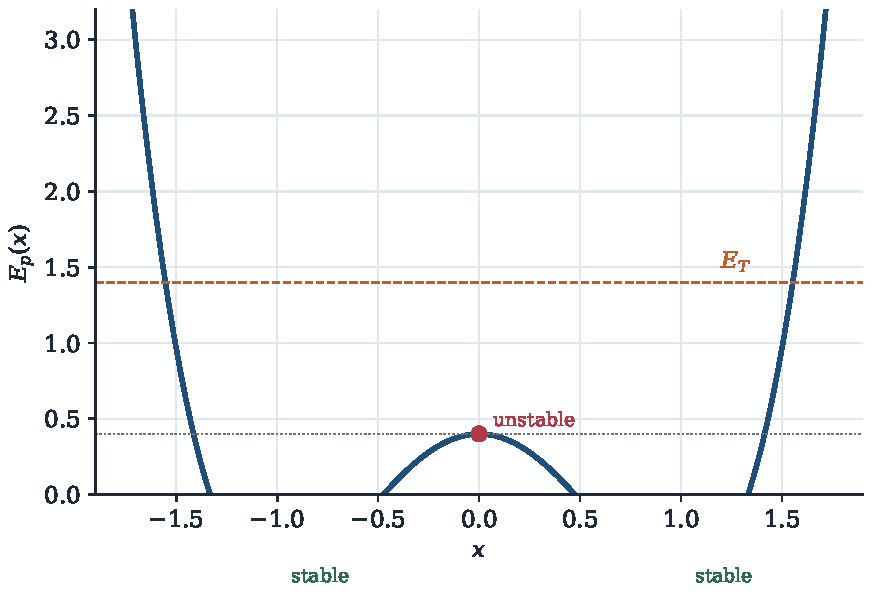
\includegraphics[width=0.74\textwidth]{figures/15_energy_well.pdf}
\caption{One-dimensional potential energy landscape $E_p(x)$. For a particle with mechanical energy $E_m$, the motion is confined to the classically allowed region between the turning points $x_1$ and $x_2$ where $E_p(x) = E_m$. At local minima ($x_0$), equilibrium is stable; at local maxima ($x_{\text{max}}$), equilibrium is unstable.}
\label{fig:energy_well}
\end{figure}

Solving the energy conservation equation for the velocity $\dot{x} = \dd x/\dd t$:
\begin{equation}
\dot{x} = \pm \sqrt{\frac{2}{m}\left( E_m - E_p(x) \right)}.
\end{equation}

\begin{definitionbox}{Classically Allowed Regions and Turning Points}
\begin{itemize}[leftmargin=1.5em,itemsep=3pt]
  \item \textbf{Classically Allowed Region:} The set of coordinates $\{x \in \mathbb{R} \mid E_p(x) \le E_m\}$. The kinetic energy is positive, and the particle moves with real non-zero velocity.
  \item \textbf{Classically Forbidden Region:} The set of coordinates $\{x \in \mathbb{R} \mid E_p(x) > E_m\}$. In classical mechanics, penetration into this region is strictly impossible because it would require imaginary velocity (or negative kinetic energy).
  \item \textbf{Turning Points (Inversion Points):} The spatial boundaries $x_t$ where the mechanical energy line intersects the potential curve:
  \begin{equation}
  E_p(x_t) = E_m \implies v(x_t) = 0.
  \end{equation}
  At a turning point, the particle comes to rest instantaneously, reverses its direction of motion, and accelerates back into the well under the force $F(x_t) = -E_p'(x_t)$.
\end{itemize}
\end{definitionbox}

If the allowed region is a finite interval $[x_1, x_2]$ bounded by two turning points ($E_p(x_1) = E_p(x_2) = E_m$), the particle is trapped in a \textbf{potential well} and executes bounded periodic oscillatory motion. The exact period of oscillation $T$ is given by separating variables $\dd t = \frac{\dd x}{\sqrt{\frac{2}{m}(E_m - E_p(x))}}$:
\begin{equation}
T = 2 \int_{x_1}^{x_2} \frac{\dd x}{\sqrt{\frac{2}{m}\left( E_m - E_p(x) \right)}}.
\end{equation}

\section{Equilibrium Points and Stability Classification}

A material point is in mechanical equilibrium if the net force acting on it vanishes:
\begin{equation}
F(x_0) = 0 \iff \left.\frac{\dd E_p}{\dd x}\right|_{x_0} = 0.
\end{equation}
Thus, \textbf{the points of equilibrium correspond geometrically to the stationary points (horizontal tangents) of the potential energy curve}.

To evaluate the stability of an equilibrium point $x_0$, we perform a Taylor series expansion of the potential energy $E_p(x)$ around $x_0$ for small displacements $\eta \eqdef x - x_0$:
\begin{equation}
E_p(x_0 + \eta) = E_p(x_0) + \underbrace{\left.\frac{\dd E_p}{\dd x}\right|_{x_0}}_{= 0}\eta + \frac{1}{2}\left.\frac{\dd^2 E_p}{\dd x^2}\right|_{x_0}\eta^2 + \frac{1}{6}\left.\frac{\dd^3 E_p}{\dd x^3}\right|_{x_0}\eta^3 + \mathcal{O}(\eta^4).
\end{equation}
Defining the \textbf{effective spring constant}:
\begin{equation}
k_{\text{eff}} \eqdef \left.\frac{\dd^2 E_p}{\dd x^2}\right|_{x_0}.
\end{equation}
The restoring force acting on the displaced particle is:
\begin{equation}
F(\eta) = -\frac{\dd E_p}{\dd\eta} \approx -k_{\text{eff}}\,\eta - \frac{1}{2} E_p'''(x_0)\,\eta^2.
\end{equation}

\begin{lawbox}{Classification of Equilibrium States}
\begin{enumerate}[leftmargin=1.5em,itemsep=4pt]
  \item \textbf{Stable Equilibrium ($k_{\text{eff}} > 0$):}
  The potential energy curve is concave upward ($\frac{\dd^2 E_p}{\dd x^2} > 0$), possessing a \textbf{local minimum} at $x_0$. A positive displacement ($\eta > 0$) induces a negative restoring force ($F < 0$), pulling the particle back toward $x_0$.
  \item \textbf{Unstable Equilibrium ($k_{\text{eff}} < 0$):}
  The potential energy curve is concave downward ($\frac{\dd^2 E_p}{\dd x^2} < 0$), possessing a \textbf{local maximum} at $x_0$. Any infinitesimal displacement ($\eta \neq 0$) produces a repulsive force ($F \approx |k_{\text{eff}}|\eta$) accelerating the particle away from $x_0$ exponentially: $\eta(t) \propto e^{\lambda t}$ with $\lambda = \sqrt{|k_{\text{eff}}|/m}$.
  \item \textbf{Neutral (Indifferent) Equilibrium ($k_{\text{eff}} = 0$):}
  The potential is locally flat to second order. Stability is determined by the first non-vanishing higher derivative $E_p^{(n)}(x_0)$:
  \begin{itemize}[leftmargin=1.2em,itemsep=2pt]
    \item If $n$ is odd, the point is an inflection point and is \emph{unstable}.
    \item If $n$ is even and $E_p^{(n)}(x_0) > 0$, the equilibrium is \emph{stable}.
    \item If $n$ is even and $E_p^{(n)}(x_0) < 0$, the equilibrium is \emph{unstable}.
  \end{itemize}
\end{enumerate}
\end{lawbox}

\begin{figure}[htbp]
\centering
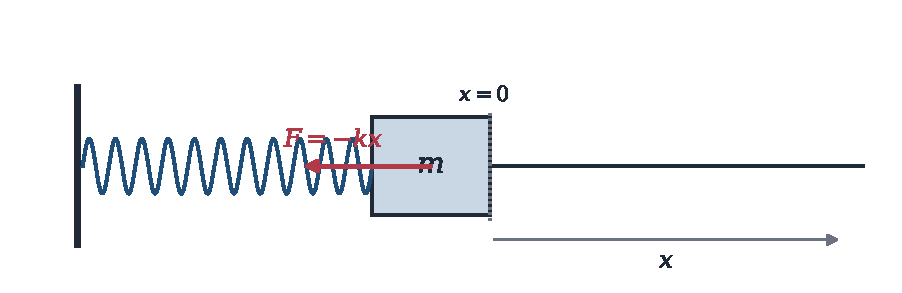
\includegraphics[width=0.62\textwidth]{figures/14_spring_mass.pdf}
\caption{The universal harmonic prototype: a mass-spring system whose quadratic potential $E_p(x) = \frac{1}{2}k x^2$ models the bottom of any generic smooth potential energy well.}
\label{fig:spring_mass}
\end{figure}

\section{The Harmonic Approximation and Small Oscillations}

Near any regular stable equilibrium minimum $x_0$ ($k_{\text{eff}} = E_p''(x_0) > 0$), we truncate the Taylor expansion at quadratic order:
\begin{equation}
E_p(\eta) \approx E_p(x_0) + \frac{1}{2} k_{\text{eff}}\,\eta^2.
\end{equation}
Newton's second law for the displacement $\eta(t) = x(t) - x_0$ yields:
\begin{equation}
m \frac{\dd^2\eta}{\dd t^2} = F(\eta) \approx -k_{\text{eff}}\,\eta \implies \frac{\dd^2\eta}{\dd t^2} + \omega_0^2\,\eta = 0.
\end{equation}

\begin{lawbox}{Universal Frequency of Small Oscillations}
For sufficiently small perturbations about any stable equilibrium point $x_0$, the motion is universally simple harmonic with natural angular frequency:
\begin{equation}
\omega_0 \eqdef \sqrt{\frac{k_{\text{eff}}}{m}} = \sqrt{\frac{1}{m}\left.\frac{\dd^2 E_p}{\dd x^2}\right|_{x_0}}.
\end{equation}
The natural period of small oscillations is:
\begin{equation}
T_0 = \frac{2\pi}{\omega_0} = 2\pi\sqrt{\frac{m}{E_p''(x_0)}}.
\end{equation}
\end{lawbox}

This remarkable theorem implies that \textbf{all physical systems, no matter how complex their underlying microscopic forces, behave as simple harmonic oscillators in the limit of small displacements about a stable equilibrium}.

\section{Comprehensive Worked Examples}

\begin{workedexample}{The Lennard-Jones (6-12) Intermolecular Potential}
The interaction potential between two neutral noble gas atoms (e.g., Argon) separated by a distance $r > 0$ is accurately described by the empirical Lennard-Jones (6-12) potential:
\begin{equation}
V(r) = 4\varepsilon \left[ \left(\frac{\sigma}{r}\right)^{12} - \left(\frac{\sigma}{r}\right)^6 \right],
\end{equation}
where $\varepsilon > 0$ is the depth of the attractive well and $\sigma > 0$ is the distance at which the interatomic potential vanishes ($V(\sigma) = 0$).
\begin{enumerate}[leftmargin=1.4em,itemsep=3pt]
  \item Derive the interatomic interaction force $F(r) = -\frac{\dd V}{\dd r}$ and identify the repulsive and attractive regimes.
  \item Determine the equilibrium separation distance $r_0$ and compute the binding energy $V(r_0)$.
  \item Calculate the effective spring constant $k_{\text{eff}} = V''(r_0)$ and determine the frequency $\omega_0$ of small molecular vibrations for a diatomic molecule of reduced mass $\mu$.
\end{enumerate}

\paragraph{Solution.}
\textbf{1. Interatomic Force:}\\
Differentiating the Lennard-Jones potential with respect to $r$:
\[
F(r) = -\frac{\dd V}{\dd r} = -4\varepsilon \left[ -12\frac{\sigma^{12}}{r^{13}} - \left(-6\frac{\sigma^6}{r^7}\right) \right] = \frac{24\varepsilon}{r}\left[ 2\left(\frac{\sigma}{r}\right)^{12} - \left(\frac{\sigma}{r}\right)^6 \right].
\]
\begin{itemize}[leftmargin=1.5em,itemsep=2pt]
  \item When $r < 2^{1/6}\sigma$, $2(\sigma/r)^{12} > (\sigma/r)^6$, so $F(r) > 0$: the force is strongly \textbf{repulsive}, originating from Pauli exclusion between overlapping electronic clouds.
  \item When $r > 2^{1/6}\sigma$, $2(\sigma/r)^{12} < (\sigma/r)^6$, so $F(r) < 0$: the force is \textbf{attractive}, corresponding to long-range induced dipole-dipole (van der Waals / London dispersion) interactions.
\end{itemize}

\textbf{2. Equilibrium Distance and Well Depth:}\\
Equilibrium occurs where the net force vanishes, $F(r_0) = 0$:
\[
2\left(\frac{\sigma}{r_0}\right)^{12} = \left(\frac{\sigma}{r_0}\right)^6 \implies \left(\frac{\sigma}{r_0}\right)^6 = \frac{1}{2} \implies r_0 = 2^{1/6}\,\sigma \approx 1.12246\,\sigma.
\]
Evaluating the potential at this equilibrium distance:
\[
V(r_0) = 4\varepsilon \left[ \left(\frac{1}{2}\right)^2 - \frac{1}{2} \right] = 4\varepsilon \left( \frac{1}{4} - \frac{1}{2} \right) = 4\varepsilon \left(-\frac{1}{4}\right) = -\varepsilon.
\]
The potential well depth is exactly $-\varepsilon$. A minimum energy $\Delta E = +\varepsilon$ (the dissociation energy) must be supplied to separate the atoms to infinite distance.

\textbf{3. Effective Stiffness and Vibrational Frequency:}\\
Differentiating $F(r)$ to compute the second derivative of the potential:
\[
V''(r) = -\frac{\dd F}{\dd r} = -\frac{\dd}{\dd r}\left( \frac{48\varepsilon \sigma^{12}}{r^{13}} - \frac{24\varepsilon \sigma^6}{r^7} \right) = \frac{48 \times 13\,\varepsilon \sigma^{12}}{r^{14}} - \frac{24 \times 7\,\varepsilon \sigma^6}{r^8}.
\]
Evaluating at $r_0$ where $(\sigma/r_0)^6 = 1/2$ and $(\sigma/r_0)^{12} = 1/4$:
\[
V''(r_0) = \frac{\varepsilon}{r_0^2}\left[ 48 \times 13 \left(\frac{\sigma}{r_0}\right)^{12} - 24 \times 7 \left(\frac{\sigma}{r_0}\right)^6 \right] = \frac{\varepsilon}{r_0^2}\left[ 624\left(\frac{1}{4}\right) - 168\left(\frac{1}{2}\right) \right].
\]
\[
V''(r_0) = \frac{\varepsilon}{r_0^2}\left[ 156 - 84 \right] = \frac{72\,\varepsilon}{r_0^2} = \frac{72\,\varepsilon}{2^{1/3}\sigma^2} \approx \frac{57.14\,\varepsilon}{\sigma^2} > 0.
\]
Since $V''(r_0) > 0$, the equilibrium is strictly stable. The natural vibrational frequency of the diatomic molecule is:
\[
\omega_0 = \sqrt{\frac{k_{\text{eff}}}{\mu}} = \sqrt{\frac{72\varepsilon}{\mu\, r_0^2}} = \frac{6}{r_0}\sqrt{\frac{2\varepsilon}{\mu}},
\]
where $\mu = \frac{m_1 m_2}{m_1 + m_2}$ is the reduced mass of the pair.
\end{workedexample}

\begin{workedexample}{The Quartic Double-Well Potential and Symmetry Breaking}
A particle of mass $m$ moves in a one-dimensional symmetrical quartic potential:
\begin{equation}
E_p(x) = -\frac{1}{2}\alpha\, x^2 + \frac{1}{4}\beta\, x^4, \qquad \alpha > 0,\ \beta > 0.
\end{equation}
\begin{enumerate}[leftmargin=1.4em,itemsep=3pt]
  \item Find all equilibrium positions and classify their stability.
  \item Determine the potential depth at the stable minima and sketch the energy threshold separating oscillatory motion confined to a single well from large-scale oscillations crossing both wells.
  \item Find the frequency $\omega_0$ of small oscillations about the stable minima.
\end{enumerate}

\paragraph{Solution.}
\textbf{1. Equilibrium Points:}\\
The force is $F(x) = -E_p'(x) = \alpha x - \beta x^3 = x(\alpha - \beta x^2)$.
Equilibrium points satisfy $F(x) = 0$:
\[
x_0 = 0, \qquad \text{or} \qquad x_{\pm} = \pm \sqrt{\frac{\alpha}{\beta}}.
\]
To classify their stability, we evaluate the second derivative:
\[
E_p''(x) = -\alpha + 3\beta x^2.
\]
\begin{itemize}[leftmargin=1.5em,itemsep=2pt]
  \item At the origin $x_0 = 0$:
  \[
  E_p''(0) = -\alpha < 0 \implies \textbf{Unstable equilibrium (local maximum)}.
  \]
  \item At the twin equilibria $x_{\pm} = \pm\sqrt{\alpha/\beta}$:
  \[
  E_p''(x_{\pm}) = -\alpha + 3\beta\left(\frac{\alpha}{\beta}\right) = 2\alpha > 0 \implies \textbf{Stable equilibria (twin local minima)}.
  \]
\end{itemize}

\textbf{2. Well Depth and Energy Regimes:}\\
Evaluating the potential at the equilibria:
\[
E_p(0) = 0, \qquad E_p(x_{\pm}) = -\frac{1}{2}\alpha\left(\frac{\alpha}{\beta}\right) + \frac{1}{4}\beta\left(\frac{\alpha}{\beta}\right)^2 = -\frac{\alpha^2}{2\beta} + \frac{\alpha^2}{4\beta} = -\frac{\alpha^2}{4\beta}.
\]
The potential possesses two symmetric minima of depth $-\Delta E = -\frac{\alpha^2}{4\beta}$ separated by a central potential barrier of height $E_p(0) = 0$.
\begin{itemize}[leftmargin=1.5em,itemsep=2pt]
  \item If $-\frac{\alpha^2}{4\beta} < E_m < 0$: the motion is bounded inside either the left well ($x < 0$) or the right well ($x > 0$). The particle cannot cross the barrier at $x = 0$. The reflection symmetry of the system is \emph{spontaneously broken} by the particle's choice of well.
  \item If $E_m = 0$: this is the \textbf{separatrix}. The particle reaches $x = 0$ asymptotically as $t \to \infty$.
  \item If $E_m > 0$: the particle has sufficient energy to surmount the central barrier, executing wide oscillations enclosing both minima between turning points $x = \pm x_t$.
\end{itemize}

\textbf{3. Frequency of Small Oscillations:}\\
Near either stable minimum $x = x_{\pm}$, the effective stiffness is $k_{\text{eff}} = E_p''(x_{\pm}) = 2\alpha$.
The natural angular frequency of small oscillations is:
\[
\omega_0 = \sqrt{\frac{k_{\text{eff}}}{m}} = \sqrt{\frac{2\alpha}{m}}.
\]
This model represents the classic Landau theory of second-order phase transitions, spontaneous symmetry breaking in quantum field theory (the Higgs mechanism), and the inversion vibration of the ammonia molecule ($\mathrm{NH}_3$).
\end{workedexample}

\begin{workedexample}{Vertical Hydrodynamic Stability and Bobbing of a Floating Spar}
A solid vertical cylindrical spar buoy of uniform mass $m$, total length $H$, and constant cross-sectional area $S$ floats vertically in a calm sea of water of density $\rho_w$. The density of the spar is $\rho_s < \rho_w$.
\begin{enumerate}[leftmargin=1.4em,itemsep=3pt]
  \item Determine the equilibrium submerged draft $h_0$.
  \item Express the total potential energy $E_p(z)$ as a function of the vertical displacement $z$ from equilibrium.
  \item Show that the vertical equilibrium is unconditionally stable and compute the period of small vertical heaving oscillations.
\end{enumerate}

\paragraph{Solution.}
\textbf{1. Equilibrium Draft:}\\
Let $h_0$ be the submerged depth in static equilibrium. The buoyant force (Archimedes' principle) equals the weight of displaced fluid:
\[
F_{\text{buoyant}} = \rho_w S h_0\, g.
\]
The gravitational weight of the spar is $P = m g = \rho_s S H\, g$.
Equating buoyancy to weight:
\[
\rho_w S h_0 g = \rho_s S H g \implies h_0 = \frac{\rho_s}{\rho_w} H.
\]

\textbf{2. Potential Energy Function:}\\
Let $z$ be the upward vertical displacement from the equilibrium draft $h_0$. When the cylinder is displaced upward by $z$, its submerged depth becomes $h = h_0 - z$.
The net vertical restoring force acting on the spar is:
\[
F_z(z) = F_{\text{buoyant}} - P = \rho_w S (h_0 - z) g - mg = \rho_w S h_0 g - \rho_w S g z - mg.
\]
Since $\rho_w S h_0 g = mg$:
\[
F_z(z) = -\rho_w S g\, z.
\]
The potential energy associated with this linear restoring force (taking $E_p(0) = 0$ at equilibrium) is:
\[
E_p(z) = -\int_0^z F_z(z')\,\dd z' = \int_0^z \rho_w S g\, z'\,\dd z' = \frac{1}{2} \rho_w S g\, z^2.
\]

\textbf{3. Stability and Heaving Period:}\\
Evaluating the second derivative of the potential energy:
\[
k_{\text{eff}} = \left.\frac{\dd^2 E_p}{\dd z^2}\right|_{z = 0} = \rho_w S g > 0.
\]
Because $\rho_w S g > 0$ strictly, the vertical equilibrium is unconditionally stable.
The differential equation of motion is:
\[
m \ddot{z} + \rho_w S g z = 0 \implies \ddot{z} + \omega_0^2 z = 0, \qquad \omega_0 = \sqrt{\frac{\rho_w S g}{m}}.
\]
Substituting $m = \rho_s S H = \rho_w S h_0$:
\[
\omega_0 = \sqrt{\frac{\rho_w S g}{\rho_w S h_0}} = \sqrt{\frac{g}{h_0}}.
\]
The natural period of vertical heaving oscillations is:
\[
T_0 = \frac{2\pi}{\omega_0} = 2\pi\sqrt{\frac{h_0}{g}}.
\]
This expression is formally identical to the period of a simple pendulum of length $L = h_0$, demonstrating the mathematical unity of classical mechanics.
\end{workedexample}

\chapter{Linear Oscillations: Free, Damped, and Forced Resonance}
\label{ch:oscillations}

\begin{chapterintro}
\textbf{Chapter Objectives:} In this chapter, we develop the comprehensive mathematical theory of linear oscillations. You will master the free harmonic oscillator and its phase-space geometry; analyze viscous damping across underdamped, critically damped, and overdamped regimes; quantify energy dissipation via the logarithmic decrement $\delta$ and quality factor $Q$; derive the exact amplitude and phase response of sinusoidally driven oscillators; uncover the distinction between amplitude resonance and velocity resonance; and calculate the normal modes and beat phenomena of coupled oscillators.
\end{chapterintro}

\section{The Free Undamped Harmonic Oscillator}

Any mechanical system possessing a stable equilibrium state obeys, for sufficiently small perturbations, the canonical homogeneous differential equation:
\begin{equation}
\frac{\dd^2 x}{\dd t^2} + \omega_0^2\, x = 0, \qquad \omega_0 \eqdef \sqrt{\frac{k}{m}}.
\end{equation}
The general real solution may be expressed in three equivalent forms:
\begin{align}
x(t) &= A \cos(\omega_0 t + \phi) \\
     &= C_1 \cos(\omega_0 t) + C_2 \sin(\omega_0 t) \\
     &= \operatorname{Re}\left( \underline{X}_0 e^{i\omega_0 t} \right), \quad \underline{X}_0 = A e^{i\phi} \in \mathbb{C}.
\end{align}

\begin{figure}[htbp]
\centering
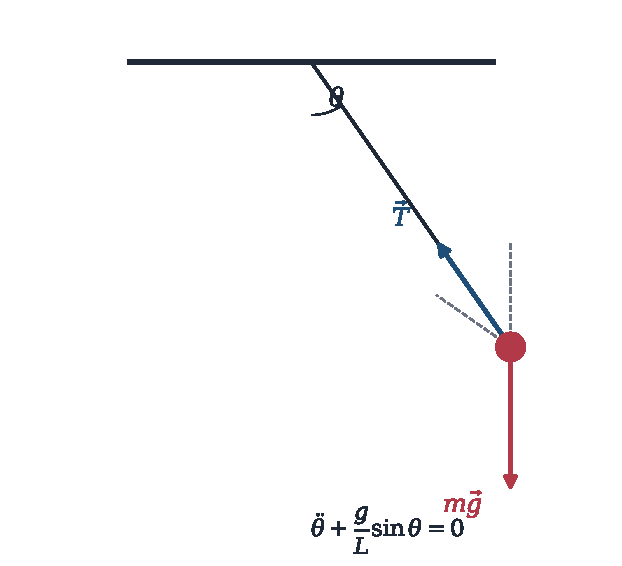
\includegraphics[width=0.72\textwidth]{figures/20_pendulum.pdf}
\caption{The simple gravity pendulum of length $L$. For small angular displacements ($\sin\theta \approx \theta$), the motion is strictly harmonic with angular frequency $\omega_0 = \sqrt{g/L}$. The phase portrait shows concentric elliptical trajectories around the stable center $(0,0)$ and the homoclinic separatrix passing through the unstable inverted equilibrium $(\pm\pi, 0)$.}
\label{fig:pendulum}
\end{figure}

Differentiating with respect to time yields the velocity:
\begin{equation}
v(t) = \dot{x}(t) = -\omega_0 A \sin(\omega_0 t + \phi) = \omega_0 A \cos\left(\omega_0 t + \phi + \frac{\pi}{2}\right).
\end{equation}
\emph{Key kinematic property:} The velocity leads the displacement by a phase quadrature of $\pi/2\ \mathrm{rad}$ ($90^\circ$).

\subsection{Energy and Phase Space Trajectory}

The instantaneous kinetic and potential energies are:
\begin{equation}
E_k(t) = \frac{1}{2}m v(t)^2 = \frac{1}{2}m \omega_0^2 A^2 \sin^2(\omega_0 t + \phi),
\end{equation}
\begin{equation}
E_p(t) = \frac{1}{2}k x(t)^2 = \frac{1}{2}m \omega_0^2 A^2 \cos^2(\omega_0 t + \phi).
\end{equation}
Adding these expressions confirms rigorous energy conservation at every instant:
\begin{equation}
E_m = E_k(t) + E_p(t) = \frac{1}{2}m \omega_0^2 A^2 = \frac{1}{2}k A^2 = \text{constant}.
\end{equation}
Averaging over a full cycle $T_0 = 2\pi/\omega_0$, using $\langle \sin^2 \rangle = \langle \cos^2 \rangle = \frac{1}{2}$:
\begin{equation}
\langle E_k \rangle = \langle E_p \rangle = \frac{1}{4} m \omega_0^2 A^2 = \frac{1}{2} E_m.
\end{equation}
In phase space with coordinates $(x, \dot{x}/\omega_0)$, the trajectory is a circle of radius $A$; in standard phase space $(x, v)$, it is an ellipse of semi-axes $A$ and $\omega_0 A$:
\begin{equation}
\frac{x^2}{A^2} + \frac{v^2}{\omega_0^2 A^2} = 1.
\end{equation}

\begin{historicalbox}{Christiaan Huygens and the Isochronous Pendulum}
\begin{minipage}{0.28\textwidth}
\centering
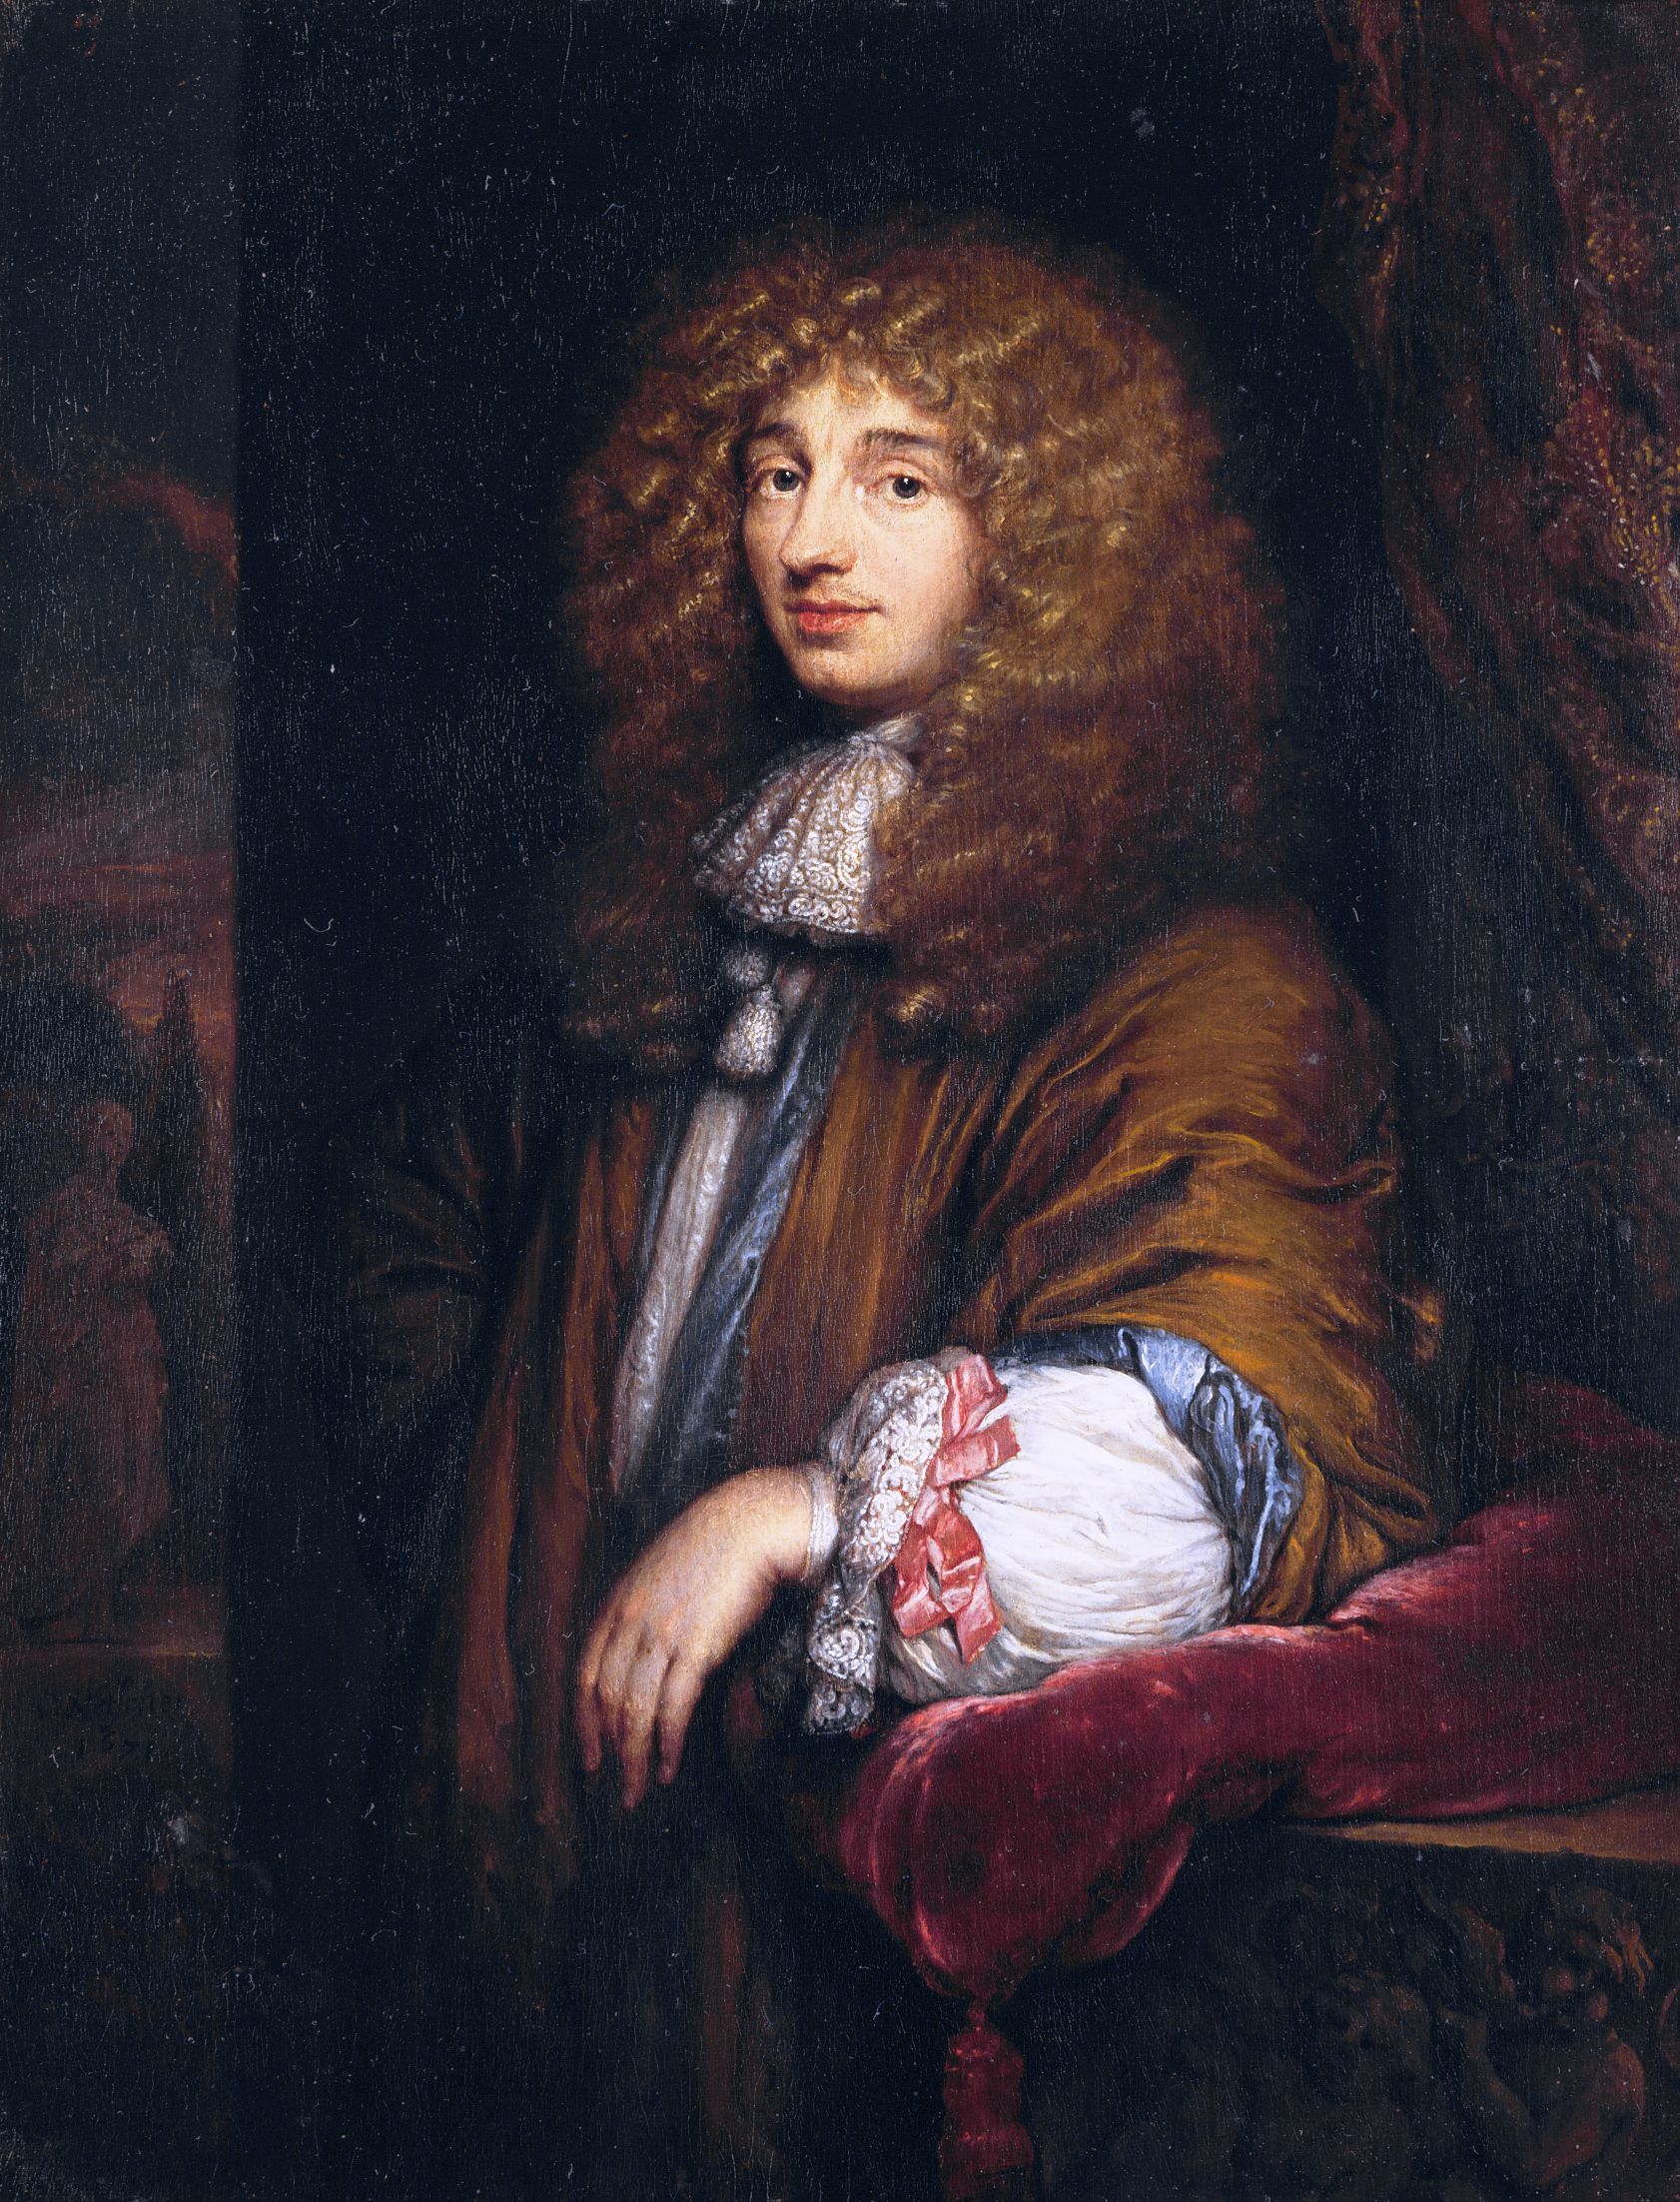
\includegraphics[width=0.92\textwidth]{images/huygens.jpg}
\captionof{figure}{Christiaan Huygens (1629--1695), portrait by Caspar Netscher (1671, Haags Historisch Museum).}
\end{minipage}\hfill
\begin{minipage}{0.68\textwidth}
In 1656, Dutch mathematician and physicist Christiaan Huygens invented the pendulum clock, dramatically increasing timekeeping accuracy from 15 minutes per day to under 15 seconds. In his 1673 masterpiece \emph{Horologium Oscillatorium}, Huygens proved mathematically that while a circular pendulum is only approximately isochronous for tiny angles ($\sin\theta \approx \theta$), a pendulum whose bob is guided between cycloidal cheeks executes \textbf{strictly isochronous oscillations} of period $T = 2\pi\sqrt{L/g}$ regardless of amplitude.

Huygens also made the first recorded observation of \textbf{synchronization} in 1665: two pendulum clocks mounted to the same wooden beam gradually locked into antiphase alignment through minuscule vibrations transmitted through the structure.
\end{minipage}
\end{historicalbox}

\section{Damped Oscillations (Viscous Resistance)}

Real mechanical systems inevitably encounter fluid resistance or internal friction. Modeling the dissipative force as linear viscous damping $\vec{F}_d = -\lambda \vec{v}$ ($\lambda > 0$), Newton's second law reads:
\begin{equation}
m \ddot{x} = -k x - \lambda \dot{x} \implies \ddot{x} + 2\gamma \dot{x} + \omega_0^2 x = 0,
\end{equation}
where we introduce the \textbf{damping parameter} $\gamma$ and the dimensionless \textbf{damping ratio} $\zeta$:
\begin{equation}
\gamma \eqdef \frac{\lambda}{2m}, \qquad \zeta \eqdef \frac{\gamma}{\omega_0} = \frac{\lambda}{2\sqrt{k m}}.
\end{equation}
Seeking solutions of the form $x(t) = e^{r t}$ leads to the characteristic algebraic equation:
\begin{equation}
r^2 + 2\gamma r + \omega_0^2 = 0 \implies r_{1,2} = -\gamma \pm \sqrt{\gamma^2 - \omega_0^2}.
\end{equation}

\begin{figure}[htbp]
\centering
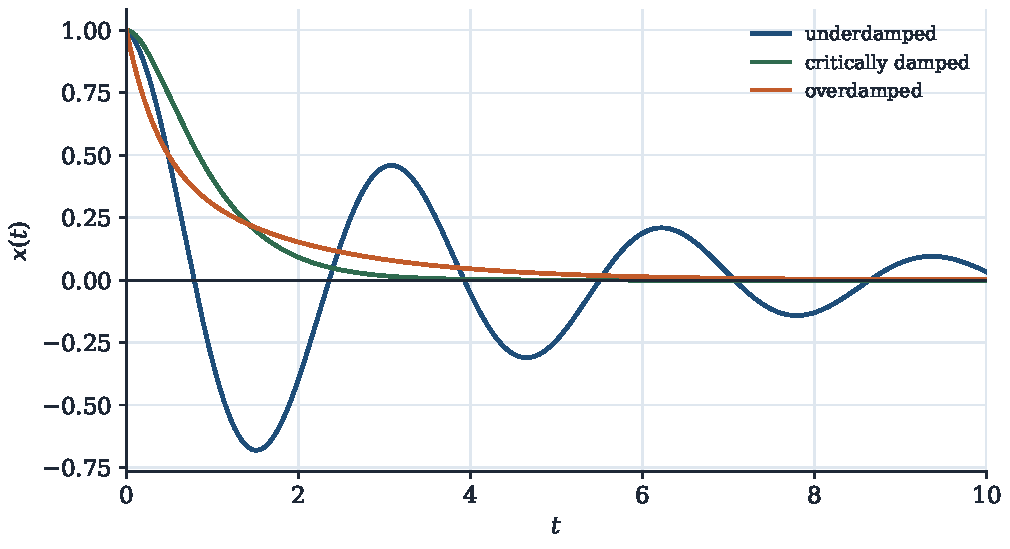
\includegraphics[width=0.74\textwidth]{figures/16_damped_oscillations.pdf}
\caption{Evolution of a damped oscillator for identical initial displacement $x(0) = x_0, \dot{x}(0) = 0$: (1) underdamped oscillatory decay ($\zeta < 1$, blue); (2) critically damped non-oscillatory return ($\zeta = 1$, green); (3) overdamped sluggish relaxation ($\zeta > 1$, red).}
\label{fig:damped_oscillations}
\end{figure}

The nature of the motion depends fundamentally on the sign of the discriminant $\Delta = \gamma^2 - \omega_0^2$:

\subsection{1. Underdamped Regime ($\gamma < \omega_0$, $\zeta < 1$)}
The roots are complex conjugates $r_{1,2} = -\gamma \pm i \omega_d$, where the \textbf{pseudofrequency} is:
\begin{equation}
\omega_d \eqdef \sqrt{\omega_0^2 - \gamma^2} = \omega_0 \sqrt{1 - \zeta^2} < \omega_0.
\end{equation}
The general real solution describes pseudo-periodic oscillations decaying exponentially within an envelope:
\begin{equation}
x(t) = A_0 e^{-\gamma t} \cos(\omega_d t + \phi).
\end{equation}
The \textbf{pseudoperiod} is $T_d = \frac{2\pi}{\omega_d} = \frac{2\pi}{\sqrt{\omega_0^2 - \gamma^2}} > T_0$. Damping systematically lengthens the period of oscillation.

\begin{definitionbox}{Logarithmic Decrement and Quality Factor}
The \textbf{logarithmic decrement} $\delta$ measures the rate of amplitude decay between successive peaks separated by one pseudoperiod $T_d$:
\begin{equation}
\delta \eqdef \ln\left( \frac{x(t)}{x(t + T_d)} \right) = \ln\left( \frac{e^{-\gamma t}}{e^{-\gamma(t + T_d)}} \right) = \gamma T_d = \frac{2\pi \gamma}{\omega_d} = \frac{2\pi \zeta}{\sqrt{1 - \zeta^2}}.
\end{equation}
The dimensionless \textbf{Quality Factor} $Q$ quantifies the sharpness of the oscillator's energy retention:
\begin{equation}
Q \eqdef \frac{\omega_0}{2\gamma} = \frac{1}{2\zeta} = \frac{\sqrt{km}}{\lambda} \approx \frac{\pi}{\delta} \quad (\text{for } Q \gg 1).
\end{equation}
The fractional energy loss per oscillation cycle is related to $Q$ by:
\begin{equation}
\frac{|\Delta E_m|}{E_m} \approx \frac{2\pi}{Q}.
\end{equation}
\end{definitionbox}

\subsection{2. Critically Damped Regime ($\gamma = \omega_0$, $\zeta = 1$)}
The characteristic equation has a degenerate double real root $r = -\gamma$. The general solution is:
\begin{equation}
x(t) = (C_1 + C_2 t) e^{-\gamma t}.
\end{equation}
\emph{Engineering Significance:} Critical damping provides the \textbf{fastest possible return to equilibrium without oscillation or overshoot}. It is the design target for automotive shock absorbers, analog galvanometer meters, and seismic dampers.

\subsection{3. Overdamped Regime ($\gamma > \omega_0$, $\zeta > 1$)}
The roots are distinct, negative real numbers $r_{1,2} = -\gamma \pm \sqrt{\gamma^2 - \omega_0^2} < 0$. The solution is:
\begin{equation}
x(t) = C_1 e^{-(\gamma - \sqrt{\gamma^2 - \omega_0^2})t} + C_2 e^{-(\gamma + \sqrt{\gamma^2 - \omega_0^2})t}.
\end{equation}
The motion is non-oscillatory and exhibits sluggish exponential creeping dominated by the slow decay rate $\lambda_{\text{slow}} = \gamma - \sqrt{\gamma^2 - \omega_0^2}$.

\section{Forced Oscillations and Resonance}

Subjecting the damped oscillator to an external harmonic driving force $F(t) = F_0 \cos(\Omega t)$:
\begin{equation}
\ddot{x} + 2\gamma \dot{x} + \omega_0^2 x = \frac{F_0}{m} \cos(\Omega t).
\end{equation}
The general solution is the superposition of the transient complementary solution $x_h(t)$ (which decays exponentially to zero) and the permanent \textbf{steady-state response} $x_p(t)$:
\begin{equation}
x_p(t) = X_0(\Omega) \cos(\Omega t - \varphi(\Omega)).
\end{equation}

\subsection{Complex Impedance Derivation}
Representing the driving force as $\underline{F}(t) = F_0 e^{i\Omega t}$ and the response as $\underline{x}(t) = \underline{X}_0 e^{i\Omega t}$:
\[
(-\Omega^2 + 2i\gamma\Omega + \omega_0^2) \underline{X}_0 = \frac{F_0}{m} \implies \underline{X}_0 = \frac{F_0 / m}{(\omega_0^2 - \Omega^2) + 2i\gamma\Omega}.
\]
Taking the modulus and argument:

\begin{lawbox}{Resonance Amplitude and Phase Lag}
The steady-state oscillation amplitude is:
\begin{equation}
X_0(\Omega) = \frac{F_0 / m}{\sqrt{(\omega_0^2 - \Omega^2)^2 + 4\gamma^2\Omega^2}} = \frac{F_0 / k}{\sqrt{\left(1 - \frac{\Omega^2}{\omega_0^2}\right)^2 + \frac{1}{Q^2}\left(\frac{\Omega}{\omega_0}\right)^2}}.
\end{equation}
The phase lag $\varphi(\Omega) \in [0, \pi]$ by which displacement trails the force is:
\begin{equation}
\tan\varphi(\Omega) = \frac{2\gamma\Omega}{\omega_0^2 - \Omega^2}.
\end{equation}
\begin{itemize}[leftmargin=1.5em,itemsep=2pt]
  \item At low frequencies ($\Omega \ll \omega_0$): $X_0 \to F_0/k$ (quasi-static response, in phase: $\varphi \to 0$).
  \item At exact tuning ($\Omega = \omega_0$): $\varphi = \pi/2$ (quadrature). The velocity is strictly in phase with the force, maximizing instantaneous power transfer!
  \item At high frequencies ($\Omega \gg \omega_0$): $X_0 \to \frac{F_0}{m\Omega^2} \to 0$ (inertia-dominated, antiphase: $\varphi \to \pi$).
\end{itemize}
\end{lawbox}

\begin{definitionbox}{Amplitude Resonance vs Velocity Resonance}
\begin{itemize}[leftmargin=1.5em,itemsep=3pt]
  \item \textbf{Amplitude Resonance:} The frequency $\Omega_r$ that maximizes $X_0(\Omega)$ minimizes the denominator $f(u) = (\omega_0^2 - u)^2 + 4\gamma^2 u$ (where $u = \Omega^2$):
  \begin{equation}
  \Omega_r = \sqrt{\omega_0^2 - 2\gamma^2} = \omega_0 \sqrt{1 - \frac{1}{2Q^2}}.
  \end{equation}
  Amplitude resonance exists if and only if $\gamma < \omega_0/\sqrt{2}$ ($Q > 1/\sqrt{2} \approx 0.707$).
  At this peak, the maximum amplitude is:
  \begin{equation}
  X_{\max} = X_0(\Omega_r) = \frac{F_0 / m}{2\gamma\sqrt{\omega_0^2 - \gamma^2}} \approx Q \left(\frac{F_0}{k}\right) \quad (\text{for } Q \gg 1).
  \end{equation}
  \item \textbf{Velocity Resonance:} The velocity amplitude $V_0(\Omega) = \Omega X_0(\Omega) = \frac{F_0/m}{\sqrt{(\omega_0^2/\Omega - \Omega)^2 + 4\gamma^2}}$ attains its global maximum \textbf{strictly at $\Omega = \omega_0$} for any level of damping.
  \item \textbf{Half-Power Resonance Bandwidth:} The full width at half-maximum power is:
  \begin{equation}
  \Delta\Omega = 2\gamma = \frac{\omega_0}{Q}.
  \end{equation}
\end{itemize}
\end{definitionbox}

\section{Comprehensive Worked Examples}

\begin{workedexample}{Experimental Determination of Damping and Quality Factor}
A harmonic mass-spring oscillator has inertial mass $m = 0.50\ \mathrm{kg}$ and spring stiffness $k = 200\ \mathrm{N\cdot m^{-1}}$. When set into motion in a viscous liquid, a high-speed camera records that the displacement amplitude decreases by a factor of $3.0$ over $6$ complete oscillation cycles.
\begin{enumerate}[leftmargin=1.4em,itemsep=3pt]
  \item Compute the logarithmic decrement $\delta$ and the damping parameter $\gamma$.
  \item Calculate the viscous damping coefficient $\lambda$ and the Quality Factor $Q$.
  \item Determine the percentage difference between the pseudofrequency $\omega_d$ and the undamped natural frequency $\omega_0$.
\end{enumerate}

\paragraph{Solution.}
\textbf{1. Logarithmic Decrement and Damping Parameter:}\\
The amplitude after $N = 6$ complete periods satisfies:
\[
\frac{A(t)}{A(t + N T_d)} = e^{N \gamma T_d} = 3.0 \implies N \gamma T_d = \ln(3.0) \approx 1.0986.
\]
The logarithmic decrement per single period is:
\[
\delta = \gamma T_d = \frac{\ln(3.0)}{N} = \frac{1.0986}{6} \approx 0.1831.
\]
The undamped angular frequency is:
\[
\omega_0 = \sqrt{\frac{k}{m}} = \sqrt{\frac{200}{0.50}} = \sqrt{400} = 20.0\ \mathrm{rad\cdot s^{-1}}.
\]
Since $\delta = \frac{2\pi \gamma}{\omega_d} = \frac{2\pi \zeta}{\sqrt{1 - \zeta^2}}$, we invert for the damping ratio $\zeta$:
\[
\frac{\zeta^2}{1 - \zeta^2} = \left(\frac{\delta}{2\pi}\right)^2 = \left(\frac{0.1831}{6.2832}\right)^2 = (0.02914)^2 \approx 8.492\times 10^{-4}.
\]
Because $\zeta \ll 1$, to high accuracy $\zeta \approx 0.02914$.
The damping parameter $\gamma$ is:
\[
\gamma = \zeta \omega_0 = (0.02914)(20.0) \approx 0.5828\ \mathrm{s^{-1}}.
\]

\textbf{2. Viscous Coefficient and Quality Factor:}\\
The fluid resistance coefficient $\lambda$ is:
\[
\lambda = 2m\gamma = 2(0.50\ \mathrm{kg})(0.5828\ \mathrm{s^{-1}}) \approx 0.583\ \mathrm{kg\cdot s^{-1}} = 0.583\ \mathrm{N\cdot s\cdot m^{-1}}.
\]
The Quality Factor $Q$ is:
\[
Q = \frac{\omega_0}{2\gamma} = \frac{20.0}{2(0.5828)} = \frac{20.0}{1.1656} \approx 17.16 \approx \frac{\pi}{\delta} = \frac{3.1416}{0.1831} \approx 17.16.
\]

\textbf{3. Frequency Shift:}\\
The pseudofrequency is:
\[
\omega_d = \omega_0\sqrt{1 - \zeta^2} = 20.0\sqrt{1 - (0.02914)^2} = 20.0\sqrt{1 - 0.000849} \approx 20.0(1 - 0.000425) = 19.9915\ \mathrm{rad\cdot s^{-1}}.
\]
The relative frequency shift is:
\[
\frac{\omega_0 - \omega_d}{\omega_0} \approx \frac{1}{2}\zeta^2 = \frac{1}{2}(0.02914)^2 \approx 0.042\% \quad (\text{less than } 1 \text{ part in } 2300!).
\]
Even with substantial amplitude attenuation ($3\times$ reduction in 6 cycles), the frequency of oscillation remains virtually indistinguishable from the undamped resonance.
\end{workedexample}

\begin{workedexample}{Seismic Base Excitation and Vibration Isolation}
A sensitive scientific instrument of mass $m$ is mounted on an elastic suspension of total stiffness $k$ and viscous damper $\lambda$ anchored to a laboratory foundation. During an earthquake, the foundation undergoes horizontal harmonic displacement $y(t) = Y_0 \cos(\Omega t)$.
\begin{enumerate}[leftmargin=1.4em,itemsep=3pt]
  \item Derive the differential equation of motion for the absolute coordinate $x(t)$ of the instrument.
  \item Determine the transmissibility ratio $T_r \eqdef X_0 / Y_0$ of displacement amplitude transmitted to the instrument as a function of the frequency ratio $\beta \eqdef \Omega/\omega_0$ and damping ratio $\zeta$.
  \item Prove that effective vibration isolation ($T_r < 1$) is achieved if and only if $\beta > \sqrt{2}$.
\end{enumerate}

\paragraph{Solution.}
\textbf{1. Differential Equation of Motion:}\\
The spring force depends on relative elongation $\Delta l = x - y$, and the damper force depends on relative velocity $\dot{x} - \dot{y}$:
\[
m \ddot{x} = -k(x - y) - \lambda(\dot{x} - \dot{y}) \implies m\ddot{x} + \lambda\dot{x} + kx = \lambda\dot{y} + ky.
\]
Dividing by $m$ and using $\omega_0^2 = k/m$ and $2\gamma = \lambda/m = 2\zeta\omega_0$:
\[
\ddot{x} + 2\zeta\omega_0 \dot{x} + \omega_0^2 x = 2\zeta\omega_0 \dot{y} + \omega_0^2 y.
\]

\textbf{2. Transmissibility Ratio:}\\
Using complex representation $\underline{y}(t) = Y_0 e^{i\Omega t}$, so $\dot{\underline{y}}(t) = i\Omega Y_0 e^{i\Omega t}$. The driving terms are:
\[
\omega_0^2 \underline{y} + 2\zeta\omega_0 \dot{\underline{y}} = (\omega_0^2 + 2i\zeta\omega_0\Omega) Y_0 e^{i\Omega t}.
\]
Assuming steady-state response $\underline{x}(t) = \underline{X}_0 e^{i\Omega t}$:
\[
\left( -\Omega^2 + 2i\zeta\omega_0\Omega + \omega_0^2 \right) \underline{X}_0 = (\omega_0^2 + 2i\zeta\omega_0\Omega) Y_0.
\]
Dividing by $\omega_0^2$ and introducing $\beta = \Omega/\omega_0$:
\[
\underline{X}_0 = Y_0 \frac{1 + 2i\zeta\beta}{(1 - \beta^2) + 2i\zeta\beta}.
\]
Taking the absolute modulus of the numerator and denominator:
\[
T_r \eqdef \frac{X_0}{Y_0} = \sqrt{\frac{1 + (2\zeta\beta)^2}{(1 - \beta^2)^2 + (2\zeta\beta)^2}}.
\]

\textbf{3. Criterion for Vibration Isolation:}\\
For the suspension to isolate the instrument from floor vibrations, the transmitted amplitude must be strictly smaller than the ground amplitude, $T_r < 1$:
\[
\frac{1 + (2\zeta\beta)^2}{(1 - \beta^2)^2 + (2\zeta\beta)^2} < 1 \iff 1 + (2\zeta\beta)^2 < (1 - \beta^2)^2 + (2\zeta\beta)^2.
\]
Subtracting $(2\zeta\beta)^2$ from both sides:
\[
1 < (1 - \beta^2)^2 \iff (1 - \beta^2)^2 - 1 > 0 \iff \beta^2(\beta^2 - 2) > 0.
\]
Since $\beta > 0$, this inequality is satisfied if and only if:
\[
\beta^2 - 2 > 0 \implies \beta > \sqrt{2} \implies \Omega > \sqrt{2}\,\omega_0.
\]
\emph{Profound Engineering Conclusion:}
\begin{itemize}[leftmargin=1.5em,itemsep=2pt]
  \item For $\Omega < \sqrt{2}\omega_0$, $T_r > 1$: the suspension \textbf{amplifies} foundation vibrations.
  \item At $\Omega = \sqrt{2}\omega_0$, $T_r = 1$ identically, regardless of the value of damping $\zeta$.
  \item To isolate high-frequency equipment or buildings against seismic ground waves, engineers design very ``soft'' suspensions with very low natural frequency $\omega_0$ so that the operating or earthquake frequency satisfies $\Omega \gg \sqrt{2}\omega_0$.
\end{itemize}
\end{workedexample}

\begin{workedexample}{Coupled Oscillators, Normal Modes, and the Phenomenon of Beats}
Two identical carts of mass $m_1 = m_2 = m$ slide along a frictionless horizontal track. Each cart is anchored to an adjacent wall by an outer spring of stiffness $k$, and the two carts are coupled to each other by a central spring of stiffness $k_c$.
\begin{enumerate}[leftmargin=1.4em,itemsep=3pt]
  \item Write Newton's second law for both carts in matrix form $M \ddot{\vec{X}} + K \vec{X} = \vzero$.
  \item Solve the secular eigenvalue equation to find the two normal mode frequencies $\omega_1$ and $\omega_2$ and their corresponding modal eigenvectors.
  \item Cart 1 is initially displaced by $x_1(0) = a$ while cart 2 is held at $x_2(0) = 0$, and both are released from rest. Show that the subsequent motion exhibits beats and compute the beat period $T_{\text{beat}}$.
\end{enumerate}

\paragraph{Solution.}
\textbf{1. Coupled Differential Equations of Motion:}\\
Let $x_1$ and $x_2$ denote the displacements of cart 1 and cart 2 from their respective equilibrium positions.
\begin{align*}
m \ddot{x}_1 &= -k x_1 - k_c (x_1 - x_2) = -(k + k_c) x_1 + k_c x_2, \\
m \ddot{x}_2 &= -k x_2 - k_c (x_2 - x_1) = k_c x_1 - (k + k_c) x_2.
\end{align*}
In matrix notation with $\vec{X} = \begin{pmatrix} x_1 \\ x_2 \end{pmatrix}$:
\[
\begin{pmatrix} m & 0 \\ 0 & m \end{pmatrix} \begin{pmatrix} \ddot{x}_1 \\ \ddot{x}_2 \end{pmatrix} + \begin{pmatrix} k + k_c & -k_c \\ -k_c & k + k_c \end{pmatrix} \begin{pmatrix} x_1 \\ x_2 \end{pmatrix} = \begin{pmatrix} 0 \\ 0 \end{pmatrix}.
\]

\textbf{2. Normal Modes and Eigenvalues:}\\
Seeking harmonic normal mode solutions $\vec{X}(t) = \vec{A} \cos(\omega t)$ leads to the eigenvalue problem:
\[
\det\left( K - \omega^2 M \right) = \det\begin{pmatrix} (k + k_c) - m\omega^2 & -k_c \\ -k_c & (k + k_c) - m\omega^2 \end{pmatrix} = 0.
\]
This yields:
\[
\left[(k + k_c) - m\omega^2\right]^2 - k_c^2 = 0 \implies (k + k_c) - m\omega^2 = \pm k_c.
\]
We obtain two distinct normal mode frequencies:
\begin{itemize}[leftmargin=1.5em,itemsep=3pt]
  \item \textbf{Mode 1 (Symmetric / In-Phase Mode):} Choosing $+k_c$:
  \[
  m\omega_1^2 = (k + k_c) - k_c = k \implies \omega_1 = \sqrt{\frac{k}{m}}.
  \]
  The modal eigenvector satisfies $-k_c A_{11} + k_c A_{12} = 0 \implies A_{11} = A_{12}$.
  \[
  \vec{A}^{(1)} = \frac{1}{\sqrt{2}}\begin{pmatrix} 1 \\ 1 \end{pmatrix}.
  \]
  In this mode, both carts move in perfect synchronization ($x_1(t) = x_2(t)$). The central spring length remains constant ($\Delta l_c = x_1 - x_2 = 0$); it exerts zero force, oscillating at the uncoupled frequency $\sqrt{k/m}$.
  \item \textbf{Mode 2 (Antisymmetric / Out-of-Phase Mode):} Choosing $-k_c$:
  \[
  m\omega_2^2 = (k + k_c) + k_c = k + 2k_c \implies \omega_2 = \sqrt{\frac{k + 2k_c}{m}} > \omega_1.
  \]
  The modal eigenvector satisfies $k_c A_{21} + k_c A_{22} = 0 \implies A_{21} = -A_{22}$.
  \[
  \vec{A}^{(2)} = \frac{1}{\sqrt{2}}\begin{pmatrix} 1 \\ -1 \end{pmatrix}.
  \]
  In this mode, the carts move in exact opposition ($x_1(t) = -x_2(t)$). The central spring is compressed/extended twice as much, providing extra stiffness and raising the frequency.
\end{itemize}

\textbf{3. Superposition and Beat Phenomenon:}\\
The general solution is a linear superposition of the two normal modes:
\[
x_1(t) = C_1 \cos(\omega_1 t + \phi_1) + C_2 \cos(\omega_2 t + \phi_2),
\]
\[
x_2(t) = C_1 \cos(\omega_1 t + \phi_1) - C_2 \cos(\omega_2 t + \phi_2).
\]
Applying initial conditions: $x_1(0) = a, x_2(0) = 0, \dot{x}_1(0) = 0, \dot{x}_2(0) = 0$:
\[
C_1 + C_2 = a, \qquad C_1 - C_2 = 0 \implies C_1 = C_2 = \frac{a}{2}, \quad \phi_1 = \phi_2 = 0.
\]
The exact trajectories of the two carts are:
\begin{align*}
x_1(t) &= \frac{a}{2}\left( \cos(\omega_1 t) + \cos(\omega_2 t) \right) = a \cos\left(\frac{\omega_2 - \omega_1}{2} t\right) \cos\left(\frac{\omega_2 + \omega_1}{2} t\right), \\
x_2(t) &= \frac{a}{2}\left( \cos(\omega_1 t) - \cos(\omega_2 t) \right) = a \sin\left(\frac{\omega_2 - \omega_1}{2} t\right) \sin\left(\frac{\omega_2 + \omega_1}{2} t\right).
\end{align*}
For weak coupling ($k_c \ll k$), $\omega_2 \approx \omega_1$, defining the mean carrier frequency $\bar{\omega} = \frac{\omega_1 + \omega_2}{2}$ and the modulation frequency $\omega_{\text{mod}} = \frac{\omega_2 - \omega_1}{2} \ll \bar{\omega}$.

The energy sloshes periodically back and forth between cart 1 and cart 2. When cart 1 is at maximum amplitude, cart 2 is momentarily stationary, and vice versa.
The beat period (time between successive amplitude nulls for cart 1) is:
\[
T_{\text{beat}} = \frac{2\pi}{\omega_2 - \omega_1} \approx \frac{2\pi}{\sqrt{\frac{k+2k_c}{m}} - \sqrt{\frac{k}{m}}} \approx \frac{2\pi}{\sqrt{\frac{k}{m}}\left(1 + \frac{k_c}{k} - 1\right)} = \frac{2\pi}{\omega_0} \frac{k}{k_c}.
\]
\end{workedexample}


\part{Central Forces, Celestial Mechanics, and Systems}

\chapter{Central Forces, Gravitation, and Celestial Mechanics}
\label{ch:central_forces}

\begin{chapterintro}
\textbf{Chapter Objectives:} In this chapter, we develop the complete analytical theory of central conservative forces. You will discover the fundamental consequences of angular momentum conservation and Kepler's law of areas; construct the one-dimensional effective radial potential $U_{\text{eff}}(r)$ with its centrifugal barrier; derive Binet's kinematic and dynamic formulas; solve the Kepler-Newton gravitational problem; prove Kepler's three laws; calculate interplanetary orbital transfers using the vis-viva equation; and analyze planetary gravitational assists and Rutherford scattering.
\end{chapterintro}

\section{Properties of Central Force Fields}

\begin{definitionbox}{Central Force Field}
A force field $\vec{F}(\vec{r})$ acting on a material point $M$ is said to be \textbf{central} with respect to a fixed origin $O$ if the line of action of the force passes through $O$ at every instant:
\begin{equation}
\vec{F}(\vec{r}) = F(r)\,\ur = F(r)\,\frac{\vec{r}}{r}, \qquad r = \norm{\vec{r}}.
\end{equation}
The force is said to be \textbf{attractive} if $F(r) < 0$ and \textbf{repulsive} if $F(r) > 0$.
\end{definitionbox}

\begin{figure}[htbp]
\centering
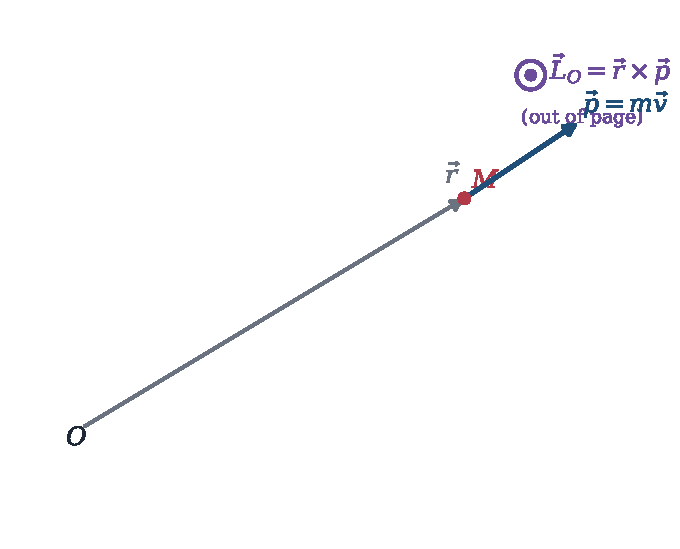
\includegraphics[width=0.74\textwidth]{figures/22_angular_momentum.pdf}
\caption{Conservation of angular momentum in central motion. The moment of a central force $\vec{F} = F(r)\ur$ with respect to center $O$ vanishes identically ($\vec{\mathcal{M}}_O = \vec{r}\times\vec{F} = \vzero$), freezing the angular momentum vector $\vec{L}_O = \vec{r}\times\vec{p}$ in magnitude and spatial orientation.}
\label{fig:angular_momentum}
\end{figure}

\begin{lawbox}{The Fundamental Theorem of Central Motion}
For any particle moving under a central force field centered at $O$, the angular momentum $\vec{L}_O$ with respect to $O$ is an invariant of motion:
\begin{equation}
\frac{\dd\vec{L}_O}{\dd t} = \vec{\mathcal{M}}_O(\vec{F}) = \vec{r} \times \vec{F} = \vec{r} \times (F(r)\ur) = \vzero \implies \vec{L}_O = \vec{r} \times m\vec{v} = \text{constant vector}.
\end{equation}
\textbf{Profound Geometrical Consequence (Planarity):}
Since $\vec{L}_O$ is a constant vector orthogonal to both $\vec{r}(t)$ and $\vec{v}(t)$ at every instant:
\begin{equation}
\vec{r}(t) \cdot \vec{L}_O \equiv 0.
\end{equation}
\textbf{The trajectory of a particle subject to a central force is strictly confined to a fixed two-dimensional plane} passing through the force center $O$ and perpendicular to $\vec{L}_O$.
\end{lawbox}

\section{Kepler's Second Law (Law of Areas) and Areal Velocity}

Adopting plane polar coordinates $(r, \theta)$ in the orbital plane with origin at $O$:
\[
\vec{r} = r\,\ur, \qquad \vec{v} = \dot{r}\,\ur + r\dot{\theta}\,\ut.
\]
The angular momentum vector is:
\begin{equation}
\vec{L}_O = \vec{r} \times m\vec{v} = (r\,\ur) \times m(\dot{r}\,\ur + r\dot{\theta}\,\ut) = m r^2 \dot{\theta}\,\khat \eqdef L\,\khat.
\end{equation}
Since $\vec{L}_O$ is constant, the scalar magnitude $L = m r^2 \dot{\theta}$ is strictly conserved:
\begin{equation}
C \eqdef r^2 \dot{\theta} = \frac{L}{m} = \text{constant of areas}.
\end{equation}

\begin{figure}[htbp]
\centering
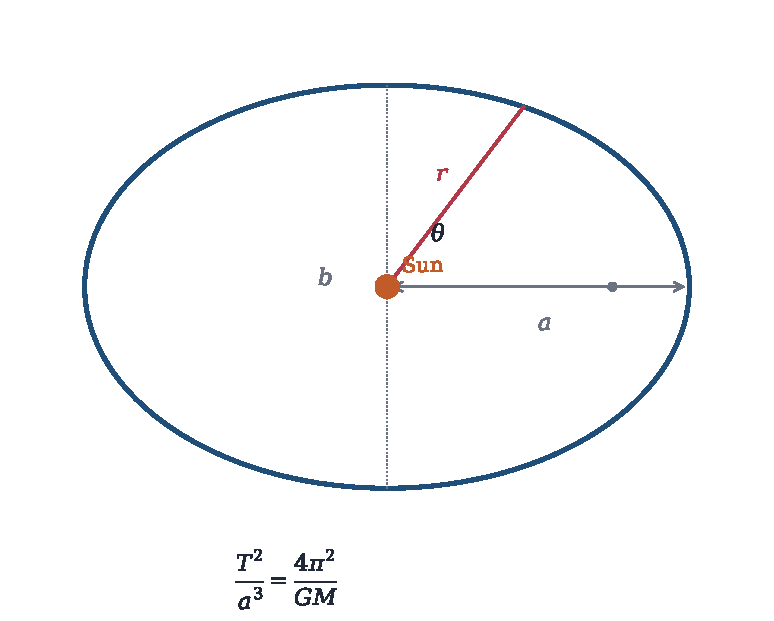
\includegraphics[width=0.74\textwidth]{figures/17_kepler.pdf}
\caption{Kepler's Second Law: equal areas in equal times. An orbiting body sweeps out equal planar sectors $\Delta A_1 = \Delta A_2$ in equal time intervals $\Delta t$, traveling fastest at perihelion ($r_{\min}$) and slowest at aphelion ($r_{\max}$).}
\label{fig:kepler}
\end{figure}

During an infinitesimal time $\dd t$, the position vector $\vec{r}$ rotates through angle $\dd\theta$, sweeping out an elementary triangular sector of area:
\begin{equation}
\dd A = \frac{1}{2} \norm{\vec{r} \times \dd\vec{r}} = \frac{1}{2} r (r\,\dd\theta) = \frac{1}{2} r^2 \dd\theta.
\end{equation}
Dividing by $\dd t$ yields the \textbf{areal velocity}:
\begin{equation}
\frac{\dd A}{\dd t} = \frac{1}{2} r^2 \dot{\theta} = \frac{C}{2} = \frac{L}{2m} = \text{constant}.
\end{equation}

\begin{lawbox}{Kepler's Second Law (Law of Areas)}
The radius vector joining the force center to the particle sweeps out equal planar areas in equal intervals of time throughout the entire motion:
\begin{equation}
\Delta A = \frac{L}{2m} \Delta t.
\end{equation}
As a direct consequence, the linear speed is inversely proportional to the instantaneous distance to the center: at perihelion ($r_p$), speed is maximum ($v_p = C/r_p$); at aphelion ($r_a$), speed is minimum ($v_a = C/r_a$).
\end{lawbox}

\begin{historicalbox}{Johannes Kepler and the New Astronomy}
\begin{minipage}{0.28\textwidth}
\centering
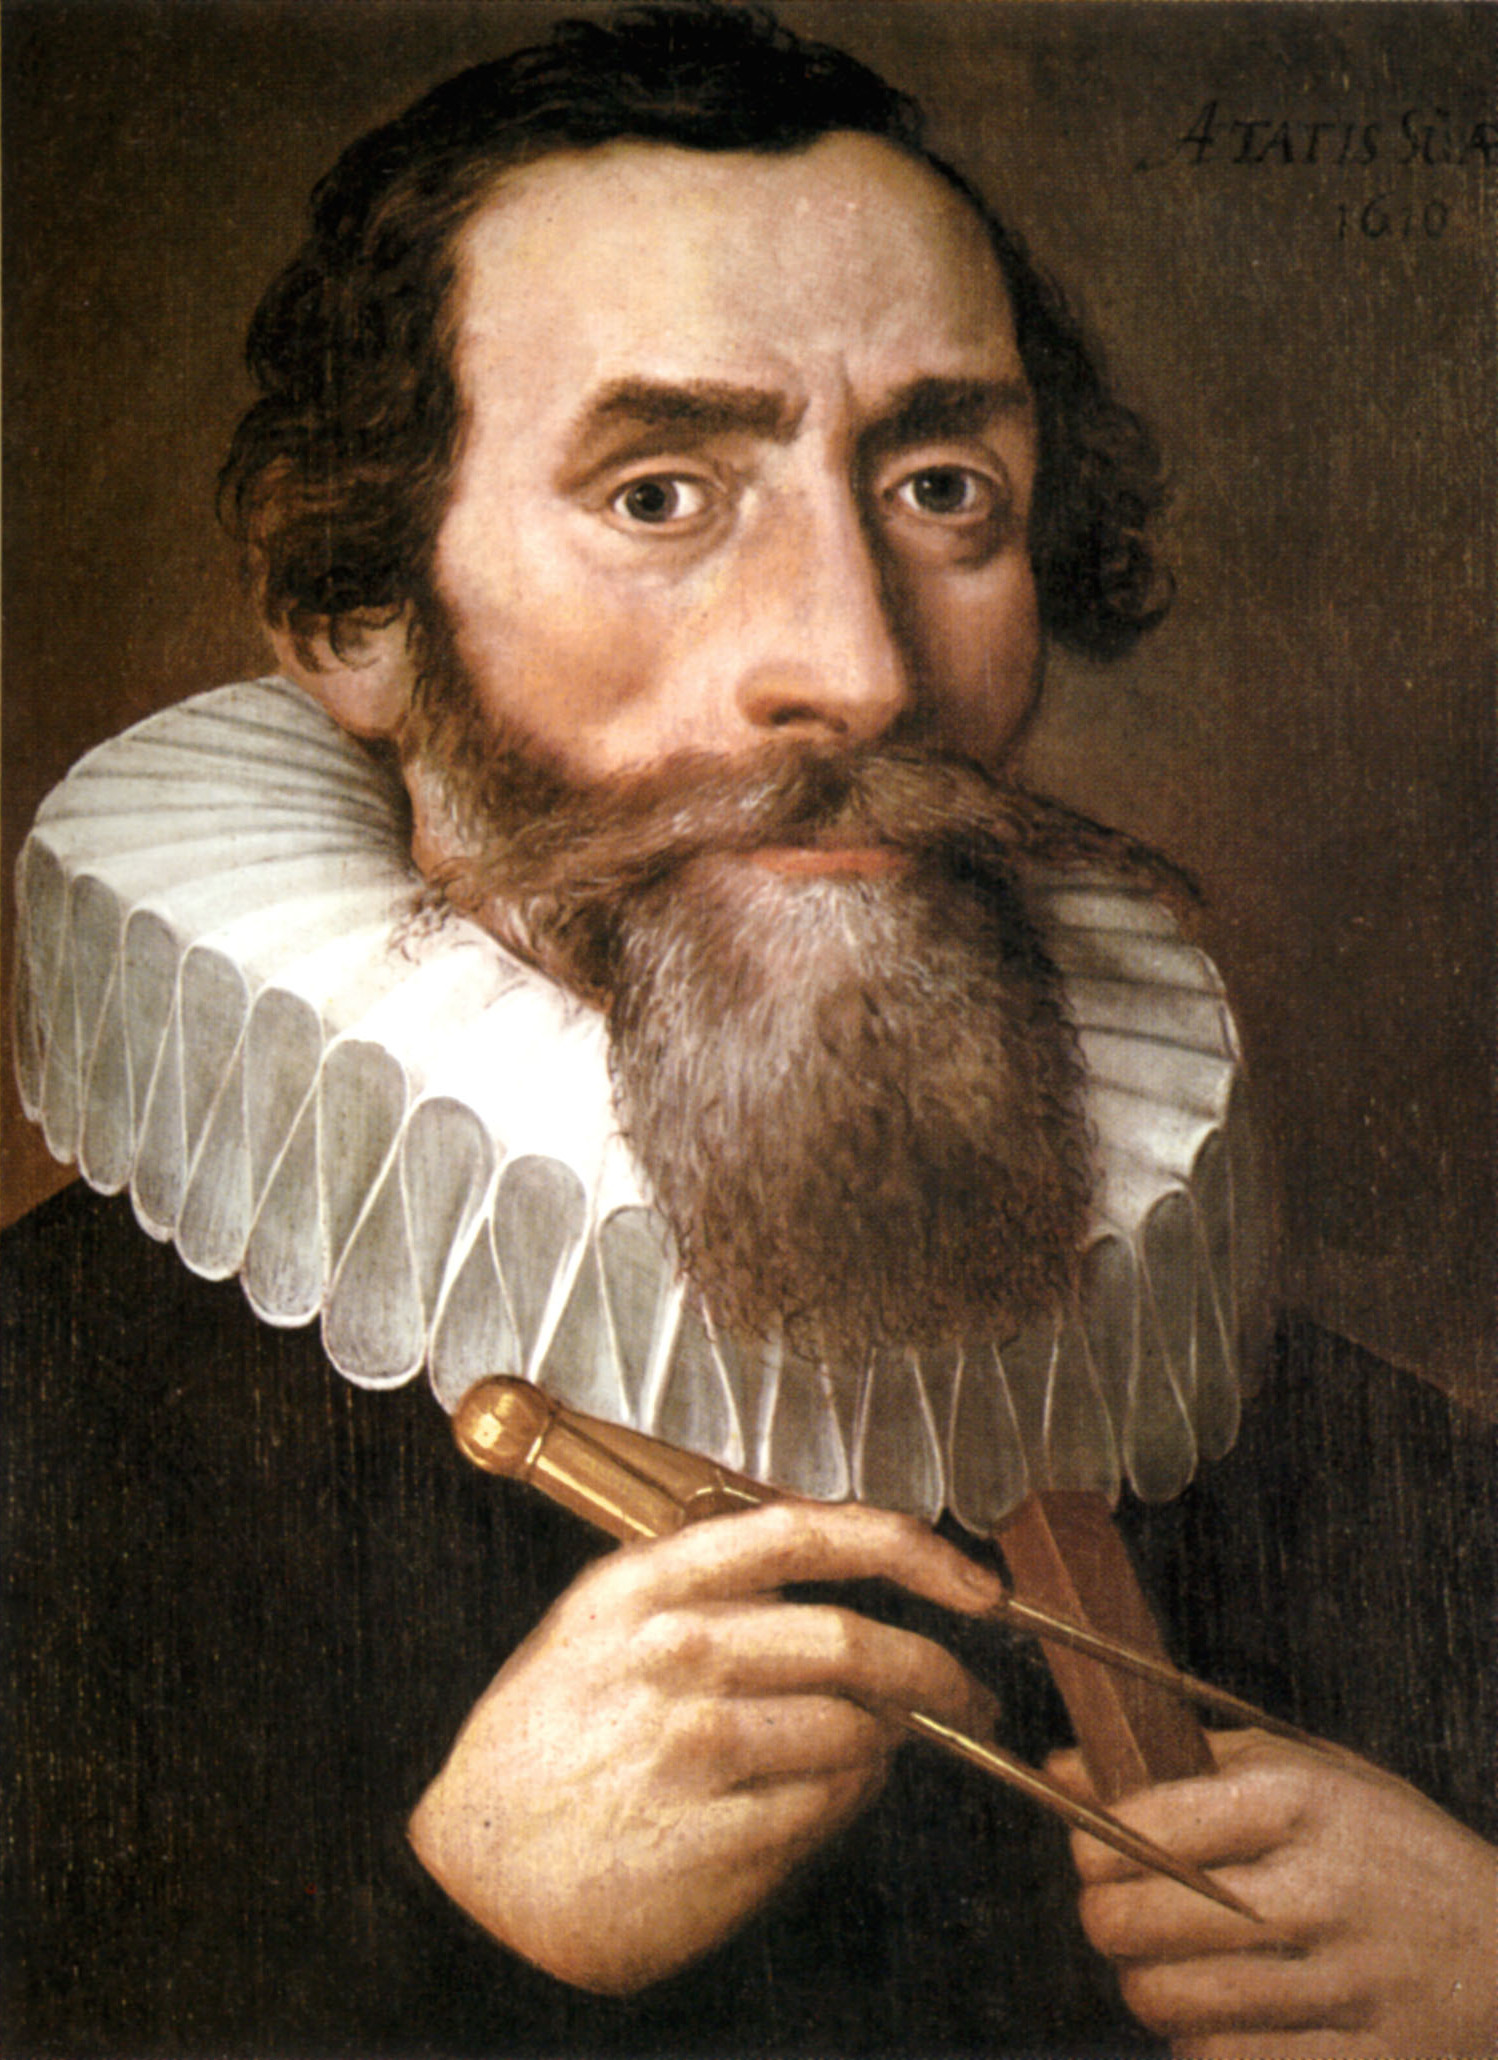
\includegraphics[width=0.92\textwidth]{images/kepler.jpg}
\captionof{figure}{Johannes Kepler (1571--1630), contemporary copper engraving (1610).}
\end{minipage}\hfill
\begin{minipage}{0.68\textwidth}
Working as imperial mathematician to Holy Roman Emperor Rudolf II in Prague, Johannes Kepler inherited decades of ultra-precise naked-eye planetary observations recorded by Tycho Brahe. 

Focusing on the stubborn 8-arcminute discrepancy in the orbit of Mars that could not be reconciled with circular epicycles, Kepler made the revolutionary conceptual leap in \emph{Astronomia Nova} (1609) that planetary orbits are not circles, but \textbf{ellipses with the Sun situated at one focus}. In \emph{Harmonices Mundi} (1619), he unveiled his Third Law, linking orbital periods to semi-major axes ($T^2 \propto a^3$), providing the decisive empirical foundation that led Isaac Newton to the inverse-square law of universal gravitation.
\end{minipage}
\end{historicalbox}

\section{The One-Dimensional Effective Radial Potential}

Because any central force is conservative ($\vec{\nabla}\times(F(r)\ur) = \vzero$), there exists a scalar potential $V(r)$ such that $F(r) = -\frac{\dd V}{\dd r}$.
The total mechanical energy in polar coordinates is:
\begin{equation}
E_m = \frac{1}{2}m v^2 + V(r) = \frac{1}{2}m(\dot{r}^2 + r^2\dot{\theta}^2) + V(r).
\end{equation}
Substituting $\dot{\theta} = \frac{L}{m r^2}$:
\begin{equation}
E_m = \frac{1}{2}m \dot{r}^2 + \frac{L^2}{2m r^2} + V(r) = \frac{1}{2}m \dot{r}^2 + U_{\text{eff}}(r).
\end{equation}

\begin{definitionbox}{Effective Potential Energy}
The two-dimensional central motion is mathematically equivalent to the one-dimensional motion of a fictitious particle of mass $m$ moving in the \textbf{effective radial potential}:
\begin{equation}
U_{\text{eff}}(r) \eqdef V(r) + \frac{L^2}{2m r^2}.
\end{equation}
The term $\frac{L^2}{2m r^2} > 0$ is the \textbf{centrifugal potential barrier}, which acts as a repulsive core preventing any particle with non-zero angular momentum ($L \neq 0$) from collapsing into the origin.
\end{definitionbox}

\section{Binet's Formulas for Trajectory Calculation}

Jacques Philippe Marie Binet (1835) introduced the reciprocal radial variable:
\begin{equation}
u(\theta) \eqdef \frac{1}{r(\theta)}.
\end{equation}
Using the chain rule $\frac{\dd}{\dd t} = \dot{\theta} \frac{\dd}{\dd\theta} = C u^2 \frac{\dd}{\dd\theta}$, the radial position is $r = 1/u$, and the radial velocity is:
\begin{equation}
\dot{r} = \frac{\dd}{\dd t}\left(\frac{1}{u}\right) = -\frac{1}{u^2}\dot{u} = -\frac{1}{u^2} (C u^2) \frac{\dd u}{\dd\theta} = -C \frac{\dd u}{\dd\theta}.
\end{equation}

\begin{lawbox}{Binet's Formulas}
\begin{enumerate}[leftmargin=1.5em,itemsep=3pt]
  \item \textbf{Binet's Kinematic Velocity Formula:}
  \begin{equation}
  v^2 = \dot{r}^2 + r^2\dot{\theta}^2 = C^2 \left[ u^2 + \left(\frac{\dd u}{\dd\theta}\right)^2 \right].
  \end{equation}
  \item \textbf{Binet's Dynamic Acceleration Formula:}
  Differentiating $\dot{r}$ with respect to time and computing radial acceleration $a_r = \ddot{r} - r\dot{\theta}^2$:
  \begin{equation}
  a_r = -C^2 u^2 \left( \frac{\dd^2 u}{\dd\theta^2} + u \right) = \frac{F(1/u)}{m}.
  \end{equation}
\end{enumerate}
\end{lawbox}

\section{The Kepler-Newton Gravitational Problem}

For Newtonian gravitation, the interaction between a central mass $M$ and a satellite mass $m \ll M$ is:
\begin{equation}
\vec{F} = -\frac{G M m}{r^2}\,\ur = -k u^2\,\ur, \qquad k \eqdef G M m.
\end{equation}
Substituting $F(1/u) = -k u^2$ into Binet's dynamic equation:
\[
-C^2 u^2 \left( \frac{\dd^2 u}{\dd\theta^2} + u \right) = -\frac{k u^2}{m} \implies \frac{\dd^2 u}{\dd\theta^2} + u = \frac{k}{m C^2}.
\]
Defining the geometric parameter $p \eqdef \frac{m C^2}{k} = \frac{L^2}{m k}$, known as the \textbf{semi-latus rectum}:
\begin{equation}
\frac{\dd^2 u}{\dd\theta^2} + u = \frac{1}{p}.
\end{equation}
This is the elementary harmonic oscillator differential equation shifted by the constant $1/p$. Its general solution is:
\begin{equation}
u(\theta) = \frac{1}{p}\left[ 1 + e \cos(\theta - \theta_0) \right].
\end{equation}
Choosing the polar axis $\theta = 0$ at periapsis ($\theta_0 = 0$):

\begin{lawbox}{The Conic Equation of Keplerian Orbits}
The trajectory $r(\theta) = 1/u(\theta)$ is a conic section with the gravitational center at one focus:
\begin{equation}
r(\theta) = \frac{p}{1 + e \cos\theta},
\end{equation}
where $e \ge 0$ is the orbital \textbf{eccentricity}, uniquely determined by the mechanical energy $E_m$ and angular momentum $L$:
\begin{equation}
e = \sqrt{1 + \frac{2 E_m L^2}{m k^2}} = \sqrt{1 + \frac{2 E_m C^2 m}{k^2}}.
\end{equation}
\end{lawbox}

\begin{table}[htbp]
\centering
\renewcommand{\arraystretch}{1.35}
\begin{tabular}{@{}llll@{}}
\toprule
\textbf{Energy $E_m$} & \textbf{Eccentricity $e$} & \textbf{Conic Geometry} & \textbf{Physical State} \\
\midrule
$E_m = E_{\min} = -\frac{m k^2}{2 L^2}$ & $e = 0$ & Circle ($r = p = \text{const}$) & Bound periodic orbit \\
$E_{\min} < E_m < 0$ & $0 < e < 1$ & Ellipse ($a = \frac{p}{1-e^2}$) & Bound periodic orbit (Planets, Moons) \\
$E_m = 0$ & $e = 1$ & Parabola ($r_p = p/2$) & Marginally escape threshold \\
$E_m > 0$ & $e > 1$ & Hyperbola ($a = \frac{p}{e^2-1}$) & Unbound flyby trajectory (Comets, Oumuamua) \\
\bottomrule
\end{tabular}
\caption{Classification of Keplerian conic trajectories by energy and eccentricity.}
\label{tab:kepler_conics}
\end{table}

\subsection{Kepler's Third Law and the Vis-Viva Equation}

For an elliptical orbit of semi-major axis $a$ and semi-minor axis $b = a\sqrt{1-e^2}$:
\begin{itemize}[leftmargin=1.5em,itemsep=3pt]
  \item The total orbital area is $A = \pi a b$.
  \item By the law of areas, $\Delta A = \frac{C}{2} T \implies \pi a b = \frac{C}{2} T$.
  \item Since $p = a(1-e^2) = \frac{b^2}{a}$ and $p = \frac{m C^2}{k} = \frac{C^2}{G M}$:
  \[
  C = \sqrt{G M p} = \sqrt{G M \frac{b^2}{a}} = \frac{b}{\sqrt{a}}\sqrt{G M}.
  \]
  \item Squaring the period relation:
  \begin{equation}
  T^2 = \frac{4\pi^2 a^2 b^2}{C^2} = \frac{4\pi^2 a^2 b^2}{(b^2/a) G M} \implies \frac{T^2}{a^3} = \frac{4\pi^2}{G M}.
  \end{equation}
\end{itemize}

\begin{lawbox}{Kepler's Third Law}
The square of the orbital period $T$ of a planet is directly proportional to the cube of the semi-major axis $a$ of its elliptical orbit:
\begin{equation}
\frac{T^2}{a^3} = \frac{4\pi^2}{G(M + m)} \approx \frac{4\pi^2}{G M_\odot}.
\end{equation}
\end{lawbox}

\begin{lawbox}{The Vis-Viva Equation}
For any Keplerian orbit around a central mass $M$, the speed $v(r)$ at distance $r$ is:
\begin{equation}
v^2(r) = G M \left( \frac{2}{r} - \frac{1}{a} \right),
\end{equation}
where $a > 0$ for an ellipse, $a \to \infty$ for a parabola ($v^2 = 2GM/r$), and $a < 0$ for a hyperbola.
\end{lawbox}

\section{Comprehensive Worked Examples}

\begin{workedexample}{The Hohmann Interplanetary Transfer Orbit}
A robotic spacecraft in a circular Low Earth Parking Orbit (LEO) of radius $r_1 = 1.000\ \mathrm{AU} = 1.496\times 10^{11}\ \mathrm{m}$ is to be sent to Mars, whose orbit is modeled as circular and coplanar with radius $r_2 = 1.524\ \mathrm{AU} = 2.280\times 10^{11}\ \mathrm{m}$. Heliocentric gravitation is $G M_\odot = 1.327\times 10^{20}\ \mathrm{m^3\cdot s^{-2}}$.
\begin{enumerate}[leftmargin=1.4em,itemsep=3pt]
  \item Calculate the semi-major axis $a_t$ and the flight duration $\Delta t_{\text{trans}}$ of the elliptical Hohmann transfer orbit.
  \item Compute the orbital speeds $v_1$ (Earth) and $v_2$ (Mars), and determine the injection burn velocity increment $\Delta v_1$ required at perihelion.
  \item Determine the arrival velocity increment $\Delta v_2$ required at aphelion to circularize into Mars's orbit.
\end{enumerate}

\paragraph{Solution.}
\textbf{1. Semi-Major Axis and Transfer Time:}\\
The Hohmann transfer orbit is an ellipse whose perihelion is at Earth ($r_p = r_1$) and whose aphelion is at Mars ($r_a = r_2$). The major axis is the sum:
\[
2a_t = r_1 + r_2 \implies a_t = \frac{r_1 + r_2}{2} = \frac{1.000 + 1.524}{2} = 1.262\ \mathrm{AU} = 1.888\times 10^{11}\ \mathrm{m}.
\]
By Kepler's Third Law, the period of the full transfer ellipse is:
\[
T_t = 1\ \mathrm{yr} \times \left(\frac{a_t}{1\ \mathrm{AU}}\right)^{3/2} = (1.262)^{3/2} \approx 1.4177\ \mathrm{years} \approx 517.8\ \mathrm{days}.
\]
Because the spacecraft traverses exactly half of the ellipse (from perihelion to aphelion), the one-way transit time is:
\[
\Delta t_{\text{trans}} = \frac{1}{2} T_t = \frac{517.8}{2} \approx 258.9\ \mathrm{days} \approx 8.5\ \mathrm{months}.
\]

\textbf{2. Heliocentric Speeds and Injection Burn $\Delta v_1$:}\\
Earth's circular orbital speed is:
\[
v_1 = \sqrt{\frac{G M_\odot}{r_1}} = \sqrt{\frac{1.327\times 10^{20}}{1.496\times 10^{11}}} \approx 29\,780\ \mathrm{m\cdot s^{-1}} \approx 29.78\ \mathrm{km\cdot s^{-1}}.
\]
Mars's circular orbital speed is:
\[
v_2 = \sqrt{\frac{G M_\odot}{r_2}} = \sqrt{\frac{1.327\times 10^{20}}{2.280\times 10^{11}}} \approx 24\,120\ \mathrm{m\cdot s^{-1}} \approx 24.12\ \mathrm{km\cdot s^{-1}}.
\]
Using the vis-viva equation $v^2 = G M_\odot(2/r - 1/a)$, the speed on the transfer ellipse at perihelion ($r = r_1$) is:
\[
v_{t,1} = \sqrt{G M_\odot\left(\frac{2}{r_1} - \frac{1}{a_t}\right)} = \sqrt{1.327\times 10^{20}\left( \frac{2}{1.496\times 10^{11}} - \frac{1}{1.888\times 10^{11}} \right)}.
\]
\[
v_{t,1} = \sqrt{1.327\times 10^{20}(1.3369\times 10^{-11} - 0.5297\times 10^{-11})} = \sqrt{1.071\times 10^9} \approx 32\,730\ \mathrm{m\cdot s^{-1}} \approx 32.73\ \mathrm{km\cdot s^{-1}}.
\]
The required injection boost relative to Earth's heliocentric velocity is:
\[
\Delta v_1 = v_{t,1} - v_1 = 32.73 - 29.78 = 2.95\ \mathrm{km\cdot s^{-1}}.
\]

\textbf{3. Arrival Burn $\Delta v_2$ at Mars:}\\
The speed on the transfer ellipse at aphelion ($r = r_2$) is:
\[
v_{t,2} = \sqrt{G M_\odot\left(\frac{2}{r_2} - \frac{1}{a_t}\right)} = \sqrt{1.327\times 10^{20}\left( \frac{2}{2.280\times 10^{11}} - \frac{1}{1.888\times 10^{11}} \right)}.
\]
\[
v_{t,2} = \sqrt{1.327\times 10^{20}(0.8772\times 10^{-11} - 0.5297\times 10^{-11})} = \sqrt{4.611\times 10^8} \approx 21\,470\ \mathrm{m\cdot s^{-1}} \approx 21.47\ \mathrm{km\cdot s^{-1}}.
\]
To match Mars's circular speed $v_2 = 24.12\ \mathrm{km/s}$, the spacecraft must fire thrusters forward to gain speed:
\[
\Delta v_2 = v_2 - v_{t,2} = 24.12 - 21.47 = 2.65\ \mathrm{km\cdot s^{-1}}.
\]
The total mission delta-v budget is $\Delta v_{\text{total}} = \Delta v_1 + \Delta v_2 = 2.95 + 2.65 = 5.60\ \mathrm{km\cdot s^{-1}}$.
\end{workedexample}

\begin{workedexample}{Planetary Gravity Assist (The Gravitational Slingshot)}
A scientific space probe of mass $m$ encounters Jupiter (mass $M_J \gg m$) on an interplanetary trajectory. In the heliocentric frame $\mathcal{R}_{\odot}$, Jupiter moves with orbital velocity $\vec{V}_J = V_J\,\jhat$ ($V_J \approx 13.0\ \mathrm{km\cdot s^{-1}}$). The probe approaches Jupiter along the $-\jhat$ direction with asymptotic speed $v_0 = 10.0\ \mathrm{km\cdot s^{-1}}$, so $\vec{v}_{\text{in}} = -v_0\,\jhat$.
\begin{enumerate}[leftmargin=1.4em,itemsep=3pt]
  \item Determine the approach speed $u_\infty$ in the rest frame of Jupiter $\mathcal{R}_J$.
  \item The hyperbolic trajectory swings around Jupiter such that its exit velocity is turned by an angle $\delta = 180^\circ$ (a head-on retrograde slingshot). Compute the final heliocentric velocity $\vec{v}_{\text{out}}$ and the kinetic energy gained by the probe.
  \item Explain the source of the mechanical energy gained by the probe.
\end{enumerate}

\paragraph{Solution.}
\textbf{1. Approach Velocity in Jupiter's Rest Frame:}\\
Using the Galilean velocity transformation $\vec{u} = \vec{v} - \vec{V}_J$:
\[
\vec{u}_{\text{in}} = \vec{v}_{\text{in}} - \vec{V}_J = -v_0\,\jhat - V_J\,\jhat = -(v_0 + V_J)\,\jhat.
\]
The relative entry speed is $u_\infty = v_0 + V_J = 10.0 + 13.0 = 23.0\ \mathrm{km\cdot s^{-1}}$.

\textbf{2. Slingshot Acceleration in Heliocentric Frame:}\\
In Jupiter's frame $\mathcal{R}_J$, the gravitational interaction is purely conservative. Because the probe enters and exits from essentially infinite distance ($r \to \infty$ where $V(r) \to 0$), energy conservation dictates:
\[
\frac{1}{2}m u_{\text{out}}^2 = \frac{1}{2}m u_{\text{in}}^2 \implies u_{\text{out}} = u_{\text{in}} = u_\infty.
\]
The planet merely \textbf{rotates} the velocity vector without changing its magnitude in its own frame!
For a maximum deflection angle $\delta = 180^\circ$, the probe exits directed along $+\jhat$:
\[
\vec{u}_{\text{out}} = +u_\infty\,\jhat = +(v_0 + V_J)\,\jhat.
\]
Transforming back to the heliocentric frame $\mathcal{R}_\odot$:
\[
\vec{v}_{\text{out}} = \vec{u}_{\text{out}} + \vec{V}_J = +(v_0 + V_J)\,\jhat + V_J\,\jhat = (v_0 + 2V_J)\,\jhat.
\]
Plugging in the numerical values:
\[
v_{\text{out}} = 10.0 + 2(13.0) = 36.0\ \mathrm{km\cdot s^{-1}}!
\]
The heliocentric speed increased dramatically from $10.0\ \mathrm{km/s}$ to $36.0\ \mathrm{km/s}$ ($\Delta v = +26.0\ \mathrm{km/s} = 2V_J$).
The kinetic energy of the probe increased by:
\[
\Delta E_k = \frac{1}{2}m v_{\text{out}}^2 - \frac{1}{2}m v_{\text{in}}^2 = \frac{1}{2}m \left( 36^2 - 10^2 \right) = \frac{1}{2}m(1296 - 100) = 598\,m\ \mathrm{MJ\cdot kg^{-1}}.
\]

\textbf{3. Source of the Gained Energy:}\\
Total energy and linear momentum of the combined probe-Jupiter system are strictly conserved in the heliocentric frame. The enormous kinetic energy gained by the spacecraft is extracted directly from the \textbf{orbital kinetic energy of Jupiter}:
\[
\Delta E_J = -\Delta E_{\text{probe}} = -598\,m.
\]
Because $M_J \approx 1.90\times 10^{27}\ \mathrm{kg}$, for a probe of $m = 1000\ \mathrm{kg}$, Jupiter's orbital speed slows down by:
\[
\Delta V_J \approx -\frac{m}{M_J} \Delta v \approx -\frac{10^3}{1.9\times 10^{27}}(2.6\times 10^4) \approx -1.4\times 10^{-20}\ \mathrm{m\cdot s^{-1}},
\]
an imperceptible slowing of Jupiter that permanently boosted Voyager 1 and 2 onto hyperbolic escape trajectories from the Solar System!
\end{workedexample}

\begin{workedexample}{Rutherford Alpha Particle Scattering Formula}
An alpha particle (charge $q_1 = +2e$, mass $m_\alpha$) approaches a heavy gold nucleus (charge $q_2 = +Ze$, mass $M \gg m_\alpha$) with initial impact parameter $b$ and asymptotic speed $v_0$. The repulsive Coulomb potential is:
\begin{equation}
V(r) = \frac{1}{4\pi\varepsilon_0}\frac{2Ze^2}{r} = \frac{k_c}{r}, \qquad k_c \eqdef \frac{2Ze^2}{4\pi\varepsilon_0}.
\end{equation}
\begin{enumerate}[leftmargin=1.4em,itemsep=3pt]
  \item Using angular momentum $L = m_\alpha v_0 b$ and Binet's equation, show that the trajectory is a hyperbola of the form $u(\theta) = \frac{1}{p}(e\cos\theta - 1)$.
  \item Establish the exact relation between the impact parameter $b$ and the scattering deflection angle $\theta_s$:
  \begin{equation}
  b = \frac{k_c}{2 E_k} \cot\left(\frac{\theta_s}{2}\right), \qquad E_k = \frac{1}{2}m_\alpha v_0^2.
  \end{equation}
  \item Compute the distance of closest approach $r_{\min}$ for a direct head-on collision ($b = 0$, $\theta_s = 180^\circ$).
\end{enumerate}

\paragraph{Solution.}
\textbf{1. Hyperbolic Trajectory via Binet's Equation:}\\
The Coulomb force is repulsive: $\vec{F} = +\frac{k_c}{r^2}\ur = +k_c u^2\ur$. Binet's dynamic formula gives:
\[
-C^2 u^2\left(\frac{\dd^2 u}{\dd\theta^2} + u\right) = \frac{k_c u^2}{m_\alpha} \implies \frac{\dd^2 u}{\dd\theta^2} + u = -\frac{k_c}{m_\alpha C^2} \eqdef -\frac{1}{p},
\]
where $p = \frac{m_\alpha C^2}{k_c} = \frac{L^2}{m_\alpha k_c} = \frac{m_\alpha v_0^2 b^2}{k_c}$.
The general solution symmetric about the periapsis axis $\theta = 0$ is:
\[
u(\theta) = \frac{1}{p}(e\cos\theta - 1) \implies r(\theta) = \frac{p}{e\cos\theta - 1}.
\]
Because $r > 0$ physically, the motion is bounded to angular sectors where $e\cos\theta > 1$. The asymptotic directions $r \to \infty$ ($u \to 0$) satisfy:
\[
e\cos\theta_\infty - 1 = 0 \implies \cos\theta_\infty = \frac{1}{e}.
\]

\textbf{2. Relation Between Impact Parameter $b$ and Deflection Angle $\theta_s$:}\\
The incoming asymptote is at angle $-\theta_\infty$, and the outgoing asymptote is at $+\theta_\infty$.
The scattering angle $\theta_s$ by which the trajectory is deflected from its initial straight line is:
\[
\theta_s = \pi - 2\theta_\infty \implies \frac{\theta_s}{2} = \frac{\pi}{2} - \theta_\infty \implies \sin\left(\frac{\theta_s}{2}\right) = \cos\theta_\infty = \frac{1}{e}.
\]
Thus:
\[
\cot\left(\frac{\theta_s}{2}\right) = \frac{\cos(\theta_s/2)}{\sin(\theta_s/2)} = \frac{\sqrt{1 - 1/e^2}}{1/e} = \sqrt{e^2 - 1}.
\]
Squaring this relation:
\[
e^2 - 1 = \cot^2\left(\frac{\theta_s}{2}\right).
\]
From the energy relation for the Coulomb potential, $E_m = E_k = \frac{1}{2}m_\alpha v_0^2 > 0$:
\[
e = \sqrt{1 + \frac{2 E_m L^2}{m_\alpha k_c^2}} \implies e^2 - 1 = \frac{2 E_k (m_\alpha v_0 b)^2}{m_\alpha k_c^2} = \frac{2 E_k (2 E_k) b^2}{k_c^2} = \left(\frac{2 E_k b}{k_c}\right)^2.
\]
Taking the square root:
\[
\frac{2 E_k b}{k_c} = \cot\left(\frac{\theta_s}{2}\right) \implies b = \frac{k_c}{2 E_k} \cot\left(\frac{\theta_s}{2}\right).
\]

\textbf{3. Head-On Collision Distance of Closest Approach:}\\
For a head-on collision ($b = 0$), the deflection is $\theta_s = 180^\circ$. At the point of closest approach $r_{\min}$, all kinetic energy is converted into Coulomb potential energy:
\[
E_k = \frac{k_c}{r_{\min}} \implies r_{\min} = \frac{k_c}{E_k} = \frac{2Ze^2}{4\pi\varepsilon_0 \left(\frac{1}{2}m_\alpha v_0^2\right)}.
\]
For a $5.0\ \mathrm{MeV}$ alpha particle scattered by a gold nucleus ($Z = 79$):
\[
r_{\min} = \frac{2(79)(1.44\ \mathrm{MeV\cdot fm})}{5.0\ \mathrm{MeV}} \approx 45.5\ \mathrm{fm} = 4.55\times 10^{-14}\ \mathrm{m}.
\]
Because $r_{\min}$ was orders of magnitude smaller than the Thomson atomic radius ($10^{-10}\ \mathrm{m}$), Ernest Rutherford deduced in 1911 that the positive charge and mass of the atom are concentrated in a tiny dense nucleus.
\end{workedexample}

\chapter{Systems of Particles, Variable Mass, and Collisions}
\label{ch:systems_collisions}

\begin{chapterintro}
\textbf{Chapter Objectives:} In this concluding theoretical chapter, we generalize point-mass mechanics to multi-particle systems and open thermodynamic systems of variable mass. You will master the Center of Mass theorem; prove Koenig's first and second theorems; derive the Meshchersky and Tsiolkovsky rocket equations; evaluate gravity losses and multi-stage launch vehicles; and calculate elastic and inelastic collision kinematics in laboratory and center-of-mass frames.
\end{chapterintro}

\section{Center of Mass and Koenig's Theorems}

Consider an arbitrary system of $N$ discrete material points $\{M_i\}_{i=1}^N$, each possessing inertial mass $m_i$ and located at position vector $\vec{r}_i$ in an inertial frame $\mathcal{R}$.
The total mass of the system is:
\begin{equation}
M \eqdef \sum_{i=1}^N m_i.
\end{equation}

\begin{definitionbox}{Center of Mass (Barycenter)}
The \textbf{center of mass} $G$ of the system is the unique point defined by:
\begin{equation}
\vec{R}_G \eqdef \frac{1}{M} \sum_{i=1}^N m_i \vec{r}_i \iff \sum_{i=1}^N m_i \vec{GM_i} \equiv \vzero.
\end{equation}
The total linear momentum $\vec{P}$ of the system equals the momentum of a single hypothetical particle of mass $M$ moving with the velocity of the center of mass $\vec{v}_G = \dot{\vec{R}}_G$:
\begin{equation}
\vec{P} \eqdef \sum_{i=1}^N m_i \vec{v}_i = M \vec{v}_G.
\end{equation}
\end{definitionbox}

\subsection{The Center of Mass Theorem}

The net force acting on each particle $M_i$ consists of external forces $\vec{F}_i^{\text{ext}}$ exerted by bodies outside the system and internal interaction forces $\vec{F}_{j \to i}$ exerted by all other particles $j \neq i$ inside the system:
\[
m_i \frac{\dd\vec{v}_i}{\dd t} = \vec{F}_i^{\text{ext}} + \sum_{j \neq i}^N \vec{F}_{j \to i}.
\]
Summing over all $N$ particles:
\[
\frac{\dd\vec{P}}{\dd t} = \sum_{i=1}^N m_i \frac{\dd\vec{v}_i}{\dd t} = \sum_{i=1}^N \vec{F}_i^{\text{ext}} + \sum_{i=1}^N \sum_{j \neq i}^N \vec{F}_{j \to i}.
\]
According to Newton's third law of action and reaction, the internal pairwise forces are mutually equal and opposite: $\vec{F}_{j \to i} + \vec{F}_{i \to j} = \vzero$. Consequently, the double sum over all internal forces vanishes identically!

\begin{lawbox}{The Center of Mass Theorem}
The center of mass $G$ of any system of particles accelerates as if the total mass $M$ were concentrated at $G$ and acted upon by the resultant of all \textbf{external forces} alone:
\begin{equation}
\frac{\dd\vec{P}}{\dd t} = M \vec{a}_G = \vec{F}_{\text{ext}}^{\text{net}} = \sum_{i=1}^N \vec{F}_i^{\text{ext}}.
\end{equation}
\textbf{Law of Conservation of Total Momentum:} If the net external force on a system is zero ($\vec{F}_{\text{ext}}^{\text{net}} = \vzero$), the total linear momentum is strictly conserved:
\begin{equation}
\vec{P} = M \vec{v}_G = \text{constant vector}.
\end{equation}
The center of mass moves in uniform rectilinear motion regardless of any explosions, collisions, or internal chemical reactions taking place inside the system!
\end{lawbox}

\subsection{Koenig's Theorems for Energy and Angular Momentum}

Let $\mathcal{R}^*$ denote the \textbf{Center-of-Mass Frame} (barycentric frame), which translates with velocity $\vec{v}_G$ relative to $\mathcal{R}$ without rotation.
The relative positions and velocities in $\mathcal{R}^*$ are:
\begin{equation}
\vec{r}_i^* \eqdef \vec{r}_i - \vec{R}_G, \qquad \vec{v}_i^* \eqdef \vec{v}_i - \vec{v}_G.
\end{equation}
By definition of the center of mass, the total momentum in the barycentric frame is identically zero:
\begin{equation}
\vec{P}^* \eqdef \sum_{i=1}^N m_i \vec{v}_i^* = \sum_{i=1}^N m_i (\vec{v}_i - \vec{v}_G) = M \vec{v}_G - M \vec{v}_G \equiv \vzero.
\end{equation}

\begin{lawbox}{Koenig's First Theorem (Kinetic Energy)}
The total kinetic energy $E_k$ of a system of particles in frame $\mathcal{R}$ decomposes cleanly into the kinetic energy of the center of mass carrying the entire mass $M$, plus the internal kinetic energy $E_k^*$ evaluated in the center-of-mass frame:
\begin{equation}
E_k = \frac{1}{2} M v_G^2 + E_k^*, \qquad E_k^* \eqdef \frac{1}{2} \sum_{i=1}^N m_i (v_i^*)^2.
\end{equation}
\end{lawbox}

\paragraph{Proof.}
Expanding the kinetic energy sum:
\[
E_k = \frac{1}{2}\sum m_i (\vec{v}_G + \vec{v}_i^*)\cdot(\vec{v}_G + \vec{v}_i^*) = \frac{1}{2}\left(\sum m_i\right) v_G^2 + \vec{v}_G \cdot \underbrace{\left(\sum m_i \vec{v}_i^*\right)}_{= \vzero} + \frac{1}{2}\sum m_i (v_i^*)^2 = \frac{1}{2} M v_G^2 + E_k^*. \quad \blacksquare
\]

\begin{lawbox}{Koenig's Second Theorem (Angular Momentum)}
The total angular momentum $\vec{L}_O$ with respect to a fixed point $O$ equals the angular momentum of the center of mass about $O$, plus the internal angular momentum $\vec{L}^*$ about the center of mass:
\begin{equation}
\vec{L}_O = \vec{R}_G \times M \vec{v}_G + \vec{L}^*, \qquad \vec{L}^* \eqdef \sum_{i=1}^N \vec{r}_i^* \times m_i \vec{v}_i^*.
\end{equation}
\end{lawbox}

\section{Systems of Variable Mass and Rocket Propulsion}

Newton's second law $\vec{F} = \dd\vec{p}/\dd t$ cannot be directly written as $\vec{F} = \frac{\dd(m\vec{v})}{\dd t} = m\dot{\vec{v}} + \dot{m}\vec{v}$ for open systems where mass crosses the system boundary. We must rigorously track the momentum flux.

\begin{figure}[htbp]
\centering
\begin{minipage}{0.48\textwidth}
\centering
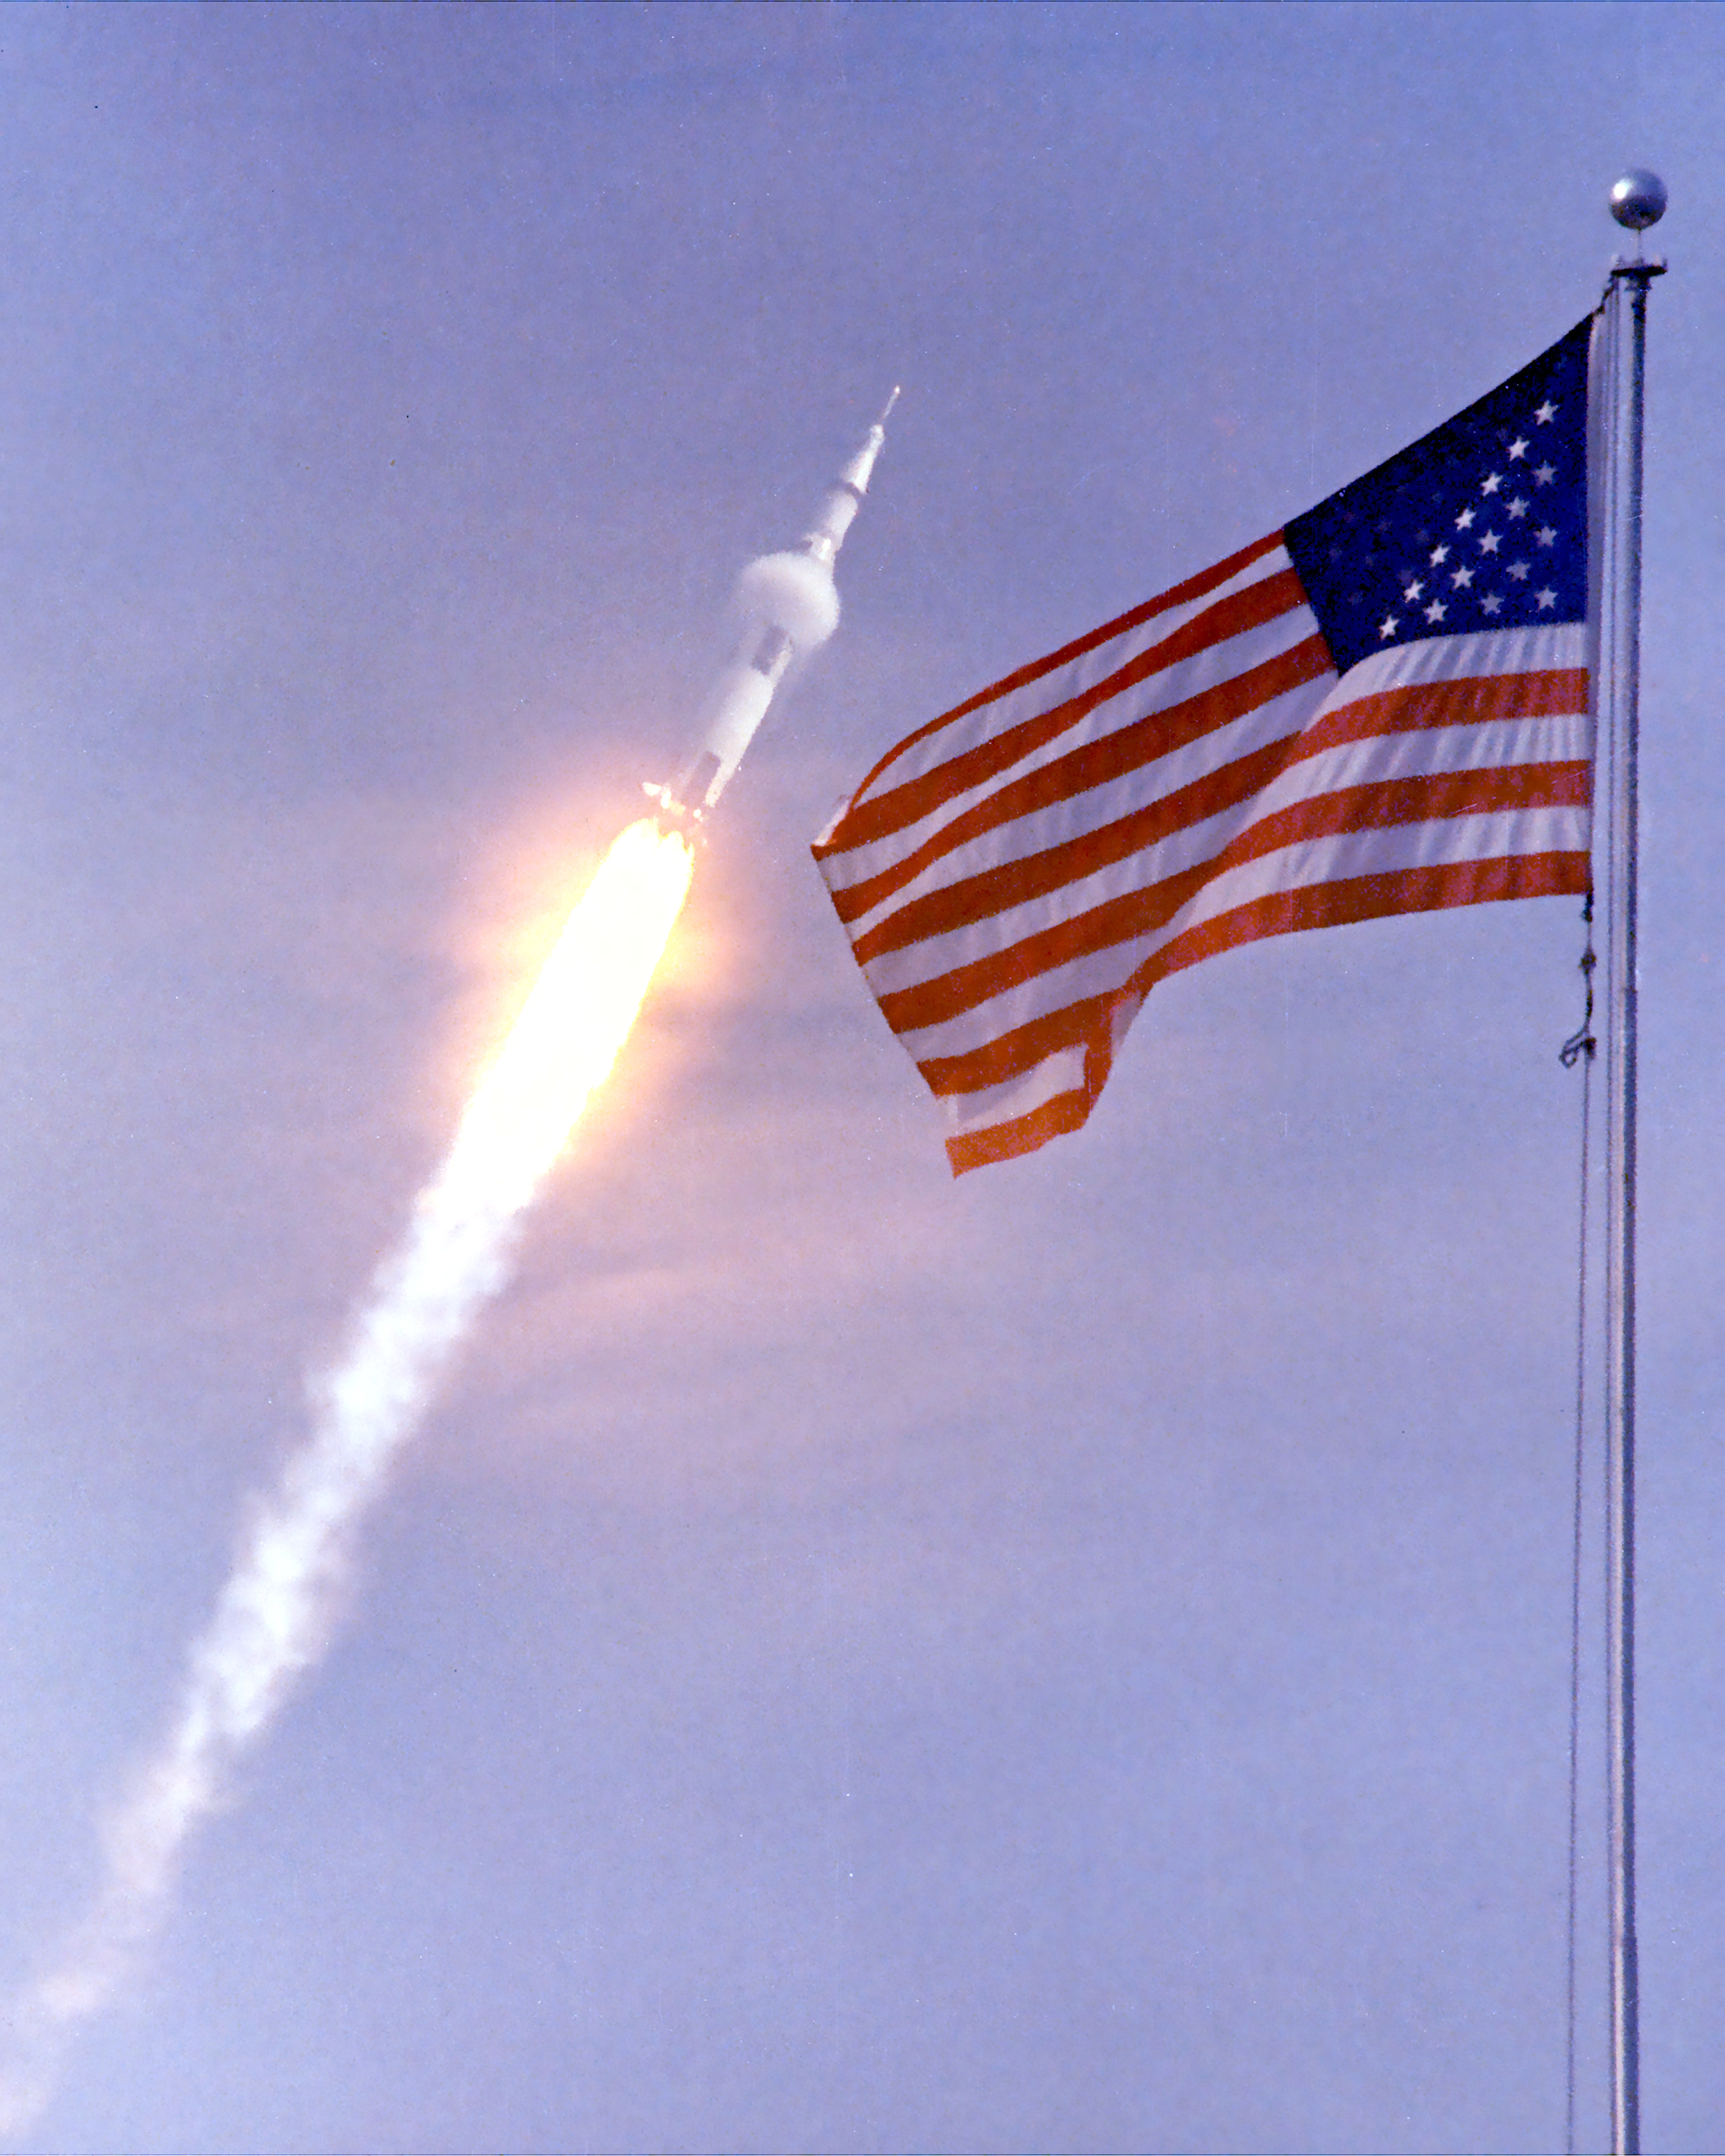
\includegraphics[width=0.92\textwidth]{images/saturn_v.jpg}
\captionof{figure}{Apollo 11 Saturn V launching on July 16, 1969. The rocket expels $13\,000\ \mathrm{kg\cdot s^{-1}}$ of hot combustion gas at $u_e \approx 2500\ \mathrm{m\cdot s^{-1}}$, generating $34\ \mathrm{MN}$ of thrust.}
\label{fig:saturn_v}
\end{minipage}\hfill
\begin{minipage}{0.48\textwidth}
\centering
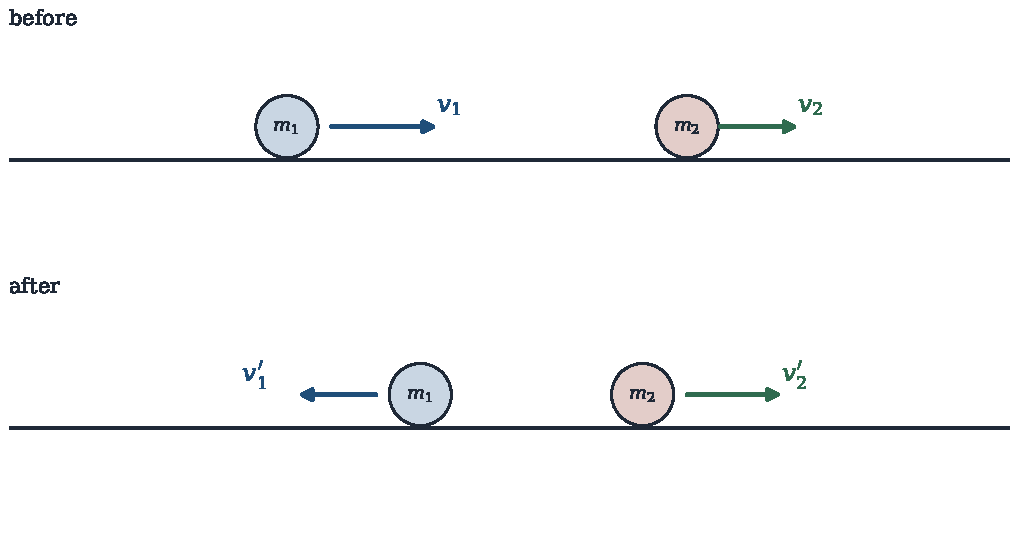
\includegraphics[width=0.92\textwidth]{figures/21_collision.pdf}
\captionof{figure}{Collision kinematics between two particles in the Laboratory frame (left) and the Center-of-Mass frame (right).}
\label{fig:collision}
\end{minipage}
\end{figure}

Consider a rocket of mass $m(t)$ moving at velocity $\vec{v}(t)$ at time $t$. During interval $\dd t$, the rocket ejects propellant mass $\dd m_e = -\dd m > 0$ backward with exit velocity $\vec{v}_e$ in the inertial frame.
The relative exhaust velocity with respect to the rocket is:
\begin{equation}
\vec{u}_e \eqdef \vec{v}_e - \vec{v}.
\end{equation}
The total momentum of the closed system (rocket + ejected parcel) at time $t$ is $\vec{P}(t) = m\vec{v}$.
At time $t + \dd t$, the rocket has mass $m + \dd m$ and velocity $\vec{v} + \dd\vec{v}$, while the ejected parcel has mass $-\dd m$ and velocity $\vec{v}_e = \vec{v} + \vec{u}_e$:
\[
\vec{P}(t + \dd t) = (m + \dd m)(\vec{v} + \dd\vec{v}) + (-\dd m)(\vec{v} + \vec{u}_e) = m\vec{v} + m\,\dd\vec{v} - \dd m\,\vec{u}_e + \mathcal{O}(\dd t^2).
\]
The net change in momentum is $\dd\vec{P} = m\,\dd\vec{v} - \dd m\,\vec{u}_e = \vec{F}_{\text{ext}}\,\dd t$.

\begin{lawbox}{Meshchersky's Rocket Dynamic Equation (1897)}
The instantaneous acceleration of a variable-mass vehicle is governed by:
\begin{equation}
m(t) \frac{\dd\vec{v}}{\dd t} = \vec{F}_{\text{ext}} + \frac{\dd m}{\dd t} \vec{u}_e = \vec{F}_{\text{ext}} + \vec{T}_{\text{thrust}},
\end{equation}
where the \textbf{rocket thrust} $\vec{T}_{\text{thrust}}$ is:
\begin{equation}
\vec{T}_{\text{thrust}} \eqdef \frac{\dd m}{\dd t} \vec{u}_e = \mu \norm{\vec{u}_e} \vec{u}_{\text{thrust}}, \qquad \mu = -\frac{\dd m}{\dd t} > 0.
\end{equation}
\end{lawbox}

\begin{historicalbox}{Konstantin Tsiolkovsky: Father of Astronautics}
\begin{minipage}{0.28\textwidth}
\centering
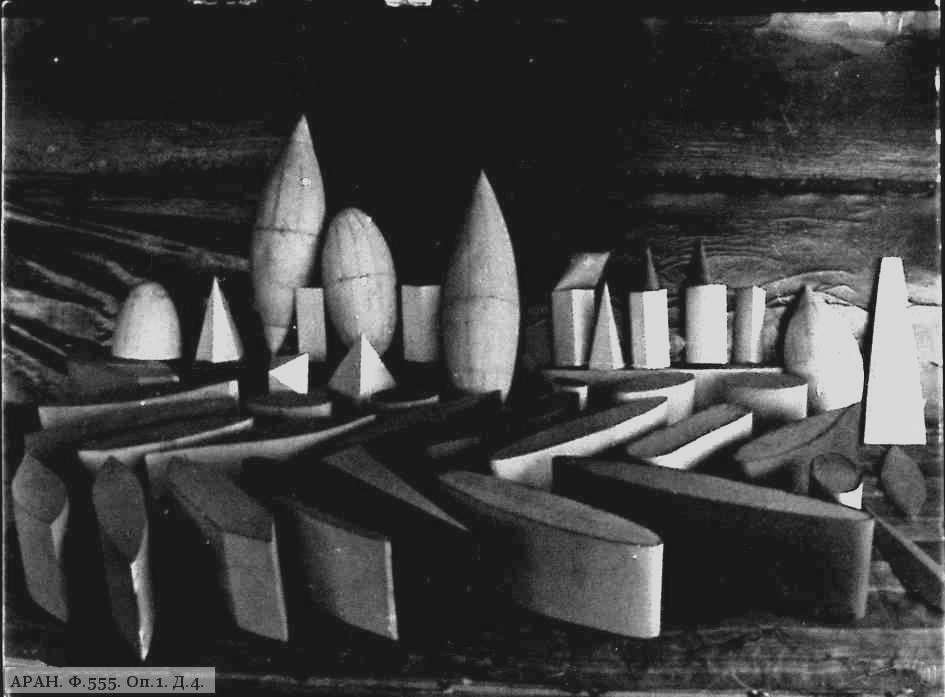
\includegraphics[width=0.92\textwidth]{images/tsiolkovsky.jpg}
\captionof{figure}{Konstantin Tsiolkovsky (1857--1935), Soviet pioneer of rocket science.}
\end{minipage}\hfill
\begin{minipage}{0.68\textwidth}
Working in near-total isolation as a deaf schoolteacher in the provincial Russian town of Kaluga, Konstantin Eduardovich Tsiolkovsky published his landmark paper in 1903: \emph{Exploration of Cosmic Space by Means of Reaction Devices}.

Tsiolkovsky mathematically proved that black gunpowder rockets could never escape Earth's gravity and proposed liquid-fuel engines running on liquid hydrogen and liquid oxygen. He invented multi-stage rocket trains, gyroscopic attitude stabilization, and closed-loop ecological life support, declaring: ``Earth is the cradle of humanity, but one cannot live in a cradle forever.''
\end{minipage}
\end{historicalbox}

\subsection{The Tsiolkovsky Rocket Equation}

In deep space where external forces vanish ($\vec{F}_{\text{ext}} = \vzero$), the 1D motion with propellant exhausted backward at speed $u_e$ satisfies:
\[
m\,\dd v = -u_e\,\dd m \implies \dd v = -u_e \frac{\dd m}{m}.
\]
Integrating from initial wet launch mass $m_0$ to final dry burnout mass $m_f$:
\[
\Delta v = \int_{m_0}^{m_f} -u_e \frac{\dd m}{m} = u_e \ln\left(\frac{m_0}{m_f}\right).
\]

\begin{lawbox}{The Tsiolkovsky Rocket Equation}
The characteristic burnout velocity increment $\Delta v$ achievable by a rocket in field-free space is:
\begin{equation}
\Delta v = u_e \ln\left(\frac{m_0}{m_f}\right) = g_0 I_{\text{sp}} \ln\left( \frac{m_0}{m_f} \right),
\end{equation}
where $I_{\text{sp}} \eqdef u_e/g_0$ is the engine \textbf{specific impulse} in seconds (with standard gravity $g_0 = 9.80665\ \mathrm{m\cdot s^{-2}}$).
In a uniform vertical gravitational field $\vec{g} = -g\,\khat$, vertical launch velocity is degraded by \textbf{gravity losses}:
\begin{equation}
v(t) = u_e \ln\left( \frac{m_0}{m(t)} \right) - g t.
\end{equation}
\end{lawbox}

\section{Collision Dynamics and Scattering Kinematics}

\begin{definitionbox}{Coefficient of Restitution (Newton, 1687)}
For a one-dimensional collision along the line of centers between particle 1 and particle 2, the \textbf{coefficient of restitution} $e$ is defined as the ratio of separation speed to approach speed:
\begin{equation}
e \eqdef \frac{|v_2' - v_1'|}{|v_1 - v_2|} = -\frac{v_2' - v_1'}{v_2 - v_1} \in [0, 1].
\end{equation}
\begin{itemize}[leftmargin=1.5em,itemsep=3pt]
  \item \textbf{Perfect Elastic Collision ($e = 1$):} Total kinetic energy is strictly conserved: $\Delta E_k = E_k' - E_k = 0$.
  \item \textbf{Partially Inelastic Collision ($0 < e < 1$):} Momentum is conserved, but kinetic energy is partially converted into internal deformation and heat: $\Delta E_k < 0$.
  \item \textbf{Perfect Inelastic (Plastic) Collision ($e = 0$):} The two bodies coalesce and move with a single common velocity $v_1' = v_2' = v_G$. The energy dissipation is maximized:
  \begin{equation}
  |\Delta E_k|_{\max} = \frac{1}{2} \mu (v_1 - v_2)^2, \qquad \mu \eqdef \frac{m_1 m_2}{m_1 + m_2}.
  \end{equation}
\end{itemize}
\end{definitionbox}

\section{Comprehensive Worked Examples}

\begin{workedexample}{Multi-Stage Rocket to Low Earth Orbit}
A spacecraft requires a total mission delta-v $\Delta v_{\text{req}} = 9200\ \mathrm{m\cdot s^{-1}}$ to reach Low Earth Orbit (including gravity and atmospheric drag losses). The rocket engines achieve an exhaust velocity $u_e = 3100\ \mathrm{m\cdot s^{-1}}$ ($I_{\text{sp}} \approx 316\ \mathrm{s}$).
\begin{enumerate}[leftmargin=1.4em,itemsep=3pt]
  \item Show that a single-stage rocket (SSTO) would require a structural-to-propellant mass ratio that is virtually impossible with modern aerospace alloys.
  \item Consider a two-stage rocket where each stage has identical exhaust velocity $u_e = 3100\ \mathrm{m\cdot s^{-1}}$ and provides half of the total velocity increment ($\Delta v_1 = \Delta v_2 = 4600\ \mathrm{m\cdot s^{-1}}$). Calculate the required mass ratio $m_{0i}/m_{fi}$ for each stage.
\end{enumerate}

\paragraph{Solution.}
\textbf{1. Single-Stage-to-Orbit (SSTO) Impossibility:}\\
Applying Tsiolkovsky's equation for a single stage:
\[
\Delta v = u_e \ln\left(\frac{m_0}{m_f}\right) \implies \frac{m_0}{m_f} = e^{\Delta v / u_e} = e^{9200 / 3100} = e^{2.9677} \approx 19.45.
\]
The final mass $m_f = m_{\text{structure}} + m_{\text{payload}}$ represents only:
\[
\frac{m_f}{m_0} = \frac{1}{19.45} \approx 0.0514 = 5.14\%.
\]
The propellant alone must constitute $94.86\%$ of the total launch mass. Because empty cryogenic tanks, rocket engines, turbopumps, avionics, and thermal insulation typically consume at least $6\text{--}8\%$ of dry structural mass, a single-stage chemical rocket cannot carry any useful payload to orbit.

\textbf{2. Two-Stage Rocket Staging Optimization:}\\
For each of the two stages:
\[
\Delta v_1 = \Delta v_2 = 4600\ \mathrm{m\cdot s^{-1}}.
\]
The required mass ratio for each stage is:
\[
\left(\frac{m_0}{m_f}\right)_1 = \left(\frac{m_0}{m_f}\right)_2 = e^{\Delta v_i / u_e} = e^{4600 / 3100} = e^{1.4839} \approx 4.41.
\]
The dry mass fraction for each individual stage is:
\[
\frac{m_{fi}}{m_{0i}} = \frac{1}{4.41} \approx 0.2268 = 22.7\%.
\]
Propellant constitutes only $77.3\%$ of each stage's mass! Dropping the empty first-stage tanks and heavy booster engines into the ocean eliminates the dead structural weight, allowing the second stage to ignite at high altitude and comfortably deliver several tons of scientific payload into orbit.
\end{workedexample}

\begin{workedexample}{Neutron Moderation and Energy Transfer in Nuclear Fission}
In a nuclear fission reactor, fission releases fast neutrons with kinetic energy $E_0 \approx 2.0\ \mathrm{MeV}$. To induce further fission in Uranium-235, these neutrons must be slowed down to thermal energies ($E_{\text{th}} \approx 0.025\ \mathrm{eV}$) through elastic collisions with stationary moderator nuclei of mass $M = A\,m_n$.
\begin{enumerate}[leftmargin=1.4em,itemsep=3pt]
  \item Derive the ratio of final to initial kinetic energy $E'/E_0$ for a head-on elastic collision.
  \item Compute the fractional energy loss $\xi \eqdef (E_0 - E')/E_0$ for:
  \begin{itemize}[leftmargin=1.2em]
    \item Ordinary Hydrogen ($A = 1$, light water $\mathrm{H_2O}$),
    \item Deuterium ($A = 2$, heavy water $\mathrm{D_2O}$),
    \item Carbon ($A = 12$, graphite),
    \item Uranium ($A = 238$).
  \end{itemize}
  \item Explain why light elements are uniquely suited as nuclear moderators.
\end{enumerate}

\paragraph{Solution.}
\textbf{1. Head-On Elastic Collision Kinematics:}\\
Let $m_n$ be the neutron mass and $M = A\,m_n$ be the target nucleus mass. In a head-on elastic collision with a stationary target ($v_2 = 0$):
\begin{align*}
m_n v_0 &= m_n v_1' + A m_n v_2', \\
\frac{1}{2}m_n v_0^2 &= \frac{1}{2}m_n (v_1')^2 + \frac{1}{2}A m_n (v_2')^2.
\end{align*}
Using Newton's restitution formula with $e = 1$:
\[
v_2' - v_1' = v_0 \implies v_2' = v_1' + v_0.
\]
Substituting $v_2'$ into the momentum equation:
\[
v_0 = v_1' + A(v_1' + v_0) = (A + 1)v_1' + A v_0 \implies v_1' = \left(\frac{1 - A}{1 + A}\right) v_0 = -\left(\frac{A - 1}{A + 1}\right) v_0.
\]
The final kinetic energy of the scattered neutron is:
\[
E' = \frac{1}{2}m_n (v_1')^2 = \left(\frac{A - 1}{A + 1}\right)^2 \left(\frac{1}{2}m_n v_0^2\right) \implies \frac{E'}{E_0} = \left(\frac{A - 1}{A + 1}\right)^2.
\]

\textbf{2. Fractional Energy Transferred:}\\
The fractional energy transferred to the target moderator nucleus is:
\[
\xi \eqdef \frac{E_0 - E'}{E_0} = 1 - \left(\frac{A - 1}{A + 1}\right)^2 = \frac{(A + 1)^2 - (A - 1)^2}{(A + 1)^2} = \frac{4A}{(A + 1)^2}.
\]
Evaluating $\xi$ for the different nuclei:
\begin{itemize}[leftmargin=1.5em,itemsep=3pt]
  \item \textbf{Hydrogen ($A = 1$):}
  \[
  \xi = \frac{4(1)}{(1 + 1)^2} = \frac{4}{4} = 1.000 \quad (\mathbf{100\%} \text{ energy transferred in a single collision!}).
  \]
  A fast neutron can lose its entire kinetic energy in a single billiard-ball collision with a proton of equal mass.
  \item \textbf{Deuterium ($A = 2$):}
  \[
  \xi = \frac{4(2)}{(2 + 1)^2} = \frac{8}{9} \approx 0.8889 = 88.9\%.
  \]
  \item \textbf{Carbon-12 ($A = 12$):}
  \[
  \xi = \frac{4(12)}{(12 + 1)^2} = \frac{48}{169} \approx 0.2840 = 28.4\%.
  \]
  \item \textbf{Uranium-238 ($A = 238$):}
  \[
  \xi = \frac{4(238)}{(238 + 1)^2} = \frac{952}{(239)^2} = \frac{952}{57\,121} \approx 0.0166 = 1.66\%.
  \]
\end{itemize}

\textbf{3. Physical Conclusion:}\\
Heavy elements like Uranium ($A = 238$) act as immovable brick walls: the light neutron bounces off elastically with virtually no energy loss ($98.3\%$ retained). Only light elements whose nuclear mass matches the neutron ($A \approx 1\text{--}2$) can absorb large fractions of kinetic energy per collision, allowing thermalization in just 18 to 25 collisions in water.
\end{workedexample}

\begin{workedexample}{Two-Dimensional Oblique Elastic Collision of Equal Masses}
A billiard ball $M_1$ of mass $m$ moving with speed $v_0$ along the $x$-axis collides elastically with an identical billiard ball $M_2$ of mass $m$ initially at rest. The collision is oblique (off-center).
\begin{enumerate}[leftmargin=1.4em,itemsep=3pt]
  \item Prove from vector conservation laws that the trajectories of the two balls after collision are \textbf{mutually perpendicular} ($90^\circ$ scattering angle), provided the collision is not head-on.
  \item If ball 1 is deflected by an angle $\theta_1 = 30^\circ$ relative to its initial incident direction, determine the deflection angle $\theta_2$ of ball 2, and the post-collision speeds $v_1'$ and $v_2'$.
\end{enumerate}

\paragraph{Solution.}
\textbf{1. Vector Proof of Orthogonality:}\\
Linear momentum conservation for two equal masses $m_1 = m_2 = m$ yields:
\[
m\vec{v}_0 = m\vec{v}_1' + m\vec{v}_2' \implies \vec{v}_0 = \vec{v}_1' + \vec{v}_2'.
\]
Because the collision is purely elastic, total kinetic energy is conserved:
\[
\frac{1}{2}m v_0^2 = \frac{1}{2}m (v_1')^2 + \frac{1}{2}m (v_2')^2 \implies v_0^2 = (v_1')^2 + (v_2')^2.
\]
Now take the scalar self-product (magnitude squared) of the momentum vector equation:
\[
v_0^2 = \vec{v}_0 \cdot \vec{v}_0 = (\vec{v}_1' + \vec{v}_2') \cdot (\vec{v}_1' + \vec{v}_2') = (v_1')^2 + (v_2')^2 + 2 (\vec{v}_1' \cdot \vec{v}_2').
\]
Comparing the two equations:
\[
(v_1')^2 + (v_2')^2 + 2 (\vec{v}_1' \cdot \vec{v}_2') = (v_1')^2 + (v_2')^2 \implies 2 (\vec{v}_1' \cdot \vec{v}_2') = 0.
\]
Therefore:
\begin{equation}
\vec{v}_1' \cdot \vec{v}_2' = 0.
\end{equation}
Unless one of the post-collision speeds vanishes (which occurs only for a direct head-on collision where $v_1' = 0$ and $v_2' = v_0$), the scalar product vanishes if and only if the velocity vectors are strictly orthogonal:
\[
\cos(\theta_1 + \theta_2) = 0 \implies \theta_1 + \theta_2 = 90^\circ.
\]

\textbf{2. Angles and Speeds for $\theta_1 = 30^\circ$:}\\
Since the total divergence angle is $90^\circ$:
\[
\theta_2 = 90^\circ - \theta_1 = 90^\circ - 30^\circ = 60^\circ.
\]
Projecting the momentum equation $\vec{v}_0 = \vec{v}_1' + \vec{v}_2'$ along the incident axis ($x$) and perpendicular axis ($y$):
\begin{align*}
v_1' \cos 30^\circ + v_2' \cos 60^\circ &= v_0, \\
v_1' \sin 30^\circ - v_2' \sin 60^\circ &= 0 \implies v_1'\left(\frac{1}{2}\right) = v_2'\left(\frac{\sqrt{3}}{2}\right) \implies v_1' = \sqrt{3}\,v_2'.
\end{align*}
Substituting $v_1'$ into the $x$-equation:
\[
(\sqrt{3} v_2')\left(\frac{\sqrt{3}}{2}\right) + v_2'\left(\frac{1}{2}\right) = v_0 \implies \frac{3}{2}v_2' + \frac{1}{2}v_2' = 2v_2' = v_0.
\]
Thus:
\[
v_2' = \frac{1}{2} v_0 = 0.50\,v_0, \qquad v_1' = \frac{\sqrt{3}}{2} v_0 \approx 0.866\,v_0.
\]
Checking kinetic energy conservation:
\[
(v_1')^2 + (v_2')^2 = \left(\frac{\sqrt{3}}{2} v_0\right)^2 + \left(\frac{1}{2} v_0\right)^2 = \left(\frac{3}{4} + \frac{1}{4}\right)v_0^2 = v_0^2.
\]
Energy and momentum are verified in every detail.
\end{workedexample}


\appendix
\part*{Appendices}
\addcontentsline{toc}{part}{Appendices}

\chapter{Mathematical Toolbox for Classical Mechanics}
\label{app:math}

This mathematical appendix compiles the fundamental vector calculus, curvilinear coordinate formulas, vector identities, and asymptotic series expansions used throughout classical point mechanics.

\section{Curvilinear Coordinate Systems}

\subsection{1. Cartesian Coordinates $(x, y, z)$}
\begin{itemize}[leftmargin=1.5em,itemsep=3pt]
  \item \textbf{Position Vector:}
  \[
  \vec{r} = x\,\ihat + y\,\jhat + z\,\khat.
  \]
  \item \textbf{Velocity Vector:}
  \[
  \vec{v} = \dot{x}\,\ihat + \dot{y}\,\jhat + \dot{z}\,\khat.
  \]
  \item \textbf{Acceleration Vector:}
  \[
  \vec{a} = \ddot{x}\,\ihat + \ddot{y}\,\jhat + \ddot{z}\,\khat.
  \]
  \item \textbf{Infinitesimal Displacement and Volume Element:}
  \[
  \dd\vec{r} = \dd x\,\ihat + \dd y\,\jhat + \dd z\,\khat, \qquad \dd V = \dd x\,\dd y\,\dd z.
  \]
  \item \textbf{Differential Vector Operators:}
  \begin{align*}
  \vec{\nabla} \Phi &= \frac{\partial\Phi}{\partial x}\,\ihat + \frac{\partial\Phi}{\partial y}\,\jhat + \frac{\partial\Phi}{\partial z}\,\khat, \\
  \vec{\nabla} \cdot \vec{A} &= \frac{\partial A_x}{\partial x} + \frac{\partial A_y}{\partial y} + \frac{\partial A_z}{\partial z}, \\
  \vec{\nabla} \times \vec{A} &= \left(\frac{\partial A_z}{\partial y} - \frac{\partial A_y}{\partial z}\right)\ihat + \left(\frac{\partial A_x}{\partial z} - \frac{\partial A_z}{\partial x}\right)\jhat + \left(\frac{\partial A_y}{\partial x} - \frac{\partial A_x}{\partial y}\right)\khat, \\
  \nabla^2 \Phi &= \frac{\partial^2\Phi}{\partial x^2} + \frac{\partial^2\Phi}{\partial y^2} + \frac{\partial^2\Phi}{\partial z^2}.
  \end{align*}
\end{itemize}

\subsection{2. Cylindrical Coordinates $(r, \theta, z)$}
\begin{itemize}[leftmargin=1.5em,itemsep=3pt]
  \item \textbf{Coordinate Transformation:}
  \[
  x = r\cos\theta, \qquad y = r\sin\theta, \qquad z = z.
  \]
  \item \textbf{Basis Vectors:}
  \[
  \ur = \cos\theta\,\ihat + \sin\theta\,\jhat, \qquad \ut = -\sin\theta\,\ihat + \cos\theta\,\jhat, \qquad \khat = \khat.
  \]
  \item \textbf{Kinematic Vectors:}
  \begin{align*}
  \vec{r} &= r\,\ur + z\,\khat, \\
  \vec{v} &= \dot{r}\,\ur + r\dot{\theta}\,\ut + \dot{z}\,\khat, \\
  \vec{a} &= (\ddot{r} - r\dot{\theta}^2)\,\ur + (r\ddot{\theta} + 2\dot{r}\dot{\theta})\,\ut + \ddot{z}\,\khat.
  \end{align*}
  \item \textbf{Displacement and Volume Elements:}
  \[
  \dd\vec{r} = \dd r\,\ur + r\,\dd\theta\,\ut + \dd z\,\khat, \qquad \dd V = r\,\dd r\,\dd\theta\,\dd z.
  \]
  \item \textbf{Vector Differential Operators:}
  \begin{align*}
  \vec{\nabla} \Phi &= \frac{\partial\Phi}{\partial r}\,\ur + \frac{1}{r}\frac{\partial\Phi}{\partial\theta}\,\ut + \frac{\partial\Phi}{\partial z}\,\khat, \\
  \vec{\nabla} \cdot \vec{A} &= \frac{1}{r}\frac{\partial(r A_r)}{\partial r} + \frac{1}{r}\frac{\partial A_\theta}{\partial\theta} + \frac{\partial A_z}{\partial z}, \\
  \vec{\nabla} \times \vec{A} &= \left(\frac{1}{r}\frac{\partial A_z}{\partial\theta} - \frac{\partial A_\theta}{\partial z}\right)\ur + \left(\frac{\partial A_r}{\partial z} - \frac{\partial A_z}{\partial r}\right)\ut + \frac{1}{r}\left(\frac{\partial(r A_\theta)}{\partial r} - \frac{\partial A_r}{\partial\theta}\right)\khat.
  \end{align*}
\end{itemize}

\subsection{3. Spherical Coordinates $(r, \theta, \phi)$}
\begin{itemize}[leftmargin=1.5em,itemsep=3pt]
  \item \textbf{Coordinate Transformation:} ($r \ge 0$, $\theta \in [0, \pi]$ colatitude, $\phi \in [0, 2\pi)$ azimuth)
  \[
  x = r\sin\theta\cos\phi, \qquad y = r\sin\theta\sin\phi, \qquad z = r\cos\theta.
  \]
  \item \textbf{Kinematic Vectors:}
  \begin{align*}
  \vec{r} &= r\,\ur, \\
  \vec{v} &= \dot{r}\,\ur + r\dot{\theta}\,\ut + r\dot{\phi}\sin\theta\,\uphi, \\
  a_r &= \ddot{r} - r\dot{\theta}^2 - r\dot{\phi}^2\sin^2\theta, \\
  a_\theta &= r\ddot{\theta} + 2\dot{r}\dot{\theta} - r\dot{\phi}^2\sin\theta\cos\theta, \\
  a_\phi &= r\ddot{\phi}\sin\theta + 2\dot{r}\dot{\phi}\sin\theta + 2r\dot{\theta}\dot{\phi}\cos\theta = \frac{1}{r\sin\theta}\frac{\dd}{\dd t}(r^2\dot{\phi}\sin^2\theta).
  \end{align*}
  \item \textbf{Volume and Area Elements:}
  \[
  \dd V = r^2\sin\theta\,\dd r\,\dd\theta\,\dd\phi, \qquad \dd\Omega = \sin\theta\,\dd\theta\,\dd\phi.
  \]
  \item \textbf{Gradient in Spherical Coordinates:}
  \[
  \vec{\nabla}\Phi = \frac{\partial\Phi}{\partial r}\,\ur + \frac{1}{r}\frac{\partial\Phi}{\partial\theta}\,\ut + \frac{1}{r\sin\theta}\frac{\partial\Phi}{\partial\phi}\,\uphi.
  \]
\end{itemize}

\subsection{4. Frenet-Serret Intrinsic Coordinates $(\utt, \un, \ub)$}
For a 3D curve parametrized by arc length $s$:
\begin{equation}
\frac{\dd\utt}{\dd s} = \frac{1}{R_c}\,\un, \qquad \frac{\dd\un}{\dd s} = -\frac{1}{R_c}\,\utt + \tau\,\ub, \qquad \frac{\dd\ub}{\dd s} = -\tau\,\un,
\end{equation}
where $R_c$ is the local radius of curvature and $\tau$ is the torsion.
Kinematic decomposition:
\begin{equation}
\vec{v} = v\,\utt, \qquad \vec{a} = \dot{v}\,\utt + \frac{v^2}{R_c}\,\un.
\end{equation}

\section{Essential Vector Algebra and Calculus Identities}

Let $\vec{A}, \vec{B}, \vec{C}, \vec{D}$ be vector fields and $\Phi, \Psi$ be scalar fields:
\begin{align}
\vec{A} \times (\vec{B} \times \vec{C}) &= (\vec{A} \cdot \vec{C})\vec{B} - (\vec{A} \cdot \vec{B})\vec{C} \quad \text{(BAC-CAB Rule)}, \\
\vec{A} \cdot (\vec{B} \times \vec{C}) &= \vec{B} \cdot (\vec{C} \times \vec{A}) = \vec{C} \cdot (\vec{A} \times \vec{B}) \quad \text{(Scalar Triple Product)}, \\
(\vec{A} \times \vec{B}) \cdot (\vec{C} \times \vec{D}) &= (\vec{A} \cdot \vec{C})(\vec{B} \cdot \vec{D}) - (\vec{A} \cdot \vec{D})(\vec{B} \cdot \vec{C}) \quad \text{(Binet-Cauchy Identity)}, \\
\vec{\nabla}(\Phi\Psi) &= \Phi\,\vec{\nabla}\Psi + \Psi\,\vec{\nabla}\Phi, \\
\vec{\nabla} \cdot (\Phi\vec{A}) &= \Phi(\vec{\nabla}\cdot\vec{A}) + \vec{A}\cdot\vec{\nabla}\Phi, \\
\vec{\nabla} \times (\Phi\vec{A}) &= \Phi(\vec{\nabla}\times\vec{A}) + (\vec{\nabla}\Phi)\times\vec{A}, \\
\vec{\nabla} \times (\vec{\nabla}\Phi) &\equiv \vzero \quad \text{(The curl of a gradient is identically zero)}, \\
\vec{\nabla} \cdot (\vec{\nabla}\times\vec{A}) &\equiv 0 \quad \text{(The divergence of a curl is identically zero)}, \\
\vec{\nabla} \times (\vec{\nabla}\times\vec{A}) &= \vec{\nabla}(\vec{\nabla}\cdot\vec{A}) - \nabla^2\vec{A}.
\end{align}

\section{Standard Taylor Series Expansions ($x \to 0$)}

\begin{align}
(1 + x)^\alpha &= 1 + \alpha x + \frac{\alpha(\alpha-1)}{2!} x^2 + \frac{\alpha(\alpha-1)(\alpha-2)}{3!} x^3 + \mathcal{O}(x^4), \\
\frac{1}{1 - x} &= 1 + x + x^2 + x^3 + \mathcal{O}(x^4), \\
\sin x &= x - \frac{x^3}{6} + \frac{x^5}{120} + \mathcal{O}(x^7), \\
\cos x &= 1 - \frac{x^2}{2} + \frac{x^4}{24} - \frac{x^6}{720} + \mathcal{O}(x^8), \\
\tan x &= x + \frac{x^3}{3} + \frac{2x^5}{15} + \mathcal{O}(x^7), \\
e^x &= 1 + x + \frac{x^2}{2} + \frac{x^3}{6} + \frac{x^4}{24} + \mathcal{O}(x^5), \\
\ln(1 + x) &= x - \frac{x^2}{2} + \frac{x^3}{3} - \frac{x^4}{4} + \mathcal{O}(x^5), \\
\sinh x &= x + \frac{x^3}{6} + \frac{x^5}{120} + \mathcal{O}(x^7), \\
\cosh x &= 1 + \frac{x^2}{2} + \frac{x^4}{24} + \mathcal{O}(x^6).
\end{align}

\chapter{Physical Constants and Astronomical Data}
\label{app:constants}

This appendix provides authoritative values for fundamental physical constants (CODATA recommended values) and standard astronomical parameters of the Solar System.

\section{Fundamental Physical Constants}

\begin{center}
\renewcommand{\arraystretch}{1.3}
\begin{longtable}{@{}llll@{}}
\toprule
\textbf{Physical Quantity} & \textbf{Symbol} & \textbf{Value} & \textbf{SI Unit} \\
\midrule
\endhead
Speed of light in vacuum & $c$ & $2.997\,924\,58 \times 10^8$ & $\mathrm{m\cdot s^{-1}}$ (exact) \\
Newtonian gravitational constant & $G$ & $6.674\,30(15) \times 10^{-11}$ & $\mathrm{m^3\cdot kg^{-1}\cdot s^{-2}}$ \\
Standard acceleration of gravity & $g_0$ & $9.806\,65$ & $\mathrm{m\cdot s^{-2}}$ (exact) \\
Planck constant & $h$ & $6.626\,070\,15 \times 10^{-34}$ & $\mathrm{J\cdot s}$ (exact) \\
Reduced Planck constant & $\hbar = h/(2\pi)$ & $1.054\,571\,817 \times 10^{-34}$ & $\mathrm{J\cdot s}$ \\
Elementary charge & $e$ & $1.602\,176\,634 \times 10^{-19}$ & $\mathrm{C}$ (exact) \\
Vacuum permittivity & $\varepsilon_0 = 1/(\mu_0 c^2)$ & $8.854\,187\,8128 \times 10^{-12}$ & $\mathrm{F\cdot m^{-1}}$ \\
Coulomb constant & $k_e = \frac{1}{4\pi\varepsilon_0}$ & $8.987\,551\,7923 \times 10^9$ & $\mathrm{N\cdot m^2\cdot C^{-2}}$ \\
Electron rest mass & $m_e$ & $9.109\,383\,7015 \times 10^{-31}$ & $\mathrm{kg}$ \\
Proton rest mass & $m_p$ & $1.672\,621\,923\,69 \times 10^{-27}$ & $\mathrm{kg}$ \\
Neutron rest mass & $m_n$ & $1.674\,927\,498\,04 \times 10^{-27}$ & $\mathrm{kg}$ \\
Atomic mass unit & $1\ \mathrm{u} = \frac{1}{12}m(^{12}\mathrm{C})$ & $1.660\,539\,066\,60 \times 10^{-27}$ & $\mathrm{kg}$ \\
Avogadro constant & $N_A$ & $6.022\,140\,76 \times 10^{23}$ & $\mathrm{mol^{-1}}$ (exact) \\
Boltzmann constant & $k_B$ & $1.380\,649 \times 10^{-23}$ & $\mathrm{J\cdot K^{-1}}$ (exact) \\
Molar gas constant & $R = N_A k_B$ & $8.314\,462\,618$ & $\mathrm{J\cdot mol^{-1}\cdot K^{-1}}$ \\
\bottomrule
\end{longtable}
\end{center}

\section{Terrestrial and Lunar Parameters}

\begin{center}
\renewcommand{\arraystretch}{1.3}
\begin{tabular}{@{}llll@{}}
\toprule
\textbf{Parameter} & \textbf{Symbol} & \textbf{Value} & \textbf{Unit} \\
\midrule
Earth total mass & $M_\oplus$ & $5.9722 \times 10^{24}$ & $\mathrm{kg}$ \\
Earth mean radius & $R_\oplus$ & $6.3710 \times 10^6$ & $\mathrm{m}$ \\
Earth equatorial radius & $R_{\text{eq}}$ & $6.3781 \times 10^6$ & $\mathrm{m}$ \\
Earth polar radius & $R_{\text{pol}}$ & $6.3568 \times 10^6$ & $\mathrm{m}$ \\
Earth geometric flattening & $f = (R_{\text{eq}} - R_{\text{pol}})/R_{\text{eq}}$ & $1/298.257$ & --- \\
Earth standard gravitational parameter & $\mu_\oplus = G M_\oplus$ & $3.986\,004\,418 \times 10^{14}$ & $\mathrm{m^3\cdot s^{-2}}$ \\
Sidereal rotation day & $T_{\text{sid}}$ & $86\,164.09$ & $\mathrm{s}$ ($23^\mathrm{h}\,56^\mathrm{m}\,04^\mathrm{s}$) \\
Earth diurnal angular velocity & $\Omega_\oplus = 2\pi/T_{\text{sid}}$ & $7.292\,115 \times 10^{-5}$ & $\mathrm{rad\cdot s^{-1}}$ \\
Mean Earth-Sun distance (Astronomical Unit) & $1\ \mathrm{AU}$ & $1.495\,978\,707 \times 10^{11}$ & $\mathrm{m}$ (exact) \\
Sidereal year & $1\ \mathrm{yr}$ & $3.155\,815 \times 10^7$ & $\mathrm{s}$ ($365.256\ \mathrm{d}$) \\
\midrule
Moon mass & $M_{\text{Moon}}$ & $7.342 \times 10^{22}$ & $\mathrm{kg}$ ($0.0123\,M_\oplus$) \\
Moon mean radius & $R_{\text{Moon}}$ & $1.7374 \times 10^6$ & $\mathrm{m}$ \\
Moon surface gravity & $g_{\text{Moon}}$ & $1.62$ & $\mathrm{m\cdot s^{-2}}$ ($0.165\,g_0$) \\
Mean Earth-Moon center distance & $d_{\oplus\text{-Moon}}$ & $3.844 \times 10^8$ & $\mathrm{m}$ \\
\bottomrule
\end{tabular}
\end{center}

\section{Solar and Planetary Orbital Data}

\begin{center}
\renewcommand{\arraystretch}{1.25}
\begin{longtable}{@{}llllll@{}}
\toprule
\textbf{Body} & \textbf{Mass ($\mathrm{kg}$)} & \textbf{Mean Radius ($\mathrm{km}$)} & \textbf{Semi-Major Axis ($a$)} & \textbf{Period ($T$)} & \textbf{Eccentricity ($e$)} \\
\midrule
\endhead
\textbf{Sun} & $1.9885 \times 10^{30}$ & $696\,340$ & --- & --- & --- \\
\textbf{Mercury} & $3.3011 \times 10^{23}$ & $2\,439.7$ & $0.3871\ \mathrm{AU}$ & $87.97\ \mathrm{d}$ & $0.2056$ \\
\textbf{Venus} & $4.8675 \times 10^{24}$ & $6\,051.8$ & $0.7233\ \mathrm{AU}$ & $224.70\ \mathrm{d}$ & $0.0067$ \\
\textbf{Earth} & $5.9722 \times 10^{24}$ & $6\,371.0$ & $1.0000\ \mathrm{AU}$ & $365.26\ \mathrm{d}$ & $0.0167$ \\
\textbf{Mars} & $6.4171 \times 10^{23}$ & $3\,389.5$ & $1.5237\ \mathrm{AU}$ & $686.98\ \mathrm{d}$ & $0.0934$ \\
\textbf{Jupiter} & $1.8982 \times 10^{27}$ & $69\,911$ & $5.2044\ \mathrm{AU}$ & $11.86\ \mathrm{yr}$ & $0.0489$ \\
\textbf{Saturn} & $5.6834 \times 10^{26}$ & $58\,232$ & $9.5826\ \mathrm{AU}$ & $29.46\ \mathrm{yr}$ & $0.0565$ \\
\textbf{Uranus} & $8.6810 \times 10^{25}$ & $25\,362$ & $19.218\ \mathrm{AU}$ & $84.01\ \mathrm{yr}$ & $0.0472$ \\
\textbf{Neptune} & $1.0241 \times 10^{26}$ & $24\,622$ & $30.070\ \mathrm{AU}$ & $164.79\ \mathrm{yr}$ & $0.0086$ \\
\bottomrule
\end{longtable}
\end{center}


\end{document}
